\documentclass[a4paper,11pt,twoside]{book}
\usepackage[T1]{fontenc}
\usepackage[utf8]{inputenc}
\usepackage[french]{babel}
\usepackage[left=3cm,right=3cm,headheight=15pt,twoside]{geometry}

% custom headers/footers
\usepackage{fancyhdr}
\pagestyle{fancy}
\fancyhead[ro,re,c]{}
\fancyhead[le]{\begin{minipage}[b]{\textwidth}\raggedleft\small\bfseries\slshape\nouppercase\leftmark\\\end{minipage}}
\fancyhead[lo]{\begin{minipage}[b]{\textwidth}\raggedright\small\bfseries\slshape\nouppercase\rightmark\\\end{minipage}}
\fancyfoot[r,c]{}
\fancyfoot[le]{\raggedright\small\thepage}
\fancyfoot[lo]{\raggedleft\small\thepage}

%interligne
%\linespread{1.4}
% a loader *avant* hyperref: http://tex.stackexchange.com/a/79551/32098
\usepackage{titletoc}
\usepackage[toctitles]{titlesec}

% liens internes
\usepackage[hidelinks,pagebackref=true]{hyperref}
% liens externes
\usepackage{url}


% couleurs
\usepackage{xcolor}

% frames
\usepackage{framed}

% sauts de ligne entre les paragraphes, plutot qu'une simple indentation
\usepackage{parskip}

% evite les erreurs de justification
% http://tex.stackexchange.com/questions/174903/justified-text-extending-beyond-margin
\usepackage{microtype}

% listing configuration pour le code
\usepackage{courier,listings}

\definecolor{superlightgray}{gray}{0.95}
\definecolor{lightgray}{gray}{0.75}
\definecolor{darkgray}{gray}{0.25}
\definecolor{superdarkgray}{gray}{0.25}

% Define minizinc language
\lstdefinelanguage{minizinc} { %
    morekeywords={set,of,min,max,in,int,var,show,show_int,constraint,include,forall,array},
    sensitive=true,
    morecomment=[l]{\%},
    morestring=[b]" % defines that strings are enclosed in double quotes
}
% general parameters
\lstset{ %
  backgroundcolor=\color{superlightgray},   % choose the background color; you must add \usepackage{color} or \usepackage{xcolor}
  basicstyle=\tiny\ttfamily,                % the size of the fonts that are used for the code
  breakatwhitespace=false,                  % sets if automatic breaks should only happen at whitespace
  breaklines=false,                         % sets automatic line breaking
  captionpos=b,                             % sets the caption-position to bottom
  commentstyle=\itshape\color{gray},        % comment style
  deletekeywords={...},                     % if you want to delete keywords from the given language
  escapeinside={\%*}{*)},                   % if you want to add LaTeX within your code
  extendedchars=true,                       % lets you use non-ASCII characters; for 8-bits encodings only, does not work with UTF-8
  frame=single,	                            % adds a frame around the code
  keepspaces=true,                          % keeps spaces in text, useful for keeping indentation of code (possibly needs columns=flexible)
  keywordstyle=\bfseries,                   % keyword style
  language=minizinc,                        % the language of the code
  % otherkeywords={},                       % if you want to add more keywords to the set
  numbers=left,                             % where to put the line-numbers; possible values are (none, left, right)
  numbersep=5pt,                            % how far the line-numbers are from the code
  numberstyle=\tiny\color{lightgray},       % the style that is used for the line-numbers
  rulecolor=\color{black},                  % if not set, the frame-color may be changed on line-breaks within not-black text (e.g. comments (green here))
  showspaces=false,                         % show spaces everywhere adding particular underscores; it overrides 'showstringspaces'
  showstringspaces=false,                   % underline spaces within strings only
  showtabs=false,                           % show tabs within strings adding particular underscores
  stepnumber=2,                             % the step between two line-numbers. If it's 1, each line will be numbered
  stringstyle=\color{darkgray},             % string literal style
  tabsize=2,	                            % sets default tabsize to 2 spaces
  % title=\lstname                          % show the filename of files included with \lstinputlisting; also try caption instead of title
}

% packages et commandes pour les figures
\usepackage{adjustbox}
\usepackage{arydshln,tabulary,multirow,booktabs,array,bigdelim}
\usepackage{graphicx}
\usepackage{pbox}
\usepackage{rotating}
\usepackage{tikz}
\usetikzlibrary{calc,mindmap,trees,fit,positioning}
\tikzset{concept/.append style={fill={none}}}

\newlength{\mytablewidth}
\newlength{\myfirstcolwidth}
\newlength{\mycolwidth}
\newlength{\mylastcolwidth}
\newcommand\mrows[1]{\multirow{#1}{\mycolwidth}{}}
% accolade verticale sur plusieurs lignes
% http://tex.stackexchange.com/a/218053/32098
\newcommand\multibrace[3]{\rdelim\}{#1}{3mm}[\pbox{#2}{#3}]}
% pour laisser une "marque" utilisable plus tard avec tikz
% utile pour tracer des fleches au dessus des tableaux par exemple
\newcommand\tikzmark[1]{\tikz[overlay,remember picture] \coordinate (#1);}
\newcommand\centbf[1]{\centering\textbf{#1}}
\newcommand\centit[1]{\centering\textit{#1}}

% checkmarks
% http://tex.stackexchange.com/a/132800/32098
\def\checkmark{\tikz\fill[scale=0.4](0,.35) -- (.25,0) -- (1,.7) -- (.25,.15) -- cycle;}
\def\scalecheck{\resizebox{\widthof{\checkmark}*\ratio{\widthof{x}}{\widthof{\normalsize x}}}{!}{\checkmark}}

% http://tex.stackexchange.com/questions/245825/how-to-draw-an-ekg-tracing-with-tikz/245839#245839
% http://tex.stackexchange.com/questions/173569/tikz-pic-parameter
% carte de france
% TODO: rendre les couleurs parametrables
\definecolor{cFFFFFF}{RGB}{255,255,255}
\definecolor{cE3ECF6}{RGB}{227,236,246}
\definecolor{cBCBD43}{RGB}{188,189,67}
\definecolor{c999999}{RGB}{153,153,153}
\definecolor{c666666}{RGB}{102,102,102} % frontieres et regions
\definecolor{cCCCCCC}{RGB}{204,204,204}
\tikzset{
    pics/france/.style args={scale #1}{
        code={
            \begin{scope}[y=0.80pt, x=0.80pt, yscale=-1.000000, xscale=1.000000, inner sep=0pt, outer sep=0pt, scale=#1]
                %\definecolor{cFFFFFF}{RGB}{255,255,255}
%\definecolor{cE3ECF6}{RGB}{227,236,246}
%\definecolor{cBCBD43}{RGB}{188,189,67}
%\definecolor{c999999}{RGB}{153,153,153}
%\definecolor{c666666}{RGB}{102,102,102} % frontieres et regions
%\definecolor{cCCCCCC}{RGB}{204,204,204}


%\begin{tikzpicture}[y=0.80pt, x=0.80pt, yscale=-1.000000, xscale=1.000000, inner sep=0pt, outer sep=0pt, scale=1]
\begin{scope}% departements
  \begin{scope}% g4612
    \begin{scope}% g4614
      \begin{scope}% g4616
        % path4618
        \path[draw,color=cFFFFFF,densely dotted] (442.2000,80.2000) -- (439.0000,73.7000) --
          (439.0000,69.1000) -- (441.9000,63.4000) -- (438.9000,61.6000) --
          (434.3000,66.5000) -- (432.4000,73.7000) -- (422.6000,78.1000) --
          (416.5000,76.1000) -- (413.3000,76.9000) -- (414.3000,83.3000) --
          (412.7000,87.2000) -- (414.3000,90.6000) -- (408.6000,98.7000) --
          (405.5000,99.1000) -- (405.9000,115.1000) -- (413.4000,116.2000) --
          (424.5000,123.6000) -- (447.0000,125.7000) -- (447.0000,125.6000) --
          (451.7000,121.5000) -- (450.2000,118.7000) -- (453.8000,113.0000) --
          (452.8000,103.2000) -- (455.0000,100.9000) -- (461.4000,103.2000) --
          (463.7000,100.2000) -- (465.7000,98.9000) -- (462.1000,99.2000) --
          (462.1000,95.6000) -- (455.3000,93.9000) -- (447.8000,87.3000) --
          (441.1000,87.5000) -- (442.2000,80.2000) -- cycle;

        % path4620
        \path[draw,color=cFFFFFF,densely dotted] (455.0000,100.9000) -- (452.8000,103.2000) --
          (453.8000,113.0000) -- (450.2000,118.7000) -- (451.7000,121.5000) --
          (447.0000,125.6000) -- (447.0000,125.7000) -- (449.5000,135.9000) --
          (448.4000,140.4000) -- (451.3000,141.9000) -- (450.6000,146.4000) --
          (447.2000,147.5000) -- (445.9000,154.1000) -- (449.5000,159.2000) --
          (450.0000,163.8000) -- (453.8000,169.6000) -- (472.8000,181.2000) --
          (480.6000,177.4000) -- (484.0000,178.0000) -- (486.2000,175.4000) --
          (486.4000,172.3000) -- (483.6000,170.0000) -- (485.4000,166.8000) --
          (484.0000,157.1000) -- (486.5000,141.7000) -- (487.5000,138.6000) --
          (482.0000,125.7000) -- (483.7000,119.1000) -- (482.3000,116.1000) --
          (477.4000,110.6000) -- (471.3000,112.9000) -- (469.9000,106.9000) --
          (469.6000,107.0000) -- (465.7000,98.9000) -- (463.7000,100.2000) --
          (461.4000,103.2000) -- (455.0000,100.9000) -- cycle;

        % path4622
        \path[draw,color=cFFFFFF,densely dotted] (469.9000,106.9000) -- (471.3000,112.9000) --
          (477.4000,110.6000) -- (482.3000,116.1000) -- (483.7000,119.1000) --
          (482.0000,125.7000) -- (487.5000,138.6000) -- (486.5000,141.7000) --
          (484.0000,157.1000) -- (485.4000,166.8000) -- (483.6000,170.0000) --
          (486.4000,172.3000) -- (486.2000,175.4000) -- (492.6000,176.1000) --
          (492.5000,179.4000) -- (497.1000,184.8000) -- (503.6000,184.0000) --
          (504.8000,180.9000) -- (510.8000,178.7000) -- (513.5000,180.6000) --
          (520.3000,179.5000) -- (526.2000,175.3000) -- (528.0000,178.2000) --
          (534.8000,180.1000) -- (546.7000,171.5000) -- (548.4000,171.0000) --
          (546.3000,169.6000) -- (544.0000,166.6000) -- (527.9000,160.5000) --
          (521.9000,156.3000) -- (512.4000,154.6000) -- (509.3000,148.8000) --
          (509.8000,145.6000) -- (496.9000,141.1000) -- (491.9000,132.7000) --
          (495.2000,132.5000) -- (494.1000,126.2000) -- (495.8000,122.8000) --
          (494.5000,118.8000) -- (491.7000,117.0000) -- (489.0000,106.4000) --
          (485.0000,103.0000) -- (477.3000,103.0000) -- (475.9000,106.1000) --
          (469.9000,106.9000) -- cycle;

        % path4624
        \path[draw,color=cFFFFFF,densely dotted] (489.0000,106.4000) -- (491.7000,117.0000) --
          (494.5000,118.8000) -- (495.8000,122.8000) -- (494.1000,126.2000) --
          (495.2000,132.5000) -- (491.9000,132.7000) -- (496.9000,141.1000) --
          (509.8000,145.6000) -- (509.3000,148.8000) -- (512.4000,154.6000) --
          (521.9000,156.3000) -- (527.9000,160.5000) -- (544.0000,166.6000) --
          (546.3000,169.6000) -- (550.2000,169.9000) -- (552.7000,168.0000) --
          (556.1000,153.0000) -- (551.1000,149.2000) -- (548.0000,148.8000) --
          (546.4000,151.6000) -- (543.8000,149.8000) -- (545.6000,147.0000) --
          (539.5000,144.2000) -- (545.0000,132.1000) -- (546.0000,135.2000) --
          (556.1000,140.4000) -- (566.2000,140.1000) -- (567.8000,137.2000) --
          (569.3000,132.5000) -- (569.1000,132.4000) -- (559.7000,124.0000) --
          (552.6000,128.6000) -- (544.8000,127.3000) -- (542.0000,128.7000) --
          (539.5000,124.3000) -- (536.1000,122.7000) -- (532.9000,124.5000) --
          (532.6000,127.7000) -- (529.5000,126.9000) -- (520.5000,116.7000) --
          (518.6000,110.1000) -- (515.3000,107.8000) -- (502.8000,104.9000) --
          (497.9000,108.9000) -- (494.7000,109.0000) -- (489.0000,106.4000) -- cycle;

        % path4626
        \path[draw,color=cFFFFFF,densely dotted] (492.6000,176.1000) -- (486.2000,175.4000) --
          (484.0000,178.0000) -- (480.6000,177.4000) -- (472.8000,181.2000) --
          (470.1000,183.9000) -- (484.5000,194.6000) -- (482.5000,204.2000) --
          (488.7000,209.4000) -- (488.9000,213.0000) -- (491.9000,211.8000) --
          (493.4000,214.6000) -- (493.4000,214.6000) -- (502.5000,208.2000) --
          (510.4000,213.0000) -- (516.8000,211.1000) -- (522.3000,215.2000) --
          (528.0000,212.7000) -- (537.4000,220.2000) -- (538.4000,219.4000) --
          (541.5000,216.8000) -- (541.6000,209.8000) -- (546.9000,201.1000) --
          (551.6000,185.8000) -- (552.8000,184.8000) -- (547.0000,182.3000) --
          (548.4000,171.0000) -- (546.7000,171.5000) -- (534.8000,180.1000) --
          (528.0000,178.2000) -- (526.2000,175.3000) -- (520.3000,179.5000) --
          (513.5000,180.6000) -- (510.8000,178.7000) -- (504.8000,180.9000) --
          (503.6000,184.0000) -- (497.1000,184.8000) -- (492.5000,179.4000) --
          (492.6000,176.1000) -- cycle;

        % path4628
        \path[draw,color=cFFFFFF,densely dotted] (450.6000,146.4000) -- (451.3000,141.9000) --
          (448.4000,140.4000) -- (449.5000,135.9000) -- (447.0000,125.7000) --
          (424.5000,123.6000) -- (413.4000,116.2000) -- (405.9000,115.1000) --
          (404.8000,118.3000) -- (398.8000,116.2000) -- (389.8000,120.7000) --
          (388.4000,123.7000) -- (392.0000,132.7000) -- (385.9000,135.2000) --
          (387.8000,138.0000) -- (386.8000,141.0000) -- (389.6000,142.4000) --
          (381.0000,153.9000) -- (380.5000,156.1000) -- (377.6000,158.6000) --
          (381.5000,168.0000) -- (384.4000,169.9000) -- (388.1000,174.9000) --
          (398.2000,176.2000) -- (398.2000,172.5000) -- (408.8000,164.0000) --
          (416.1000,163.0000) -- (419.6000,163.6000) -- (420.0000,170.4000) --
          (422.9000,172.7000) .. controls (425.1000,173.5000) and (427.1000,174.4000) ..
          (429.3000,175.2000) -- (432.1000,173.5000) -- (435.8000,174.8000) --
          (441.1000,174.8000) -- (440.3000,171.6000) -- (442.9000,169.0000) --
          (440.4000,166.3000) -- (450.0000,163.8000) -- (449.5000,159.2000) --
          (445.9000,154.1000) -- (447.2000,147.5000) -- (450.6000,146.4000) -- cycle;

        % path4630
        \path[draw,color=cFFFFFF,densely dotted] (435.8000,174.8000) -- (432.1000,173.5000) --
          (429.3000,175.2000) .. controls (427.1000,174.4000) and (425.1000,173.5000) ..
          (422.9000,172.7000) -- (420.0000,170.4000) -- (419.6000,163.6000) --
          (416.1000,163.0000) -- (408.8000,164.0000) -- (398.2000,172.5000) --
          (398.2000,176.2000) -- (388.1000,174.9000) -- (384.4000,169.9000) --
          (381.1000,175.4000) -- (377.8000,176.3000) -- (378.2000,185.9000) --
          (382.3000,187.5000) -- (387.3000,193.8000) -- (390.2000,203.1000) --
          (392.4000,200.6000) -- (396.4000,205.2000) -- (402.1000,217.5000) --
          (416.2000,215.7000) -- (419.5000,217.3000) -- (422.0000,215.1000) --
          (428.9000,214.0000) -- (434.1000,209.6000) -- (438.4000,210.2000) --
          (438.4000,210.2000) -- (438.3000,204.8000) -- (444.5000,202.0000) --
          (444.7000,198.9000) -- (444.1000,187.8000) -- (437.8000,184.5000) --
          (435.1000,178.6000) -- (435.8000,174.8000) -- cycle;

        % path4632
        \path[draw,color=cFFFFFF,densely dotted] (441.1000,174.8000) -- (435.8000,174.8000) --
          (435.1000,178.6000) -- (437.8000,184.5000) -- (444.1000,187.8000) --
          (444.7000,198.9000) -- (444.5000,202.0000) -- (438.3000,204.8000) --
          (438.4000,210.2000) -- (442.4000,211.0000) -- (443.0000,214.0000) --
          (445.9000,215.2000) -- (445.5000,218.4000) -- (448.8000,218.7000) --
          (450.8000,221.2000) -- (452.0000,224.7000) -- (448.8000,227.4000) --
          (451.4000,232.8000) -- (461.8000,235.0000) -- (465.1000,236.8000) --
          (465.1000,240.0000) -- (470.5000,237.8000) -- (471.9000,235.0000) --
          (479.2000,230.7000) -- (481.7000,232.7000) -- (485.2000,231.5000) --
          (485.5000,222.2000) -- (487.9000,219.4000) -- (491.1000,219.9000) --
          (493.6000,216.3000) -- (493.4000,214.6000) -- (493.4000,214.6000) --
          (491.9000,211.8000) -- (488.9000,213.0000) -- (488.7000,209.4000) --
          (482.5000,204.2000) -- (484.5000,194.6000) -- (470.1000,183.9000) --
          (472.8000,181.2000) -- (453.8000,169.6000) -- (450.0000,163.8000) --
          (440.4000,166.3000) -- (442.9000,169.0000) -- (440.3000,171.6000) --
          (441.1000,174.8000) -- cycle;

        % path4634
        \path[draw,color=cFFFFFF,densely dotted] (450.8000,221.2000) -- (448.8000,218.7000) --
          (445.5000,218.4000) -- (445.9000,215.2000) -- (443.0000,214.0000) --
          (442.4000,211.0000) -- (438.4000,210.2000) -- (438.4000,210.2000) --
          (434.1000,209.6000) -- (428.9000,214.0000) -- (422.0000,215.1000) --
          (419.5000,217.3000) -- (417.4000,220.7000) -- (420.9000,225.1000) --
          (420.5000,229.3000) -- (417.3000,231.7000) -- (419.3000,234.2000) --
          (411.8000,245.9000) -- (410.3000,255.0000) -- (411.7000,258.0000) --
          (411.6000,258.0000) -- (413.0000,264.8000) -- (417.2000,266.1000) --
          (416.8000,269.7000) -- (416.8000,270.7000) -- (419.5000,273.5000) --
          (425.9000,275.4000) -- (427.4000,278.4000) -- (433.6000,280.5000) --
          (439.8000,287.6000) -- (449.7000,282.8000) -- (466.6000,281.2000) --
          (466.6000,281.2000) -- (467.8000,276.6000) -- (474.8000,269.1000) --
          (476.8000,259.8000) -- (478.1000,258.3000) -- (473.7000,249.2000) --
          (470.8000,247.5000) -- (476.1000,243.0000) -- (475.9000,239.4000) --
          (473.6000,236.0000) -- (470.5000,237.8000) -- (465.1000,240.0000) --
          (465.1000,236.8000) -- (461.8000,235.0000) -- (451.4000,232.8000) --
          (448.8000,227.4000) -- (452.0000,224.7000) -- (450.8000,221.2000) -- cycle;

        % path4636
        \path[draw,color=cFFFFFF,densely dotted] (479.2000,230.7000) -- (471.9000,235.0000) --
          (470.5000,237.8000) -- (473.6000,236.0000) -- (475.9000,239.4000) --
          (476.1000,243.0000) -- (470.8000,247.5000) -- (473.7000,249.2000) --
          (478.1000,258.3000) -- (480.7000,260.7000) -- (486.8000,260.8000) --
          (511.9000,249.3000) -- (515.2000,244.0000) -- (521.5000,241.9000) --
          (524.6000,242.8000) -- (526.7000,240.4000) -- (530.3000,239.9000) --
          (530.8000,236.8000) -- (537.5000,237.6000) -- (537.6000,237.6000) --
          (534.8000,226.5000) -- (537.4000,220.2000) -- (528.0000,212.7000) --
          (522.3000,215.2000) -- (516.8000,211.1000) -- (510.4000,213.0000) --
          (502.5000,208.2000) -- (493.4000,214.6000) -- (493.6000,216.3000) --
          (491.1000,219.9000) -- (487.9000,219.4000) -- (485.5000,222.2000) --
          (485.2000,231.5000) -- (481.7000,232.7000) -- (479.2000,230.7000) -- cycle;

        % path4638
        \path[draw,color=cFFFFFF,densely dotted] (595.2000,136.4000) -- (585.6000,133.0000) --
          (569.3000,132.4000) -- (569.3000,132.5000) -- (567.8000,137.2000) --
          (566.2000,140.1000) -- (556.1000,140.4000) -- (546.0000,135.2000) --
          (545.0000,132.1000) -- (539.5000,144.2000) -- (545.6000,147.0000) --
          (543.8000,149.8000) -- (546.4000,151.6000) -- (548.0000,148.8000) --
          (551.1000,149.2000) -- (556.1000,153.0000) -- (552.7000,168.0000) --
          (550.2000,169.9000) -- (546.3000,169.6000) -- (548.4000,171.0000) --
          (547.0000,182.3000) -- (552.8000,184.8000) -- (556.3000,185.0000) --
          (565.8000,191.4000) -- (566.2000,194.4000) -- (570.8000,196.6000) --
          (577.4000,181.3000) -- (579.0000,163.7000) -- (590.8000,148.4000) --
          (595.2000,136.4000) -- cycle;

        % path4640
        \path[draw,color=cFFFFFF,densely dotted] (570.8000,196.6000) -- (566.2000,194.4000) --
          (565.8000,191.4000) -- (556.3000,185.0000) -- (552.8000,184.8000) --
          (551.6000,185.8000) -- (546.9000,201.1000) -- (541.6000,209.8000) --
          (541.5000,216.8000) -- (538.4000,219.4000) -- (547.0000,225.1000) --
          (547.5000,235.2000) -- (550.6000,235.0000) -- (553.0000,240.7000) --
          (552.6000,240.9000) -- (555.9000,241.6000) -- (555.0000,244.9000) --
          (563.6000,245.0000) -- (566.6000,243.9000) -- (567.1000,240.4000) --
          (570.4000,240.3000) -- (570.6000,236.8000) -- (573.1000,234.5000) --
          (569.9000,225.8000) -- (572.9000,208.5000) -- (570.7000,196.9000) --
          (570.8000,196.6000) -- cycle;

        % path4642
        \path[draw,color=cFFFFFF,densely dotted] (537.4000,220.2000) -- (534.8000,226.5000) --
          (537.6000,237.6000) -- (537.6000,237.6000) -- (544.4000,240.6000) --
          (542.9000,243.4000) -- (544.2000,245.9000) -- (548.3000,241.4000) --
          (548.6000,241.4000) -- (548.6000,241.2000) -- (553.0000,240.7000) --
          (550.6000,235.0000) -- (547.5000,235.2000) -- (547.0000,225.1000) --
          (538.4000,219.4000) -- (537.4000,220.2000) -- cycle;

        % path4644
        \path[draw,color=cFFFFFF,densely dotted] (542.9000,243.4000) -- (544.4000,240.6000) --
          (537.6000,237.6000) -- (537.6000,237.6000) -- (537.5000,237.6000) --
          (530.8000,236.8000) -- (530.3000,239.9000) -- (526.7000,240.4000) --
          (524.6000,242.8000) -- (521.5000,241.9000) -- (515.2000,244.0000) --
          (511.9000,249.3000) -- (486.8000,260.8000) -- (492.6000,269.4000) --
          (489.3000,275.2000) -- (490.6000,278.1000) -- (492.8000,275.6000) --
          (494.5000,278.5000) -- (498.0000,277.6000) -- (504.4000,288.9000) --
          (507.7000,289.5000) -- (512.4000,294.0000) -- (510.0000,296.6000) --
          (506.0000,305.0000) -- (509.4000,308.5000) -- (510.4000,305.0000) --
          (523.5000,292.9000) -- (522.6000,282.0000) -- (532.3000,275.4000) --
          (545.4000,259.1000) -- (545.2000,255.9000) -- (547.8000,253.6000) --
          (542.9000,249.5000) -- (544.0000,246.2000) -- (544.2000,245.9000) --
          (542.9000,243.4000) -- cycle;

        % path4646
        \path[draw,color=cFFFFFF,densely dotted] (540.6000,321.6000) -- (541.1000,318.4000) --
          (537.3000,317.7000) -- (527.9000,318.3000) -- (522.3000,323.0000) --
          (518.3000,321.4000) -- (515.2000,327.9000) -- (517.9000,331.4000) --
          (510.0000,337.4000) -- (502.5000,338.4000) -- (499.4000,341.7000) --
          (496.1000,341.7000) -- (497.0000,352.1000) -- (497.0000,352.2000) --
          (500.0000,359.7000) -- (503.1000,360.7000) -- (504.5000,363.5000) --
          (507.8000,365.4000) -- (510.8000,363.6000) -- (514.4000,364.6000) --
          (519.6000,368.6000) -- (530.1000,352.9000) -- (532.9000,354.7000) --
          (532.3000,358.1000) -- (534.8000,360.2000) -- (541.6000,362.7000) --
          (544.1000,361.0000) -- (544.1000,360.8000) -- (544.3000,360.6000) --
          (553.6000,351.6000) -- (554.6000,348.1000) -- (550.9000,342.9000) --
          (542.1000,334.6000) -- (544.7000,327.7000) -- (540.6000,321.6000) -- cycle;

        % path4648
        \path[draw,color=cFFFFFF,densely dotted] (532.9000,354.7000) -- (530.1000,352.9000) --
          (519.6000,368.6000) -- (514.4000,364.6000) -- (510.8000,363.6000) --
          (507.8000,365.4000) -- (504.5000,363.5000) -- (503.1000,360.7000) --
          (500.0000,359.7000) -- (497.0000,352.2000) -- (494.4000,367.4000) --
          (488.0000,374.9000) -- (495.3000,386.8000) -- (502.2000,387.0000) --
          (502.6000,383.8000) -- (513.2000,386.2000) -- (516.2000,393.3000) --
          (513.6000,399.4000) -- (514.8000,405.5000) -- (520.5000,407.2000) --
          (529.3000,411.1000) -- (531.5000,408.9000) -- (538.3000,407.6000) --
          (538.3000,407.5000) -- (560.0000,398.2000) -- (562.2000,394.1000) --
          (560.9000,391.1000) -- (564.1000,385.3000) -- (555.8000,379.6000) --
          (553.4000,373.4000) -- (554.1000,369.9000) -- (547.9000,367.4000) --
          (544.6000,364.4000) -- (544.1000,361.0000) -- (541.6000,362.7000) --
          (534.8000,360.2000) -- (532.3000,358.1000) -- (532.9000,354.7000) -- cycle;

        % path4650
        \path[draw,color=cFFFFFF,densely dotted] (486.8000,260.8000) -- (480.7000,260.7000) --
          (478.1000,258.3000) -- (476.8000,259.8000) -- (474.8000,269.1000) --
          (467.8000,276.6000) -- (466.6000,281.2000) -- (467.1000,284.6000) --
          (476.3000,289.5000) -- (470.7000,293.7000) -- (473.5000,295.5000) --
          (476.0000,305.2000) -- (472.8000,310.8000) -- (473.7000,316.8000) --
          (470.6000,318.0000) -- (475.4000,326.7000) -- (478.7000,326.7000) --
          (478.8000,330.1000) -- (482.1000,329.9000) -- (486.6000,325.0000) --
          (490.3000,326.8000) -- (490.8000,329.9000) -- (495.2000,329.7000) --
          (501.3000,326.1000) -- (506.6000,318.7000) -- (506.4000,318.6000) --
          (509.4000,308.5000) -- (506.0000,305.0000) -- (510.0000,296.6000) --
          (512.4000,294.0000) -- (507.7000,289.5000) -- (504.4000,288.9000) --
          (498.0000,277.6000) -- (494.5000,278.5000) -- (492.8000,275.6000) --
          (490.6000,278.1000) -- (489.3000,275.2000) -- (492.6000,269.4000) --
          (486.8000,260.8000) -- cycle;

        % path4652
        \path[draw,color=cFFFFFF,densely dotted] (449.7000,282.8000) -- (439.8000,287.6000) --
          (433.6000,280.5000) -- (427.4000,278.4000) -- (425.9000,275.4000) --
          (419.5000,273.5000) -- (416.8000,270.7000) -- (415.5000,271.0000) --
          (412.6000,272.9000) -- (409.4000,274.0000) -- (409.7000,280.6000) --
          (407.4000,282.6000) -- (411.9000,290.3000) -- (409.7000,292.8000) --
          (410.5000,295.9000) -- (397.8000,302.4000) -- (390.0000,299.2000) --
          (397.5000,314.4000) -- (406.3000,317.7000) -- (408.2000,320.4000) --
          (407.6000,326.5000) -- (403.5000,331.7000) -- (403.5000,335.1000) --
          (409.3000,338.7000) -- (418.2000,337.1000) -- (420.6000,339.5000) --
          (427.0000,335.1000) -- (427.3000,331.8000) -- (430.0000,329.6000) --
          (432.4000,331.7000) -- (434.9000,329.8000) -- (437.7000,331.5000) --
          (439.5000,328.9000) -- (445.9000,337.5000) -- (452.5000,314.1000) --
          (459.1000,315.7000) -- (465.2000,314.3000) -- (470.6000,318.0000) --
          (473.7000,316.8000) -- (472.8000,310.8000) -- (476.0000,305.2000) --
          (473.5000,295.5000) -- (470.7000,293.7000) -- (476.3000,289.5000) --
          (467.1000,284.6000) -- (466.6000,281.2000) -- (466.6000,281.2000) --
          (449.7000,282.8000) -- cycle;

        % path4654
        \path[draw,color=cFFFFFF,densely dotted] (470.6000,318.0000) -- (465.2000,314.3000) --
          (459.1000,315.7000) -- (452.5000,314.1000) -- (445.9000,337.5000) --
          (444.2000,346.5000) -- (447.7000,356.9000) -- (450.9000,356.3000) --
          (455.0000,362.7000) -- (462.2000,362.1000) -- (469.0000,364.4000) --
          (472.3000,358.6000) -- (475.5000,357.9000) -- (488.0000,374.9000) --
          (494.4000,367.4000) -- (497.0000,352.2000) -- (497.0000,352.1000) --
          (496.1000,341.7000) -- (499.4000,341.7000) -- (502.5000,338.4000) --
          (502.2000,338.5000) -- (502.2000,338.4000) -- (502.8000,332.8000) --
          (509.1000,328.8000) -- (510.5000,321.0000) -- (506.6000,318.7000) --
          (501.3000,326.1000) -- (495.2000,329.7000) -- (490.8000,329.9000) --
          (490.3000,326.8000) -- (486.6000,325.0000) -- (482.1000,329.9000) --
          (478.8000,330.1000) -- (478.7000,326.7000) -- (475.4000,326.7000) --
          (470.6000,318.0000) -- cycle;

        % path4656
        \path[draw,color=cFFFFFF,densely dotted] (450.9000,356.3000) -- (447.7000,356.9000) --
          (444.2000,346.5000) -- (445.9000,337.5000) -- (439.5000,328.9000) --
          (437.7000,331.5000) -- (434.9000,329.8000) -- (432.4000,331.7000) --
          (430.0000,329.6000) -- (427.3000,331.8000) -- (427.0000,335.1000) --
          (427.0000,335.1000) -- (429.3000,338.5000) -- (423.9000,342.3000) --
          (422.1000,352.0000) -- (427.9000,359.6000) -- (426.0000,366.1000) --
          (428.5000,368.0000) -- (427.1000,370.8000) -- (428.4000,374.1000) --
          (433.6000,378.8000) -- (440.2000,381.2000) -- (441.2000,384.6000) --
          (446.3000,387.4000) -- (451.3000,383.0000) -- (449.2000,380.2000) --
          (452.0000,377.4000) -- (459.7000,375.7000) -- (462.6000,370.1000) --
          (462.2000,362.1000) -- (455.0000,362.7000) -- (450.9000,356.3000) -- cycle;

        % path4658
        \path[draw,color=cFFFFFF,densely dotted] (495.3000,386.8000) -- (488.0000,374.9000) --
          (475.5000,357.9000) -- (472.3000,358.6000) -- (469.0000,364.4000) --
          (462.2000,362.1000) -- (462.6000,370.1000) -- (459.7000,375.7000) --
          (452.0000,377.4000) -- (449.2000,380.2000) -- (451.3000,383.0000) --
          (446.3000,387.4000) -- (446.3000,387.4000) -- (446.5000,388.6000) --
          (446.4000,393.6000) -- (448.8000,398.3000) -- (458.8000,394.9000) --
          (464.3000,397.8000) -- (468.0000,406.7000) -- (466.8000,413.7000) --
          (469.8000,412.6000) -- (479.0000,414.7000) -- (482.4000,412.8000) --
          (483.4000,432.5000) -- (486.7000,431.9000) -- (492.8000,436.3000) --
          (499.4000,437.3000) -- (500.5000,433.8000) -- (506.6000,432.4000) --
          (507.7000,429.3000) -- (521.8000,425.0000) -- (525.3000,426.2000) --
          (525.7000,419.6000) -- (520.8000,416.1000) -- (518.8000,411.6000) --
          (520.5000,407.2000) -- (514.8000,405.5000) -- (513.6000,399.4000) --
          (516.2000,393.3000) -- (513.2000,386.2000) -- (502.6000,383.8000) --
          (502.2000,387.0000) -- (495.3000,386.8000) -- cycle;

        % path4660
        \path[draw,color=cFFFFFF,densely dotted] (529.3000,411.1000) -- (520.5000,407.2000) --
          (518.8000,411.6000) -- (520.8000,416.1000) -- (525.7000,419.6000) --
          (525.3000,426.2000) -- (521.8000,425.0000) -- (507.7000,429.3000) --
          (506.6000,432.4000) -- (500.5000,433.8000) -- (499.4000,437.3000) --
          (499.0000,441.0000) -- (492.5000,441.4000) -- (489.7000,449.0000) --
          (493.1000,451.5000) -- (490.3000,454.4000) -- (485.6000,452.8000) --
          (482.0000,458.4000) -- (483.7000,461.5000) -- (494.9000,467.8000) --
          (494.7000,473.1000) -- (501.4000,471.5000) -- (505.6000,472.7000) --
          (501.7000,467.2000) -- (506.1000,468.5000) -- (507.7000,458.8000) --
          (513.6000,454.3000) -- (517.4000,453.4000) -- (521.3000,458.5000) --
          (522.1000,454.2000) -- (526.3000,449.5000) -- (538.7000,453.3000) --
          (548.9000,441.8000) -- (555.6000,438.1000) -- (555.7000,437.9000) --
          (555.8000,437.8000) -- (557.9000,435.4000) -- (561.9000,435.5000) --
          (557.6000,425.0000) -- (550.8000,424.6000) -- (545.0000,420.9000) --
          (544.0000,413.6000) -- (540.9000,413.4000) -- (538.4000,407.6000) --
          (538.3000,407.6000) -- (531.5000,408.9000) -- (529.3000,411.1000) -- cycle;

        % path4662
        \path[draw,color=cFFFFFF,densely dotted] (440.2000,381.2000) -- (433.6000,378.8000) --
          (428.4000,374.1000) -- (427.1000,370.8000) -- (428.5000,368.0000) --
          (426.0000,366.1000) -- (427.9000,359.6000) -- (422.1000,352.0000) --
          (423.9000,342.3000) -- (429.3000,338.5000) -- (427.0000,335.1000) --
          (427.0000,335.1000) -- (420.6000,339.5000) -- (418.2000,337.1000) --
          (409.3000,338.7000) -- (403.5000,335.1000) -- (403.5000,331.7000) --
          (399.1000,333.1000) -- (398.5000,336.5000) -- (400.2000,350.5000) --
          (394.1000,355.8000) -- (396.9000,358.9000) -- (394.5000,366.0000) --
          (399.7000,374.6000) -- (404.9000,378.8000) -- (407.9000,387.3000) --
          (404.6000,395.3000) -- (407.7000,394.3000) -- (410.2000,396.6000) --
          (413.4000,396.2000) -- (420.4000,392.8000) -- (427.1000,395.3000) --
          (427.9000,401.5000) -- (430.9000,400.4000) -- (433.4000,403.1000) --
          (437.2000,402.1000) -- (440.9000,396.7000) -- (446.4000,393.6000) --
          (446.5000,388.6000) -- (446.3000,387.4000) -- (446.3000,387.4000) --
          (441.2000,384.6000) -- (440.2000,381.2000) -- cycle;

        % path4664
        \path[draw,color=cFFFFFF,densely dotted] (448.8000,398.3000) -- (446.4000,393.6000) --
          (440.9000,396.7000) -- (437.2000,402.1000) -- (433.4000,403.1000) --
          (432.3000,407.7000) -- (432.3000,411.1000) -- (429.4000,409.8000) --
          (427.8000,415.7000) -- (424.8000,418.2000) -- (425.6000,421.4000) --
          (421.7000,421.8000) -- (417.9000,428.5000) -- (411.3000,430.5000) --
          (403.8000,437.8000) -- (406.1000,447.9000) -- (410.8000,457.2000) --
          (413.9000,463.9000) -- (422.7000,469.6000) -- (430.6000,464.6000) --
          (430.7000,468.2000) -- (433.6000,465.7000) -- (436.7000,465.7000) --
          (443.4000,469.5000) -- (443.3000,465.3000) -- (445.6000,449.2000) --
          (449.0000,442.6000) -- (448.0000,434.6000) -- (451.9000,429.5000) --
          (453.5000,422.6000) -- (449.3000,409.9000) -- (448.8000,398.3000) -- cycle;

        % path4666
        \path[draw,color=cFFFFFF,densely dotted] (432.3000,411.1000) -- (432.3000,407.7000) --
          (433.4000,403.1000) -- (430.9000,400.4000) -- (427.9000,401.5000) --
          (427.1000,395.3000) -- (420.4000,392.8000) -- (413.4000,396.2000) --
          (410.2000,396.6000) -- (407.7000,394.3000) -- (404.6000,395.3000) --
          (392.1000,396.1000) -- (386.2000,392.5000) -- (376.7000,392.4000) --
          (365.9000,396.0000) -- (366.0000,400.5000) -- (372.1000,402.1000) --
          (375.8000,411.9000) -- (378.7000,413.2000) -- (375.0000,413.4000) --
          (378.9000,422.4000) -- (381.4000,424.3000) -- (383.1000,430.7000) --
          (390.3000,432.1000) -- (390.5000,428.8000) -- (393.6000,429.1000) --
          (403.8000,437.8000) -- (411.3000,430.5000) -- (417.9000,428.5000) --
          (421.7000,421.8000) -- (425.6000,421.4000) -- (424.8000,418.2000) --
          (427.8000,415.7000) -- (429.4000,409.8000) -- (432.3000,411.1000) -- cycle;

        % path4668
        \path[draw,color=cFFFFFF,densely dotted] (448.8000,398.3000) -- (449.3000,409.9000) --
          (453.5000,422.6000) -- (451.9000,429.5000) -- (448.0000,434.6000) --
          (449.0000,442.6000) -- (445.6000,449.2000) -- (443.3000,465.3000) --
          (449.9000,466.1000) -- (453.8000,470.9000) -- (463.6000,466.5000) --
          (466.3000,468.1000) -- (469.1000,465.7000) -- (469.7000,472.1000) --
          (480.2000,473.0000) -- (480.3000,476.3000) -- (486.1000,478.8000) --
          (490.9000,473.5000) -- (493.6000,473.4000) -- (494.7000,473.1000) --
          (494.9000,467.8000) -- (483.7000,461.5000) -- (482.0000,458.4000) --
          (485.6000,452.8000) -- (490.3000,454.4000) -- (493.1000,451.5000) --
          (489.7000,449.0000) -- (492.5000,441.4000) -- (499.0000,441.0000) --
          (499.4000,437.3000) -- (492.8000,436.3000) -- (486.7000,431.9000) --
          (483.4000,432.5000) -- (482.4000,412.8000) -- (479.0000,414.7000) --
          (469.8000,412.6000) -- (466.8000,413.7000) -- (468.0000,406.7000) --
          (464.3000,397.8000) -- (458.8000,394.9000) -- (448.8000,398.3000) --
          cycle(456.1000,460.5000) -- (459.1000,458.0000) -- (464.2000,461.1000) --
          (461.5000,465.1000) -- (457.0000,466.4000) -- (454.7000,463.9000) --
          (456.1000,460.5000) -- cycle;

        % path4670
        \path[draw,color=cFFFFFF,densely dotted] (459.1000,458.0000) -- (456.1000,460.5000) --
          (454.7000,463.9000) -- (457.0000,466.4000) -- (461.5000,465.1000) --
          (464.2000,461.1000) -- (459.1000,458.0000) -- cycle;

        % path4672
        \path[draw,color=cFFFFFF,densely dotted] (443.4000,469.5000) -- (446.4000,474.5000) --
          (446.6000,480.7000) -- (453.7000,487.9000) -- (448.6000,493.4000) --
          (460.3000,496.7000) -- (466.4000,503.1000) -- (471.5000,505.7000) --
          (475.4000,505.0000) -- (488.9000,510.3000) -- (492.5000,510.0000) --
          (500.0000,505.3000) -- (500.2000,504.9000) -- (493.3000,498.1000) --
          (489.5000,497.0000) -- (491.4000,494.2000) -- (487.2000,488.3000) --
          (488.6000,484.9000) -- (486.1000,478.8000) -- (480.3000,476.3000) --
          (480.2000,473.0000) -- (469.7000,472.1000) -- (469.1000,465.7000) --
          (466.3000,468.1000) -- (463.6000,466.5000) -- (453.8000,470.9000) --
          (449.9000,466.1000) -- (443.3000,465.3000) -- (443.4000,469.5000) -- cycle;

        % path4674
        \path[draw,color=cFFFFFF,densely dotted] (446.4000,474.5000) -- (443.4000,469.5000) --
          (436.7000,465.7000) -- (433.6000,465.7000) -- (430.7000,468.2000) --
          (430.6000,464.6000) -- (422.7000,469.6000) -- (413.9000,463.9000) --
          (410.8000,457.2000) -- (409.6000,459.5000) -- (405.5000,462.5000) --
          (410.0000,471.1000) -- (408.6000,474.4000) -- (410.2000,477.7000) --
          (403.2000,479.8000) -- (393.4000,477.2000) -- (393.2000,481.0000) --
          (388.9000,481.6000) -- (380.1000,477.7000) -- (377.8000,482.1000) --
          (374.7000,483.4000) -- (384.2000,488.0000) -- (379.3000,493.9000) --
          (379.7000,495.5000) -- (379.7000,495.6000) -- (382.9000,495.7000) --
          (383.3000,498.9000) -- (385.8000,497.1000) -- (391.7000,499.9000) --
          (391.9000,496.7000) -- (396.6000,492.3000) -- (401.0000,491.6000) --
          (403.1000,494.6000) -- (402.1000,497.6000) -- (409.7000,499.2000) --
          (409.9000,502.5000) -- (413.3000,502.8000) -- (420.2000,510.3000) --
          (421.8000,513.6000) -- (417.2000,519.8000) -- (417.2000,519.9000) --
          (420.4000,525.3000) -- (423.7000,526.1000) -- (424.0000,526.1000) --
          (428.3000,519.4000) -- (434.8000,517.4000) -- (433.6000,514.4000) --
          (438.4000,509.0000) -- (442.0000,510.0000) -- (444.2000,498.1000) --
          (448.6000,493.4000) -- (453.7000,487.9000) -- (446.6000,480.7000) --
          (446.4000,474.5000) -- cycle;

        % path4676
        \path[draw,color=cFFFFFF,densely dotted] (501.4000,471.5000) -- (494.7000,473.1000) --
          (493.6000,473.4000) -- (490.9000,473.5000) -- (486.1000,478.8000) --
          (488.6000,484.9000) -- (487.2000,488.3000) -- (491.4000,494.2000) --
          (489.5000,497.0000) -- (493.3000,498.1000) -- (500.2000,504.9000) --
          (506.1000,505.1000) -- (509.1000,503.1000) -- (513.6000,508.6000) --
          (525.0000,499.0000) -- (531.6000,503.0000) -- (533.0000,499.1000) --
          (543.9000,498.7000) -- (547.3000,497.0000) -- (545.9000,494.1000) --
          (551.7000,489.8000) -- (557.6000,490.6000) -- (549.8000,481.9000) --
          (545.0000,472.3000) -- (547.2000,466.3000) -- (554.1000,458.6000) --
          (553.9000,458.4000) -- (556.0000,452.9000) -- (551.6000,446.8000) --
          (554.1000,444.7000) -- (555.6000,438.1000) -- (548.9000,441.8000) --
          (538.7000,453.3000) -- (526.3000,449.5000) -- (522.1000,454.2000) --
          (521.3000,458.5000) -- (517.4000,453.4000) -- (513.6000,454.3000) --
          (507.7000,458.8000) -- (506.1000,468.5000) -- (501.7000,467.2000) --
          (505.6000,472.7000) -- (501.4000,471.5000) -- cycle;

        % path4678
        \path[draw,color=cFFFFFF,densely dotted] (554.1000,458.6000) -- (547.2000,466.3000) --
          (545.0000,472.3000) -- (549.8000,481.9000) -- (557.6000,490.6000) --
          (551.7000,489.8000) -- (545.9000,494.1000) -- (547.3000,497.0000) --
          (543.9000,498.7000) -- (550.1000,501.9000) -- (552.0000,508.1000) --
          (558.3000,511.1000) -- (557.4000,514.3000) -- (559.9000,518.8000) --
          (562.5000,514.2000) -- (569.0000,511.1000) -- (570.1000,506.5000) --
          (586.4000,497.6000) -- (586.9000,489.5000) -- (593.9000,479.8000) --
          (596.1000,474.9000) -- (591.6000,469.0000) -- (578.3000,473.8000) --
          (568.0000,468.3000) -- (561.0000,466.9000) -- (554.1000,458.6000) -- cycle;

        % path4680
        \path[draw,color=cFFFFFF,densely dotted] (403.8000,50.4000) -- (397.0000,51.7000) --
          (390.8000,50.2000) -- (388.4000,52.4000) -- (385.9000,42.2000) --
          (379.8000,40.8000) -- (378.6000,37.7000) -- (375.3000,40.2000) --
          (371.8000,38.9000) -- (368.3000,29.4000) -- (368.8000,26.1000) --
          (364.5000,21.1000) -- (357.9000,21.7000) -- (351.7000,26.0000) --
          (348.3000,24.5000) -- (345.1000,18.7000) -- (341.4000,18.7000) --
          (340.0000,15.7000) -- (341.1000,9.2000) -- (338.3000,2.5000) --
          (335.1000,0.6000) -- (316.9000,5.1000) -- (324.4000,19.5000) --
          (330.6000,22.4000) -- (329.8000,25.6000) -- (334.4000,30.3000) --
          (347.5000,30.8000) -- (349.4000,28.3000) -- (350.8000,31.2000) --
          (349.7000,38.0000) -- (356.3000,39.1000) -- (360.7000,45.0000) --
          (357.2000,46.8000) -- (361.5000,52.7000) -- (360.8000,55.8000) --
          (364.1000,56.2000) -- (366.2000,58.8000) -- (362.2000,70.9000) --
          (365.9000,73.7000) -- (380.0000,73.1000) -- (382.9000,70.6000) --
          (385.6000,72.5000) -- (391.4000,70.5000) -- (409.0000,75.2000) --
          (409.0000,75.3000) -- (412.6000,68.5000) -- (409.2000,62.5000) --
          (411.5000,55.3000) -- (408.3000,56.0000) -- (403.8000,50.4000) -- cycle;

        % path4682
        \path[draw,color=cFFFFFF,densely dotted] (347.5000,30.8000) -- (334.4000,30.3000) --
          (329.8000,25.6000) -- (330.6000,22.4000) -- (324.4000,19.5000) --
          (316.9000,5.1000) -- (301.5000,10.0000) -- (295.0000,15.6000) --
          (294.9000,35.8000) -- (298.2000,39.7000) -- (295.1000,37.7000) --
          (294.4000,44.4000) -- (294.9000,48.6000) -- (297.4000,50.5000) --
          (311.2000,51.7000) -- (312.2000,55.1000) -- (320.3000,61.5000) --
          (333.7000,58.7000) -- (330.8000,65.1000) -- (332.7000,68.7000) --
          (335.5000,65.2000) -- (344.9000,69.1000) -- (345.8000,66.0000) --
          (349.0000,71.2000) -- (351.6000,69.2000) -- (352.6000,72.9000) --
          (362.2000,70.9000) -- (366.2000,58.8000) -- (364.1000,56.2000) --
          (360.8000,55.8000) -- (361.5000,52.7000) -- (357.2000,46.8000) --
          (360.7000,45.0000) -- (356.3000,39.1000) -- (349.7000,38.0000) --
          (350.8000,31.2000) -- (349.4000,28.3000) -- (347.5000,30.8000) --
          cycle(358.2000,66.4000) -- (362.1000,62.7000) -- (361.3000,65.6000) --
          (358.2000,66.4000) -- cycle;

        % path4684
        \path[draw,color=cFFFFFF,densely dotted] (365.9000,73.7000) -- (365.4000,77.9000) --
          (361.1000,87.0000) -- (363.7000,94.9000) -- (364.1000,106.4000) --
          (363.2000,111.4000) -- (365.7000,113.4000) -- (362.8000,114.7000) --
          (360.1000,121.1000) -- (357.2000,122.9000) -- (360.4000,128.1000) --
          (357.0000,127.9000) -- (357.9000,131.1000) -- (360.5000,129.4000) --
          (363.8000,130.6000) -- (364.4000,133.9000) -- (361.9000,135.7000) --
          (364.9000,136.5000) -- (366.9000,139.3000) -- (366.2000,142.5000) --
          (370.6000,147.1000) -- (381.0000,153.9000) -- (389.6000,142.4000) --
          (386.8000,141.0000) -- (387.8000,138.0000) -- (385.9000,135.2000) --
          (392.0000,132.7000) -- (388.4000,123.7000) -- (389.8000,120.7000) --
          (398.8000,116.2000) -- (404.8000,118.3000) -- (405.9000,115.1000) --
          (405.5000,99.1000) -- (408.6000,98.7000) -- (414.3000,90.6000) --
          (412.7000,87.2000) -- (414.3000,83.3000) -- (413.3000,76.9000) --
          (413.0000,76.9000) -- (408.8000,75.6000) -- (409.0000,75.2000) --
          (391.4000,70.5000) -- (385.6000,72.5000) -- (382.9000,70.6000) --
          (380.0000,73.1000) -- (365.9000,73.7000) -- cycle;

        % path4686
        \path[draw,color=cFFFFFF,densely dotted] (365.4000,77.9000) -- (365.9000,73.7000) --
          (362.2000,70.9000) -- (352.6000,72.9000) -- (351.6000,69.2000) --
          (349.0000,71.2000) -- (345.8000,66.0000) -- (344.9000,69.1000) --
          (335.5000,65.2000) -- (332.7000,68.7000) -- (330.8000,65.1000) --
          (333.7000,58.7000) -- (320.3000,61.5000) -- (312.2000,55.1000) --
          (311.2000,51.7000) -- (297.4000,50.5000) -- (293.3000,52.1000) --
          (292.9000,55.4000) -- (296.3000,61.6000) -- (293.1000,60.0000) --
          (285.8000,69.9000) -- (285.9000,70.0000) -- (299.9000,82.0000) --
          (303.8000,91.4000) -- (303.8000,91.5000) -- (308.4000,95.6000) --
          (312.0000,94.4000) -- (328.1000,96.7000) -- (342.5000,104.4000) --
          (352.1000,96.6000) -- (363.7000,94.9000) -- (361.1000,87.0000) --
          (365.4000,77.9000) -- cycle;

        % path4688
        \path[draw,color=cFFFFFF,densely dotted] (352.1000,96.6000) -- (342.5000,104.4000) --
          (328.1000,96.7000) -- (312.0000,94.4000) -- (308.4000,95.6000) --
          (303.8000,91.5000) -- (303.8000,91.4000) -- (300.4000,96.7000) --
          (301.9000,106.5000) -- (300.4000,115.5000) -- (304.3000,124.9000) --
          (299.9000,127.9000) -- (301.6000,131.5000) -- (307.9000,132.7000) --
          (315.0000,130.6000) -- (325.3000,133.1000) -- (327.9000,131.3000) --
          (340.0000,138.5000) -- (347.8000,139.6000) -- (350.0000,137.2000) --
          (352.9000,139.0000) -- (361.9000,135.7000) -- (364.4000,133.9000) --
          (363.8000,130.6000) -- (360.5000,129.4000) -- (357.9000,131.1000) --
          (357.0000,127.9000) -- (360.4000,128.1000) -- (357.2000,122.9000) --
          (360.1000,121.1000) -- (362.8000,114.7000) -- (365.7000,113.4000) --
          (363.2000,111.4000) -- (364.1000,106.4000) -- (363.7000,94.9000) --
          (352.1000,96.6000) -- cycle;

        % path4690
        \path[draw,color=cFFFFFF,densely dotted] (236.4000,113.3000) -- (236.3000,113.3000) --
          (228.6000,115.0000) -- (223.1000,119.8000) -- (212.3000,122.9000) --
          (202.8000,118.9000) -- (188.8000,117.4000) -- (178.1000,113.5000) --
          (172.3000,116.1000) -- (172.3000,116.2000) -- (173.0000,123.6000) --
          (182.4000,127.1000) -- (180.2000,130.0000) -- (182.7000,139.2000) --
          (173.6000,144.7000) -- (175.3000,147.3000) -- (170.3000,153.2000) --
          (172.3000,156.0000) -- (183.2000,158.3000) -- (189.2000,155.0000) --
          (190.2000,152.1000) -- (193.3000,153.5000) -- (200.4000,150.9000) --
          (206.0000,154.3000) -- (208.8000,152.3000) -- (215.3000,153.6000) --
          (218.6000,153.2000) -- (226.6000,147.1000) -- (234.5000,145.3000) --
          (240.8000,146.4000) -- (241.6000,143.9000) -- (238.9000,139.3000) --
          (240.5000,135.9000) -- (237.5000,125.4000) -- (240.0000,123.1000) --
          (236.8000,123.1000) -- (236.4000,113.3000) -- cycle;

        % path4692
        \path[draw,color=cFFFFFF,densely dotted] (236.4000,113.2000) -- (236.4000,113.3000) --
          (236.8000,123.1000) -- (240.0000,123.1000) -- (237.5000,125.4000) --
          (240.5000,135.9000) -- (238.9000,139.3000) -- (241.6000,143.9000) --
          (240.8000,146.4000) -- (241.0000,150.0000) -- (248.1000,150.6000) --
          (256.9000,161.2000) -- (254.9000,163.8000) -- (258.8000,166.1000) --
          (261.4000,163.2000) -- (268.2000,162.0000) -- (274.1000,158.4000) --
          (277.3000,160.2000) -- (284.1000,158.7000) -- (283.8000,155.6000) --
          (290.5000,147.9000) -- (288.6000,141.4000) -- (291.1000,138.4000) --
          (295.4000,138.5000) -- (299.9000,127.9000) -- (304.3000,124.9000) --
          (300.4000,115.5000) -- (285.7000,111.7000) -- (280.3000,119.7000) --
          (271.1000,122.5000) -- (269.5000,125.4000) -- (263.5000,122.8000) --
          (261.2000,120.4000) -- (263.2000,117.7000) -- (257.7000,114.4000) --
          (253.9000,115.2000) -- (245.4000,109.6000) -- (238.0000,112.5000) --
          (238.2000,112.6000) -- (236.4000,113.2000) -- cycle;

        % path4694
        \path[draw,color=cFFFFFF,densely dotted] (238.0000,112.5000) -- (245.4000,109.6000) --
          (253.9000,115.2000) -- (257.7000,114.4000) -- (263.2000,117.7000) --
          (261.2000,120.4000) -- (263.5000,122.8000) -- (269.5000,125.4000) --
          (271.1000,122.5000) -- (280.3000,119.7000) -- (285.7000,111.7000) --
          (300.4000,115.5000) -- (301.9000,106.5000) -- (300.4000,96.7000) --
          (303.8000,91.4000) -- (299.9000,82.0000) -- (285.9000,70.0000) --
          (285.6000,70.3000) -- (273.4000,78.8000) -- (248.6000,84.9000) --
          (232.7000,93.6000) -- (226.2000,107.7000) -- (228.1000,110.2000) --
          (238.0000,112.5000) -- cycle;

        % path4696
        \path[draw,color=cFFFFFF,densely dotted] (327.9000,131.3000) -- (325.3000,133.1000) --
          (315.0000,130.6000) -- (307.9000,132.7000) -- (301.6000,131.5000) --
          (299.9000,127.9000) -- (295.4000,138.5000) -- (306.0000,139.4000) --
          (316.2000,143.5000) -- (322.3000,150.4000) -- (322.3000,150.3000) --
          (322.4000,150.3000) -- (326.4000,147.4000) -- (330.1000,145.9000) --
          (333.0000,147.1000) .. controls (334.0000,146.4000) and (335.0000,145.7000) ..
          (336.0000,145.0000) .. controls (336.7000,144.5000) and (337.5000,143.9000) ..
          (338.3000,143.4000) -- (338.4000,143.4000) -- (340.3000,140.8000) --
          (340.0000,138.5000) -- (327.9000,131.3000) -- cycle;

        % path4698
        \path[draw,color=cFFFFFF,densely dotted] (291.1000,138.4000) -- (288.6000,141.4000) --
          (290.5000,147.9000) -- (294.6000,155.3000) -- (295.2000,167.5000) --
          (302.1000,173.5000) -- (303.5000,179.8000) -- (306.0000,182.3000) --
          (309.5000,181.5000) -- (314.7000,171.8000) -- (314.0000,168.6000) --
          (315.7000,165.7000) -- (323.6000,159.6000) -- (320.1000,153.8000) --
          (322.3000,150.3000) -- (322.3000,150.4000) -- (316.2000,143.5000) --
          (306.0000,139.4000) -- (295.4000,138.5000) -- (291.1000,138.4000) -- cycle;

        % path4700
        \path[draw,color=cFFFFFF,densely dotted] (283.8000,155.6000) -- (284.1000,158.7000) --
          (277.3000,160.2000) -- (274.1000,158.4000) -- (268.2000,162.0000) --
          (261.4000,163.2000) -- (258.8000,166.1000) -- (258.9000,169.8000) --
          (264.2000,174.6000) -- (264.1000,179.7000) -- (264.6000,184.9000) --
          (256.2000,190.6000) -- (257.4000,199.1000) -- (257.4000,199.1000) --
          (259.8000,203.3000) -- (259.3000,205.4000) -- (266.4000,203.9000) --
          (280.8000,216.0000) -- (286.9000,212.1000) -- (290.6000,214.2000) --
          (290.7000,214.2000) -- (290.4000,211.1000) -- (297.2000,207.9000) --
          (306.7000,207.3000) -- (312.1000,195.1000) -- (312.7000,193.4000) --
          (312.6000,193.4000) -- (309.5000,181.5000) -- (306.0000,182.3000) --
          (303.5000,179.8000) -- (302.1000,173.5000) -- (295.2000,167.5000) --
          (294.6000,155.3000) -- (290.5000,147.9000) -- (283.8000,155.6000) -- cycle;

        % path4702
        \path[draw,color=cFFFFFF,densely dotted] (326.4000,147.4000) -- (322.4000,150.3000) --
          (322.3000,150.3000) -- (320.1000,153.8000) -- (323.6000,159.6000) --
          (323.7000,159.6000) -- (333.6000,163.7000) -- (336.7000,162.7000) --
          (339.3000,165.4000) -- (340.5000,160.6000) -- (340.2000,157.4000) --
          (340.2000,157.4000) -- (338.7000,152.0000) -- (340.2000,149.2000) --
          (338.3000,143.4000) .. controls (337.5000,143.9000) and (336.7000,144.5000) ..
          (336.0000,145.0000) .. controls (335.0000,145.7000) and (334.0000,146.4000) ..
          (333.0000,147.1000) -- (330.1000,145.9000) -- (326.4000,147.4000) --
          cycle(327.8000,150.9000) -- (331.4000,151.4000) -- (332.2000,154.4000) --
          (332.2000,154.5000) -- (334.2000,156.6000) -- (328.3000,156.7000) --
          (324.9000,152.7000) -- (327.8000,150.9000) -- cycle;

        % path4704
        \path[draw,color=cFFFFFF,densely dotted] (323.7000,159.6000) -- (323.6000,159.6000) --
          (315.7000,165.7000) -- (314.0000,168.6000) -- (314.7000,171.8000) --
          (309.5000,181.5000) -- (312.6000,193.4000) -- (312.7000,193.4000) --
          (320.4000,192.6000) -- (322.6000,189.4000) -- (324.3000,192.4000) --
          (327.4000,190.5000) -- (331.6000,191.1000) -- (335.4000,185.8000) --
          (339.8000,166.3000) -- (339.3000,165.4000) -- (336.7000,162.7000) --
          (333.6000,163.7000) -- (323.7000,159.6000) -- cycle;

        % path4706
        \path[draw,color=cFFFFFF,densely dotted] (241.0000,150.0000) -- (240.8000,146.4000) --
          (234.5000,145.3000) -- (226.6000,147.1000) -- (218.6000,153.2000) --
          (215.3000,153.6000) -- (208.8000,152.3000) -- (206.0000,154.3000) --
          (200.4000,150.9000) -- (193.3000,153.5000) -- (190.2000,152.1000) --
          (189.2000,155.0000) -- (183.2000,158.3000) -- (187.8000,163.0000) --
          (185.7000,170.6000) -- (181.7000,175.6000) -- (185.4000,179.7000) --
          (188.1000,177.9000) -- (190.9000,179.8000) -- (198.5000,176.2000) --
          (208.7000,176.2000) -- (209.5000,173.1000) -- (212.5000,173.4000) --
          (214.7000,180.1000) -- (218.4000,181.8000) -- (218.4000,185.1000) --
          (218.3000,185.2000) -- (221.7000,185.3000) -- (234.1000,178.7000) --
          (237.2000,180.4000) -- (238.9000,189.9000) -- (247.1000,195.5000) --
          (250.3000,194.3000) -- (253.8000,198.3000) -- (257.4000,199.1000) --
          (256.2000,190.6000) -- (264.6000,184.9000) -- (264.1000,179.7000) --
          (264.2000,174.6000) -- (258.9000,169.8000) -- (258.8000,166.1000) --
          (254.9000,163.8000) -- (256.9000,161.2000) -- (248.1000,150.6000) --
          (241.0000,150.0000) -- cycle;

        % path4708
        \path[draw,color=cFFFFFF,densely dotted] (259.3000,205.4000) -- (259.8000,203.3000) --
          (257.4000,199.1000) -- (257.4000,199.1000) -- (253.8000,198.3000) --
          (250.3000,194.3000) -- (247.1000,195.5000) -- (238.9000,189.9000) --
          (237.2000,180.4000) -- (234.1000,178.7000) -- (221.7000,185.3000) --
          (218.3000,185.2000) -- (213.5000,188.3000) -- (213.8000,196.1000) --
          (208.8000,200.5000) -- (210.2000,203.8000) -- (204.6000,208.9000) --
          (206.2000,212.8000) -- (200.0000,221.5000) -- (201.7000,227.7000) --
          (201.8000,227.7000) -- (202.4000,230.7000) -- (209.9000,230.6000) --
          (210.1000,234.5000) -- (212.4000,236.7000) -- (215.9000,235.3000) --
          (221.7000,239.0000) -- (230.0000,239.0000) -- (236.9000,241.9000) --
          (236.3000,238.3000) -- (239.5000,238.6000) -- (248.1000,233.6000) --
          (248.1000,233.5000) -- (248.8000,229.6000) -- (252.4000,228.4000) --
          (259.4000,216.5000) -- (259.0000,210.3000) -- (257.1000,207.7000) --
          (259.3000,205.4000) -- cycle;

        % path4710
        \path[draw,color=cFFFFFF,densely dotted] (259.3000,205.4000) -- (257.1000,207.7000) --
          (259.0000,210.3000) -- (259.4000,216.5000) -- (252.4000,228.4000) --
          (248.8000,229.6000) -- (248.1000,233.5000) -- (248.1000,233.6000) --
          (259.9000,234.2000) -- (259.6000,240.3000) -- (262.1000,238.3000) --
          (268.9000,242.0000) -- (268.1000,245.1000) -- (271.9000,250.9000) --
          (270.6000,261.1000) -- (273.2000,263.2000) -- (276.2000,261.8000) --
          (280.9000,269.3000) -- (287.7000,265.7000) -- (290.4000,267.1000) --
          (292.2000,264.2000) -- (299.3000,263.2000) -- (305.1000,267.1000) --
          (308.3000,267.2000) -- (309.0000,264.1000) -- (319.9000,261.8000) --
          (317.6000,255.2000) -- (324.2000,250.6000) -- (318.4000,242.0000) --
          (324.0000,239.4000) -- (323.1000,236.4000) -- (306.0000,234.7000) --
          (303.9000,237.2000) -- (300.7000,236.5000) -- (299.4000,232.3000) --
          (296.8000,230.7000) -- (293.4000,232.1000) -- (291.5000,225.7000) --
          (293.4000,222.3000) -- (290.6000,214.2000) -- (286.9000,212.1000) --
          (280.8000,216.0000) -- (266.4000,203.9000) -- (259.3000,205.4000) -- cycle;

        % path4712
        \path[draw,color=cFFFFFF,densely dotted] (248.1000,233.6000) -- (239.5000,238.6000) --
          (236.3000,238.3000) -- (236.9000,241.9000) -- (230.0000,239.0000) --
          (229.2000,241.8000) -- (227.3000,252.2000) -- (220.8000,269.4000) --
          (220.9000,269.4000) -- (227.0000,273.0000) -- (227.3000,276.6000) --
          (230.6000,276.3000) -- (232.0000,283.2000) -- (235.2000,284.8000) --
          (246.4000,284.3000) -- (244.8000,281.0000) -- (250.8000,284.4000) --
          (251.1000,287.9000) -- (259.0000,299.1000) -- (265.4000,298.6000) --
          (264.3000,295.6000) -- (267.9000,282.2000) -- (273.7000,279.2000) --
          (276.3000,281.1000) -- (279.2000,277.1000) -- (282.0000,274.8000) --
          (280.9000,269.3000) -- (276.2000,261.8000) -- (273.2000,263.2000) --
          (270.6000,261.1000) -- (271.9000,250.9000) -- (268.1000,245.1000) --
          (268.9000,242.0000) -- (262.1000,238.3000) -- (259.6000,240.3000) --
          (259.9000,234.2000) -- (248.1000,233.6000) -- cycle;

        % path4714
        \path[draw,color=cFFFFFF,densely dotted] (331.6000,191.1000) -- (327.4000,190.5000) --
          (324.3000,192.4000) -- (322.6000,189.4000) -- (320.4000,192.6000) --
          (312.7000,193.4000) -- (312.1000,195.1000) -- (306.7000,207.3000) --
          (297.2000,207.9000) -- (290.4000,211.1000) -- (290.7000,214.2000) --
          (290.6000,214.2000) -- (293.4000,222.3000) -- (291.5000,225.7000) --
          (293.4000,232.1000) -- (296.8000,230.7000) -- (299.4000,232.3000) --
          (300.7000,236.5000) -- (303.9000,237.2000) -- (306.0000,234.7000) --
          (323.1000,236.4000) -- (324.0000,239.4000) -- (339.2000,242.9000) --
          (343.5000,248.2000) -- (353.7000,246.4000) -- (355.4000,243.7000) --
          (358.5000,242.9000) -- (356.0000,235.1000) -- (352.7000,232.0000) --
          (358.6000,228.2000) -- (360.4000,225.6000) -- (359.1000,222.3000) --
          (364.3000,216.8000) -- (363.9000,210.3000) -- (356.3000,201.9000) --
          (343.8000,204.9000) -- (333.5000,204.1000) -- (336.4000,202.4000) --
          (337.0000,199.3000) -- (332.3000,194.5000) -- (331.6000,191.1000) -- cycle;

        % path4716
        \path[draw,color=cFFFFFF,densely dotted] (366.2000,142.5000) -- (366.9000,139.3000) --
          (364.9000,136.5000) -- (361.9000,135.7000) -- (352.9000,139.0000) --
          (350.0000,137.2000) -- (347.8000,139.6000) -- (340.0000,138.5000) --
          (340.3000,140.8000) -- (338.4000,143.4000) -- (338.3000,143.4000) --
          (340.2000,149.2000) -- (338.7000,152.0000) -- (340.2000,157.4000) --
          (340.2000,157.4000) -- (340.5000,160.6000) -- (339.3000,165.4000) --
          (339.8000,166.3000) -- (335.4000,185.8000) -- (331.6000,191.1000) --
          (332.3000,194.5000) -- (337.0000,199.3000) -- (336.4000,202.4000) --
          (333.5000,204.1000) -- (343.8000,204.9000) -- (356.3000,201.9000) --
          (360.7000,195.8000) -- (361.0000,189.3000) -- (378.2000,185.9000) --
          (377.8000,176.3000) -- (381.1000,175.4000) -- (384.4000,169.9000) --
          (381.5000,168.0000) -- (377.6000,158.6000) -- (380.5000,156.1000) --
          (381.0000,153.9000) -- (370.6000,147.1000) -- (366.2000,142.5000) -- cycle;

        % path4718
        \path[draw,color=cFFFFFF,densely dotted] (361.0000,189.3000) -- (360.7000,195.8000) --
          (356.3000,201.9000) -- (363.9000,210.3000) -- (364.3000,216.8000) --
          (359.1000,222.3000) -- (360.4000,225.6000) -- (358.6000,228.2000) --
          (352.7000,232.0000) -- (356.0000,235.1000) -- (358.5000,242.9000) --
          (358.5000,243.0000) -- (362.3000,243.0000) -- (370.7000,248.3000) --
          (377.4000,248.3000) -- (382.6000,243.6000) -- (386.9000,249.9000) --
          (393.1000,253.2000) -- (399.6000,252.2000) -- (400.7000,256.3000) --
          (403.8000,255.3000) -- (405.4000,258.5000) -- (411.6000,258.0000) --
          (411.7000,258.0000) -- (410.3000,255.0000) -- (411.8000,245.9000) --
          (419.3000,234.2000) -- (417.3000,231.7000) -- (420.5000,229.3000) --
          (420.9000,225.1000) -- (417.4000,220.7000) -- (419.5000,217.3000) --
          (416.2000,215.7000) -- (402.1000,217.5000) -- (396.4000,205.2000) --
          (392.4000,200.6000) -- (390.2000,203.1000) -- (387.3000,193.8000) --
          (382.3000,187.5000) -- (378.2000,185.9000) -- (361.0000,189.3000) -- cycle;

        % path4720
        \path[draw,color=cFFFFFF,densely dotted] (156.4000,93.7000) -- (149.0000,94.2000) --
          (136.3000,89.0000) -- (136.1000,92.1000) -- (139.7000,94.2000) --
          (140.3000,99.7000) -- (138.2000,101.9000) -- (141.0000,113.4000) --
          (150.6000,123.7000) -- (149.1000,135.0000) -- (151.3000,138.1000) --
          (150.7000,144.9000) -- (148.2000,151.3000) -- (152.9000,161.9000) --
          (155.8000,163.2000) -- (158.6000,161.4000) -- (157.5000,164.8000) --
          (149.5000,165.6000) -- (154.9000,176.4000) -- (157.9000,177.4000) --
          (165.8000,172.1000) -- (172.0000,174.6000) -- (181.6000,175.6000) --
          (181.7000,175.6000) -- (185.7000,170.6000) -- (187.8000,163.0000) --
          (183.2000,158.3000) -- (172.3000,156.0000) -- (170.3000,153.2000) --
          (175.3000,147.3000) -- (173.6000,144.7000) -- (182.7000,139.2000) --
          (180.2000,130.0000) -- (182.4000,127.1000) -- (173.0000,123.6000) --
          (172.3000,116.2000) -- (172.1000,116.2000) -- (164.9000,104.4000) --
          (167.6000,95.5000) -- (166.5000,92.4000) -- (159.2000,91.7000) --
          (156.4000,93.7000) -- cycle;

        % path4722
        \path[draw,color=cFFFFFF,densely dotted] (109.5000,161.7000) -- (97.5000,171.7000) --
          (96.5000,167.6000) -- (91.9000,164.6000) -- (91.9000,161.1000) --
          (86.8000,152.3000) -- (83.5000,151.6000) -- (84.2000,148.5000) --
          (80.8000,148.9000) -- (78.9000,152.2000) -- (80.4000,144.8000) --
          (75.1000,148.4000) -- (74.5000,144.4000) -- (64.5000,148.5000) --
          (62.9000,145.7000) -- (57.8000,149.9000) -- (57.5000,156.9000) --
          (54.0000,157.4000) -- (54.2000,160.5000) -- (58.2000,165.7000) --
          (55.4000,175.1000) -- (58.2000,185.4000) -- (55.9000,190.1000) --
          (55.9000,190.1000) -- (70.0000,193.8000) -- (78.8000,190.4000) --
          (93.3000,197.7000) -- (96.6000,196.7000) -- (98.7000,203.4000) --
          (105.6000,195.0000) -- (109.6000,195.9000) -- (111.3000,199.1000) --
          (114.5000,197.8000) -- (120.0000,189.9000) -- (130.1000,187.0000) --
          (131.9000,176.9000) -- (131.8000,170.6000) -- (131.4000,170.3000) --
          (131.7000,170.8000) -- (129.1000,168.7000) -- (129.0000,168.5000) --
          (125.8000,168.2000) -- (124.1000,165.5000) -- (124.1000,163.7000) --
          (123.9000,163.7000) -- (123.9000,165.8000) -- (119.3000,166.2000) --
          (118.2000,162.7000) -- (114.7000,164.3000) -- (113.6000,161.4000) --
          (109.5000,161.7000) -- cycle;

        % path4724
        \path[draw,color=cFFFFFF,densely dotted] (127.1000,163.7000) -- (124.1000,163.7000) --
          (124.1000,165.5000) -- (125.8000,168.2000) -- (129.0000,168.5000) --
          (127.1000,163.7000) -- cycle;

        % path4726
        \path[draw,color=cFFFFFF,densely dotted] (131.4000,170.3000) -- (131.8000,170.6000) --
          (131.9000,176.9000) -- (130.1000,187.0000) -- (120.0000,189.9000) --
          (114.5000,197.8000) -- (115.7000,202.7000) -- (119.7000,202.8000) --
          (115.8000,203.9000) -- (116.4000,207.1000) -- (122.1000,210.2000) --
          (123.4000,213.0000) -- (121.6000,215.9000) -- (124.3000,217.9000) --
          (123.2000,221.5000) -- (120.5000,223.8000) -- (123.6000,225.6000) --
          (120.3000,226.4000) -- (121.4000,232.8000) -- (127.2000,229.0000) --
          (142.0000,228.5000) -- (143.8000,225.4000) -- (153.9000,221.0000) --
          (161.5000,224.9000) -- (162.1000,222.6000) -- (166.1000,212.9000) --
          (172.3000,210.4000) -- (170.1000,190.9000) -- (171.9000,188.3000) --
          (172.0000,174.6000) -- (165.8000,172.1000) -- (157.9000,177.4000) --
          (154.9000,176.4000) -- (149.5000,165.6000) -- (136.6000,165.7000) --
          (136.9000,159.4000) -- (133.3000,160.2000) -- (128.8000,164.5000) --
          (131.4000,170.3000) -- cycle;

        % path4728
        \path[draw,color=cFFFFFF,densely dotted] (54.2000,160.5000) -- (54.0000,157.4000) --
          (53.8000,157.4000) -- (48.4000,154.0000) -- (45.2000,154.7000) --
          (44.5000,158.5000) -- (42.0000,155.5000) -- (40.2000,159.1000) --
          (40.1000,151.9000) -- (23.9000,156.6000) -- (22.2000,153.6000) --
          (10.8000,159.9000) -- (13.7000,161.4000) -- (4.3000,160.4000) --
          (2.1000,163.1000) -- (0.6000,173.2000) -- (2.6000,175.8000) --
          (5.6000,174.5000) -- (8.6000,175.9000) -- (22.4000,171.7000) --
          (18.2000,173.7000) -- (17.6000,177.5000) -- (24.3000,175.9000) --
          (23.8000,179.2000) -- (27.1000,180.6000) -- (23.6000,181.3000) --
          (30.6000,184.3000) -- (23.9000,182.7000) -- (22.4000,179.9000) --
          (18.2000,181.1000) -- (11.7000,179.8000) -- (9.8000,177.1000) --
          (8.1000,181.2000) -- (10.8000,187.0000) -- (12.8000,184.0000) --
          (15.9000,184.2000) -- (22.0000,187.8000) -- (23.0000,191.4000) --
          (21.2000,194.2000) -- (18.4000,192.7000) -- (4.3000,194.1000) --
          (2.6000,196.9000) -- (13.3000,200.9000) -- (17.5000,207.9000) --
          (16.2000,214.0000) -- (24.5000,214.7000) -- (28.6000,210.1000) --
          (28.6000,209.6000) -- (28.6000,209.6000) -- (27.7000,206.3000) --
          (28.9000,206.1000) -- (29.2000,202.7000) -- (30.8000,205.9000) --
          (28.9000,206.1000) -- (28.6000,209.6000) -- (31.9000,211.8000) --
          (37.1000,210.0000) -- (42.4000,216.6000) -- (45.5000,215.9000) --
          (45.5000,212.7000) -- (46.0000,215.9000) -- (48.9000,214.9000) --
          (48.2000,218.0000) -- (51.4000,218.8000) -- (55.6000,217.1000) --
          (55.9000,213.6000) -- (59.0000,214.6000) -- (61.8000,211.4000) --
          (61.7000,205.3000) -- (52.6000,203.8000) -- (48.8000,197.7000) --
          (48.2000,193.7000) -- (55.9000,190.1000) -- (58.2000,185.4000) --
          (55.4000,175.1000) -- (58.2000,165.7000) -- (54.2000,160.5000) -- cycle;

        % path4730
        \path[draw,color=cFFFFFF,densely dotted] (78.8000,190.4000) -- (70.0000,193.8000) --
          (55.9000,190.1000) -- (55.9000,190.1000) -- (48.2000,193.7000) --
          (48.8000,197.7000) -- (52.6000,203.8000) -- (61.7000,205.3000) --
          (61.8000,211.4000) -- (59.0000,214.6000) -- (55.9000,213.6000) --
          (56.7000,222.3000) -- (59.5000,224.0000) -- (62.5000,222.5000) --
          (62.0000,215.9000) -- (62.7000,219.3000) -- (66.0000,220.0000) --
          (63.6000,222.4000) -- (65.3000,225.3000) -- (69.4000,227.1000) --
          (72.4000,225.7000) -- (69.7000,227.1000) -- (70.0000,230.3000) --
          (72.3000,233.4000) -- (71.5000,237.6000) -- (73.9000,240.2000) --
          (72.5000,237.0000) -- (75.6000,234.3000) -- (79.2000,233.4000) --
          (81.9000,235.5000) -- (80.5000,228.9000) -- (84.0000,234.3000) --
          (85.7000,231.5000) -- (89.8000,232.1000) -- (92.2000,234.9000) --
          (89.9000,237.6000) -- (82.9000,236.7000) -- (88.3000,241.0000) --
          (102.2000,239.8000) -- (105.3000,241.6000) -- (101.9000,241.8000) --
          (103.7000,244.7000) -- (120.9000,239.6000) -- (121.4000,232.8000) --
          (120.3000,226.4000) -- (123.6000,225.6000) -- (120.5000,223.8000) --
          (123.2000,221.5000) -- (124.3000,217.9000) -- (121.6000,215.9000) --
          (123.4000,213.0000) -- (122.1000,210.2000) -- (116.4000,207.1000) --
          (115.8000,203.9000) -- (119.7000,202.8000) -- (115.7000,202.7000) --
          (114.5000,197.8000) -- (111.3000,199.1000) -- (109.6000,195.9000) --
          (105.6000,195.0000) -- (98.7000,203.4000) -- (96.6000,196.7000) --
          (93.3000,197.7000) -- (78.8000,190.4000) -- cycle;

        % path4732
        \path[draw,color=cFFFFFF,densely dotted] (127.2000,229.0000) -- (121.4000,232.8000) --
          (120.9000,239.6000) -- (103.7000,244.7000) -- (98.7000,249.5000) --
          (101.3000,256.5000) -- (108.1000,257.6000) -- (110.4000,259.9000) --
          (116.0000,255.8000) -- (124.1000,255.1000) -- (116.5000,258.0000) --
          (115.8000,265.4000) -- (112.4000,266.9000) -- (119.0000,269.3000) --
          (124.4000,274.9000) -- (131.2000,281.9000) -- (144.3000,287.5000) --
          (144.6000,276.8000) -- (148.4000,276.5000) -- (148.4000,280.1000) --
          (151.0000,282.0000) -- (153.7000,279.6000) -- (153.2000,276.3000) --
          (156.7000,275.4000) -- (158.4000,272.7000) -- (163.8000,276.6000) --
          (163.4000,273.3000) -- (160.3000,271.7000) -- (163.4000,266.7000) --
          (162.5000,263.6000) -- (158.5000,258.3000) -- (155.1000,257.4000) --
          (158.3000,254.9000) -- (174.4000,252.5000) -- (174.1000,245.9000) --
          (164.5000,242.2000) -- (166.6000,239.5000) -- (169.8000,239.9000) --
          (161.5000,224.9000) -- (153.9000,221.0000) -- (143.8000,225.4000) --
          (142.0000,228.5000) -- (127.2000,229.0000) -- cycle;

        % path4734
        \path[draw,color=cFFFFFF,densely dotted] (212.5000,173.4000) -- (209.5000,173.1000) --
          (208.7000,176.2000) -- (198.5000,176.2000) -- (190.9000,179.8000) --
          (188.1000,177.9000) -- (185.4000,179.7000) -- (181.7000,175.6000) --
          (181.6000,175.6000) -- (172.0000,174.6000) -- (171.9000,188.3000) --
          (170.1000,190.9000) -- (172.3000,210.4000) -- (166.1000,212.9000) --
          (162.1000,222.6000) -- (173.8000,226.5000) -- (176.2000,224.3000) --
          (186.0000,228.4000) -- (189.4000,228.9000) -- (196.0000,225.7000) --
          (201.7000,227.7000) -- (200.0000,221.5000) -- (206.2000,212.8000) --
          (204.6000,208.9000) -- (210.2000,203.8000) -- (208.8000,200.5000) --
          (213.8000,196.1000) -- (213.5000,188.3000) -- (218.3000,185.2000) --
          (218.4000,185.1000) -- (218.4000,181.8000) -- (214.7000,180.1000) --
          (212.5000,173.4000) -- cycle;

        % path4736
        \path[draw,color=cFFFFFF,densely dotted] (173.8000,226.5000) -- (162.1000,222.6000) --
          (161.5000,224.9000) -- (169.8000,239.9000) -- (166.6000,239.5000) --
          (164.5000,242.2000) -- (174.1000,245.9000) -- (174.4000,252.5000) --
          (158.3000,254.9000) -- (155.1000,257.4000) -- (158.5000,258.3000) --
          (162.5000,263.6000) -- (163.4000,266.7000) -- (160.3000,271.7000) --
          (163.4000,273.3000) -- (163.8000,276.6000) -- (175.8000,280.9000) --
          (189.6000,280.0000) -- (193.7000,274.7000) -- (200.0000,273.8000) --
          (210.9000,273.5000) -- (213.4000,276.2000) -- (220.9000,269.4000) --
          (220.8000,269.4000) -- (227.3000,252.2000) -- (229.2000,241.8000) --
          (230.0000,239.0000) -- (221.7000,239.0000) -- (215.9000,235.3000) --
          (212.4000,236.7000) -- (210.1000,234.5000) -- (209.9000,230.6000) --
          (202.4000,230.7000) -- (201.8000,227.7000) -- (201.7000,227.7000) --
          (196.0000,225.7000) -- (189.4000,228.9000) -- (186.0000,228.4000) --
          (176.2000,224.3000) -- (173.8000,226.5000) -- cycle;

        % path4738
        \path[draw,color=cFFFFFF,densely dotted] (200.0000,273.8000) -- (193.7000,274.7000) --
          (189.6000,280.0000) -- (175.8000,280.9000) -- (178.3000,287.3000) --
          (183.0000,291.9000) -- (188.4000,312.1000) -- (188.1000,320.4000) --
          (190.9000,322.6000) -- (180.7000,327.6000) -- (180.7000,331.8000) --
          (187.3000,339.1000) -- (206.9000,346.7000) -- (210.9000,351.9000) --
          (214.0000,350.1000) -- (214.3000,346.8000) -- (220.7000,343.9000) --
          (224.8000,344.4000) -- (225.6000,343.6000) -- (225.7000,343.6000) --
          (226.7000,340.4000) -- (221.6000,337.0000) -- (225.2000,327.5000) --
          (218.1000,327.3000) -- (218.1000,324.1000) -- (215.8000,321.9000) --
          (215.1000,315.4000) -- (219.0000,309.2000) -- (217.3000,305.8000) --
          (214.3000,306.7000) -- (219.3000,290.9000) -- (216.3000,289.6000) --
          (217.2000,286.2000) -- (213.4000,276.2000) -- (210.9000,273.5000) --
          (200.0000,273.8000) -- cycle;

        % path4740
        \path[draw,color=cFFFFFF,densely dotted] (230.6000,276.3000) -- (227.3000,276.6000) --
          (227.0000,273.0000) -- (220.9000,269.4000) -- (213.4000,276.2000) --
          (217.2000,286.2000) -- (216.3000,289.6000) -- (219.3000,290.9000) --
          (214.3000,306.7000) -- (217.3000,305.8000) -- (219.0000,309.2000) --
          (215.1000,315.4000) -- (215.8000,321.9000) -- (218.1000,324.1000) --
          (218.1000,327.3000) -- (225.2000,327.5000) -- (221.6000,337.0000) --
          (226.7000,340.4000) -- (225.7000,343.6000) -- (235.9000,346.9000) --
          (239.2000,346.0000) -- (237.6000,343.3000) -- (240.1000,341.2000) --
          (244.7000,345.6000) -- (249.0000,344.0000) -- (250.5000,341.2000) --
          (255.8000,342.0000) -- (255.8000,338.1000) -- (259.2000,332.4000) --
          (265.6000,329.4000) -- (266.9000,326.0000) -- (270.7000,327.0000) --
          (272.1000,324.3000) -- (273.1000,324.6000) -- (274.8000,321.5000) --
          (271.9000,320.1000) -- (269.0000,313.9000) -- (265.7000,313.9000) --
          (260.6000,309.1000) -- (261.4000,302.5000) -- (259.0000,299.1000) --
          (251.1000,287.9000) -- (250.8000,284.4000) -- (244.8000,281.0000) --
          (246.4000,284.3000) -- (235.2000,284.8000) -- (232.0000,283.2000) --
          (230.6000,276.3000) -- cycle;

        % path4742
        \path[draw,color=cFFFFFF,densely dotted] (144.6000,276.8000) -- (144.3000,287.5000) --
          (131.2000,281.9000) -- (124.4000,274.9000) -- (115.7000,284.2000) --
          (116.1000,289.2000) -- (127.8000,302.9000) -- (130.2000,310.8000) --
          (139.3000,318.3000) -- (144.7000,319.6000) -- (146.5000,323.5000) --
          (153.1000,324.8000) -- (158.4000,329.1000) -- (159.2000,326.0000) --
          (162.4000,326.5000) -- (172.3000,322.7000) -- (170.8000,326.0000) --
          (178.0000,325.7000) -- (180.7000,327.6000) -- (190.9000,322.6000) --
          (188.1000,320.4000) -- (188.4000,312.1000) -- (183.0000,291.9000) --
          (178.3000,287.3000) -- (175.8000,280.9000) -- (163.8000,276.6000) --
          (158.4000,272.7000) -- (156.7000,275.4000) -- (153.2000,276.3000) --
          (153.7000,279.6000) -- (151.0000,282.0000) -- (148.4000,280.1000) --
          (148.4000,276.5000) -- (144.6000,276.8000) -- cycle;

        % path4744
        \path[draw,color=cFFFFFF,densely dotted] (178.0000,325.7000) -- (170.8000,326.0000) --
          (172.3000,322.7000) -- (162.4000,326.5000) -- (157.3000,337.3000) --
          (160.6000,338.4000) -- (165.2000,347.3000) -- (162.1000,347.9000) --
          (163.9000,353.9000) -- (160.6000,360.3000) -- (155.2000,364.0000) --
          (156.7000,368.8000) -- (165.5000,374.3000) -- (177.2000,386.9000) --
          (179.5000,395.2000) -- (179.5000,395.3000) -- (186.1000,394.3000) --
          (186.9000,397.6000) -- (194.1000,399.5000) -- (194.7000,405.9000) --
          (201.6000,410.8000) -- (212.1000,411.9000) -- (214.4000,406.3000) --
          (214.5000,405.8000) -- (214.5000,405.8000) -- (207.4000,398.6000) --
          (200.7000,397.3000) -- (202.6000,394.0000) -- (200.1000,391.7000) --
          (202.7000,389.8000) -- (201.0000,386.8000) -- (203.0000,383.9000) --
          (200.2000,382.1000) -- (199.9000,378.7000) -- (194.3000,375.2000) --
          (196.8000,372.9000) -- (193.2000,366.5000) -- (202.3000,362.8000) --
          (204.8000,365.1000) -- (207.9000,364.9000) -- (210.9000,351.9000) --
          (206.9000,346.7000) -- (187.3000,339.1000) -- (180.7000,331.8000) --
          (180.7000,327.6000) -- (178.0000,325.7000) -- cycle;

        % path4746
        \path[draw,color=cFFFFFF,densely dotted] (214.0000,350.1000) -- (210.9000,351.9000) --
          (207.9000,364.9000) -- (204.8000,365.1000) -- (202.3000,362.8000) --
          (193.2000,366.5000) -- (196.8000,372.9000) -- (194.3000,375.2000) --
          (199.9000,378.7000) -- (200.2000,382.1000) -- (203.0000,383.9000) --
          (201.0000,386.8000) -- (202.7000,389.8000) -- (200.1000,391.7000) --
          (202.6000,394.0000) -- (200.7000,397.3000) -- (207.4000,398.6000) --
          (214.5000,405.8000) -- (214.5000,405.8000) -- (216.8000,403.6000) --
          (222.9000,402.8000) -- (227.5000,396.3000) -- (228.4000,389.9000) --
          (237.2000,383.3000) -- (239.6000,377.3000) -- (245.9000,370.5000) --
          (245.9000,370.4000) -- (249.7000,366.1000) -- (252.8000,365.5000) --
          (257.3000,356.5000) -- (260.2000,355.3000) -- (260.9000,351.7000) --
          (255.6000,347.7000) -- (255.8000,342.0000) -- (250.5000,341.2000) --
          (249.0000,344.0000) -- (244.7000,345.6000) -- (240.1000,341.2000) --
          (237.6000,343.3000) -- (239.2000,346.0000) -- (235.9000,346.9000) --
          (225.7000,343.6000) -- (225.6000,343.6000) -- (224.8000,344.4000) --
          (220.7000,343.9000) -- (214.3000,346.8000) -- (214.0000,350.1000) -- cycle;

        % path4748
        \path[draw,color=cFFFFFF,densely dotted] (201.6000,410.8000) -- (194.7000,405.9000) --
          (194.1000,399.5000) -- (186.9000,397.6000) -- (186.1000,394.3000) --
          (179.5000,395.3000) -- (180.2000,398.4000) -- (177.8000,402.1000) --
          (175.0000,393.4000) -- (162.9000,381.6000) -- (161.9000,378.4000) --
          (158.6000,384.9000) -- (151.6000,441.2000) -- (156.1000,432.4000) --
          (161.1000,438.2000) -- (161.4000,441.4000) -- (154.2000,440.4000) --
          (150.6000,448.2000) -- (150.7000,453.5000) -- (159.5000,449.6000) --
          (163.7000,451.1000) -- (162.1000,457.0000) -- (181.4000,456.2000) --
          (180.9000,459.5000) -- (193.3000,468.0000) -- (194.0000,473.3000) --
          (201.2000,473.3000) -- (203.0000,469.3000) -- (205.3000,472.3000) --
          (210.4000,467.8000) -- (208.7000,465.1000) -- (212.1000,462.5000) --
          (212.7000,452.5000) -- (222.3000,442.7000) -- (219.0000,441.2000) --
          (220.2000,437.6000) -- (223.3000,438.5000) -- (224.6000,435.7000) --
          (228.1000,435.9000) -- (227.0000,434.4000) -- (228.0000,431.1000) --
          (225.4000,428.2000) -- (223.0000,431.8000) -- (212.0000,429.3000) --
          (214.3000,427.0000) -- (214.5000,420.6000) -- (217.7000,414.4000) --
          (216.4000,411.3000) -- (212.1000,411.9000) -- (201.6000,410.8000) -- cycle;

        % path4750
        \path[draw,color=cFFFFFF,densely dotted] (228.4000,389.9000) -- (227.5000,396.3000) --
          (222.9000,402.8000) -- (216.8000,403.6000) -- (214.5000,405.8000) --
          (214.5000,405.8000) -- (214.4000,406.3000) -- (212.1000,411.9000) --
          (216.4000,411.3000) -- (217.7000,414.4000) -- (214.5000,420.6000) --
          (214.3000,427.0000) -- (212.0000,429.3000) -- (223.0000,431.8000) --
          (225.4000,428.2000) -- (228.0000,431.1000) -- (227.0000,434.4000) --
          (228.1000,435.9000) -- (231.2000,443.0000) -- (241.2000,442.5000) --
          (244.4000,440.2000) -- (246.8000,442.2000) -- (253.7000,441.0000) --
          (255.4000,447.9000) -- (261.4000,444.8000) -- (266.2000,449.5000) --
          (271.4000,442.3000) -- (278.3000,438.4000) -- (277.5000,434.4000) --
          (282.6000,430.8000) -- (284.2000,424.8000) -- (284.9000,419.2000) --
          (281.1000,411.3000) -- (277.4000,410.6000) -- (277.2000,407.2000) --
          (274.6000,405.5000) -- (276.9000,403.4000) -- (274.9000,400.1000) --
          (278.9000,395.0000) -- (275.8000,389.6000) -- (269.3000,387.2000) --
          (271.5000,384.2000) -- (263.5000,377.9000) -- (252.9000,379.1000) --
          (252.9000,373.8000) -- (245.9000,370.4000) -- (245.9000,370.5000) --
          (239.6000,377.3000) -- (237.2000,383.3000) -- (228.4000,389.9000) -- cycle;

        % path4752
        \path[draw,color=cFFFFFF,densely dotted] (163.7000,451.1000) -- (159.5000,449.6000) --
          (150.7000,453.5000) -- (138.3000,509.7000) -- (134.1000,517.6000) --
          (139.8000,520.3000) -- (152.1000,517.5000) -- (153.5000,520.7000) --
          (156.5000,519.1000) -- (159.3000,520.8000) -- (161.2000,518.3000) --
          (172.2000,516.0000) -- (175.0000,518.6000) -- (177.7000,516.9000) --
          (180.0000,519.1000) -- (185.5000,517.0000) -- (189.1000,518.3000) --
          (198.8000,516.6000) -- (197.0000,513.5000) -- (201.8000,501.1000) --
          (201.2000,493.9000) -- (211.7000,490.9000) -- (212.4000,494.2000) --
          (215.3000,492.8000) -- (215.6000,489.5000) -- (214.9000,486.6000) --
          (218.9000,480.7000) -- (205.8000,477.5000) -- (205.3000,472.3000) --
          (203.0000,469.3000) -- (201.2000,473.3000) -- (194.0000,473.3000) --
          (193.3000,468.0000) -- (180.9000,459.5000) -- (181.4000,456.2000) --
          (162.1000,457.0000) -- (163.7000,451.1000) -- cycle;

        % path4754
        \path[draw,color=cFFFFFF,densely dotted] (220.2000,437.6000) -- (219.0000,441.2000) --
          (222.3000,442.7000) -- (212.7000,452.5000) -- (212.1000,462.5000) --
          (208.7000,465.1000) -- (210.4000,467.8000) -- (205.3000,472.3000) --
          (205.8000,477.5000) -- (218.9000,480.7000) -- (214.9000,486.6000) --
          (215.6000,489.5000) -- (215.6000,489.5000) -- (219.8000,490.2000) --
          (221.4000,487.4000) -- (230.7000,488.2000) -- (236.3000,484.9000) --
          (246.0000,486.1000) -- (249.0000,484.6000) -- (253.0000,479.3000) --
          (256.2000,479.6000) -- (254.7000,476.5000) -- (259.6000,470.3000) --
          (256.9000,468.8000) -- (256.9000,465.5000) -- (265.4000,463.3000) --
          (262.4000,453.0000) -- (266.2000,449.5000) -- (261.4000,444.8000) --
          (255.4000,447.9000) -- (253.7000,441.0000) -- (246.8000,442.2000) --
          (244.4000,440.2000) -- (241.2000,442.5000) -- (231.2000,443.0000) --
          (228.1000,435.9000) -- (224.6000,435.7000) -- (223.3000,438.5000) --
          (220.2000,437.6000) -- cycle;

        % path4756
        \path[draw,color=cFFFFFF,densely dotted] (417.2000,266.1000) -- (413.0000,264.8000) --
          (411.6000,258.0000) -- (405.4000,258.5000) -- (403.8000,255.3000) --
          (400.7000,256.3000) -- (399.6000,252.2000) -- (393.1000,253.2000) --
          (386.9000,249.9000) -- (382.6000,243.6000) -- (377.4000,248.3000) --
          (370.7000,248.3000) -- (362.3000,243.0000) -- (358.5000,243.0000) --
          (358.5000,242.9000) -- (355.4000,243.7000) -- (353.7000,246.4000) --
          (355.9000,253.7000) -- (354.0000,260.1000) -- (357.0000,262.5000) --
          (360.5000,271.0000) -- (360.8000,277.7000) -- (363.4000,279.9000) --
          (363.1000,286.5000) -- (361.6000,296.4000) -- (368.1000,303.6000) --
          (375.2000,303.7000) -- (378.4000,301.8000) -- (383.3000,306.0000) --
          (390.0000,299.2000) -- (397.8000,302.4000) -- (410.5000,295.9000) --
          (409.7000,292.8000) -- (411.9000,290.3000) -- (407.4000,282.6000) --
          (409.7000,280.6000) -- (409.4000,274.0000) -- (412.6000,272.9000) --
          (412.5000,271.3000) -- (415.5000,271.0000) -- (416.8000,270.7000) --
          (416.8000,269.7000) -- (417.2000,266.1000) -- cycle;

        % path4758
        \path[draw,color=cFFFFFF,densely dotted] (355.9000,253.7000) -- (353.7000,246.4000) --
          (343.5000,248.2000) -- (339.2000,242.9000) -- (324.0000,239.4000) --
          (318.4000,242.0000) -- (324.2000,250.6000) -- (317.6000,255.2000) --
          (319.9000,261.8000) -- (309.0000,264.1000) -- (308.3000,267.2000) --
          (305.1000,267.1000) -- (302.1000,273.3000) -- (315.0000,275.1000) --
          (317.6000,288.2000) -- (314.8000,293.9000) -- (317.4000,296.5000) --
          (315.9000,299.5000) -- (321.1000,308.3000) -- (322.1000,318.3000) --
          (320.4000,322.3000) -- (325.9000,322.5000) -- (325.9000,322.4000) --
          (329.8000,315.8000) -- (339.7000,314.7000) -- (341.6000,312.0000) --
          (339.7000,306.0000) -- (342.2000,303.9000) -- (351.7000,300.6000) --
          (357.0000,296.4000) -- (361.6000,296.4000) -- (363.1000,286.5000) --
          (363.4000,279.9000) -- (360.8000,277.7000) -- (360.5000,271.0000) --
          (357.0000,262.5000) -- (354.0000,260.1000) -- (355.9000,253.7000) -- cycle;

        % path4760
        \path[draw,color=cFFFFFF,densely dotted] (361.6000,296.4000) -- (357.0000,296.4000) --
          (351.7000,300.6000) -- (342.2000,303.9000) -- (339.7000,306.0000) --
          (341.6000,312.0000) -- (339.7000,314.7000) -- (329.8000,315.8000) --
          (325.9000,322.4000) -- (325.9000,322.5000) -- (327.2000,326.8000) .. controls
          (330.0000,328.7000) and (332.7000,330.5000) .. (335.5000,332.3000) --
          (339.5000,341.7000) -- (342.4000,343.1000) -- (354.9000,334.0000) --
          (357.5000,336.0000) -- (356.1000,339.2000) -- (361.1000,344.2000) --
          (364.8000,343.7000) -- (366.6000,346.5000) -- (381.4000,347.0000) --
          (382.8000,350.6000) -- (390.0000,351.1000) -- (394.1000,355.8000) --
          (400.2000,350.5000) -- (398.5000,336.5000) -- (399.1000,333.1000) --
          (403.5000,331.7000) -- (407.6000,326.5000) -- (408.2000,320.4000) --
          (406.3000,317.7000) -- (397.5000,314.4000) -- (390.0000,299.2000) --
          (383.3000,306.0000) -- (378.4000,301.8000) -- (375.2000,303.7000) --
          (368.1000,303.6000) -- (361.6000,296.4000) -- cycle;

        % path4762
        \path[draw,color=cFFFFFF,densely dotted] (339.0000,346.3000) -- (339.5000,341.7000) --
          (335.5000,332.3000) .. controls (332.7000,330.5000) and (330.0000,328.7000) ..
          (327.2000,326.8000) -- (325.9000,322.5000) -- (320.4000,322.3000) --
          (317.4000,323.2000) -- (302.6000,320.2000) -- (300.4000,323.0000) --
          (287.5000,324.1000) -- (284.4000,327.4000) -- (285.7000,330.3000) --
          (282.3000,336.3000) -- (289.8000,347.3000) -- (291.7000,353.1000) --
          (290.8000,357.0000) -- (294.0000,358.6000) -- (294.1000,361.9000) --
          (301.3000,362.4000) -- (306.6000,365.7000) -- (307.3000,372.4000) --
          (315.2000,368.6000) -- (327.8000,374.4000) -- (330.3000,371.5000) --
          (333.4000,372.4000) -- (336.1000,369.7000) -- (331.1000,363.5000) --
          (341.5000,353.9000) -- (339.0000,346.3000) -- cycle;

        % path4764
        \path[draw,color=cFFFFFF,densely dotted] (339.5000,341.7000) -- (339.0000,346.3000) --
          (341.5000,353.9000) -- (331.1000,363.5000) -- (336.1000,369.7000) --
          (337.4000,375.9000) -- (335.5000,378.7000) -- (336.9000,387.6000) --
          (345.3000,391.4000) -- (347.0000,394.3000) -- (354.5000,394.6000) --
          (361.8000,400.7000) -- (365.9000,396.0000) -- (365.9000,396.0000) --
          (376.7000,392.4000) -- (386.2000,392.5000) -- (392.1000,396.1000) --
          (404.6000,395.3000) -- (407.9000,387.3000) -- (404.9000,378.8000) --
          (399.7000,374.6000) -- (394.5000,366.0000) -- (396.9000,358.9000) --
          (394.1000,355.8000) -- (390.0000,351.1000) -- (382.8000,350.6000) --
          (381.4000,347.0000) -- (366.6000,346.5000) -- (364.8000,343.7000) --
          (361.1000,344.2000) -- (356.1000,339.2000) -- (357.5000,336.0000) --
          (354.9000,334.0000) -- (342.4000,343.1000) -- (339.5000,341.7000) -- cycle;

        % path4766
        \path[draw,color=cFFFFFF,densely dotted] (305.1000,267.1000) -- (299.3000,263.2000) --
          (292.2000,264.2000) -- (290.4000,267.1000) -- (287.7000,265.7000) --
          (280.9000,269.3000) -- (282.0000,274.8000) -- (279.2000,277.1000) --
          (276.3000,281.1000) -- (273.7000,279.2000) -- (267.9000,282.2000) --
          (264.3000,295.6000) -- (265.4000,298.6000) -- (259.0000,299.1000) --
          (261.4000,302.5000) -- (260.6000,309.1000) -- (265.7000,313.9000) --
          (269.0000,313.9000) -- (271.9000,320.1000) -- (274.8000,321.5000) --
          (273.1000,324.6000) -- (275.9000,325.9000) -- (282.4000,324.7000) --
          (284.4000,327.4000) -- (287.5000,324.1000) -- (300.4000,323.0000) --
          (302.6000,320.2000) -- (317.4000,323.2000) -- (320.4000,322.3000) --
          (322.1000,318.3000) -- (321.1000,308.3000) -- (315.9000,299.5000) --
          (317.4000,296.5000) -- (314.8000,293.9000) -- (317.6000,288.2000) --
          (315.0000,275.1000) -- (302.1000,273.3000) -- (305.1000,267.1000) -- cycle;

        % path4768
        \path[draw,color=cFFFFFF,densely dotted] (275.9000,325.9000) -- (273.1000,324.6000) --
          (272.1000,324.3000) -- (270.7000,327.0000) -- (266.9000,326.0000) --
          (265.6000,329.4000) -- (259.2000,332.4000) -- (255.8000,338.1000) --
          (255.8000,342.0000) -- (255.6000,347.7000) -- (260.9000,351.7000) --
          (260.2000,355.3000) -- (257.3000,356.5000) -- (252.8000,365.5000) --
          (249.7000,366.1000) -- (245.9000,370.4000) -- (252.9000,373.8000) --
          (252.9000,379.1000) -- (263.5000,377.9000) -- (271.5000,384.2000) --
          (269.3000,387.2000) -- (275.8000,389.6000) -- (277.5000,386.7000) --
          (280.3000,387.9000) -- (285.6000,383.5000) -- (292.1000,382.1000) --
          (297.4000,376.8000) -- (307.3000,372.4000) -- (306.6000,365.7000) --
          (301.3000,362.4000) -- (294.1000,361.9000) -- (294.0000,358.6000) --
          (290.8000,357.0000) -- (291.7000,353.1000) -- (289.8000,347.3000) --
          (282.3000,336.3000) -- (285.7000,330.3000) -- (284.4000,327.4000) --
          (282.4000,324.7000) -- (275.9000,325.9000) -- cycle;

        % path4770
        \path[draw,color=cFFFFFF,densely dotted] (330.3000,371.5000) -- (327.8000,374.4000) --
          (315.2000,368.6000) -- (307.3000,372.4000) -- (297.4000,376.8000) --
          (292.1000,382.1000) -- (285.6000,383.5000) -- (280.3000,387.9000) --
          (277.5000,386.7000) -- (275.8000,389.6000) -- (278.9000,395.0000) --
          (274.9000,400.1000) -- (276.9000,403.4000) -- (274.6000,405.5000) --
          (277.2000,407.2000) -- (277.4000,410.6000) -- (281.1000,411.3000) --
          (284.9000,419.2000) -- (294.0000,418.3000) -- (301.6000,425.1000) --
          (307.5000,422.2000) -- (315.1000,422.3000) -- (315.1000,422.3000) --
          (318.8000,420.2000) -- (317.1000,416.4000) -- (320.6000,415.2000) --
          (320.9000,411.3000) -- (323.5000,409.1000) -- (321.4000,406.6000) --
          (330.0000,396.0000) -- (330.7000,392.1000) -- (337.7000,394.3000) --
          (336.9000,387.6000) -- (335.5000,378.7000) -- (337.4000,375.9000) --
          (336.1000,369.7000) -- (333.4000,372.4000) -- (330.3000,371.5000) -- cycle;

        % path4772
        \path[draw,color=cFFFFFF,densely dotted] (330.7000,392.1000) -- (330.0000,396.0000) --
          (321.4000,406.6000) -- (323.5000,409.1000) -- (320.9000,411.3000) --
          (320.6000,415.2000) -- (317.1000,416.4000) -- (318.8000,420.2000) --
          (315.1000,422.3000) -- (315.1000,422.3000) -- (316.2000,428.5000) --
          (320.4000,435.2000) -- (318.5000,441.7000) -- (322.1000,447.3000) --
          (328.0000,443.7000) -- (335.1000,445.4000) -- (339.4000,439.9000) --
          (342.8000,429.8000) -- (348.1000,425.1000) -- (354.0000,429.5000) --
          (355.4000,434.3000) -- (358.0000,436.0000) -- (357.5000,439.4000) --
          (360.4000,445.2000) -- (368.1000,427.3000) -- (370.1000,429.9000) --
          (377.7000,423.5000) -- (378.9000,422.4000) -- (375.0000,413.4000) --
          (378.7000,413.2000) -- (375.8000,411.9000) -- (372.1000,402.1000) --
          (366.0000,400.5000) -- (365.9000,396.0000) -- (365.9000,396.0000) --
          (361.8000,400.7000) -- (354.5000,394.6000) -- (347.0000,394.3000) --
          (345.3000,391.4000) -- (336.9000,387.6000) -- (337.7000,394.3000) --
          (330.7000,392.1000) -- cycle;

        % path4774
        \path[draw,color=cFFFFFF,densely dotted] (282.6000,430.8000) -- (277.5000,434.4000) --
          (278.3000,438.4000) -- (271.4000,442.3000) -- (266.2000,449.5000) --
          (262.4000,453.0000) -- (265.4000,463.3000) -- (268.9000,462.7000) --
          (266.4000,465.3000) -- (271.5000,469.7000) -- (274.6000,470.9000) --
          (277.3000,469.3000) -- (277.8000,473.6000) -- (287.6000,470.9000) --
          (290.6000,473.5000) -- (299.0000,467.2000) -- (305.9000,466.4000) --
          (305.0000,456.1000) -- (313.6000,450.5000) -- (320.3000,449.0000) --
          (322.1000,447.3000) -- (322.1000,447.3000) -- (318.5000,441.7000) --
          (320.4000,435.2000) -- (316.2000,428.5000) -- (315.1000,422.3000) --
          (307.5000,422.2000) -- (301.6000,425.1000) -- (294.0000,418.3000) --
          (284.9000,419.2000) -- (284.2000,424.8000) -- (282.6000,430.8000) -- cycle;

        % path4776
        \path[draw,color=cFFFFFF,densely dotted] (256.9000,465.5000) -- (256.9000,468.8000) --
          (259.6000,470.3000) -- (254.7000,476.5000) -- (256.2000,479.6000) --
          (253.0000,479.3000) -- (249.0000,484.6000) -- (254.9000,486.5000) --
          (251.3000,491.7000) -- (256.9000,496.3000) -- (259.2000,504.0000) --
          (270.4000,503.0000) -- (272.2000,505.6000) -- (278.8000,502.8000) --
          (276.3000,500.2000) -- (289.4000,495.3000) -- (289.4000,495.3000) --
          (289.9000,492.2000) -- (295.4000,488.6000) -- (296.5000,485.6000) --
          (294.4000,483.1000) -- (297.9000,481.9000) -- (300.8000,483.1000) --
          (311.2000,479.5000) -- (306.3000,475.5000) -- (309.0000,472.8000) --
          (305.5000,469.7000) -- (306.0000,466.4000) -- (305.9000,466.4000) --
          (299.0000,467.2000) -- (290.6000,473.5000) -- (287.6000,470.9000) --
          (277.8000,473.6000) -- (277.3000,469.3000) -- (274.6000,470.9000) --
          (271.5000,469.7000) -- (266.4000,465.3000) -- (268.9000,462.7000) --
          (265.4000,463.3000) -- (256.9000,465.5000) -- cycle;

        % path4778
        \path[draw,color=cFFFFFF,densely dotted] (328.0000,443.7000) -- (322.1000,447.3000) --
          (322.1000,447.3000) -- (320.3000,449.0000) -- (313.6000,450.5000) --
          (305.0000,456.1000) -- (305.9000,466.4000) -- (306.0000,466.4000) --
          (305.5000,469.7000) -- (309.0000,472.8000) -- (306.3000,475.5000) --
          (311.2000,479.5000) -- (318.1000,476.3000) -- (329.6000,482.9000) --
          (335.1000,487.6000) -- (339.8000,500.6000) -- (344.6000,506.3000) --
          (357.1000,507.8000) -- (358.5000,510.9000) -- (364.9000,511.0000) --
          (365.1000,501.2000) -- (372.1000,502.6000) -- (375.4000,496.7000) --
          (379.7000,495.5000) -- (379.3000,493.9000) -- (384.2000,488.0000) --
          (374.7000,483.4000) -- (377.8000,482.1000) -- (380.1000,477.7000) --
          (369.5000,472.7000) -- (367.8000,470.0000) -- (368.4000,460.2000) --
          (365.2000,450.3000) -- (360.4000,445.3000) -- (360.4000,445.2000) --
          (357.5000,439.4000) -- (358.0000,436.0000) -- (355.4000,434.3000) --
          (354.0000,429.5000) -- (348.1000,425.1000) -- (342.8000,429.8000) --
          (339.4000,439.9000) -- (335.1000,445.4000) -- (328.0000,443.7000) -- cycle;

        % path4780
        \path[draw,color=cFFFFFF,densely dotted] (381.4000,424.3000) -- (378.9000,422.4000) --
          (377.7000,423.5000) -- (370.1000,429.9000) -- (368.1000,427.3000) --
          (360.4000,445.2000) -- (360.4000,445.3000) -- (365.2000,450.3000) --
          (368.4000,460.2000) -- (367.8000,470.0000) -- (369.5000,472.7000) --
          (380.1000,477.7000) -- (388.9000,481.6000) -- (393.2000,481.0000) --
          (393.4000,477.2000) -- (403.2000,479.8000) -- (410.2000,477.7000) --
          (408.6000,474.4000) -- (410.0000,471.1000) -- (405.5000,462.5000) --
          (409.6000,459.5000) -- (410.8000,457.2000) -- (406.1000,447.9000) --
          (403.8000,437.8000) -- (393.6000,429.1000) -- (390.5000,428.8000) --
          (390.3000,432.1000) -- (383.1000,430.7000) -- (381.4000,424.3000) -- cycle;

        % path4782
        \path[draw,color=cFFFFFF,densely dotted] (409.9000,502.5000) -- (409.7000,499.2000) --
          (402.1000,497.6000) -- (403.1000,494.6000) -- (401.0000,491.6000) --
          (396.6000,492.3000) -- (391.9000,496.7000) -- (391.7000,499.9000) --
          (385.8000,497.1000) -- (383.3000,498.9000) -- (382.9000,495.7000) --
          (379.7000,495.6000) -- (379.7000,495.5000) -- (375.4000,496.7000) --
          (372.1000,502.6000) -- (365.1000,501.2000) -- (364.9000,511.0000) --
          (358.5000,510.9000) .. controls (356.0000,512.5000) and (353.5000,514.1000) ..
          (350.9000,515.8000) -- (344.1000,513.4000) -- (344.9000,524.2000) --
          (343.9000,527.6000) -- (340.1000,529.9000) -- (339.5000,533.0000) --
          (343.5000,538.7000) -- (346.3000,536.8000) -- (347.8000,540.1000) --
          (351.3000,539.2000) -- (355.5000,533.2000) -- (356.7000,536.5000) --
          (372.3000,541.7000) -- (374.2000,544.0000) -- (380.3000,539.5000) --
          (387.9000,539.5000) -- (395.3000,531.3000) -- (407.6000,522.4000) --
          (417.1000,519.7000) -- (417.2000,519.8000) -- (421.8000,513.6000) --
          (420.2000,510.3000) -- (413.3000,502.8000) -- (409.9000,502.5000) -- cycle;

        % path4784
        \path[draw,color=cFFFFFF,densely dotted] (428.3000,519.4000) -- (424.0000,526.1000) --
          (440.0000,526.6000) -- (442.3000,529.3000) -- (441.7000,532.4000) --
          (445.8000,533.4000) -- (456.7000,532.2000) -- (454.3000,529.6000) --
          (455.7000,526.8000) -- (458.8000,527.0000) -- (463.9000,533.2000) --
          (478.8000,531.5000) -- (483.2000,541.3000) -- (494.1000,544.0000) --
          (497.2000,543.1000) -- (497.3000,543.2000) -- (497.8000,539.5000) --
          (500.6000,537.3000) -- (498.1000,530.2000) -- (499.4000,527.2000) --
          (502.5000,526.7000) -- (496.2000,516.5000) -- (498.5000,510.6000) --
          (502.2000,509.6000) -- (500.0000,505.3000) -- (500.0000,505.3000) --
          (492.5000,510.0000) -- (488.9000,510.3000) -- (475.4000,505.0000) --
          (471.5000,505.7000) -- (466.4000,503.1000) -- (460.3000,496.7000) --
          (448.6000,493.4000) -- (444.2000,498.1000) -- (442.0000,510.0000) --
          (438.4000,509.0000) -- (433.6000,514.4000) -- (434.8000,517.4000) --
          (428.3000,519.4000) -- cycle(462.5000,523.9000) -- (463.1000,520.2000) --
          (467.7000,520.2000) -- (470.0000,524.7000) -- (473.7000,523.2000) --
          (471.3000,527.5000) -- (467.7000,528.7000) -- (462.5000,523.9000) -- cycle;

        % path4786
        \path[fill=cE3ECF6] (463.1000,520.2000) -- (462.5000,523.9000) --
          (467.7000,528.7000) -- (471.3000,527.5000) -- (473.7000,523.2000) --
          (470.0000,524.7000) -- (467.7000,520.2000) -- (463.1000,520.2000) -- cycle;

        % path4788
        \path[draw,color=cFFFFFF,densely dotted] (344.6000,506.3000) -- (339.8000,500.6000) --
          (335.1000,487.6000) -- (329.6000,482.9000) -- (318.1000,476.3000) --
          (311.2000,479.5000) -- (300.8000,483.1000) -- (297.9000,481.9000) --
          (294.4000,483.1000) -- (296.5000,485.6000) -- (295.4000,488.6000) --
          (289.9000,492.2000) -- (289.4000,495.3000) -- (289.4000,495.3000) --
          (291.0000,502.4000) -- (293.9000,503.8000) -- (294.1000,507.0000) --
          (296.8000,509.3000) -- (295.9000,515.3000) -- (312.0000,525.8000) --
          (313.1000,529.0000) -- (315.1000,531.6000) -- (322.2000,532.6000) --
          (323.4000,528.9000) -- (326.7000,528.3000) -- (340.1000,529.9000) --
          (343.9000,527.6000) -- (344.9000,524.2000) -- (344.1000,513.4000) --
          (350.9000,515.8000) .. controls (353.5000,514.1000) and (356.0000,512.5000) ..
          (358.5000,510.9000) -- (357.1000,507.8000) -- (344.6000,506.3000) -- cycle;

        % path4790
        \path[draw,color=cFFFFFF,densely dotted] (339.5000,533.0000) -- (340.1000,529.9000) --
          (326.7000,528.3000) -- (323.4000,528.9000) -- (322.2000,532.6000) --
          (315.1000,531.6000) -- (313.1000,529.0000) -- (312.6000,529.9000) --
          (306.7000,531.8000) -- (305.2000,528.9000) -- (295.7000,540.1000) --
          (298.2000,546.3000) -- (308.0000,550.6000) -- (310.4000,556.5000) --
          (310.6000,560.0000) -- (308.2000,562.5000) -- (310.9000,565.3000) --
          (309.6000,568.7000) -- (305.9000,569.4000) -- (306.9000,575.8000) --
          (310.7000,577.5000) -- (314.3000,576.1000) -- (319.8000,582.4000) --
          (329.5000,578.0000) -- (327.9000,571.3000) -- (330.9000,569.7000) --
          (346.1000,570.8000) -- (355.4000,564.7000) -- (364.3000,570.1000) --
          (364.8000,559.1000) -- (371.2000,547.1000) -- (374.2000,544.0000) --
          (372.3000,541.7000) -- (356.7000,536.5000) -- (355.5000,533.2000) --
          (351.3000,539.2000) -- (347.8000,540.1000) -- (346.3000,536.8000) --
          (343.5000,538.7000) -- (339.5000,533.0000) -- cycle;

        % path4792
        \path[draw,color=cFFFFFF,densely dotted] (361.6000,595.4000) -- (371.3000,597.9000) --
          (364.8000,589.9000) -- (364.3000,570.1000) -- (355.4000,564.7000) --
          (346.1000,570.8000) -- (330.9000,569.7000) -- (327.9000,571.3000) --
          (329.5000,578.0000) -- (319.8000,582.4000) -- (311.5000,582.6000) --
          (310.0000,585.5000) -- (300.1000,588.5000) -- (298.0000,593.9000) --
          (307.8000,596.9000) -- (310.5000,603.2000) -- (314.1000,603.5000) --
          (319.1000,599.0000) -- (322.6000,598.8000) -- (333.3000,601.2000) --
          (338.4000,605.2000) -- (345.5000,604.7000) -- (345.5000,601.4000) --
          (354.6000,596.6000) -- (361.6000,595.4000) -- cycle;

        % path4794
        \path[draw,color=cFFFFFF,densely dotted] (294.1000,507.0000) -- (293.9000,503.8000) --
          (291.0000,502.4000) -- (289.4000,495.3000) -- (276.3000,500.2000) --
          (278.8000,502.8000) -- (272.2000,505.6000) -- (270.4000,503.0000) --
          (259.2000,504.0000) -- (269.4000,519.0000) -- (262.1000,525.8000) --
          (261.3000,532.3000) -- (248.6000,529.5000) -- (244.6000,535.5000) --
          (241.1000,536.7000) -- (233.2000,549.3000) -- (238.3000,553.7000) --
          (237.7000,557.7000) -- (241.1000,557.4000) -- (242.1000,560.4000) --
          (239.1000,566.3000) -- (232.9000,570.0000) -- (233.6000,578.7000) --
          (240.7000,579.1000) -- (243.2000,576.7000) -- (242.8000,569.3000) --
          (245.6000,567.8000) -- (253.2000,570.4000) -- (252.1000,567.2000) --
          (256.4000,561.2000) -- (259.6000,560.2000) -- (259.6000,553.5000) --
          (263.9000,549.2000) -- (267.0000,547.9000) -- (274.0000,552.5000) --
          (273.6000,546.2000) -- (279.7000,544.3000) -- (276.2000,539.0000) --
          (279.4000,537.7000) -- (283.3000,543.9000) -- (286.4000,543.4000) --
          (287.1000,540.2000) -- (293.5000,542.7000) -- (295.7000,540.1000) --
          (305.2000,528.9000) -- (306.7000,531.8000) -- (312.6000,529.9000) --
          (313.1000,529.0000) -- (312.0000,525.8000) -- (295.9000,515.3000) --
          (296.8000,509.3000) -- (294.1000,507.0000) -- cycle;

        % path4796
        \path[draw,color=cFFFFFF,densely dotted] (256.9000,496.3000) -- (251.3000,491.7000) --
          (254.9000,486.5000) -- (249.0000,484.6000) -- (246.0000,486.1000) --
          (236.3000,484.9000) -- (230.7000,488.2000) -- (221.4000,487.4000) --
          (219.8000,490.2000) -- (215.6000,489.5000) -- (215.6000,489.5000) --
          (215.3000,492.8000) -- (212.4000,494.2000) -- (211.7000,490.9000) --
          (201.2000,493.9000) -- (201.8000,501.1000) -- (197.0000,513.5000) --
          (198.8000,516.6000) -- (206.2000,516.9000) -- (206.2000,517.0000) --
          (210.6000,516.4000) -- (212.9000,520.3000) -- (216.5000,521.8000) --
          (219.4000,531.6000) -- (225.6000,530.9000) -- (227.2000,534.2000) --
          (241.1000,536.7000) -- (244.6000,535.5000) -- (248.6000,529.5000) --
          (261.3000,532.3000) -- (262.1000,525.8000) -- (269.4000,519.0000) --
          (259.2000,504.0000) -- (256.9000,496.3000) -- cycle;

        % path4798
        \path[draw,color=cFFFFFF,densely dotted] (279.4000,537.7000) -- (276.2000,539.0000) --
          (279.7000,544.3000) -- (273.6000,546.2000) -- (274.0000,552.5000) --
          (267.0000,547.9000) -- (263.9000,549.2000) -- (259.6000,553.5000) --
          (259.6000,560.2000) -- (256.4000,561.2000) -- (252.1000,567.2000) --
          (253.2000,570.4000) -- (264.3000,573.3000) -- (269.8000,578.2000) --
          (276.9000,577.8000) -- (283.3000,586.2000) -- (284.5000,583.0000) --
          (288.2000,582.8000) -- (300.1000,588.5000) -- (300.1000,588.5000) --
          (310.0000,585.5000) -- (311.5000,582.6000) -- (319.8000,582.4000) --
          (314.3000,576.1000) -- (310.7000,577.5000) -- (306.9000,575.8000) --
          (305.9000,569.4000) -- (309.6000,568.7000) -- (310.9000,565.3000) --
          (308.2000,562.5000) -- (310.6000,560.0000) -- (310.4000,556.5000) --
          (308.0000,550.6000) -- (298.2000,546.3000) -- (295.7000,540.1000) --
          (293.5000,542.7000) -- (287.1000,540.2000) -- (286.4000,543.4000) --
          (283.3000,543.9000) -- (279.4000,537.7000) -- cycle;

        % path4800
        \path[draw,color=cFFFFFF,densely dotted] (237.7000,557.7000) -- (238.3000,553.7000) --
          (233.2000,549.3000) -- (241.1000,536.7000) -- (227.2000,534.2000) --
          (225.6000,530.9000) -- (219.4000,531.6000) -- (216.5000,521.8000) --
          (212.9000,520.3000) -- (210.6000,516.4000) -- (206.2000,517.0000) --
          (209.0000,523.5000) -- (207.4000,526.6000) -- (210.6000,526.6000) --
          (211.1000,534.7000) -- (208.1000,536.3000) -- (209.0000,539.8000) --
          (200.0000,550.1000) -- (200.4000,553.5000) -- (196.7000,554.4000) --
          (194.9000,557.5000) -- (193.5000,567.2000) -- (193.5000,567.3000) --
          (206.0000,578.4000) -- (219.8000,576.5000) -- (222.6000,578.9000) --
          (233.6000,578.7000) -- (232.9000,570.0000) -- (239.1000,566.3000) --
          (242.1000,560.4000) -- (241.1000,557.4000) -- (237.7000,557.7000) -- cycle;

        % path4802
        \path[draw,color=cFFFFFF,densely dotted] (198.8000,516.6000) -- (189.1000,518.3000) --
          (185.5000,517.0000) -- (180.0000,519.1000) -- (177.7000,516.9000) --
          (175.0000,518.6000) -- (172.2000,516.0000) -- (161.2000,518.3000) --
          (159.3000,520.8000) -- (156.5000,519.1000) -- (153.5000,520.7000) --
          (152.1000,517.5000) -- (139.8000,520.3000) -- (134.1000,517.6000) --
          (134.0000,517.7000) -- (128.8000,524.7000) -- (121.8000,529.9000) --
          (128.3000,533.0000) -- (128.8000,536.5000) -- (131.3000,534.2000) --
          (138.8000,535.7000) -- (140.4000,538.8000) -- (138.3000,545.5000) --
          (135.3000,548.1000) -- (136.8000,551.3000) -- (141.1000,552.3000) --
          (141.7000,548.2000) -- (145.0000,547.2000) -- (145.2000,551.0000) --
          (151.8000,554.5000) -- (162.7000,558.7000) -- (169.7000,558.4000) --
          (172.6000,563.6000) -- (181.4000,570.8000) -- (184.1000,569.0000) --
          (186.7000,570.6000) -- (193.3000,567.2000) -- (193.5000,567.2000) --
          (194.9000,557.5000) -- (196.7000,554.4000) -- (200.4000,553.5000) --
          (200.0000,550.1000) -- (209.0000,539.8000) -- (208.1000,536.3000) --
          (211.1000,534.7000) -- (210.6000,526.6000) -- (207.4000,526.6000) --
          (209.0000,523.5000) -- (206.2000,517.0000) -- (206.2000,516.9000) --
          (198.8000,516.6000) -- cycle(203.5000,537.7000) -- (205.9000,536.5000) --
          (206.0000,539.5000) -- (203.5000,537.7000) -- cycle;

        % path4804
        \path[draw,color=cFFFFFF,densely dotted] (205.9000,536.5000) -- (203.5000,537.7000) --
          (206.0000,539.5000) -- (205.9000,536.5000) -- cycle;

        % path4806
        \path[draw,color=cFFFFFF,densely dotted] (550.1000,501.9000) -- (543.9000,498.7000) --
          (533.0000,499.1000) -- (531.6000,503.0000) -- (525.0000,499.0000) --
          (513.6000,508.6000) -- (509.1000,503.1000) -- (506.1000,505.1000) --
          (500.2000,504.9000) -- (500.0000,505.3000) -- (502.2000,509.6000) --
          (498.5000,510.6000) -- (496.2000,516.5000) -- (502.5000,526.7000) --
          (499.4000,527.2000) -- (498.1000,530.2000) -- (500.6000,537.3000) --
          (497.8000,539.5000) -- (497.3000,543.2000) -- (504.2000,547.2000) --
          (503.9000,550.4000) -- (513.9000,547.5000) -- (520.5000,549.3000) --
          (521.8000,552.5000) -- (524.1000,546.2000) -- (532.4000,547.7000) --
          (532.5000,544.4000) -- (538.9000,543.0000) -- (541.9000,540.2000) --
          (546.1000,540.7000) -- (548.6000,534.6000) -- (544.6000,532.7000) --
          (551.6000,523.6000) -- (557.6000,522.8000) -- (559.9000,518.8000) --
          (557.4000,514.3000) -- (558.3000,511.1000) -- (552.0000,508.1000) --
          (550.1000,501.9000) -- cycle;

        % path4808
        \path[draw,color=cFFFFFF,densely dotted] (154.5000,335.3000) -- (148.4000,331.5000) --
          (146.2000,332.1000) -- (146.3000,332.2000) -- (146.2000,332.2000) --
          (151.2000,336.7000) -- (154.5000,335.3000) -- cycle;

        % path4810
        \path[draw,color=cFFFFFF,densely dotted] (144.6000,332.7000) -- (145.3000,332.4000) --
          (146.1000,332.3000) -- (143.5000,329.9000) -- (144.6000,332.7000) -- cycle;

        % path4812
        \path[draw,color=cFFFFFF,densely dotted] (150.6000,345.8000) -- (148.7000,348.9000) --
          (155.9000,361.4000) -- (157.4000,357.8000) -- (156.3000,349.5000) --
          (150.6000,345.8000) -- cycle;

        % path4814
        \path[draw,color=cFFFFFF,densely dotted] (112.3000,277.7000) -- (111.2000,274.2000) --
          (109.1000,276.8000) -- (115.9000,283.3000) -- (115.7000,279.8000) --
          (112.3000,277.7000) -- cycle;

        % path4816
        \path[draw,color=cFFFFFF,densely dotted] (68.8000,248.0000) -- (65.6000,248.4000) --
          (66.5000,252.2000) -- (70.1000,253.2000) -- (74.5000,251.9000) --
          (68.8000,248.0000) -- cycle;

        % path4818
        \path[draw,color=cFFFFFF,densely dotted] (569.9000,566.5000) -- (568.0000,556.2000) --
          (564.8000,555.0000) -- (562.1000,557.3000) -- (562.6000,576.9000) --
          (553.0000,575.4000) -- (549.0000,580.8000) -- (537.0000,585.6000) --
          (536.1000,588.8000) -- (532.9000,589.1000) -- (530.4000,592.3000) --
          (530.7000,596.2000) -- (526.3000,601.8000) -- (526.3000,602.0000) --
          (541.6000,604.5000) -- (543.0000,608.3000) -- (549.7000,612.1000) --
          (556.4000,618.7000) -- (557.1000,622.3000) -- (560.0000,623.6000) --
          (564.1000,635.9000) -- (568.5000,636.5000) -- (572.1000,634.6000) --
          (572.0000,634.3000) -- (572.1000,627.3000) -- (578.1000,614.0000) --
          (573.9000,584.8000) -- (569.3000,578.4000) -- (569.9000,566.5000) -- cycle;

        % path4820
        \path[draw,color=cFFFFFF,densely dotted] (526.3000,602.0000) -- (525.7000,605.1000) --
          (528.6000,604.0000) -- (532.9000,608.7000) -- (527.1000,612.9000) --
          (528.3000,619.1000) -- (537.1000,624.0000) -- (534.2000,625.8000) --
          (530.9000,635.2000) -- (539.0000,632.4000) -- (540.0000,638.8000) --
          (537.0000,646.7000) -- (547.7000,648.8000) -- (542.2000,652.5000) --
          (542.0000,655.9000) -- (547.3000,660.8000) -- (559.9000,664.7000) --
          (561.3000,667.8000) -- (564.7000,669.2000) -- (571.3000,652.6000) --
          (567.6000,652.3000) -- (570.5000,650.1000) -- (572.9000,644.0000) --
          (572.1000,634.6000) -- (568.5000,636.5000) -- (564.1000,635.9000) --
          (560.0000,623.6000) -- (557.1000,622.3000) -- (556.4000,618.7000) --
          (549.7000,612.1000) -- (543.0000,608.3000) -- (541.6000,604.5000) --
          (526.3000,602.0000) -- cycle;

        % line4822
        \path[draw=cBCBD43,line join=round,line cap=round,very thin,densely dotted]
          (201.8000,227.7000) -- (201.7000,227.7000);

        % polyline4824
        \path[draw=c999999,line join=round,line cap=round,very thin,densely dotted]
          (450.0000,163.8000) -- (449.5000,159.2000) -- (445.9000,154.1000) --
          (447.2000,147.5000) -- (450.6000,146.4000) -- (451.3000,141.9000) --
          (448.4000,140.4000) -- (449.5000,135.9000) -- (447.0000,125.7000);

        % path4826
        \path[draw=c999999,line join=round,line cap=round,very thin,densely dotted]
          (435.8000,174.8000) -- (432.1000,173.5000) -- (429.3000,175.2000) .. controls
          (427.1000,174.4000) and (425.1000,173.5000) .. (422.9000,172.7000) --
          (420.0000,170.4000) -- (419.6000,163.6000) -- (416.1000,163.0000) --
          (408.8000,164.0000) -- (398.2000,172.5000) -- (398.2000,176.2000) --
          (388.1000,174.9000) -- (384.4000,169.9000);

        % polyline4828
        \path[draw=c999999,line join=round,line cap=round,very thin,densely dotted]
          (450.0000,163.8000) -- (440.4000,166.3000) -- (442.9000,169.0000) --
          (440.3000,171.6000) -- (441.1000,174.8000) -- (435.8000,174.8000);

        % polyline4830
        \path[draw=c999999,line join=round,line cap=round,very thin,densely dotted]
          (472.8000,181.2000) -- (453.8000,169.6000) -- (450.0000,163.8000);

        % polyline4832
        \path[draw=c999999,line join=round,line cap=round,very thin,densely dotted]
          (438.4000,210.2000) -- (442.4000,211.0000) -- (443.0000,214.0000) --
          (445.9000,215.2000) -- (445.5000,218.4000) -- (448.8000,218.7000) --
          (450.8000,221.2000) -- (452.0000,224.7000) -- (448.8000,227.4000) --
          (451.4000,232.8000) -- (461.8000,235.0000) -- (465.1000,236.8000) --
          (465.1000,240.0000) -- (470.5000,237.8000) -- (471.9000,235.0000) --
          (479.2000,230.7000) -- (481.7000,232.7000) -- (485.2000,231.5000) --
          (485.5000,222.2000) -- (487.9000,219.4000) -- (491.1000,219.9000) --
          (493.6000,216.3000) -- (493.4000,214.6000) -- (493.4000,214.6000) --
          (491.9000,211.8000) -- (488.9000,213.0000) -- (488.7000,209.4000) --
          (482.5000,204.2000) -- (484.5000,194.6000) -- (470.1000,183.9000) --
          (472.8000,181.2000);

        % polyline4834
        \path[draw=c999999,line join=round,line cap=round,very thin,densely dotted]
          (435.8000,174.8000) -- (435.1000,178.6000) -- (437.8000,184.5000) --
          (444.1000,187.8000) -- (444.7000,198.9000) -- (444.5000,202.0000) --
          (438.3000,204.8000) -- (438.4000,210.2000);

        % polyline4836
        \path[draw=c999999,line join=round,line cap=round,very thin,densely dotted]
          (438.4000,210.2000) -- (438.4000,210.2000) -- (434.1000,209.6000) --
          (428.9000,214.0000) -- (422.0000,215.1000) -- (419.5000,217.3000);

        % polyline4838
        \path[draw=c999999,line join=round,line cap=round,very thin,densely dotted]
          (486.2000,175.4000) -- (484.0000,178.0000) -- (480.6000,177.4000) --
          (472.8000,181.2000);

        % polyline4840
        \path[draw=c999999,line join=round,line cap=round,very thin,densely dotted]
          (537.4000,220.2000) -- (528.0000,212.7000) -- (522.3000,215.2000) --
          (516.8000,211.1000) -- (510.4000,213.0000) -- (502.5000,208.2000) --
          (493.4000,214.6000);

        % polyline4842
        \path[draw=c999999,line join=round,line cap=round,very thin,densely dotted]
          (569.3000,132.4000) -- (569.3000,132.5000) -- (567.8000,137.2000) --
          (566.2000,140.1000) -- (556.1000,140.4000) -- (546.0000,135.2000) --
          (545.0000,132.1000) -- (539.5000,144.2000) -- (545.6000,147.0000) --
          (543.8000,149.8000) -- (546.4000,151.6000) -- (548.0000,148.8000) --
          (551.1000,149.2000) -- (556.1000,153.0000) -- (552.7000,168.0000) --
          (550.2000,169.9000) -- (546.3000,169.6000);

        % polyline4844
        \path[draw=c999999,line join=round,line cap=round,very thin,densely dotted]
          (570.8000,196.6000) -- (566.2000,194.4000) -- (565.8000,191.4000) --
          (556.3000,185.0000) -- (552.8000,184.8000);

        % polyline4846
        \path[draw=c999999,line join=round,line cap=round,very thin,densely dotted]
          (548.4000,171.0000) -- (547.0000,182.3000) -- (552.8000,184.8000);

        % polyline4848
        \path[draw=c999999,line join=round,line cap=round,very thin,densely dotted]
          (552.8000,184.8000) -- (551.6000,185.8000) -- (546.9000,201.1000) --
          (541.6000,209.8000) -- (541.5000,216.8000) -- (538.4000,219.4000);

        % polyline4850
        \path[draw=c999999,line join=round,line cap=round,very thin,densely dotted]
          (537.4000,220.2000) -- (534.8000,226.5000) -- (537.6000,237.6000);

        % polyline4852
        \path[draw=c999999,line join=round,line cap=round,very thin,densely dotted]
          (537.6000,237.6000) -- (537.6000,237.6000) -- (544.4000,240.6000) --
          (542.9000,243.4000) -- (544.2000,245.9000) -- (544.4000,246.1000) --
          (548.6000,241.4000) -- (548.6000,241.2000) -- (553.0000,240.7000) --
          (550.6000,235.0000) -- (547.5000,235.2000) -- (547.0000,225.1000) --
          (538.4000,219.4000);

        % line4854
        \path[draw=c999999,line join=round,line cap=round,very thin,densely dotted]
          (538.4000,219.4000) -- (537.4000,220.2000);

        % polyline4856
        \path[draw=c999999,line join=round,line cap=round,very thin,densely dotted]
          (537.6000,237.6000) -- (537.5000,237.6000) -- (530.8000,236.8000) --
          (530.3000,239.9000) -- (526.7000,240.4000) -- (524.6000,242.8000) --
          (521.5000,241.9000) -- (515.2000,244.0000) -- (511.9000,249.3000) --
          (486.8000,260.8000);

        % polyline4858
        \path[draw=c999999,line join=round,line cap=round,very thin,densely dotted]
          (544.3000,360.6000) -- (544.1000,361.0000) -- (541.6000,362.7000) --
          (534.8000,360.2000) -- (532.3000,358.1000) -- (532.9000,354.7000) --
          (530.1000,352.9000) -- (519.6000,368.6000) -- (514.4000,364.6000) --
          (510.8000,363.6000) -- (507.8000,365.4000) -- (504.5000,363.5000) --
          (503.1000,360.7000) -- (500.0000,359.7000) -- (497.0000,352.2000);

        % polyline4860
        \path[draw=c999999,line join=round,line cap=round,very thin,densely dotted]
          (486.8000,260.8000) -- (480.7000,260.7000) -- (478.1000,258.3000);

        % polyline4862
        \path[draw=c999999,line join=round,line cap=round,very thin,densely dotted]
          (509.4000,308.5000) -- (506.0000,305.0000) -- (510.0000,296.6000) --
          (512.4000,294.0000) -- (507.7000,289.5000) -- (504.4000,288.9000) --
          (498.0000,277.6000) -- (494.5000,278.5000) -- (492.8000,275.6000) --
          (490.6000,278.1000) -- (489.3000,275.2000) -- (492.6000,269.4000) --
          (486.8000,260.8000);

        % polyline4864
        \path[draw=c999999,line join=round,line cap=round,very thin,densely dotted]
          (478.1000,258.3000) -- (473.7000,249.2000) -- (470.8000,247.5000) --
          (476.1000,243.0000) -- (475.9000,239.4000) -- (473.6000,236.0000) --
          (470.5000,237.8000);

        % polyline4866
        \path[draw=c999999,line join=round,line cap=round,very thin,densely dotted]
          (478.1000,258.3000) -- (476.8000,259.8000) -- (474.8000,269.1000) --
          (467.8000,276.6000) -- (466.6000,281.2000);

        % polyline4868
        \path[draw=c999999,line join=round,line cap=round,very thin,densely dotted]
          (466.6000,281.2000) -- (466.6000,281.2000) -- (449.7000,282.8000) --
          (439.8000,287.6000) -- (433.6000,280.5000) -- (427.4000,278.4000) --
          (425.9000,275.4000) -- (419.5000,273.5000) -- (416.8000,270.7000);

        % polyline4870
        \path[draw=c999999,line join=round,line cap=round,very thin,densely dotted]
          (470.6000,318.0000) -- (473.7000,316.8000) -- (472.8000,310.8000) --
          (476.0000,305.2000) -- (473.5000,295.5000) -- (470.7000,293.7000) --
          (476.3000,289.5000) -- (467.1000,284.6000) -- (466.6000,281.2000);

        % polyline4872
        \path[draw=c999999,line join=round,line cap=round,very thin,densely dotted]
          (470.6000,318.0000) -- (465.2000,314.3000) -- (459.1000,315.7000) --
          (452.5000,314.1000) -- (445.9000,337.5000);

        % polyline4874
        \path[draw=c999999,line join=round,line cap=round,very thin,densely dotted]
          (506.6000,318.7000) -- (501.3000,326.1000) -- (495.2000,329.7000) --
          (490.8000,329.9000) -- (490.3000,326.8000) -- (486.6000,325.0000) --
          (482.1000,329.9000) -- (478.8000,330.1000) -- (478.7000,326.7000) --
          (475.4000,326.7000) -- (470.6000,318.0000);

        % polyline4876
        \path[draw=c999999,line join=round,line cap=round,very thin,densely dotted]
          (462.2000,362.1000) -- (455.0000,362.7000) -- (450.9000,356.3000) --
          (447.7000,356.9000) -- (444.2000,346.5000) -- (445.9000,337.5000);

        % polyline4878
        \path[draw=c999999,line join=round,line cap=round,very thin,densely dotted]
          (445.9000,337.5000) -- (439.5000,328.9000) -- (437.7000,331.5000) --
          (434.9000,329.8000) -- (432.4000,331.7000) -- (430.0000,329.6000) --
          (427.3000,331.8000) -- (427.0000,335.1000);

        % polyline4880
        \path[draw=c999999,line join=round,line cap=round,very thin,densely dotted]
          (497.0000,352.2000) -- (497.0000,352.1000) -- (496.1000,341.7000) --
          (499.4000,341.7000) -- (502.5000,338.4000);

        % polyline4882
        \path[draw=c999999,line join=round,line cap=round,very thin,densely dotted]
          (488.0000,374.9000) -- (495.3000,386.8000) -- (502.2000,387.0000) --
          (502.6000,383.8000) -- (513.2000,386.2000) -- (516.2000,393.3000) --
          (513.6000,399.4000) -- (514.8000,405.5000) -- (520.5000,407.2000);

        % polyline4884
        \path[draw=c999999,line join=round,line cap=round,very thin,densely dotted]
          (497.0000,352.2000) -- (494.4000,367.4000) -- (488.0000,374.9000);

        % polyline4886
        \path[draw=c999999,line join=round,line cap=round,very thin,densely dotted]
          (538.4000,407.6000) -- (538.3000,407.6000) -- (531.5000,408.9000) --
          (529.3000,411.1000) -- (520.5000,407.2000);

        % polyline4888
        \path[draw=c999999,line join=round,line cap=round,very thin,densely dotted]
          (520.5000,407.2000) -- (518.8000,411.6000) -- (520.8000,416.1000) --
          (525.7000,419.6000) -- (525.3000,426.2000) -- (521.8000,425.0000) --
          (507.7000,429.3000) -- (506.6000,432.4000) -- (500.5000,433.8000) --
          (499.4000,437.3000);

        % polyline4890
        \path[draw=c999999,line join=round,line cap=round,very thin,densely dotted]
          (446.3000,387.4000) -- (451.3000,383.0000) -- (449.2000,380.2000) --
          (452.0000,377.4000) -- (459.7000,375.7000) -- (462.6000,370.1000) --
          (462.2000,362.1000);

        % polyline4892
        \path[draw=c999999,line join=round,line cap=round,very thin,densely dotted]
          (488.0000,374.9000) -- (475.5000,357.9000) -- (472.3000,358.6000) --
          (469.0000,364.4000) -- (462.2000,362.1000);

        % polyline4894
        \path[draw=c999999,line join=round,line cap=round,very thin,densely dotted]
          (427.0000,335.1000) -- (427.0000,335.1000) -- (429.3000,338.5000) --
          (423.9000,342.3000) -- (422.1000,352.0000) -- (427.9000,359.6000) --
          (426.0000,366.1000) -- (428.5000,368.0000) -- (427.1000,370.8000) --
          (428.4000,374.1000) -- (433.6000,378.8000) -- (440.2000,381.2000) --
          (441.2000,384.6000) -- (446.3000,387.4000);

        % polyline4896
        \path[draw=c999999,line join=round,line cap=round,very thin,densely dotted]
          (433.4000,403.1000) -- (437.2000,402.1000) -- (440.9000,396.7000) --
          (446.4000,393.6000) -- (446.5000,388.6000) -- (446.3000,387.4000) --
          (446.3000,387.4000);

        % line4898
        \path[draw=c999999,line join=round,line cap=round,very thin,densely dotted]
          (448.8000,398.3000) -- (446.4000,393.6000);

        % polyline4900
        \path[draw=c999999,line join=round,line cap=round,very thin,densely dotted]
          (486.2000,175.4000) -- (492.6000,176.1000) -- (492.5000,179.4000) --
          (497.1000,184.8000) -- (503.6000,184.0000) -- (504.8000,180.9000) --
          (510.8000,178.7000) -- (513.5000,180.6000) -- (520.3000,179.5000) --
          (526.2000,175.3000) -- (528.0000,178.2000) -- (534.8000,180.1000) --
          (546.7000,171.5000) -- (548.4000,171.0000) -- (546.3000,169.6000);

        % polyline4902
        \path[draw=c999999,line join=round,line cap=round,very thin,densely dotted]
          (433.4000,403.1000) -- (432.3000,407.7000) -- (432.3000,411.1000) --
          (429.4000,409.8000) -- (427.8000,415.7000) -- (424.8000,418.2000) --
          (425.6000,421.4000) -- (421.7000,421.8000) -- (417.9000,428.5000) --
          (411.3000,430.5000) -- (403.8000,437.8000);

        % polyline4904
        \path[draw=c999999,line join=round,line cap=round,very thin,densely dotted]
          (443.3000,465.3000) -- (445.6000,449.2000) -- (449.0000,442.6000) --
          (448.0000,434.6000) -- (451.9000,429.5000) -- (453.5000,422.6000) --
          (449.3000,409.9000) -- (448.8000,398.3000);

        % polyline4906
        \path[draw=c999999,line join=round,line cap=round,very thin,densely dotted]
          (499.4000,437.3000) -- (492.8000,436.3000) -- (486.7000,431.9000) --
          (483.4000,432.5000) -- (482.4000,412.8000) -- (479.0000,414.7000) --
          (469.8000,412.6000) -- (466.8000,413.7000) -- (468.0000,406.7000) --
          (464.3000,397.8000) -- (458.8000,394.9000) -- (448.8000,398.3000);

        % polyline4908
        \path[draw=c999999,line join=round,line cap=round,very thin,densely dotted]
          (448.6000,493.4000) -- (453.7000,487.9000) -- (446.6000,480.7000) --
          (446.4000,474.5000) -- (443.4000,469.5000);

        % line4910
        \path[draw=c999999,line join=round,line cap=round,very thin,densely dotted]
          (443.3000,465.3000) -- (443.4000,469.5000);

        % polyline4912
        \path[draw=c999999,line join=round,line cap=round,very thin,densely dotted]
          (443.4000,469.5000) -- (436.7000,465.7000) -- (433.6000,465.7000) --
          (430.7000,468.2000) -- (430.6000,464.6000) -- (422.7000,469.6000) --
          (413.9000,463.9000) -- (410.8000,457.2000);

        % polyline4914
        \path[draw=c999999,line join=round,line cap=round,very thin,densely dotted]
          (486.1000,478.8000) -- (480.3000,476.3000) -- (480.2000,473.0000) --
          (469.7000,472.1000) -- (469.1000,465.7000) -- (466.3000,468.1000) --
          (463.6000,466.5000) -- (453.8000,470.9000) -- (449.9000,466.1000) --
          (443.3000,465.3000);

        % polyline4916
        \path[draw=c999999,line join=round,line cap=round,very thin,densely dotted]
          (459.1000,458.0000) -- (464.2000,461.1000) -- (461.5000,465.1000) --
          (457.0000,466.4000) -- (454.7000,463.9000) -- (456.1000,460.5000) --
          (459.1000,458.0000);

        % polyline4918
        \path[draw=c999999,line join=round,line cap=round,very thin,densely dotted]
          (499.4000,437.3000) -- (499.0000,441.0000) -- (492.5000,441.4000) --
          (489.7000,449.0000) -- (493.1000,451.5000) -- (490.3000,454.4000) --
          (485.6000,452.8000) -- (482.0000,458.4000) -- (483.7000,461.5000) --
          (494.9000,467.8000) -- (494.7000,473.1000);

        % polyline4920
        \path[draw=c999999,line join=round,line cap=round,very thin,densely dotted]
          (555.8000,437.8000) -- (555.6000,438.1000) -- (548.9000,441.8000) --
          (538.7000,453.3000) -- (526.3000,449.5000) -- (522.1000,454.2000) --
          (521.3000,458.5000) -- (517.4000,453.4000) -- (513.6000,454.3000) --
          (507.7000,458.8000) -- (506.1000,468.5000) -- (501.7000,467.2000) --
          (505.6000,472.7000) -- (501.4000,471.5000) -- (494.7000,473.1000);

        % polyline4922
        \path[draw=c999999,line join=round,line cap=round,very thin,densely dotted]
          (494.7000,473.1000) -- (493.6000,473.4000) -- (490.9000,473.5000) --
          (486.1000,478.8000);

        % polyline4924
        \path[draw=c999999,line join=round,line cap=round,very thin,densely dotted]
          (554.1000,458.6000) -- (547.2000,466.3000) -- (545.0000,472.3000) --
          (549.8000,481.9000) -- (557.6000,490.6000) -- (551.7000,489.8000) --
          (545.9000,494.1000) -- (547.3000,497.0000) -- (543.9000,498.7000);

        % polyline4926
        \path[draw=c999999,line join=round,line cap=round,very thin,densely dotted]
          (316.9000,5.1000) -- (324.4000,19.5000) -- (330.6000,22.4000) --
          (329.8000,25.6000) -- (334.4000,30.3000) -- (347.5000,30.8000) --
          (349.4000,28.3000) -- (350.8000,31.2000) -- (349.7000,38.0000) --
          (356.3000,39.1000) -- (360.7000,45.0000) -- (357.2000,46.8000) --
          (361.5000,52.7000) -- (360.8000,55.8000) -- (364.1000,56.2000) --
          (366.2000,58.8000) -- (362.2000,70.9000);

        % polyline4928
        \path[draw=c999999,line join=round,line cap=round,very thin,densely dotted]
          (362.1000,62.7000) -- (361.3000,65.6000) -- (358.2000,66.4000) --
          (362.1000,62.7000);

        % polyline4930
        \path[draw=c999999,line join=round,line cap=round,very thin,densely dotted]
          (363.7000,94.9000) -- (361.1000,87.0000) -- (365.4000,77.9000) --
          (365.9000,73.7000);

        % line4932
        \path[draw=c999999,line join=round,line cap=round,very thin,densely dotted]
          (365.9000,73.7000) -- (362.2000,70.9000);

        % polyline4934
        \path[draw=c999999,line join=round,line cap=round,very thin,densely dotted]
          (365.9000,73.7000) -- (380.0000,73.1000) -- (382.9000,70.6000) --
          (385.6000,72.5000) -- (391.4000,70.5000) -- (409.0000,75.2000) --
          (409.0000,75.3000);

        % polyline4936
        \path[draw=c999999,line join=round,line cap=round,very thin,densely dotted]
          (362.2000,70.9000) -- (352.6000,72.9000) -- (351.6000,69.2000) --
          (349.0000,71.2000) -- (345.8000,66.0000) -- (344.9000,69.1000) --
          (335.5000,65.2000) -- (332.7000,68.7000) -- (330.8000,65.1000) --
          (333.7000,58.7000) -- (320.3000,61.5000) -- (312.2000,55.1000) --
          (311.2000,51.7000) -- (297.4000,50.5000);

        % polyline4938
        \path[draw=c999999,line join=round,line cap=round,very thin,densely dotted]
          (303.8000,91.4000) -- (303.8000,91.5000) -- (308.4000,95.6000) --
          (312.0000,94.4000) -- (328.1000,96.7000) -- (342.5000,104.4000) --
          (352.1000,96.6000) -- (363.7000,94.9000);

        % polyline4940
        \path[draw=c999999,line join=round,line cap=round,very thin,densely dotted]
          (361.9000,135.7000) -- (364.4000,133.9000) -- (363.8000,130.6000) --
          (360.5000,129.4000) -- (357.9000,131.1000) -- (357.0000,127.9000) --
          (360.4000,128.1000) -- (357.2000,122.9000) -- (360.1000,121.1000) --
          (362.8000,114.7000) -- (365.7000,113.4000) -- (363.2000,111.4000) --
          (364.1000,106.4000) -- (363.7000,94.9000);

        % polyline4942
        \path[draw=c999999,line join=round,line cap=round,very thin,densely dotted]
          (405.9000,115.1000) -- (405.5000,99.1000) -- (408.6000,98.7000) --
          (414.3000,90.6000) -- (412.7000,87.2000) -- (414.3000,83.3000) --
          (413.3000,76.9000);

        % polyline4944
        \path[draw=c999999,line join=round,line cap=round,very thin,densely dotted]
          (526.3000,602.0000) -- (541.6000,604.5000) -- (543.0000,608.3000) --
          (549.7000,612.1000) -- (556.4000,618.7000) -- (557.1000,622.3000) --
          (560.0000,623.6000) -- (564.1000,635.9000) -- (568.5000,636.5000) --
          (572.1000,634.6000);

        % polyline4946
        \path[draw=c999999,line join=round,line cap=round,very thin,densely dotted]
          (300.4000,115.5000) -- (285.7000,111.7000) -- (280.3000,119.7000) --
          (271.1000,122.5000) -- (269.5000,125.4000) -- (263.5000,122.8000) --
          (261.2000,120.4000) -- (263.2000,117.7000) -- (257.7000,114.4000) --
          (253.9000,115.2000) -- (245.4000,109.6000) -- (238.0000,112.5000) --
          (236.4000,113.1000) -- (236.4000,113.2000) -- (236.4000,113.3000) --
          (236.8000,123.1000) -- (240.0000,123.1000) -- (237.5000,125.4000) --
          (240.5000,135.9000) -- (238.9000,139.3000) -- (241.6000,143.9000) --
          (240.8000,146.4000);

        % polyline4948
        \path[draw=c999999,line join=round,line cap=round,very thin,densely dotted]
          (285.8000,69.9000) -- (285.9000,70.0000) -- (299.9000,82.0000) --
          (303.8000,91.4000);

        % polyline4950
        \path[draw=c999999,line join=round,line cap=round,very thin,densely dotted]
          (300.4000,115.5000) -- (301.9000,106.5000) -- (300.4000,96.7000) --
          (303.8000,91.4000);

        % polyline4952
        \path[draw=c999999,line join=round,line cap=round,very thin,densely dotted]
          (340.0000,138.5000) -- (327.9000,131.3000) -- (325.3000,133.1000) --
          (315.0000,130.6000) -- (307.9000,132.7000) -- (301.6000,131.5000) --
          (299.9000,127.9000);

        % polyline4954
        \path[draw=c999999,line join=round,line cap=round,very thin,densely dotted]
          (290.5000,147.9000) -- (288.6000,141.4000) -- (291.1000,138.4000) --
          (295.4000,138.5000);

        % polyline4956
        \path[draw=c999999,line join=round,line cap=round,very thin,densely dotted]
          (322.3000,150.3000) -- (322.3000,150.4000) -- (316.2000,143.5000) --
          (306.0000,139.4000) -- (295.4000,138.5000);

        % line4958
        \path[draw=c999999,line join=round,line cap=round,very thin,densely dotted]
          (295.4000,138.5000) -- (299.9000,127.9000);

        % polyline4960
        \path[draw=c999999,line join=round,line cap=round,very thin,densely dotted]
          (299.9000,127.9000) -- (304.3000,124.9000) -- (300.4000,115.5000);

        % polyline4962
        \path[draw=c999999,line join=round,line cap=round,very thin,densely dotted]
          (258.8000,166.1000) -- (261.4000,163.2000) -- (268.2000,162.0000) --
          (274.1000,158.4000) -- (277.3000,160.2000) -- (284.1000,158.7000) --
          (283.8000,155.6000) -- (290.5000,147.9000);

        % polyline4964
        \path[draw=c999999,line join=round,line cap=round,very thin,densely dotted]
          (309.5000,181.5000) -- (306.0000,182.3000) -- (303.5000,179.8000) --
          (302.1000,173.5000) -- (295.2000,167.5000) -- (294.6000,155.3000) --
          (290.5000,147.9000);

        % path4966
        \path[draw=c999999,line join=round,line cap=round,very thin,densely dotted]
          (338.3000,143.4000) .. controls (337.5000,143.9000) and (336.7000,144.5000) ..
          (336.0000,145.0000) .. controls (335.0000,145.7000) and (334.0000,146.4000) ..
          (333.0000,147.1000) -- (330.1000,145.9000) -- (326.4000,147.4000) --
          (322.4000,150.3000) -- (322.3000,150.3000);

        % polyline4968
        \path[draw=c999999,line join=round,line cap=round,very thin,densely dotted]
          (322.3000,150.3000) -- (320.1000,153.8000) -- (323.6000,159.6000);

        % polyline4970
        \path[draw=c999999,line join=round,line cap=round,very thin,densely dotted]
          (339.3000,165.4000) -- (336.7000,162.7000) -- (333.6000,163.7000) --
          (323.7000,159.6000) -- (323.6000,159.6000);

        % polyline4972
        \path[draw=c999999,line join=round,line cap=round,very thin,densely dotted]
          (323.6000,159.6000) -- (315.7000,165.7000) -- (314.0000,168.6000) --
          (314.7000,171.8000) -- (309.5000,181.5000);

        % polyline4974
        \path[draw=c999999,line join=round,line cap=round,very thin,densely dotted]
          (240.8000,146.4000) -- (241.0000,150.0000) -- (248.1000,150.6000) --
          (256.9000,161.2000) -- (254.9000,163.8000) -- (258.8000,166.1000);

        % polyline4976
        \path[draw=c999999,line join=round,line cap=round,very thin,densely dotted]
          (257.4000,199.1000) -- (257.4000,199.1000) -- (256.2000,190.6000) --
          (264.6000,184.9000) -- (264.1000,179.7000) -- (264.2000,174.6000) --
          (258.9000,169.8000) -- (258.8000,166.1000);

        % polyline4978
        \path[draw=c999999,line join=round,line cap=round,very thin,densely dotted]
          (240.8000,146.4000) -- (234.5000,145.3000) -- (226.6000,147.1000) --
          (218.6000,153.2000) -- (215.3000,153.6000) -- (208.8000,152.3000) --
          (206.0000,154.3000) -- (200.4000,150.9000) -- (193.3000,153.5000) --
          (190.2000,152.1000) -- (189.2000,155.0000) -- (183.2000,158.3000);

        % polyline4980
        \path[draw=c999999,line join=round,line cap=round,very thin,densely dotted]
          (259.3000,205.4000) -- (257.1000,207.7000) -- (259.0000,210.3000) --
          (259.4000,216.5000) -- (252.4000,228.4000) -- (248.8000,229.6000) --
          (248.1000,233.5000) -- (248.1000,233.6000) -- (239.5000,238.6000) --
          (236.3000,238.3000) -- (236.9000,241.9000) -- (230.0000,239.0000);

        % polyline4982
        \path[draw=c999999,line join=round,line cap=round,very thin,densely dotted]
          (546.3000,169.6000) -- (544.0000,166.6000) -- (527.9000,160.5000) --
          (521.9000,156.3000) -- (512.4000,154.6000) -- (509.3000,148.8000) --
          (509.8000,145.6000) -- (496.9000,141.1000) -- (491.9000,132.7000) --
          (495.2000,132.5000) -- (494.1000,126.2000) -- (495.8000,122.8000) --
          (494.5000,118.8000) -- (491.7000,117.0000) -- (489.0000,106.4000);

        % polyline4984
        \path[draw=c999999,line join=round,line cap=round,very thin,densely dotted]
          (259.3000,205.4000) -- (259.8000,203.3000) -- (257.4000,199.1000);

        % polyline4986
        \path[draw=c999999,line join=round,line cap=round,very thin,densely dotted]
          (257.4000,199.1000) -- (257.4000,199.1000) -- (253.8000,198.3000) --
          (250.3000,194.3000) -- (247.1000,195.5000) -- (238.9000,189.9000) --
          (237.2000,180.4000) -- (234.1000,178.7000) -- (221.7000,185.3000) --
          (218.3000,185.2000);

        % polyline4988
        \path[draw=c999999,line join=round,line cap=round,very thin,densely dotted]
          (280.9000,269.3000) -- (276.2000,261.8000) -- (273.2000,263.2000) --
          (270.6000,261.1000) -- (271.9000,250.9000) -- (268.1000,245.1000) --
          (268.9000,242.0000) -- (262.1000,238.3000) -- (259.6000,240.3000) --
          (259.9000,234.2000) -- (248.1000,233.6000);

        % polyline4990
        \path[draw=c999999,line join=round,line cap=round,very thin,densely dotted]
          (331.6000,191.1000) -- (327.4000,190.5000) -- (324.3000,192.4000) --
          (322.6000,189.4000) -- (320.4000,192.6000) -- (312.7000,193.4000) --
          (312.6000,193.4000) -- (309.5000,181.5000);

        % polyline4992
        \path[draw=c999999,line join=round,line cap=round,very thin,densely dotted]
          (312.7000,193.4000) -- (312.1000,195.1000) -- (306.7000,207.3000) --
          (297.2000,207.9000) -- (290.4000,211.1000) -- (290.7000,214.2000) --
          (290.6000,214.2000);

        % polyline4994
        \path[draw=c999999,line join=round,line cap=round,very thin,densely dotted]
          (290.6000,214.2000) -- (293.4000,222.3000) -- (291.5000,225.7000) --
          (293.4000,232.1000) -- (296.8000,230.7000) -- (299.4000,232.3000) --
          (300.7000,236.5000) -- (303.9000,237.2000) -- (306.0000,234.7000) --
          (323.1000,236.4000) -- (324.0000,239.4000) -- (318.4000,242.0000) --
          (324.2000,250.6000) -- (317.6000,255.2000) -- (319.9000,261.8000) --
          (309.0000,264.1000) -- (308.3000,267.2000) -- (305.1000,267.1000);

        % polyline4996
        \path[draw=c999999,line join=round,line cap=round,very thin,densely dotted]
          (447.0000,125.7000) -- (424.5000,123.6000) -- (413.4000,116.2000) --
          (405.9000,115.1000);

        % polyline4998
        \path[draw=c999999,line join=round,line cap=round,very thin,densely dotted]
          (381.0000,153.9000) -- (389.6000,142.4000) -- (386.8000,141.0000) --
          (387.8000,138.0000) -- (385.9000,135.2000) -- (392.0000,132.7000) --
          (388.4000,123.7000) -- (389.8000,120.7000) -- (398.8000,116.2000) --
          (404.8000,118.3000) -- (405.9000,115.1000);

        % polyline5000
        \path[draw=c999999,line join=round,line cap=round,very thin,densely dotted]
          (381.0000,153.9000) -- (370.6000,147.1000) -- (366.2000,142.5000) --
          (366.9000,139.3000) -- (364.9000,136.5000) -- (361.9000,135.7000);

        % polyline5002
        \path[draw=c999999,line join=round,line cap=round,very thin,densely dotted]
          (340.0000,138.5000) -- (340.3000,140.8000) -- (338.4000,143.4000) --
          (338.3000,143.4000);

        % polyline5004
        \path[draw=c999999,line join=round,line cap=round,very thin,densely dotted]
          (361.9000,135.7000) -- (352.9000,139.0000) -- (350.0000,137.2000) --
          (347.8000,139.6000) -- (340.0000,138.5000);

        % polyline5006
        \path[draw=c999999,line join=round,line cap=round,very thin,densely dotted]
          (338.3000,143.4000) -- (340.2000,149.2000) -- (338.7000,152.0000) --
          (340.2000,157.4000) -- (340.2000,157.4000) -- (340.5000,160.6000) --
          (339.3000,165.4000);

        % polyline5008
        \path[draw=c999999,line join=round,line cap=round,very thin,densely dotted]
          (339.3000,165.4000) -- (339.8000,166.3000) -- (335.4000,185.8000) --
          (331.6000,191.1000);

        % polyline5010
        \path[draw=c999999,line join=round,line cap=round,very thin,densely dotted]
          (378.2000,185.9000) -- (377.8000,176.3000) -- (381.1000,175.4000) --
          (384.4000,169.9000);

        % polyline5012
        \path[draw=c999999,line join=round,line cap=round,very thin,densely dotted]
          (384.4000,169.9000) -- (381.5000,168.0000) -- (377.6000,158.6000) --
          (380.5000,156.1000) -- (381.0000,153.9000);

        % polyline5014
        \path[draw=c999999,line join=round,line cap=round,very thin,densely dotted]
          (356.3000,201.9000) -- (360.7000,195.8000) -- (361.0000,189.3000) --
          (378.2000,185.9000);

        % polyline5016
        \path[draw=c999999,line join=round,line cap=round,very thin,densely dotted]
          (356.3000,201.9000) -- (343.8000,204.9000) -- (333.5000,204.1000) --
          (336.4000,202.4000) -- (337.0000,199.3000) -- (332.3000,194.5000) --
          (331.6000,191.1000);

        % polyline5018
        \path[draw=c999999,line join=round,line cap=round,very thin,densely dotted]
          (358.5000,242.9000) -- (356.0000,235.1000) -- (352.7000,232.0000) --
          (358.6000,228.2000) -- (360.4000,225.6000) -- (359.1000,222.3000) --
          (364.3000,216.8000) -- (363.9000,210.3000) -- (356.3000,201.9000);

        % polyline5020
        \path[draw=c999999,line join=round,line cap=round,very thin,densely dotted]
          (419.5000,217.3000) -- (416.2000,215.7000) -- (402.1000,217.5000) --
          (396.4000,205.2000) -- (392.4000,200.6000) -- (390.2000,203.1000) --
          (387.3000,193.8000) -- (382.3000,187.5000) -- (378.2000,185.9000);

        % polyline5022
        \path[draw=c999999,line join=round,line cap=round,very thin,densely dotted]
          (411.6000,258.0000) -- (411.7000,258.0000) -- (410.3000,255.0000) --
          (411.8000,245.9000) -- (419.3000,234.2000) -- (417.3000,231.7000) --
          (420.5000,229.3000) -- (420.9000,225.1000) -- (417.4000,220.7000) --
          (419.5000,217.3000);

        % polyline5024
        \path[draw=c999999,line join=round,line cap=round,very thin,densely dotted]
          (129.1000,168.6000) -- (129.0000,168.5000) -- (125.8000,168.2000) --
          (124.1000,165.5000) -- (124.1000,163.7000) -- (124.1000,163.5000) --
          (127.3000,163.5000) -- (129.1000,168.6000);

        % polyline5026
        \path[draw=c999999,line join=round,line cap=round,very thin,densely dotted]
          (129.1000,168.6000) -- (131.4000,170.3000) -- (131.8000,170.6000) --
          (131.9000,176.9000) -- (130.1000,187.0000) -- (120.0000,189.9000) --
          (114.5000,197.8000);

        % polyline5028
        \path[draw=c999999,line join=round,line cap=round,very thin,densely dotted]
          (55.9000,190.1000) -- (58.2000,185.4000) -- (55.4000,175.1000) --
          (58.2000,165.7000) -- (54.2000,160.5000) -- (54.0000,157.4000);

        % polyline5030
        \path[draw=c999999,line join=round,line cap=round,very thin,densely dotted]
          (114.5000,197.8000) -- (111.3000,199.1000) -- (109.6000,195.9000) --
          (105.6000,195.0000) -- (98.7000,203.4000) -- (96.6000,196.7000) --
          (93.3000,197.7000) -- (78.8000,190.4000) -- (70.0000,193.8000) --
          (55.9000,190.1000) -- (55.9000,190.1000);

        % polyline5032
        \path[draw=c999999,line join=round,line cap=round,very thin,densely dotted]
          (55.9000,190.1000) -- (48.2000,193.7000) -- (48.8000,197.7000) --
          (52.6000,203.8000) -- (61.7000,205.3000) -- (61.8000,211.4000) --
          (59.0000,214.6000) -- (55.9000,213.6000);

        % polyline5034
        \path[draw=c999999,line join=round,line cap=round,very thin,densely dotted]
          (206.2000,517.0000) -- (206.2000,516.9000) -- (198.8000,516.6000);

        % polyline5036
        \path[draw=c999999,line join=round,line cap=round,very thin,densely dotted]
          (121.4000,232.8000) -- (120.3000,226.4000) -- (123.6000,225.6000) --
          (120.5000,223.8000) -- (123.2000,221.5000) -- (124.3000,217.9000) --
          (121.6000,215.9000) -- (123.4000,213.0000) -- (122.1000,210.2000) --
          (116.4000,207.1000) -- (115.8000,203.9000) -- (119.7000,202.8000) --
          (115.7000,202.7000) -- (114.5000,197.8000);

        % polyline5038
        \path[draw=c999999,line join=round,line cap=round,very thin,densely dotted]
          (161.5000,224.9000) -- (153.9000,221.0000) -- (143.8000,225.4000) --
          (142.0000,228.5000) -- (127.2000,229.0000) -- (121.4000,232.8000);

        % polyline5040
        \path[draw=c999999,line join=round,line cap=round,very thin,densely dotted]
          (181.7000,175.6000) -- (185.7000,170.6000) -- (187.8000,163.0000) --
          (183.2000,158.3000);

        % polyline5042
        \path[draw=c999999,line join=round,line cap=round,very thin,densely dotted]
          (218.3000,185.2000) -- (218.4000,185.1000) -- (218.4000,181.8000) --
          (214.7000,180.1000) -- (212.5000,173.4000) -- (209.5000,173.1000) --
          (208.7000,176.2000) -- (198.5000,176.2000) -- (190.9000,179.8000) --
          (188.1000,177.9000) -- (185.4000,179.7000) -- (181.7000,175.6000);

        % polyline5044
        \path[draw=c999999,line join=round,line cap=round,very thin,densely dotted]
          (172.3000,116.1000) -- (172.3000,116.2000) -- (173.0000,123.6000) --
          (182.4000,127.1000) -- (180.2000,130.0000) -- (182.7000,139.2000) --
          (173.6000,144.7000) -- (175.3000,147.3000) -- (170.3000,153.2000) --
          (172.3000,156.0000) -- (183.2000,158.3000);

        % polyline5046
        \path[draw=c999999,line join=round,line cap=round,very thin,densely dotted]
          (149.5000,165.6000) -- (154.9000,176.4000) -- (157.9000,177.4000) --
          (165.8000,172.1000) -- (172.0000,174.6000);

        % polyline5048
        \path[draw=c999999,line join=round,line cap=round,very thin,densely dotted]
          (181.7000,175.6000) -- (181.6000,175.6000) -- (172.0000,174.6000);

        % polyline5050
        \path[draw=c999999,line join=round,line cap=round,very thin,densely dotted]
          (172.0000,174.6000) -- (171.9000,188.3000) -- (170.1000,190.9000) --
          (172.3000,210.4000) -- (166.1000,212.9000) -- (162.1000,222.6000);

        % polyline5052
        \path[draw=c999999,line join=round,line cap=round,very thin,densely dotted]
          (198.8000,516.6000) -- (189.1000,518.3000) -- (185.5000,517.0000) --
          (180.0000,519.1000) -- (177.7000,516.9000) -- (175.0000,518.6000) --
          (172.2000,516.0000) -- (161.2000,518.3000) -- (159.3000,520.8000) --
          (156.5000,519.1000) -- (153.5000,520.7000) -- (152.1000,517.5000) --
          (139.8000,520.3000) -- (134.1000,517.6000);

        % line5054
        \path[draw=c999999,line join=round,line cap=round,very thin,densely dotted]
          (162.1000,222.6000) -- (161.5000,224.9000);

        % polyline5056
        \path[draw=c999999,line join=round,line cap=round,very thin,densely dotted]
          (230.0000,239.0000) -- (221.7000,239.0000) -- (215.9000,235.3000) --
          (212.4000,236.7000) -- (210.1000,234.5000) -- (209.9000,230.6000) --
          (202.4000,230.7000) -- (201.8000,227.7000);

        % polyline5058
        \path[draw=c999999,line join=round,line cap=round,very thin,densely dotted]
          (469.9000,106.9000) -- (471.3000,112.9000) -- (477.4000,110.6000) --
          (482.3000,116.1000) -- (483.7000,119.1000) -- (482.0000,125.7000) --
          (487.5000,138.6000) -- (486.5000,141.7000) -- (484.0000,157.1000) --
          (485.4000,166.8000) -- (483.6000,170.0000) -- (486.4000,172.3000) --
          (486.2000,175.4000);

        % polyline5060
        \path[draw=c999999,line join=round,line cap=round,very thin,densely dotted]
          (230.0000,239.0000) -- (229.2000,241.8000) -- (227.3000,252.2000) --
          (220.8000,269.4000) -- (220.9000,269.4000) -- (227.0000,273.0000) --
          (227.3000,276.6000) -- (230.6000,276.3000) -- (232.0000,283.2000) --
          (235.2000,284.8000) -- (246.4000,284.3000) -- (244.8000,281.0000) --
          (250.8000,284.4000) -- (251.1000,287.9000) -- (259.0000,299.1000);

        % polyline5062
        \path[draw=c999999,line join=round,line cap=round,very thin,densely dotted]
          (213.4000,276.2000) -- (210.9000,273.5000) -- (200.0000,273.8000) --
          (193.7000,274.7000) -- (189.6000,280.0000) -- (175.8000,280.9000);

        % line5064
        \path[draw=c999999,line join=round,line cap=round,very thin,densely dotted]
          (220.9000,269.4000) -- (213.4000,276.2000);

        % polyline5066
        \path[draw=c999999,line join=round,line cap=round,very thin,densely dotted]
          (225.7000,343.6000) -- (226.7000,340.4000) -- (221.6000,337.0000) --
          (225.2000,327.5000) -- (218.1000,327.3000) -- (218.1000,324.1000) --
          (215.8000,321.9000) -- (215.1000,315.4000) -- (219.0000,309.2000) --
          (217.3000,305.8000) -- (214.3000,306.7000) -- (219.3000,290.9000) --
          (216.3000,289.6000) -- (217.2000,286.2000) -- (213.4000,276.2000);

        % polyline5068
        \path[draw=c999999,line join=round,line cap=round,very thin,densely dotted]
          (163.8000,276.6000) -- (163.4000,273.3000) -- (160.3000,271.7000) --
          (163.4000,266.7000) -- (162.5000,263.6000) -- (158.5000,258.3000) --
          (155.1000,257.4000) -- (158.3000,254.9000) -- (174.4000,252.5000) --
          (174.1000,245.9000) -- (164.5000,242.2000) -- (166.6000,239.5000) --
          (169.8000,239.9000) -- (161.5000,224.9000);

        % polyline5070
        \path[draw=c999999,line join=round,line cap=round,very thin,densely dotted]
          (124.4000,274.9000) -- (131.2000,281.9000) -- (144.3000,287.5000) --
          (144.6000,276.8000) -- (148.4000,276.5000) -- (148.4000,280.1000) --
          (151.0000,282.0000) -- (153.7000,279.6000) -- (153.2000,276.3000) --
          (156.7000,275.4000) -- (158.4000,272.7000) -- (163.8000,276.6000);

        % polyline5072
        \path[draw=c999999,line join=round,line cap=round,very thin,densely dotted]
          (175.8000,280.9000) -- (178.3000,287.3000) -- (183.0000,291.9000) --
          (188.4000,312.1000) -- (188.1000,320.4000) -- (190.9000,322.6000) --
          (180.7000,327.6000);

        % line5074
        \path[draw=c999999,line join=round,line cap=round,very thin,densely dotted]
          (175.8000,280.9000) -- (163.8000,276.6000);

        % polyline5076
        \path[draw=c999999,line join=round,line cap=round,very thin,densely dotted]
          (180.7000,327.6000) -- (178.0000,325.7000) -- (170.8000,326.0000) --
          (172.3000,322.7000) -- (162.4000,326.5000);

        % polyline5078
        \path[draw=c999999,line join=round,line cap=round,very thin,densely dotted]
          (497.3000,543.2000) -- (497.8000,539.5000) -- (500.6000,537.3000) --
          (498.1000,530.2000) -- (499.4000,527.2000) -- (502.5000,526.7000) --
          (496.2000,516.5000) -- (498.5000,510.6000) -- (502.2000,509.6000) --
          (500.0000,505.3000);

        % polyline5080
        \path[draw=c999999,line join=round,line cap=round,very thin,densely dotted]
          (146.1000,332.3000) -- (146.2000,332.2000) -- (146.3000,332.2000) --
          (146.2000,332.1000) -- (143.5000,329.7000) -- (143.5000,329.9000) --
          (144.6000,332.7000) -- (145.3000,332.4000);

        % line5082
        \path[draw=c999999,line join=round,line cap=round,very thin,densely dotted]
          (500.2000,504.9000) -- (500.0000,505.3000);

        % polyline5084
        \path[draw=c999999,line join=round,line cap=round,very thin,densely dotted]
          (500.0000,505.3000) -- (500.0000,505.3000) -- (492.5000,510.0000) --
          (488.9000,510.3000) -- (475.4000,505.0000) -- (471.5000,505.7000) --
          (466.4000,503.1000) -- (460.3000,496.7000) -- (448.6000,493.4000);

        % polyline5086
        \path[draw=c999999,line join=round,line cap=round,very thin,densely dotted]
          (180.7000,327.6000) -- (180.7000,331.8000) -- (187.3000,339.1000) --
          (206.9000,346.7000) -- (210.9000,351.9000);

        % polyline5088
        \path[draw=c999999,line join=round,line cap=round,very thin,densely dotted]
          (210.9000,351.9000) -- (214.0000,350.1000) -- (214.3000,346.8000) --
          (220.7000,343.9000) -- (224.8000,344.4000) -- (225.6000,343.6000) --
          (225.7000,343.6000);

        % polyline5090
        \path[draw=c999999,line join=round,line cap=round,very thin,densely dotted]
          (486.1000,478.8000) -- (488.6000,484.9000) -- (487.2000,488.3000) --
          (491.4000,494.2000) -- (489.5000,497.0000) -- (493.3000,498.1000) --
          (500.2000,504.9000);

        % polyline5092
        \path[draw=c999999,line join=round,line cap=round,very thin,densely dotted]
          (103.7000,244.7000) -- (120.9000,239.6000) -- (121.4000,232.8000);

        % polyline5094
        \path[draw=c999999,line join=round,line cap=round,very thin,densely dotted]
          (543.9000,498.7000) -- (533.0000,499.1000) -- (531.6000,503.0000) --
          (525.0000,499.0000) -- (513.6000,508.6000) -- (509.1000,503.1000) --
          (506.1000,505.1000) -- (500.2000,504.9000);

        % polyline5096
        \path[draw=c999999,line join=round,line cap=round,very thin,densely dotted]
          (210.9000,351.9000) -- (207.9000,364.9000) -- (204.8000,365.1000) --
          (202.3000,362.8000) -- (193.2000,366.5000) -- (196.8000,372.9000) --
          (194.3000,375.2000) -- (199.9000,378.7000) -- (200.2000,382.1000) --
          (203.0000,383.9000) -- (201.0000,386.8000) -- (202.7000,389.8000) --
          (200.1000,391.7000) -- (202.6000,394.0000) -- (200.7000,397.3000) --
          (207.4000,398.6000) -- (214.5000,405.8000) -- (214.5000,405.8000);

        % polyline5098
        \path[draw=c999999,line join=round,line cap=round,very thin,densely dotted]
          (212.1000,411.9000) -- (201.6000,410.8000) -- (194.7000,405.9000) --
          (194.1000,399.5000) -- (186.9000,397.6000) -- (186.1000,394.3000) --
          (179.5000,395.3000);

        % polyline5100
        \path[draw=c999999,line join=round,line cap=round,very thin,densely dotted]
          (214.5000,405.8000) -- (214.5000,405.8000) -- (216.8000,403.6000) --
          (222.9000,402.8000) -- (227.5000,396.3000) -- (228.4000,389.9000) --
          (237.2000,383.3000) -- (239.6000,377.3000) -- (245.9000,370.5000) --
          (245.9000,370.4000) -- (252.9000,373.8000) -- (252.9000,379.1000) --
          (263.5000,377.9000) -- (271.5000,384.2000) -- (269.3000,387.2000) --
          (275.8000,389.6000);

        % polyline5102
        \path[draw=c999999,line join=round,line cap=round,very thin,densely dotted]
          (214.5000,405.8000) -- (214.4000,406.3000) -- (212.1000,411.9000);

        % polyline5104
        \path[draw=c999999,line join=round,line cap=round,very thin,densely dotted]
          (228.1000,435.9000) -- (227.0000,434.4000) -- (228.0000,431.1000) --
          (225.4000,428.2000) -- (223.0000,431.8000) -- (212.0000,429.3000) --
          (214.3000,427.0000) -- (214.5000,420.6000) -- (217.7000,414.4000) --
          (216.4000,411.3000) -- (212.1000,411.9000);

        % polyline5106
        \path[draw=c999999,line join=round,line cap=round,very thin,densely dotted]
          (150.7000,453.5000) -- (159.5000,449.6000) -- (163.7000,451.1000) --
          (162.1000,457.0000) -- (181.4000,456.2000) -- (180.9000,459.5000) --
          (193.3000,468.0000) -- (194.0000,473.3000) -- (201.2000,473.3000) --
          (203.0000,469.3000) -- (205.3000,472.3000);

        % polyline5108
        \path[draw=c999999,line join=round,line cap=round,very thin,densely dotted]
          (205.3000,472.3000) -- (210.4000,467.8000) -- (208.7000,465.1000) --
          (212.1000,462.5000) -- (212.7000,452.5000) -- (222.3000,442.7000) --
          (219.0000,441.2000) -- (220.2000,437.6000) -- (223.3000,438.5000) --
          (224.6000,435.7000) -- (228.1000,435.9000);

        % polyline5110
        \path[draw=c999999,line join=round,line cap=round,very thin,densely dotted]
          (266.2000,449.5000) -- (261.4000,444.8000) -- (255.4000,447.9000) --
          (253.7000,441.0000) -- (246.8000,442.2000) -- (244.4000,440.2000) --
          (241.2000,442.5000) -- (231.2000,443.0000) -- (228.1000,435.9000);

        % polyline5112
        \path[draw=c999999,line join=round,line cap=round,very thin,densely dotted]
          (215.6000,489.5000) -- (214.9000,486.6000) -- (218.9000,480.7000) --
          (205.8000,477.5000) -- (205.3000,472.3000);

        % polyline5114
        \path[draw=c999999,line join=round,line cap=round,very thin,densely dotted]
          (416.8000,270.7000) -- (416.8000,269.7000) -- (417.2000,266.1000) --
          (413.0000,264.8000) -- (411.6000,258.0000);

        % polyline5116
        \path[draw=c999999,line join=round,line cap=round,very thin,densely dotted]
          (411.6000,258.0000) -- (405.4000,258.5000) -- (403.8000,255.3000) --
          (400.7000,256.3000) -- (399.6000,252.2000) -- (393.1000,253.2000) --
          (386.9000,249.9000) -- (382.6000,243.6000) -- (377.4000,248.3000) --
          (370.7000,248.3000) -- (362.3000,243.0000) -- (358.5000,243.0000) --
          (358.5000,242.9000);

        % line5118
        \path[draw=c999999,line join=round,line cap=round,very thin,densely dotted]
          (415.5000,271.0000) -- (416.8000,270.7000);

        % polyline5120
        \path[draw=c999999,line join=round,line cap=round,very thin,densely dotted]
          (465.7000,98.9000) -- (463.7000,100.2000) -- (461.4000,103.2000) --
          (455.0000,100.9000) -- (452.8000,103.2000) -- (453.8000,113.0000) --
          (450.2000,118.7000) -- (451.7000,121.5000) -- (447.0000,125.6000) --
          (447.0000,125.7000);

        % polyline5122
        \path[draw=c999999,line join=round,line cap=round,very thin,densely dotted]
          (415.5000,271.0000) -- (412.6000,272.9000) -- (412.5000,271.3000) --
          (415.5000,271.0000);

        % polyline5124
        \path[draw=c999999,line join=round,line cap=round,very thin,densely dotted]
          (390.0000,299.2000) -- (397.8000,302.4000) -- (410.5000,295.9000) --
          (409.7000,292.8000) -- (411.9000,290.3000) -- (407.4000,282.6000) --
          (409.7000,280.6000) -- (409.4000,274.0000) -- (412.6000,272.9000);

        % polyline5126
        \path[draw=c999999,line join=round,line cap=round,very thin,densely dotted]
          (353.7000,246.4000) -- (355.9000,253.7000) -- (354.0000,260.1000) --
          (357.0000,262.5000) -- (360.5000,271.0000) -- (360.8000,277.7000) --
          (363.4000,279.9000) -- (363.1000,286.5000) -- (361.6000,296.4000);

        % polyline5128
        \path[draw=c999999,line join=round,line cap=round,very thin,densely dotted]
          (358.5000,242.9000) -- (355.4000,243.7000) -- (353.7000,246.4000);

        % polyline5130
        \path[draw=c999999,line join=round,line cap=round,very thin,densely dotted]
          (353.7000,246.4000) -- (343.5000,248.2000) -- (339.2000,242.9000) --
          (324.0000,239.4000);

        % path5132
        \path[draw=c999999,line join=round,line cap=round,very thin,densely dotted]
          (339.5000,341.7000) -- (335.5000,332.3000) .. controls (332.7000,330.5000) and
          (330.0000,328.7000) .. (327.2000,326.8000) -- (325.9000,322.5000) --
          (325.9000,322.4000) -- (329.8000,315.8000) -- (339.7000,314.7000) --
          (341.6000,312.0000) -- (339.7000,306.0000) -- (342.2000,303.9000) --
          (351.7000,300.6000) -- (357.0000,296.4000) -- (361.6000,296.4000);

        % polyline5134
        \path[draw=c999999,line join=round,line cap=round,very thin,densely dotted]
          (361.6000,296.4000) -- (368.1000,303.6000) -- (375.2000,303.7000) --
          (378.4000,301.8000) -- (383.3000,306.0000) -- (390.0000,299.2000);

        % polyline5136
        \path[draw=c999999,line join=round,line cap=round,very thin,densely dotted]
          (339.5000,341.7000) -- (339.0000,346.3000) -- (341.5000,353.9000) --
          (331.1000,363.5000) -- (336.1000,369.7000);

        % polyline5138
        \path[draw=c999999,line join=round,line cap=round,very thin,densely dotted]
          (394.1000,355.8000) -- (390.0000,351.1000) -- (382.8000,350.6000) --
          (381.4000,347.0000) -- (366.6000,346.5000) -- (364.8000,343.7000) --
          (361.1000,344.2000) -- (356.1000,339.2000) -- (357.5000,336.0000) --
          (354.9000,334.0000) -- (342.4000,343.1000) -- (339.5000,341.7000);

        % polyline5140
        \path[draw=c999999,line join=round,line cap=round,very thin,densely dotted]
          (403.5000,331.7000) -- (407.6000,326.5000) -- (408.2000,320.4000) --
          (406.3000,317.7000) -- (397.5000,314.4000) -- (390.0000,299.2000);

        % polyline5142
        \path[draw=c999999,line join=round,line cap=round,very thin,densely dotted]
          (394.1000,355.8000) -- (400.2000,350.5000) -- (398.5000,336.5000) --
          (399.1000,333.1000) -- (403.5000,331.7000);

        % polyline5144
        \path[draw=c999999,line join=round,line cap=round,very thin,densely dotted]
          (427.0000,335.1000) -- (420.6000,339.5000) -- (418.2000,337.1000) --
          (409.3000,338.7000) -- (403.5000,335.1000) -- (403.5000,331.7000);

        % polyline5146
        \path[draw=c999999,line join=round,line cap=round,very thin,densely dotted]
          (290.6000,214.2000) -- (286.9000,212.1000) -- (280.8000,216.0000) --
          (266.4000,203.9000) -- (259.3000,205.4000);

        % polyline5148
        \path[draw=c999999,line join=round,line cap=round,very thin,densely dotted]
          (305.1000,267.1000) -- (299.3000,263.2000) -- (292.2000,264.2000) --
          (290.4000,267.1000) -- (287.7000,265.7000) -- (280.9000,269.3000);

        % polyline5150
        \path[draw=c999999,line join=round,line cap=round,very thin,densely dotted]
          (320.4000,322.3000) -- (322.1000,318.3000) -- (321.1000,308.3000) --
          (315.9000,299.5000) -- (317.4000,296.5000) -- (314.8000,293.9000) --
          (317.6000,288.2000) -- (315.0000,275.1000) -- (302.1000,273.3000) --
          (305.1000,267.1000);

        % polyline5152
        \path[draw=c999999,line join=round,line cap=round,very thin,densely dotted]
          (280.9000,269.3000) -- (282.0000,274.8000) -- (279.2000,277.1000) --
          (276.3000,281.1000) -- (273.7000,279.2000) -- (267.9000,282.2000) --
          (264.3000,295.6000) -- (265.4000,298.6000) -- (259.0000,299.1000);

        % polyline5154
        \path[draw=c999999,line join=round,line cap=round,very thin,densely dotted]
          (259.0000,299.1000) -- (261.4000,302.5000) -- (260.6000,309.1000) --
          (265.7000,313.9000) -- (269.0000,313.9000) -- (271.9000,320.1000) --
          (274.8000,321.5000) -- (273.1000,324.6000);

        % polyline5156
        \path[draw=c999999,line join=round,line cap=round,very thin,densely dotted]
          (273.1000,324.6000) -- (275.9000,325.9000) -- (282.4000,324.7000) --
          (284.4000,327.4000);

        % polyline5158
        \path[draw=c999999,line join=round,line cap=round,very thin,densely dotted]
          (273.1000,324.6000) -- (272.1000,324.3000) -- (270.7000,327.0000) --
          (266.9000,326.0000) -- (265.6000,329.4000) -- (259.2000,332.4000) --
          (255.8000,338.1000) -- (255.8000,342.0000);

        % polyline5160
        \path[draw=c999999,line join=round,line cap=round,very thin,densely dotted]
          (255.8000,342.0000) -- (250.5000,341.2000) -- (249.0000,344.0000) --
          (244.7000,345.6000) -- (240.1000,341.2000) -- (237.6000,343.3000) --
          (239.2000,346.0000) -- (235.9000,346.9000) -- (225.7000,343.6000);

        % polyline5162
        \path[draw=c999999,line join=round,line cap=round,very thin,densely dotted]
          (245.9000,370.4000) -- (249.7000,366.1000) -- (252.8000,365.5000) --
          (257.3000,356.5000) -- (260.2000,355.3000) -- (260.9000,351.7000) --
          (255.6000,347.7000) -- (255.8000,342.0000);

        % line5164
        \path[draw=c999999,line join=round,line cap=round,very thin,densely dotted]
          (320.4000,322.3000) -- (325.9000,322.5000);

        % polyline5166
        \path[draw=c999999,line join=round,line cap=round,very thin,densely dotted]
          (284.4000,327.4000) -- (287.5000,324.1000) -- (300.4000,323.0000) --
          (302.6000,320.2000) -- (317.4000,323.2000) -- (320.4000,322.3000);

        % polyline5168
        \path[draw=c999999,line join=round,line cap=round,very thin,densely dotted]
          (307.3000,372.4000) -- (306.6000,365.7000) -- (301.3000,362.4000) --
          (294.1000,361.9000) -- (294.0000,358.6000) -- (290.8000,357.0000) --
          (291.7000,353.1000) -- (289.8000,347.3000) -- (282.3000,336.3000) --
          (285.7000,330.3000) -- (284.4000,327.4000);

        % polyline5170
        \path[draw=c999999,line join=round,line cap=round,very thin,densely dotted]
          (336.1000,369.7000) -- (333.4000,372.4000) -- (330.3000,371.5000) --
          (327.8000,374.4000) -- (315.2000,368.6000) -- (307.3000,372.4000);

        % polyline5172
        \path[draw=c999999,line join=round,line cap=round,very thin,densely dotted]
          (307.3000,372.4000) -- (297.4000,376.8000) -- (292.1000,382.1000) --
          (285.6000,383.5000) -- (280.3000,387.9000) -- (277.5000,386.7000) --
          (275.8000,389.6000);

        % polyline5174
        \path[draw=c999999,line join=round,line cap=round,very thin,densely dotted]
          (336.9000,387.6000) -- (337.7000,394.3000) -- (330.7000,392.1000) --
          (330.0000,396.0000) -- (321.4000,406.6000) -- (323.5000,409.1000) --
          (320.9000,411.3000) -- (320.6000,415.2000) -- (317.1000,416.4000) --
          (318.8000,420.2000) -- (315.1000,422.3000) -- (315.1000,422.3000);

        % polyline5176
        \path[draw=c999999,line join=round,line cap=round,very thin,densely dotted]
          (275.8000,389.6000) -- (278.9000,395.0000) -- (274.9000,400.1000) --
          (276.9000,403.4000) -- (274.6000,405.5000) -- (277.2000,407.2000) --
          (277.4000,410.6000) -- (281.1000,411.3000) -- (284.9000,419.2000);

        % polyline5178
        \path[draw=c999999,line join=round,line cap=round,very thin,densely dotted]
          (284.9000,419.2000) -- (284.2000,424.8000) -- (282.6000,430.8000) --
          (277.5000,434.4000) -- (278.3000,438.4000) -- (271.4000,442.3000) --
          (266.2000,449.5000);

        % polyline5180
        \path[draw=c999999,line join=round,line cap=round,very thin,densely dotted]
          (265.4000,463.3000) -- (256.9000,465.5000) -- (256.9000,468.8000) --
          (259.6000,470.3000) -- (254.7000,476.5000) -- (256.2000,479.6000) --
          (253.0000,479.3000) -- (249.0000,484.6000);

        % polyline5182
        \path[draw=c999999,line join=round,line cap=round,very thin,densely dotted]
          (265.4000,463.3000) -- (268.9000,462.7000) -- (266.4000,465.3000) --
          (271.5000,469.7000) -- (274.6000,470.9000) -- (277.3000,469.3000) --
          (277.8000,473.6000) -- (287.6000,470.9000) -- (290.6000,473.5000) --
          (299.0000,467.2000) -- (305.9000,466.4000);

        % polyline5184
        \path[draw=c999999,line join=round,line cap=round,very thin,densely dotted]
          (266.2000,449.5000) -- (262.4000,453.0000) -- (265.4000,463.3000);

        % polyline5186
        \path[draw=c999999,line join=round,line cap=round,very thin,densely dotted]
          (315.1000,422.3000) -- (307.5000,422.2000) -- (301.6000,425.1000) --
          (294.0000,418.3000) -- (284.9000,419.2000);

        % polyline5188
        \path[draw=c999999,line join=round,line cap=round,very thin,densely dotted]
          (322.1000,447.3000) -- (318.5000,441.7000) -- (320.4000,435.2000) --
          (316.2000,428.5000) -- (315.1000,422.3000);

        % polyline5190
        \path[draw=c999999,line join=round,line cap=round,very thin,densely dotted]
          (360.4000,445.2000) -- (357.5000,439.4000) -- (358.0000,436.0000) --
          (355.4000,434.3000) -- (354.0000,429.5000) -- (348.1000,425.1000) --
          (342.8000,429.8000) -- (339.4000,439.9000) -- (335.1000,445.4000) --
          (328.0000,443.7000) -- (322.1000,447.3000);

        % polyline5192
        \path[draw=c999999,line join=round,line cap=round,very thin,densely dotted]
          (305.9000,466.4000) -- (305.0000,456.1000) -- (313.6000,450.5000) --
          (320.3000,449.0000) -- (322.1000,447.3000) -- (322.1000,447.3000);

        % polyline5194
        \path[draw=c999999,line join=round,line cap=round,very thin,densely dotted]
          (305.9000,466.4000) -- (306.0000,466.4000) -- (305.5000,469.7000) --
          (309.0000,472.8000) -- (306.3000,475.5000) -- (311.2000,479.5000);

        % polyline5196
        \path[draw=c999999,line join=round,line cap=round,very thin,densely dotted]
          (404.6000,395.3000) -- (407.9000,387.3000) -- (404.9000,378.8000) --
          (399.7000,374.6000) -- (394.5000,366.0000) -- (396.9000,358.9000) --
          (394.1000,355.8000);

        % polyline5198
        \path[draw=c999999,line join=round,line cap=round,very thin,densely dotted]
          (404.6000,395.3000) -- (392.1000,396.1000) -- (386.2000,392.5000) --
          (376.7000,392.4000) -- (365.9000,396.0000);

        % polyline5200
        \path[draw=c999999,line join=round,line cap=round,very thin,densely dotted]
          (433.4000,403.1000) -- (430.9000,400.4000) -- (427.9000,401.5000) --
          (427.1000,395.3000) -- (420.4000,392.8000) -- (413.4000,396.2000) --
          (410.2000,396.6000) -- (407.7000,394.3000) -- (404.6000,395.3000);

        % polyline5202
        \path[draw=c999999,line join=round,line cap=round,very thin,densely dotted]
          (336.1000,369.7000) -- (337.4000,375.9000) -- (335.5000,378.7000) --
          (336.9000,387.6000);

        % polyline5204
        \path[draw=c999999,line join=round,line cap=round,very thin,densely dotted]
          (336.9000,387.6000) -- (345.3000,391.4000) -- (347.0000,394.3000) --
          (354.5000,394.6000) -- (361.8000,400.7000) -- (365.9000,396.0000) --
          (365.9000,396.0000);

        % polyline5206
        \path[draw=c999999,line join=round,line cap=round,very thin,densely dotted]
          (365.9000,396.0000) -- (366.0000,400.5000) -- (372.1000,402.1000) --
          (375.8000,411.9000) -- (378.7000,413.2000) -- (375.0000,413.4000) --
          (378.9000,422.4000);

        % polyline5208
        \path[draw=c999999,line join=round,line cap=round,very thin,densely dotted]
          (403.8000,437.8000) -- (393.6000,429.1000) -- (390.5000,428.8000) --
          (390.3000,432.1000) -- (383.1000,430.7000) -- (381.4000,424.3000) --
          (378.9000,422.4000) -- (377.7000,423.5000) -- (370.1000,429.9000) --
          (368.1000,427.3000) -- (360.4000,445.2000);

        % polyline5210
        \path[draw=c999999,line join=round,line cap=round,very thin,densely dotted]
          (162.1000,222.6000) -- (173.8000,226.5000) -- (176.2000,224.3000) --
          (186.0000,228.4000) -- (189.4000,228.9000) -- (196.0000,225.7000) --
          (201.7000,227.7000) -- (200.0000,221.5000) -- (206.2000,212.8000) --
          (204.6000,208.9000) -- (210.2000,203.8000) -- (208.8000,200.5000) --
          (213.8000,196.1000) -- (213.5000,188.3000) -- (218.3000,185.2000);

        % polyline5212
        \path[draw=c999999,line join=round,line cap=round,very thin,densely dotted]
          (380.1000,477.7000) -- (369.5000,472.7000) -- (367.8000,470.0000) --
          (368.4000,460.2000) -- (365.2000,450.3000) -- (360.4000,445.3000) --
          (360.4000,445.2000);

        % polyline5214
        \path[draw=c999999,line join=round,line cap=round,very thin,densely dotted]
          (410.8000,457.2000) -- (406.1000,447.9000) -- (403.8000,437.8000);

        % polyline5216
        \path[draw=c999999,line join=round,line cap=round,very thin,densely dotted]
          (410.8000,457.2000) -- (409.6000,459.5000) -- (405.5000,462.5000) --
          (410.0000,471.1000) -- (408.6000,474.4000) -- (410.2000,477.7000) --
          (403.2000,479.8000) -- (393.4000,477.2000) -- (393.2000,481.0000) --
          (388.9000,481.6000) -- (380.1000,477.7000);

        % polyline5218
        \path[draw=c999999,line join=round,line cap=round,very thin,densely dotted]
          (379.7000,495.5000) -- (379.7000,495.6000) -- (382.9000,495.7000) --
          (383.3000,498.9000) -- (385.8000,497.1000) -- (391.7000,499.9000) --
          (391.9000,496.7000) -- (396.6000,492.3000) -- (401.0000,491.6000) --
          (403.1000,494.6000) -- (402.1000,497.6000) -- (409.7000,499.2000) --
          (409.9000,502.5000) -- (413.3000,502.8000) -- (420.2000,510.3000) --
          (421.8000,513.6000) -- (417.2000,519.8000) -- (417.2000,519.9000);

        % polyline5220
        \path[draw=c999999,line join=round,line cap=round,very thin,densely dotted]
          (543.9000,498.7000) -- (550.1000,501.9000) -- (552.0000,508.1000) --
          (558.3000,511.1000) -- (557.4000,514.3000) -- (559.9000,518.8000);

        % polyline5222
        \path[draw=c999999,line join=round,line cap=round,very thin,densely dotted]
          (424.0000,526.1000) -- (428.3000,519.4000) -- (434.8000,517.4000) --
          (433.6000,514.4000) -- (438.4000,509.0000) -- (442.0000,510.0000) --
          (444.2000,498.1000) -- (448.6000,493.4000);

        % polyline5224
        \path[draw=c999999,line join=round,line cap=round,very thin,densely dotted]
          (380.1000,477.7000) -- (377.8000,482.1000) -- (374.7000,483.4000) --
          (384.2000,488.0000) -- (379.3000,493.9000) -- (379.7000,495.5000);

        % polyline5226
        \path[draw=c999999,line join=round,line cap=round,very thin,densely dotted]
          (358.5000,510.9000) -- (364.9000,511.0000) -- (365.1000,501.2000) --
          (372.1000,502.6000) -- (375.4000,496.7000) -- (379.7000,495.5000);

        % polyline5228
        \path[draw=c999999,line join=round,line cap=round,very thin,densely dotted]
          (358.5000,510.9000) -- (357.1000,507.8000) -- (344.6000,506.3000) --
          (339.8000,500.6000) -- (335.1000,487.6000) -- (329.6000,482.9000) --
          (318.1000,476.3000) -- (311.2000,479.5000);

        % path5230
        \path[draw=c999999,line join=round,line cap=round,very thin,densely dotted]
          (340.1000,529.9000) -- (343.9000,527.6000) -- (344.9000,524.2000) --
          (344.1000,513.4000) -- (350.9000,515.8000) .. controls (353.5000,514.1000) and
          (356.0000,512.5000) .. (358.5000,510.9000);

        % polyline5232
        \path[draw=c999999,line join=round,line cap=round,very thin,densely dotted]
          (374.2000,544.0000) -- (372.3000,541.7000) -- (356.7000,536.5000) --
          (355.5000,533.2000) -- (351.3000,539.2000) -- (347.8000,540.1000) --
          (346.3000,536.8000) -- (343.5000,538.7000) -- (339.5000,533.0000) --
          (340.1000,529.9000);

        % polyline5234
        \path[draw=c999999,line join=round,line cap=round,very thin,densely dotted]
          (205.9000,536.5000) -- (206.0000,539.5000) -- (203.5000,537.7000) --
          (205.9000,536.5000);

        % polyline5236
        \path[draw=c999999,line join=round,line cap=round,very thin,densely dotted]
          (364.3000,570.1000) -- (355.4000,564.7000) -- (346.1000,570.8000) --
          (330.9000,569.7000) -- (327.9000,571.3000) -- (329.5000,578.0000) --
          (319.8000,582.4000);

        % polyline5238
        \path[draw=c999999,line join=round,line cap=round,very thin,densely dotted]
          (311.2000,479.5000) -- (300.8000,483.1000) -- (297.9000,481.9000) --
          (294.4000,483.1000) -- (296.5000,485.6000) -- (295.4000,488.6000) --
          (289.9000,492.2000) -- (289.4000,495.3000) -- (289.4000,495.3000);

        % polyline5240
        \path[draw=c999999,line join=round,line cap=round,very thin,densely dotted]
          (313.1000,529.0000) -- (312.0000,525.8000) -- (295.9000,515.3000) --
          (296.8000,509.3000) -- (294.1000,507.0000) -- (293.9000,503.8000) --
          (291.0000,502.4000) -- (289.4000,495.3000);

        % polyline5242
        \path[draw=c999999,line join=round,line cap=round,very thin,densely dotted]
          (295.7000,540.1000) -- (305.2000,528.9000) -- (306.7000,531.8000) --
          (312.6000,529.9000) -- (313.1000,529.0000);

        % polyline5244
        \path[draw=c999999,line join=round,line cap=round,very thin,densely dotted]
          (313.1000,529.0000) -- (315.1000,531.6000) -- (322.2000,532.6000) --
          (323.4000,528.9000) -- (326.7000,528.3000) -- (340.1000,529.9000);

        % polyline5246
        \path[draw=c999999,line join=round,line cap=round,very thin,densely dotted]
          (289.4000,495.3000) -- (276.3000,500.2000) -- (278.8000,502.8000) --
          (272.2000,505.6000) -- (270.4000,503.0000) -- (259.2000,504.0000);

        % polyline5248
        \path[draw=c999999,line join=round,line cap=round,very thin,densely dotted]
          (259.2000,504.0000) -- (256.9000,496.3000) -- (251.3000,491.7000) --
          (254.9000,486.5000) -- (249.0000,484.6000);

        % polyline5250
        \path[draw=c999999,line join=round,line cap=round,very thin,densely dotted]
          (249.0000,484.6000) -- (246.0000,486.1000) -- (236.3000,484.9000) --
          (230.7000,488.2000) -- (221.4000,487.4000) -- (219.8000,490.2000) --
          (215.6000,489.5000) -- (215.6000,489.5000);

        % polyline5252
        \path[draw=c999999,line join=round,line cap=round,very thin,densely dotted]
          (259.2000,504.0000) -- (269.4000,519.0000) -- (262.1000,525.8000) --
          (261.3000,532.3000) -- (248.6000,529.5000) -- (244.6000,535.5000) --
          (241.1000,536.7000);

        % polyline5254
        \path[draw=c999999,line join=round,line cap=round,very thin,densely dotted]
          (253.2000,570.4000) -- (252.1000,567.2000) -- (256.4000,561.2000) --
          (259.6000,560.2000) -- (259.6000,553.5000) -- (263.9000,549.2000) --
          (267.0000,547.9000) -- (274.0000,552.5000) -- (273.6000,546.2000) --
          (279.7000,544.3000) -- (276.2000,539.0000) -- (279.4000,537.7000) --
          (283.3000,543.9000) -- (286.4000,543.4000) -- (287.1000,540.2000) --
          (293.5000,542.7000) -- (295.7000,540.1000);

        % polyline5256
        \path[draw=c999999,line join=round,line cap=round,very thin,densely dotted]
          (206.2000,517.0000) -- (210.6000,516.4000) -- (212.9000,520.3000) --
          (216.5000,521.8000) -- (219.4000,531.6000) -- (225.6000,530.9000) --
          (227.2000,534.2000) -- (241.1000,536.7000) -- (233.2000,549.3000) --
          (238.3000,553.7000) -- (237.7000,557.7000) -- (241.1000,557.4000) --
          (242.1000,560.4000) -- (239.1000,566.3000) -- (232.9000,570.0000) --
          (233.6000,578.7000);

        % polyline5258
        \path[draw=c999999,line join=round,line cap=round,very thin,densely dotted]
          (319.8000,582.4000) -- (314.3000,576.1000) -- (310.7000,577.5000) --
          (306.9000,575.8000) -- (305.9000,569.4000) -- (309.6000,568.7000) --
          (310.9000,565.3000) -- (308.2000,562.5000) -- (310.6000,560.0000) --
          (310.4000,556.5000) -- (308.0000,550.6000) -- (298.2000,546.3000) --
          (295.7000,540.1000);

        % polyline5260
        \path[draw=c999999,line join=round,line cap=round,very thin,densely dotted]
          (319.8000,582.4000) -- (311.5000,582.6000) -- (310.0000,585.5000) --
          (300.1000,588.5000);

        % polyline5262
        \path[draw=c999999,line join=round,line cap=round,very thin,densely dotted]
          (198.8000,516.6000) -- (197.0000,513.5000) -- (201.8000,501.1000) --
          (201.2000,493.9000) -- (211.7000,490.9000) -- (212.4000,494.2000) --
          (215.3000,492.8000) -- (215.6000,489.5000);

        % polyline5264
        \path[draw=c999999,line join=round,line cap=round,very thin,densely dotted]
          (193.5000,567.3000) -- (193.5000,567.2000) -- (194.9000,557.5000) --
          (196.7000,554.4000) -- (200.4000,553.5000) -- (200.0000,550.1000) --
          (209.0000,539.8000) -- (208.1000,536.3000) -- (211.1000,534.7000) --
          (210.6000,526.6000) -- (207.4000,526.6000) -- (209.0000,523.5000) --
          (206.2000,517.0000);

        % polyline5266
        \path[draw=c666666,line join=round,line cap=round,very thin,densely dotted]
          (463.1000,520.2000) -- (467.7000,520.2000) -- (470.0000,524.7000) --
          (473.7000,523.2000) -- (471.3000,527.5000) -- (467.7000,528.7000) --
          (462.5000,523.9000) -- (463.1000,520.2000);

        % polyline5268
        \path[draw=c666666,line join=round,line cap=round,thin]
          (586.4000,497.6000) -- (586.9000,489.5000) -- (593.9000,479.8000) --
          (596.1000,474.9000) -- (591.6000,469.0000) -- (578.3000,473.8000) --
          (568.0000,468.3000) -- (561.0000,466.9000) -- (554.1000,458.6000) --
          (553.9000,458.4000) -- (556.0000,452.9000) -- (551.6000,446.8000) --
          (554.1000,444.7000) -- (555.6000,438.1000) -- (555.7000,437.9000) --
          (555.8000,437.8000) -- (557.9000,435.4000) -- (561.9000,435.5000) --
          (557.6000,425.0000) -- (550.8000,424.6000) -- (545.0000,420.9000) --
          (544.0000,413.6000) -- (540.9000,413.4000) -- (538.4000,407.6000) --
          (538.3000,407.5000) -- (560.0000,398.2000) -- (562.2000,394.1000) --
          (560.9000,391.1000) -- (564.1000,385.3000) -- (555.8000,379.6000) --
          (553.4000,373.4000) -- (554.1000,369.9000) -- (547.9000,367.4000) --
          (544.6000,364.4000) -- (544.1000,361.0000) -- (544.1000,360.8000) --
          (544.3000,360.6000) -- (553.6000,351.6000) -- (554.6000,348.1000) --
          (550.9000,342.9000) -- (542.1000,334.6000) -- (544.7000,327.7000) --
          (540.6000,321.6000) -- (541.1000,318.4000) -- (537.3000,317.7000) --
          (527.9000,318.3000) -- (522.3000,323.0000) -- (518.3000,321.4000) --
          (515.2000,327.9000) -- (517.9000,331.4000) -- (510.0000,337.4000) --
          (502.5000,338.4000) -- (502.2000,338.5000) -- (502.2000,338.4000) --
          (502.8000,332.8000) -- (509.1000,328.8000) -- (510.5000,321.0000) --
          (506.6000,318.7000) -- (506.4000,318.6000) -- (509.4000,308.5000) --
          (510.4000,305.0000) -- (523.5000,292.9000) -- (522.6000,282.0000) --
          (532.3000,275.4000) -- (545.4000,259.1000) -- (545.2000,255.9000) --
          (547.8000,253.6000) -- (542.9000,249.5000) -- (544.0000,246.2000) --
          (544.2000,245.9000) -- (548.3000,241.4000) -- (548.6000,241.4000) --
          (552.6000,240.9000) -- (555.9000,241.6000) -- (555.0000,244.9000) --
          (563.6000,245.0000) -- (566.6000,243.9000) -- (567.1000,240.4000) --
          (570.4000,240.3000) -- (570.6000,236.8000) -- (573.1000,234.5000) --
          (569.9000,225.8000) -- (572.9000,208.5000) -- (570.7000,196.9000) --
          (570.8000,196.6000) -- (577.4000,181.3000) -- (579.0000,163.7000) --
          (590.8000,148.4000) -- (595.2000,136.4000) -- (585.6000,133.0000) --
          (569.3000,132.4000) -- (569.1000,132.4000) -- (559.7000,124.0000) --
          (552.6000,128.6000) -- (544.8000,127.3000) -- (542.0000,128.7000) --
          (539.5000,124.3000) -- (536.1000,122.7000) -- (532.9000,124.5000) --
          (532.6000,127.7000) -- (529.5000,126.9000) -- (520.5000,116.7000) --
          (518.6000,110.1000) -- (515.3000,107.8000) -- (502.8000,104.9000) --
          (497.9000,108.9000) -- (494.7000,109.0000) -- (489.0000,106.4000) --
          (485.0000,103.0000) -- (477.3000,103.0000) -- (475.9000,106.1000) --
          (469.9000,106.9000) -- (469.6000,107.0000) -- (465.7000,98.9000) --
          (462.1000,99.2000) -- (462.1000,95.6000) -- (455.3000,93.9000) --
          (447.8000,87.3000) -- (441.1000,87.5000) -- (442.2000,80.2000) --
          (439.0000,73.7000) -- (439.0000,69.1000) -- (441.9000,63.4000) --
          (438.9000,61.6000) -- (434.3000,66.5000) -- (432.4000,73.7000) --
          (422.6000,78.1000) -- (416.5000,76.1000) -- (413.3000,76.9000) --
          (413.0000,76.9000) -- (408.8000,75.6000) -- (409.0000,75.3000) --
          (412.6000,68.5000) -- (409.2000,62.5000) -- (411.5000,55.3000) --
          (408.3000,56.0000) -- (403.8000,50.4000) -- (397.0000,51.7000) --
          (390.8000,50.2000) -- (388.4000,52.4000) -- (385.9000,42.2000) --
          (379.8000,40.8000) -- (378.6000,37.7000) -- (375.3000,40.2000) --
          (371.8000,38.9000) -- (368.3000,29.4000) -- (368.8000,26.1000) --
          (364.5000,21.1000) -- (357.9000,21.7000) -- (351.7000,26.0000) --
          (348.3000,24.5000) -- (345.1000,18.7000) -- (341.4000,18.7000) --
          (340.0000,15.7000) -- (341.1000,9.2000) -- (338.3000,2.5000) --
          (335.1000,0.6000);

        % polyline5270
        \path[draw=c666666,line join=round,line cap=round,thin]
          (121.8000,529.9000) -- (128.3000,533.0000) -- (128.8000,536.5000) --
          (131.3000,534.2000) -- (138.8000,535.7000) -- (140.4000,538.8000) --
          (138.3000,545.5000) -- (135.3000,548.1000) -- (136.8000,551.3000) --
          (141.1000,552.3000) -- (141.7000,548.2000) -- (145.0000,547.2000) --
          (145.2000,551.0000) -- (151.8000,554.5000) -- (162.7000,558.7000) --
          (169.7000,558.4000) -- (172.6000,563.6000) -- (181.4000,570.8000) --
          (184.1000,569.0000) -- (186.7000,570.6000) -- (193.3000,567.2000) --
          (193.5000,567.3000) -- (206.0000,578.4000) -- (219.8000,576.5000) --
          (222.6000,578.9000) -- (233.6000,578.7000) -- (240.7000,579.1000) --
          (243.2000,576.7000) -- (242.8000,569.3000) -- (245.6000,567.8000) --
          (253.2000,570.4000) -- (264.3000,573.3000) -- (269.8000,578.2000) --
          (276.9000,577.8000) -- (283.3000,586.2000) -- (284.5000,583.0000) --
          (288.2000,582.8000) -- (300.1000,588.5000) -- (300.1000,588.5000) --
          (298.0000,593.9000) -- (307.8000,596.9000) -- (310.5000,603.2000) --
          (314.1000,603.5000) -- (319.1000,599.0000) -- (322.6000,598.8000) --
          (333.3000,601.2000) -- (338.4000,605.2000) -- (345.5000,604.7000) --
          (345.5000,601.4000) -- (354.6000,596.6000) -- (361.6000,595.4000) --
          (371.3000,597.9000);

        % polyline5272
        \path[draw=c666666,line join=round,line cap=round,thin]
          (371.3000,597.9000) -- (364.8000,589.9000) -- (364.3000,570.1000) --
          (364.8000,559.1000) -- (371.2000,547.1000) -- (374.2000,544.0000) --
          (380.3000,539.5000) -- (387.9000,539.5000) -- (395.3000,531.3000) --
          (407.6000,522.4000) -- (417.1000,519.7000) -- (417.2000,519.9000) --
          (420.4000,525.3000) -- (423.7000,526.1000) -- (424.0000,526.1000) --
          (440.0000,526.6000) -- (442.3000,529.3000) -- (441.7000,532.4000) --
          (445.8000,533.4000) -- (456.7000,532.2000) -- (454.3000,529.6000) --
          (455.7000,526.8000) -- (458.8000,527.0000) -- (463.9000,533.2000) --
          (478.8000,531.5000) -- (483.2000,541.3000) -- (494.1000,544.0000) --
          (497.2000,543.1000) -- (497.3000,543.2000) -- (504.2000,547.2000) --
          (503.9000,550.4000) -- (513.9000,547.5000) -- (520.5000,549.3000) --
          (521.8000,552.5000) -- (524.1000,546.2000) -- (532.4000,547.7000) --
          (532.5000,544.4000) -- (538.9000,543.0000) -- (541.9000,540.2000) --
          (546.1000,540.7000) -- (548.6000,534.6000) -- (544.6000,532.7000) --
          (551.6000,523.6000) -- (557.6000,522.8000) -- (559.9000,518.8000) --
          (562.5000,514.2000) -- (569.0000,511.1000) -- (570.1000,506.5000) --
          (586.4000,497.6000);

        % polyline5274
        \path[draw=c666666,line join=round,line cap=round,thin]
          (65.6000,248.4000) -- (66.5000,252.2000) -- (70.1000,253.2000) --
          (74.5000,251.9000) -- (68.8000,248.0000) -- (65.6000,248.4000);

        % polyline5276
        \path[draw=c666666,line join=round,line cap=round,thin]
          (568.0000,556.2000) -- (564.8000,555.0000) -- (562.1000,557.3000) --
          (562.6000,576.9000) -- (553.0000,575.4000) -- (549.0000,580.8000) --
          (537.0000,585.6000) -- (536.1000,588.8000) -- (532.9000,589.1000) --
          (530.4000,592.3000) -- (530.7000,596.2000) -- (526.3000,601.8000) --
          (526.3000,602.0000) -- (525.7000,605.1000) -- (528.6000,604.0000) --
          (532.9000,608.7000) -- (527.1000,612.9000) -- (528.3000,619.1000) --
          (537.1000,624.0000) -- (534.2000,625.8000) -- (530.9000,635.2000) --
          (539.0000,632.4000) -- (540.0000,638.8000) -- (537.0000,646.7000) --
          (547.7000,648.8000) -- (542.2000,652.5000) -- (542.0000,655.9000) --
          (547.3000,660.8000) -- (559.9000,664.7000) -- (561.3000,667.8000) --
          (564.7000,669.2000) -- (571.3000,652.6000) -- (567.6000,652.3000) --
          (570.5000,650.1000) -- (572.9000,644.0000) -- (572.1000,634.6000) --
          (572.0000,634.3000) -- (572.1000,627.3000) -- (578.1000,614.0000) --
          (573.9000,584.8000) -- (569.3000,578.4000) -- (569.9000,566.5000) --
          (568.0000,556.2000);

        % polyline5278
        \path[draw=c666666,line join=round,line cap=round,thin]
          (111.2000,274.2000) -- (109.1000,276.8000) -- (115.9000,283.3000) --
          (115.7000,279.8000) -- (112.3000,277.7000) -- (111.2000,274.2000);

        % polyline5280
        \path[draw=c666666,line join=round,line cap=round,thin]
          (148.7000,348.9000) -- (155.9000,361.4000) -- (157.4000,357.8000) --
          (156.3000,349.5000) -- (150.6000,345.8000) -- (148.7000,348.9000);

        % polyline5282
        \path[draw=c666666,line join=round,line cap=round,thin]
          (143.3000,329.7000) -- (144.6000,332.8000) -- (145.3000,332.4000) --
          (146.1000,332.3000) -- (143.5000,329.9000) -- (143.3000,329.7000);

        % polyline5284
        \path[draw=c666666,line join=round,line cap=round,thin]
          (148.4000,331.5000) -- (146.2000,332.1000) -- (146.1000,332.2000) --
          (146.2000,332.2000) -- (151.2000,336.7000) -- (154.5000,335.3000) --
          (148.4000,331.5000);

        % polyline5286
        \path[draw=c666666,line join=round,line cap=round,thin]
          (28.6000,209.6000) -- (31.9000,211.8000) -- (37.1000,210.0000) --
          (42.4000,216.6000) -- (45.5000,215.9000) -- (45.5000,212.7000) --
          (46.0000,215.9000) -- (48.9000,214.9000) -- (48.2000,218.0000) --
          (51.4000,218.8000) -- (55.6000,217.1000) -- (55.9000,213.6000) --
          (56.7000,222.3000) -- (59.5000,224.0000) -- (62.5000,222.5000) --
          (62.0000,215.9000) -- (62.7000,219.3000) -- (66.0000,220.0000) --
          (63.6000,222.4000) -- (65.3000,225.3000) -- (69.4000,227.1000) --
          (72.4000,225.7000) -- (69.7000,227.1000) -- (70.0000,230.3000) --
          (72.3000,233.4000) -- (71.5000,237.6000) -- (73.9000,240.2000) --
          (72.5000,237.0000) -- (75.6000,234.3000) -- (79.2000,233.4000) --
          (81.9000,235.5000) -- (80.5000,228.9000) -- (84.0000,234.3000) --
          (85.7000,231.5000) -- (89.8000,232.1000) -- (92.2000,234.9000) --
          (89.9000,237.6000) -- (82.9000,236.7000) -- (88.3000,241.0000) --
          (102.2000,239.8000) -- (105.3000,241.6000) -- (101.9000,241.8000) --
          (103.7000,244.7000) -- (98.7000,249.5000) -- (101.3000,256.5000) --
          (108.1000,257.6000) -- (110.4000,259.9000) -- (116.0000,255.8000) --
          (124.1000,255.1000) -- (116.5000,258.0000) -- (115.8000,265.4000) --
          (112.4000,266.9000) -- (119.0000,269.3000) -- (124.4000,274.9000) --
          (115.7000,284.2000) -- (116.1000,289.2000) -- (127.8000,302.9000) --
          (130.2000,310.8000) -- (139.3000,318.3000) -- (144.7000,319.6000) --
          (146.5000,323.5000) -- (153.1000,324.8000) -- (158.4000,329.1000) --
          (159.2000,326.0000) -- (162.4000,326.5000) -- (157.3000,337.3000) --
          (160.6000,338.4000) -- (165.2000,347.3000) -- (162.1000,347.9000) --
          (163.9000,353.9000) -- (160.6000,360.3000) -- (155.2000,364.0000) --
          (156.7000,368.8000) -- (165.5000,374.3000) -- (177.2000,386.9000) --
          (179.5000,395.2000) -- (179.5000,395.3000) -- (180.2000,398.4000) --
          (177.8000,402.1000) -- (175.0000,393.4000) -- (162.9000,381.6000) --
          (161.9000,378.4000) -- (158.6000,384.9000) -- (151.6000,441.2000) --
          (156.1000,432.4000) -- (161.1000,438.2000) -- (161.4000,441.4000) --
          (154.2000,440.4000) -- (150.6000,448.2000) -- (150.7000,453.5000) --
          (138.3000,509.7000) -- (134.1000,517.6000) -- (134.0000,517.7000) --
          (128.8000,524.7000) -- (121.8000,529.9000);

        % polyline5288
        \path[draw=c666666,line join=round,line cap=round,thin]
          (335.1000,0.6000) -- (316.9000,5.1000) -- (301.5000,10.0000) --
          (295.0000,15.6000) -- (294.9000,35.8000) -- (298.2000,39.7000) --
          (295.1000,37.7000) -- (294.4000,44.4000) -- (294.9000,48.6000) --
          (297.4000,50.5000) -- (293.3000,52.1000) -- (292.9000,55.4000) --
          (296.3000,61.6000) -- (293.1000,60.0000) -- (285.8000,69.9000) --
          (285.6000,70.3000) -- (273.4000,78.8000) -- (248.6000,84.9000) --
          (232.7000,93.6000) -- (226.2000,107.7000) -- (228.1000,110.2000) --
          (238.0000,112.5000) -- (238.2000,112.6000) -- (236.4000,113.2000) --
          (236.3000,113.3000) -- (228.6000,115.0000) -- (223.1000,119.8000) --
          (212.3000,122.9000) -- (202.8000,118.9000) -- (188.8000,117.4000) --
          (178.1000,113.5000) -- (172.3000,116.1000) -- (172.1000,116.2000) --
          (164.9000,104.4000) -- (167.6000,95.5000) -- (166.5000,92.4000) --
          (159.2000,91.7000) -- (156.4000,93.7000) -- (149.0000,94.2000) --
          (136.3000,89.0000) -- (136.1000,92.1000) -- (139.7000,94.2000) --
          (140.3000,99.7000) -- (138.2000,101.9000) -- (141.0000,113.4000) --
          (150.6000,123.7000) -- (149.1000,135.0000) -- (151.3000,138.1000) --
          (150.7000,144.9000) -- (148.2000,151.3000) -- (152.9000,161.9000) --
          (155.8000,163.2000) -- (158.6000,161.4000) -- (157.5000,164.8000) --
          (149.5000,165.6000) -- (136.6000,165.7000) -- (136.9000,159.4000) --
          (133.3000,160.2000) -- (128.8000,164.5000) -- (131.4000,170.3000) --
          (131.7000,170.8000) -- (129.1000,168.7000) -- (129.0000,168.5000) --
          (127.1000,163.7000) -- (124.1000,163.7000) -- (123.9000,163.7000) --
          (123.9000,165.8000) -- (119.3000,166.2000) -- (118.2000,162.7000) --
          (114.7000,164.3000) -- (113.6000,161.4000) -- (109.5000,161.7000) --
          (97.5000,171.7000) -- (96.5000,167.6000) -- (91.9000,164.6000) --
          (91.9000,161.1000) -- (86.8000,152.3000) -- (83.5000,151.6000) --
          (84.2000,148.5000) -- (80.8000,148.9000) -- (78.9000,152.2000) --
          (80.4000,144.8000) -- (75.1000,148.4000) -- (74.5000,144.4000) --
          (64.5000,148.5000) -- (62.9000,145.7000) -- (57.8000,149.9000) --
          (57.5000,156.9000) -- (54.0000,157.4000) -- (53.8000,157.4000) --
          (48.4000,154.0000) -- (45.2000,154.7000) -- (44.5000,158.5000) --
          (42.0000,155.5000) -- (40.2000,159.1000) -- (40.1000,151.9000) --
          (23.9000,156.6000) -- (22.2000,153.6000) -- (10.8000,159.9000) --
          (13.7000,161.4000) -- (4.3000,160.4000) -- (2.1000,163.1000) --
          (0.6000,173.2000) -- (2.6000,175.8000) -- (5.6000,174.5000) --
          (8.6000,175.9000) -- (22.4000,171.7000) -- (18.2000,173.7000) --
          (17.6000,177.5000) -- (24.3000,175.9000) -- (23.8000,179.2000) --
          (27.1000,180.6000) -- (23.6000,181.3000) -- (30.6000,184.3000) --
          (23.9000,182.7000) -- (22.4000,179.9000) -- (18.2000,181.1000) --
          (11.7000,179.8000) -- (9.8000,177.1000) -- (8.1000,181.2000) --
          (10.8000,187.0000) -- (12.8000,184.0000) -- (15.9000,184.2000) --
          (22.0000,187.8000) -- (23.0000,191.4000) -- (21.2000,194.2000) --
          (18.4000,192.7000) -- (4.3000,194.1000) -- (2.6000,196.9000) --
          (13.3000,200.9000) -- (17.5000,207.9000) -- (16.2000,214.0000) --
          (24.5000,214.7000) -- (28.6000,210.1000) -- (28.6000,209.6000);

        % polyline5290
        \path[draw=c666666,line join=round,line cap=round,thin]
          (28.9000,206.1000) -- (30.8000,205.9000) -- (29.2000,202.7000) --
          (28.9000,206.1000);

        % polyline5292
        \path[draw=c666666,line join=round,line cap=round,thin]
          (28.9000,206.1000) -- (27.7000,206.3000) -- (28.6000,209.6000) --
          (28.6000,209.6000);

        % line5294
        \path[draw=c666666,line join=round,line cap=round,thin]
          (28.6000,209.6000) -- (28.9000,206.1000);

        \begin{scope}% g5296
          % path5298
          \path[fill=c666666] (525.8000,548.3000) .. controls (525.8000,548.3000) and
            (525.8000,548.3000) .. (525.7000,548.3000) .. controls (525.6000,548.3000) and
            (525.6000,548.3000) .. (525.6000,548.3000) .. controls (525.6000,548.3000) and
            (525.6000,548.3000) .. (525.5000,548.4000) .. controls (525.5000,548.4000) and
            (525.5000,548.4000) .. (525.4000,548.4000) -- (525.4000,548.5000) .. controls
            (525.4000,548.5000) and (525.3000,548.6000) .. (525.3000,548.7000) .. controls
            (525.3000,548.7000) and (525.3000,548.7000) .. (525.3000,548.8000) .. controls
            (525.3000,548.8000) and (525.3000,548.9000) .. (525.3000,549.0000) .. controls
            (525.4000,549.0000) and (525.4000,549.1000) .. (525.4000,549.1000) .. controls
            (525.5000,549.2000) and (525.5000,549.2000) .. (525.6000,549.2000) .. controls
            (525.6000,549.2000) and (525.6000,549.2000) .. (525.7000,549.2000) --
            (525.8000,549.2000) -- (525.8000,549.2000) .. controls (525.9000,549.2000) and
            (525.9000,549.2000) .. (525.9000,549.2000) -- (525.9000,549.2000) --
            (525.9000,549.0000) .. controls (525.9000,549.0000) and (525.9000,549.0000) ..
            (525.8000,549.1000) .. controls (525.8000,549.1000) and (525.8000,549.1000) ..
            (525.7000,549.1000) .. controls (525.6000,549.1000) and (525.6000,549.1000) ..
            (525.6000,549.0000) .. controls (525.6000,549.0000) and (525.6000,549.0000) ..
            (525.5000,549.0000) -- (525.5000,548.9000) -- (525.5000,548.8000) .. controls
            (525.5000,548.7000) and (525.5000,548.7000) .. (525.5000,548.7000) .. controls
            (525.5000,548.6000) and (525.5000,548.5000) .. (525.5000,548.5000) .. controls
            (525.6000,548.5000) and (525.6000,548.5000) .. (525.6000,548.5000) .. controls
            (525.6000,548.4000) and (525.7000,548.4000) .. (525.7000,548.4000) .. controls
            (525.8000,548.4000) and (525.8000,548.4000) .. (525.8000,548.4000) .. controls
            (525.9000,548.5000) and (525.9000,548.5000) .. (525.9000,548.5000) --
            (525.9000,548.4000) .. controls (525.9000,548.3000) and (525.9000,548.3000) ..
            (525.8000,548.3000) -- cycle;

          % path5300
          \path[fill=c666666] (526.6000,548.5000) -- (526.6000,548.5000) .. controls
            (526.6000,548.6000) and (526.6000,548.6000) .. (526.6000,548.7000) --
            (526.6000,549.2000) -- (526.8000,549.2000) -- (526.8000,548.6000) .. controls
            (526.9000,548.5000) and (526.9000,548.5000) .. (526.9000,548.5000) .. controls
            (527.0000,548.4000) and (527.0000,548.4000) .. (527.1000,548.4000) --
            (527.1000,548.4000) .. controls (527.1000,548.5000) and (527.1000,548.5000) ..
            (527.1000,548.5000) .. controls (527.2000,548.5000) and (527.2000,548.5000) ..
            (527.2000,548.5000) .. controls (527.2000,548.6000) and (527.2000,548.6000) ..
            (527.2000,548.7000) -- (527.2000,549.2000) -- (527.4000,549.2000) --
            (527.4000,548.7000) .. controls (527.4000,548.6000) and (527.4000,548.5000) ..
            (527.4000,548.5000) .. controls (527.3000,548.4000) and (527.3000,548.4000) ..
            (527.3000,548.4000) .. controls (527.3000,548.3000) and (527.2000,548.3000) ..
            (527.1000,548.3000) -- (527.1000,548.3000) .. controls (527.0000,548.3000) and
            (527.0000,548.3000) .. (526.9000,548.4000) .. controls (526.9000,548.4000) and
            (526.8000,548.4000) .. (526.8000,548.5000) .. controls (526.8000,548.4000) and
            (526.7000,548.4000) .. (526.7000,548.4000) .. controls (526.6000,548.3000) and
            (526.6000,548.3000) .. (526.6000,548.3000) .. controls (526.5000,548.3000) and
            (526.5000,548.3000) .. (526.5000,548.3000) .. controls (526.4000,548.3000) and
            (526.4000,548.3000) .. (526.4000,548.3000) .. controls (526.4000,548.4000) and
            (526.3000,548.4000) .. (526.3000,548.4000) .. controls (526.3000,548.4000) and
            (526.3000,548.4000) .. (526.3000,548.5000) -- (526.3000,548.5000) --
            (526.3000,548.3000) -- (526.1000,548.3000) -- (526.1000,549.2000) --
            (526.3000,549.2000) -- (526.3000,548.6000) .. controls (526.3000,548.5000) and
            (526.4000,548.5000) .. (526.4000,548.5000) .. controls (526.4000,548.4000) and
            (526.5000,548.4000) .. (526.5000,548.4000) .. controls (526.6000,548.4000) and
            (526.6000,548.4000) .. (526.6000,548.4000) .. controls (526.6000,548.5000) and
            (526.6000,548.5000) .. (526.6000,548.5000) -- cycle;

          % path5302
          \path[fill=c666666] (527.8000,548.3000) -- (527.8000,548.3000) --
            (527.7000,548.3000) .. controls (527.7000,548.3000) and (527.6000,548.3000) ..
            (527.6000,548.4000) -- (527.6000,548.5000) .. controls (527.7000,548.5000) and
            (527.7000,548.5000) .. (527.8000,548.4000) -- (527.9000,548.4000) .. controls
            (527.9000,548.4000) and (528.0000,548.4000) .. (528.0000,548.5000) .. controls
            (528.1000,548.5000) and (528.1000,548.5000) .. (528.1000,548.5000) --
            (528.1000,548.6000) -- (528.1000,548.7000) -- (528.1000,548.7000) --
            (528.1000,548.7000) -- (528.0000,548.7000) -- (527.9000,548.7000) --
            (527.8000,548.7000) .. controls (527.7000,548.7000) and (527.7000,548.7000) ..
            (527.6000,548.7000) .. controls (527.6000,548.8000) and (527.6000,548.8000) ..
            (527.6000,548.8000) -- (527.6000,548.9000) .. controls (527.6000,549.0000) and
            (527.6000,549.0000) .. (527.6000,549.0000) .. controls (527.6000,549.1000) and
            (527.6000,549.2000) .. (527.6000,549.2000) .. controls (527.7000,549.2000) and
            (527.7000,549.2000) .. (527.8000,549.2000) .. controls (527.8000,549.2000) and
            (527.8000,549.2000) .. (527.9000,549.2000) -- (527.9000,549.2000) .. controls
            (528.0000,549.2000) and (528.0000,549.2000) .. (528.0000,549.2000) --
            (528.1000,549.2000) -- (528.1000,549.1000) -- (528.1000,549.2000) --
            (528.3000,549.2000) -- (528.3000,548.7000) .. controls (528.3000,548.6000) and
            (528.3000,548.6000) .. (528.3000,548.5000) -- (528.2000,548.5000) .. controls
            (528.2000,548.4000) and (528.1000,548.4000) .. (528.1000,548.4000) .. controls
            (528.1000,548.3000) and (528.0000,548.3000) .. (527.9000,548.3000) .. controls
            (527.9000,548.3000) and (527.9000,548.3000) .. (527.8000,548.3000) --
            cycle(528.1000,548.8000) -- (528.1000,549.0000) -- (528.1000,549.0000) ..
            controls (528.1000,549.0000) and (528.1000,549.0000) .. (528.0000,549.0000) --
            (528.0000,549.1000) .. controls (527.9000,549.1000) and (527.9000,549.1000) ..
            (527.9000,549.1000) -- (527.8000,549.1000) -- (527.8000,549.0000) .. controls
            (527.8000,549.0000) and (527.8000,549.0000) .. (527.7000,549.0000) --
            (527.7000,548.9000) .. controls (527.7000,548.9000) and (527.7000,548.8000) ..
            (527.8000,548.8000) -- (527.9000,548.8000) .. controls (528.0000,548.8000) and
            (528.0000,548.8000) .. (528.0000,548.8000) .. controls (528.1000,548.8000) and
            (528.1000,548.8000) .. (528.1000,548.8000) -- cycle;

          % path5304
          \path[fill=c666666] (529.2000,548.6000) .. controls (529.2000,548.5000) and
            (529.1000,548.5000) .. (529.1000,548.4000) .. controls (529.1000,548.4000) and
            (529.1000,548.3000) .. (529.0000,548.3000) -- (528.9000,548.3000) --
            (528.8000,548.3000) .. controls (528.8000,548.3000) and (528.7000,548.3000) ..
            (528.7000,548.4000) -- (528.6000,548.4000) -- (528.6000,548.4000) --
            (528.6000,548.4000) -- (528.6000,548.3000) -- (528.5000,548.3000) --
            (528.5000,549.6000) -- (528.6000,549.6000) -- (528.6000,549.1000) .. controls
            (528.6000,549.2000) and (528.7000,549.2000) .. (528.8000,549.2000) .. controls
            (528.8000,549.2000) and (528.8000,549.2000) .. (528.9000,549.2000) .. controls
            (528.9000,549.2000) and (528.9000,549.2000) .. (529.0000,549.2000) --
            (529.0000,549.2000) .. controls (529.1000,549.2000) and (529.1000,549.2000) ..
            (529.1000,549.2000) .. controls (529.1000,549.1000) and (529.1000,549.0000) ..
            (529.1000,549.0000) .. controls (529.2000,549.0000) and (529.2000,548.9000) ..
            (529.2000,548.9000) .. controls (529.3000,548.9000) and (529.3000,548.8000) ..
            (529.3000,548.7000) .. controls (529.3000,548.7000) and (529.3000,548.7000) ..
            (529.2000,548.6000) -- cycle(528.9000,548.4000) .. controls
            (528.9000,548.4000) and (528.9000,548.4000) .. (529.0000,548.5000) --
            (529.0000,548.5000) .. controls (529.1000,548.5000) and (529.1000,548.6000) ..
            (529.1000,548.7000) -- (529.1000,548.7000) .. controls (529.1000,548.8000) and
            (529.1000,548.9000) .. (529.1000,548.9000) .. controls (529.1000,548.9000) and
            (529.1000,549.0000) .. (529.0000,549.0000) .. controls (529.0000,549.0000) and
            (529.0000,549.0000) .. (528.9000,549.1000) -- (528.9000,549.1000) .. controls
            (528.8000,549.1000) and (528.8000,549.1000) .. (528.7000,549.0000) --
            (528.6000,549.0000) -- (528.6000,548.5000) -- (528.6000,548.5000) --
            (528.7000,548.5000) .. controls (528.7000,548.5000) and (528.8000,548.5000) ..
            (528.8000,548.4000) .. controls (528.8000,548.4000) and (528.8000,548.4000) ..
            (528.9000,548.4000) -- cycle;

        \end{scope}
      \end{scope}
    \end{scope}
    \begin{scope}% g5306
      % path5308
      \path[draw,color=cFFFFFF,densely dotted] (327.8000,150.9000) -- (324.9000,152.7000) --
        (328.3000,156.7000) -- (334.2000,156.6000) -- (332.2000,154.5000) --
        (332.2000,154.4000) -- (331.4000,151.4000) -- (327.8000,150.9000) -- cycle;

      % polyline5310
      \path[draw=c999999,line join=round,line cap=round,very thin,densely dotted]
        (327.8000,150.9000) -- (324.9000,152.7000) -- (328.3000,156.7000);

      % line5312
      \path[draw=c999999,line join=round,line cap=round,very thin,densely dotted]
        (328.3000,156.7000) -- (327.8000,161.3000);

      % polyline5314
      \path[draw=c999999,line join=round,line cap=round,very thin,densely dotted]
        (332.2000,154.4000) -- (331.4000,151.4000) -- (327.8000,150.9000);

      % line5316
      \path[draw=c999999,line join=round,line cap=round,very thin,densely dotted]
        (332.2000,154.4000) -- (332.2000,154.5000);

      % polyline5318
      \path[draw=c999999,line join=round,line cap=round,very thin,densely dotted]
        (332.2000,154.5000) -- (334.2000,156.6000) -- (328.3000,156.7000);

      % line5320
      \path[draw=c999999,line join=round,line cap=round,very thin,densely dotted]
        (340.2000,157.4000) -- (332.2000,154.5000);

      % line5322
      \path[draw=c999999,line join=round,line cap=round,very thin,densely dotted]
        (332.2000,154.5000) -- (332.2000,154.4000);

      % polyline5324
      \path[draw=c999999,line join=round,line cap=round,very thin,densely dotted]
        (326.4000,147.4000) -- (327.9000,149.6000) -- (327.8000,150.9000);

    \end{scope}
    \begin{scope}% g5326
      \begin{scope}% g5328
        % path5330
        \path[draw,color=cFFFFFF,densely dotted] (575.6000,6.8000) -- (575.5000,3.3000) -- (572.5000,3.3000)
          -- (568.7000,1.5000) -- (565.5000,5.8000) -- (562.9000,6.3000) --
          (559.8000,8.8000) -- (555.1000,15.4000) -- (549.1000,15.4000) --
          (546.1000,16.8000) -- (542.6000,16.2000) -- (538.1000,10.3000) --
          (535.6000,10.3000) -- (533.4000,13.8000) -- (529.9000,13.3000) --
          (529.9000,9.3000) -- (528.6000,9.7000) -- (518.0000,10.5000) --
          (517.4000,13.8000) -- (521.8000,16.3000) -- (521.9000,16.3000) --
          (526.0000,16.0000) -- (528.6000,18.9000) -- (528.6000,20.0000) --
          (523.0000,25.4000) -- (523.0000,28.5000) -- (529.8000,28.5000) --
          (536.0000,31.5000) -- (542.0000,37.2000) -- (542.0000,37.5000) --
          (544.5000,39.9000) -- (554.4000,45.0000) -- (557.9000,40.5000) --
          (560.3000,42.8000) -- (567.9000,48.8000) -- (575.5000,56.8000) --
          (575.0000,45.6000) -- (576.5000,43.8000) -- (576.5000,40.6000) --
          (574.1000,38.9000) -- (573.7000,32.2000) -- (576.7000,27.7000) --
          (576.7000,25.4000) -- (580.5000,24.2000) -- (576.7000,18.4000) --
          (577.1000,16.0000) -- (574.0000,13.5000) -- (574.0000,8.3000) --
          (575.6000,6.8000) -- cycle;

        % path5332
        \path[draw,color=cFFFFFF,densely dotted] (557.9000,40.5000) -- (554.4000,45.0000) --
          (544.5000,39.9000) -- (542.0000,37.5000) -- (542.0000,41.4000) --
          (540.0000,47.2000) -- (546.4000,49.9000) -- (550.9000,50.2000) --
          (550.9000,55.7000) -- (549.5000,56.5000) -- (546.7000,52.5000) --
          (541.1000,52.5000) -- (540.5000,54.3000) -- (534.4000,54.3000) --
          (534.4000,55.2000) -- (530.1000,55.2000) -- (526.8000,58.3000) --
          (526.8000,75.5000) -- (527.1000,75.1000) -- (531.4000,75.3000) --
          (533.6000,80.2000) -- (544.2000,83.5000) -- (548.8000,83.5000) --
          (552.4000,79.6000) -- (554.6000,79.2000) -- (556.3000,80.1000) --
          (560.8000,79.9000) -- (561.3000,82.1000) -- (565.2000,87.1000) --
          (569.5000,91.1000) -- (572.5000,91.1000) -- (575.1000,87.1000) --
          (579.0000,84.4000) -- (579.0000,82.1000) -- (576.2000,80.4000) --
          (576.7000,76.7000) -- (578.6000,74.0000) -- (581.1000,73.4000) --
          (582.6000,70.6000) -- (579.1000,66.0000) -- (579.1000,62.5000) --
          (575.5000,56.8000) -- (567.9000,48.8000) -- (560.3000,42.8000) --
          (557.9000,40.5000) -- cycle;

        % path5334
        \path[draw,color=cFFFFFF,densely dotted] (542.0000,41.4000) -- (542.0000,37.5000) --
          (542.0000,37.2000) -- (536.0000,31.5000) -- (529.8000,28.5000) --
          (523.0000,28.5000) -- (523.0000,31.1000) -- (514.6000,37.0000) --
          (509.4000,37.0000) -- (506.0000,41.4000) -- (506.1000,43.9000) --
          (508.6000,45.9000) -- (513.9000,45.9000) -- (513.9000,47.8000) --
          (519.9000,50.2000) -- (524.9000,55.2000) -- (530.1000,55.2000) --
          (534.4000,55.2000) -- (534.4000,54.3000) -- (540.5000,54.3000) --
          (541.1000,52.5000) -- (546.7000,52.5000) -- (549.5000,56.5000) --
          (550.9000,55.7000) -- (550.9000,50.2000) -- (546.4000,49.9000) --
          (540.0000,47.2000) -- (542.0000,41.4000) -- cycle;

        % path5336
        \path[draw,color=cFFFFFF,densely dotted] (521.9000,16.3000) -- (521.9000,16.3000) --
          (520.1000,18.5000) -- (501.7000,28.6000) -- (499.0000,31.5000) --
          (499.0000,36.9000) -- (487.8000,38.9000) -- (487.8000,42.8000) --
          (490.3000,45.0000) -- (489.5000,50.3000) -- (491.6000,54.9000) --
          (502.8000,62.3000) -- (502.8000,63.8000) -- (517.1000,72.9000) --
          (514.4000,76.1000) -- (514.4000,78.6000) -- (520.0000,78.6000) --
          (522.4000,82.5000) -- (524.1000,82.3000) -- (524.1000,78.4000) --
          (526.8000,75.5000) -- (526.8000,58.3000) -- (530.1000,55.2000) --
          (524.9000,55.2000) -- (519.9000,50.2000) -- (513.9000,47.8000) --
          (513.9000,45.9000) -- (508.6000,45.9000) -- (506.1000,43.9000) --
          (506.0000,41.4000) -- (509.4000,37.0000) -- (514.6000,37.0000) --
          (523.0000,31.1000) -- (523.0000,28.5000) -- (523.0000,25.4000) --
          (528.6000,20.0000) -- (528.6000,18.9000) -- (526.0000,16.0000) --
          (521.9000,16.3000) -- cycle;

        % polyline5338
        \path[draw=cCCCCCC,line join=round,line cap=round,very thin,densely dotted]
          (526.8000,75.5000) -- (526.8000,58.3000) -- (530.1000,55.2000);

        % polyline5340
        \path[draw=cCCCCCC,line join=round,line cap=round,very thin,densely dotted]
          (523.0000,28.5000) -- (523.0000,25.4000) -- (528.6000,20.0000) --
          (528.6000,18.9000) -- (526.0000,16.0000) -- (521.9000,16.3000) --
          (521.8000,16.3000);

        % polyline5342
        \path[draw=cCCCCCC,line join=round,line cap=round,very thin,densely dotted]
          (575.5000,56.8000) -- (567.9000,48.8000) -- (560.3000,42.8000) --
          (557.9000,40.5000) -- (554.4000,45.0000) -- (544.5000,39.9000) --
          (542.0000,37.5000);

        % polyline5344
        \path[draw=cCCCCCC,line join=round,line cap=round,very thin,densely dotted]
          (542.0000,37.5000) -- (542.0000,41.4000) -- (540.0000,47.2000) --
          (546.4000,49.9000) -- (550.9000,50.2000) -- (550.9000,55.7000) --
          (549.5000,56.5000) -- (546.7000,52.5000) -- (541.1000,52.5000) --
          (540.5000,54.3000) -- (534.4000,54.3000) -- (534.4000,55.2000) --
          (530.1000,55.2000);

        % polyline5346
        \path[draw=cCCCCCC,line join=round,line cap=round,very thin,densely dotted]
          (542.0000,37.5000) -- (542.0000,37.2000) -- (536.0000,31.5000) --
          (529.8000,28.5000) -- (523.0000,28.5000);

        % polyline5348
        \path[draw=cCCCCCC,line join=round,line cap=round,very thin,densely dotted]
          (530.1000,55.2000) -- (524.9000,55.2000) -- (519.9000,50.2000) --
          (513.9000,47.8000) -- (513.9000,45.9000) -- (508.6000,45.9000) --
          (506.1000,43.9000) -- (506.0000,41.4000) -- (509.4000,37.0000) --
          (514.6000,37.0000) -- (523.0000,31.1000) -- (523.0000,28.5000);

        % polyline5350
        \path[draw=c666666,line join=round,line cap=round,thin]
          (535.6000,10.3000) -- (533.4000,13.8000) -- (529.9000,13.3000) --
          (529.9000,9.3000);

        % polyline5352
        \path[draw=c666666,line join=round,line cap=round,thin]
          (549.1000,15.4000) -- (546.1000,16.8000) -- (542.6000,16.2000) --
          (538.1000,10.3000) -- (535.6000,10.3000);

        % polyline5354
        \path[draw=c666666,line join=round,line cap=round,thin]
          (518.0000,10.5000) -- (517.4000,13.8000) -- (521.8000,16.3000) --
          (521.9000,16.3000) -- (520.1000,18.5000) -- (501.7000,28.6000) --
          (499.0000,31.5000) -- (499.0000,36.9000) -- (487.8000,38.9000) --
          (487.8000,42.8000) -- (490.3000,45.0000) -- (489.5000,50.3000) --
          (491.6000,54.9000) -- (502.8000,62.3000) -- (502.8000,63.8000) --
          (517.1000,72.9000) -- (514.4000,76.1000) -- (514.4000,78.6000) --
          (520.0000,78.6000) -- (522.4000,82.5000) -- (524.1000,82.3000) --
          (524.1000,78.4000) -- (526.8000,75.5000) -- (527.1000,75.1000) --
          (531.4000,75.3000) -- (533.6000,80.2000) -- (544.2000,83.5000) --
          (548.8000,83.5000) -- (552.4000,79.6000) -- (554.6000,79.2000) --
          (556.3000,80.1000) -- (560.8000,79.9000) -- (561.3000,82.1000) --
          (565.2000,87.1000) -- (569.5000,91.1000) -- (572.5000,91.1000) --
          (575.1000,87.1000) -- (579.0000,84.4000) -- (579.0000,82.1000) --
          (576.2000,80.4000) -- (576.7000,76.7000) -- (578.6000,74.0000) --
          (581.1000,73.4000) -- (582.6000,70.6000) -- (579.1000,66.0000) --
          (579.1000,62.5000);

        % line5356
        \path[draw=c666666,line join=round,line cap=round,thin]
          (579.1000,62.5000) -- (575.5000,56.8000);

        % polyline5358
        \path[draw=c666666,line join=round,line cap=round,thin]
          (529.9000,9.3000) -- (528.6000,9.7000) -- (518.0000,10.5000);

        % polyline5360
        \path[draw=c666666,line join=round,line cap=round,thin]
          (575.5000,56.8000) -- (575.0000,45.6000) -- (576.5000,43.8000) --
          (576.5000,40.6000) -- (574.1000,38.9000) -- (573.7000,32.2000) --
          (576.7000,27.7000) -- (576.7000,25.4000) -- (580.5000,24.2000) --
          (576.7000,18.4000) -- (577.1000,16.0000) -- (574.0000,13.5000) --
          (574.0000,8.3000) -- (575.6000,6.8000) -- (575.5000,3.3000) --
          (572.5000,3.3000) -- (568.7000,1.5000) -- (565.5000,5.8000) --
          (562.9000,6.3000) -- (559.8000,8.8000) -- (555.1000,15.4000) --
          (549.1000,15.4000);

      \end{scope}
    \end{scope}
  \end{scope}
\end{scope}
\begin{scope}% regions
  \begin{scope}% g5363
    % polyline5365
    \path[draw=c999999,line join=round,line cap=round,very thin,densely dotted]
      (146.1000,332.3000) -- (146.2000,332.2000) -- (146.3000,332.2000) --
      (146.2000,332.1000) -- (143.5000,329.7000) -- (143.5000,329.9000) --
      (144.6000,332.7000) -- (145.3000,332.4000);

    % polyline5367
    \path[draw=c666666,line join=round,line cap=round,very thin,densely dotted]
      (463.1000,520.2000) -- (467.7000,520.2000) -- (470.0000,524.7000) --
      (473.7000,523.2000) -- (471.3000,527.5000) -- (467.7000,528.7000) --
      (462.5000,523.9000) -- (463.1000,520.2000);

    % polyline5369
    \path[draw=c666666,line join=round,line cap=round,thin]
      (121.8000,529.9000) -- (128.3000,533.0000) -- (128.8000,536.5000) --
      (131.3000,534.2000) -- (138.8000,535.7000) -- (140.4000,538.8000) --
      (138.3000,545.5000) -- (135.3000,548.1000) -- (136.8000,551.3000) --
      (141.1000,552.3000) -- (141.7000,548.2000) -- (145.0000,547.2000) --
      (145.2000,551.0000) -- (151.8000,554.5000) -- (162.7000,558.7000) --
      (169.7000,558.4000) -- (172.6000,563.6000) -- (181.4000,570.8000) --
      (184.1000,569.0000) -- (186.7000,570.6000) -- (193.3000,567.2000) --
      (193.5000,567.3000) -- (206.0000,578.4000) -- (219.8000,576.5000) --
      (222.6000,578.9000) -- (233.6000,578.7000) -- (240.7000,579.1000) --
      (243.2000,576.7000) -- (242.8000,569.3000) -- (245.6000,567.8000) --
      (253.2000,570.4000) -- (264.3000,573.3000) -- (269.8000,578.2000) --
      (276.9000,577.8000) -- (283.3000,586.2000) -- (284.5000,583.0000) --
      (288.2000,582.8000) -- (300.1000,588.5000) -- (300.1000,588.5000) --
      (298.0000,593.9000) -- (307.8000,596.9000) -- (310.5000,603.2000) --
      (314.1000,603.5000) -- (319.1000,599.0000) -- (322.6000,598.8000) --
      (333.3000,601.2000) -- (338.4000,605.2000) -- (345.5000,604.7000) --
      (345.5000,601.4000) -- (354.6000,596.6000) -- (361.6000,595.4000) --
      (371.3000,597.9000);

    % polyline5371
    \path[draw=c666666,line join=round,line cap=round,thin]
      (586.4000,497.6000) -- (586.9000,489.5000) -- (593.9000,479.8000) --
      (596.1000,474.9000) -- (591.6000,469.0000) -- (578.3000,473.8000) --
      (568.0000,468.3000) -- (561.0000,466.9000) -- (554.1000,458.6000) --
      (553.9000,458.4000) -- (556.0000,452.9000) -- (551.6000,446.8000) --
      (554.1000,444.7000) -- (555.6000,438.1000) -- (555.7000,437.9000) --
      (555.8000,437.8000) -- (557.9000,435.4000) -- (561.9000,435.5000) --
      (557.6000,425.0000) -- (550.8000,424.6000) -- (545.0000,420.9000) --
      (544.0000,413.6000) -- (540.9000,413.4000) -- (538.4000,407.6000) --
      (538.3000,407.5000) -- (560.0000,398.2000) -- (562.2000,394.1000) --
      (560.9000,391.1000) -- (564.1000,385.3000) -- (555.8000,379.6000) --
      (553.4000,373.4000) -- (554.1000,369.9000) -- (547.9000,367.4000) --
      (544.6000,364.4000) -- (544.1000,360.8000) -- (544.3000,360.6000) --
      (553.6000,351.6000) -- (554.6000,348.1000) -- (550.9000,342.9000) --
      (542.1000,334.6000) -- (544.7000,327.7000) -- (540.6000,321.6000) --
      (541.1000,318.4000) -- (537.3000,317.7000) -- (527.9000,318.3000) --
      (522.3000,323.0000) -- (518.3000,321.4000) -- (515.2000,327.9000) --
      (517.9000,331.4000) -- (510.0000,337.4000) -- (502.2000,338.5000) --
      (502.2000,338.4000) -- (502.8000,332.8000) -- (509.1000,328.8000) --
      (510.5000,321.0000) -- (506.6000,318.7000) -- (506.4000,318.6000) --
      (510.4000,305.0000) -- (523.5000,292.9000) -- (522.6000,282.0000) --
      (532.3000,275.4000) -- (545.4000,259.1000) -- (545.2000,255.9000) --
      (547.8000,253.6000) -- (542.9000,249.5000) -- (544.0000,246.2000) --
      (548.3000,241.4000) -- (552.6000,240.9000) -- (553.0000,240.9000) --
      (555.9000,241.6000) -- (555.0000,244.9000) -- (563.6000,245.0000) --
      (566.6000,243.9000) -- (567.1000,240.4000) -- (570.4000,240.3000) --
      (570.6000,236.8000) -- (573.1000,234.5000) -- (569.9000,225.8000) --
      (572.9000,208.5000) -- (570.7000,196.9000) -- (577.4000,181.3000) --
      (579.0000,163.7000) -- (590.8000,148.4000) -- (595.2000,136.4000) --
      (585.6000,133.0000) -- (569.3000,132.4000) -- (569.1000,132.4000) --
      (559.7000,124.0000) -- (552.6000,128.6000) -- (544.8000,127.3000) --
      (542.0000,128.7000) -- (539.5000,124.3000) -- (536.1000,122.7000) --
      (532.9000,124.5000) -- (532.6000,127.7000) -- (529.5000,126.9000) --
      (520.5000,116.7000) -- (518.6000,110.1000) -- (515.3000,107.8000) --
      (502.8000,104.9000) -- (497.9000,108.9000) -- (494.7000,109.0000) --
      (489.0000,106.4000) -- (485.0000,103.0000) -- (477.3000,103.0000) --
      (475.9000,106.1000) -- (469.6000,107.0000) -- (465.7000,98.9000) --
      (462.1000,99.2000) -- (462.1000,95.6000) -- (455.3000,93.9000) --
      (447.8000,87.3000) -- (441.1000,87.5000) -- (442.2000,80.2000) --
      (439.0000,73.7000) -- (439.0000,69.1000) -- (441.9000,63.4000) --
      (438.9000,61.6000) -- (434.3000,66.5000) -- (432.4000,73.7000) --
      (422.6000,78.1000) -- (416.5000,76.1000) -- (413.3000,76.9000) --
      (413.0000,76.9000) -- (408.8000,75.6000) -- (409.0000,75.3000) --
      (412.6000,68.5000) -- (409.2000,62.5000) -- (411.5000,55.3000) --
      (408.3000,56.0000) -- (403.8000,50.4000) -- (397.0000,51.7000) --
      (390.8000,50.2000) -- (388.4000,52.4000) -- (385.9000,42.2000) --
      (379.8000,40.8000) -- (378.6000,37.7000) -- (375.3000,40.2000) --
      (371.8000,38.9000) -- (368.3000,29.4000) -- (368.8000,26.1000) --
      (364.5000,21.1000) -- (357.9000,21.7000) -- (351.7000,26.0000) --
      (348.3000,24.5000) -- (345.1000,18.7000) -- (341.4000,18.7000) --
      (340.0000,15.7000) -- (341.1000,9.2000) -- (338.3000,2.5000) --
      (335.1000,0.6000);

    % polyline5373
    \path[draw=c666666,line join=round,line cap=round,thin]
      (562.1000,557.3000) -- (562.6000,576.9000) -- (553.0000,575.4000) --
      (549.0000,580.8000) -- (537.0000,585.6000) -- (536.1000,588.8000) --
      (532.9000,589.1000) -- (530.4000,592.3000) -- (530.7000,596.2000) --
      (526.3000,601.8000) -- (525.7000,605.1000) -- (528.6000,604.0000) --
      (532.9000,608.7000) -- (527.1000,612.9000) -- (528.3000,619.1000) --
      (537.1000,624.0000) -- (534.2000,625.8000) -- (530.9000,635.2000) --
      (539.0000,632.4000) -- (540.0000,638.8000) -- (537.0000,646.7000) --
      (547.7000,648.8000) -- (542.2000,652.5000) -- (542.0000,655.9000) --
      (547.3000,660.8000) -- (559.9000,664.7000) -- (561.3000,667.8000) --
      (564.7000,669.2000) -- (571.3000,652.6000) -- (567.6000,652.3000) --
      (570.5000,650.1000) -- (572.9000,644.0000) -- (572.0000,634.3000) --
      (572.1000,627.3000) -- (578.1000,614.0000) -- (573.9000,584.8000) --
      (569.3000,578.4000) -- (569.9000,566.5000) -- (568.0000,556.2000) --
      (564.8000,555.0000) -- (562.1000,557.3000);

    % polyline5375
    \path[draw=c666666,line join=round,line cap=round,thin]
      (65.6000,248.4000) -- (66.5000,252.2000) -- (70.1000,253.2000) --
      (74.5000,251.9000) -- (68.8000,248.0000) -- (65.6000,248.4000);

    % polyline5377
    \path[draw=c666666,line join=round,line cap=round,thin]
      (112.3000,277.7000) -- (111.2000,274.2000) -- (109.1000,276.8000) --
      (115.9000,283.3000) -- (115.7000,279.8000) -- (112.3000,277.7000);

    % polyline5379
    \path[draw=c666666,line join=round,line cap=round,thin]
      (148.7000,348.9000) -- (155.9000,361.4000) -- (157.4000,357.8000) --
      (156.3000,349.5000) -- (150.6000,345.8000) -- (148.7000,348.9000);

    % polyline5381
    \path[draw=c666666,line join=round,line cap=round,thin]
      (28.9000,206.1000) -- (30.8000,205.9000) -- (29.2000,202.7000) --
      (28.9000,206.1000);

    % polyline5383
    \path[draw=c666666,line join=round,line cap=round,thin]
      (143.3000,329.7000) -- (144.6000,332.8000) -- (145.3000,332.4000) --
      (146.1000,332.3000) -- (143.5000,329.9000) -- (143.3000,329.7000);

    % polyline5385
    \path[draw=c666666,line join=round,line cap=round,thin]
      (148.4000,331.5000) -- (146.2000,332.1000) -- (146.1000,332.2000) --
      (146.2000,332.2000) -- (151.2000,336.7000) -- (154.5000,335.3000) --
      (148.4000,331.5000);

    % polyline5387
    \path[draw=c666666,line join=round,line cap=round,thin]
      (28.9000,206.1000) -- (27.7000,206.3000) -- (28.6000,209.6000) --
      (28.6000,209.6000);

    % polyline5389
    \path[draw=c666666,line join=round,line cap=round,thin]
      (335.1000,0.6000) -- (316.9000,5.1000) -- (301.5000,10.0000) --
      (295.0000,15.6000) -- (294.9000,35.8000) -- (298.2000,39.7000) --
      (295.1000,37.7000) -- (294.4000,44.4000) -- (294.9000,48.6000) --
      (297.4000,50.5000) -- (293.3000,52.1000) -- (292.9000,55.4000) --
      (296.3000,61.6000) -- (293.1000,60.0000) -- (285.8000,69.9000) --
      (285.6000,70.3000) -- (273.4000,78.8000) -- (248.6000,84.9000) --
      (232.7000,93.6000) -- (226.2000,107.7000) -- (228.1000,110.2000) --
      (238.0000,112.5000) -- (238.2000,112.6000) -- (236.4000,113.2000) --
      (236.3000,113.3000) -- (228.6000,115.0000) -- (223.1000,119.8000) --
      (212.3000,122.9000) -- (202.8000,118.9000) -- (188.8000,117.4000) --
      (178.1000,113.5000) -- (172.1000,116.2000) -- (164.9000,104.4000) --
      (167.6000,95.5000) -- (166.5000,92.4000) -- (159.2000,91.7000) --
      (156.4000,93.7000) -- (149.0000,94.2000) -- (136.3000,89.0000) --
      (136.1000,92.1000) -- (139.7000,94.2000) -- (140.3000,99.7000) --
      (138.2000,101.9000) -- (141.0000,113.4000) -- (150.6000,123.7000) --
      (149.1000,135.0000) -- (151.3000,138.1000) -- (150.7000,144.9000) --
      (148.2000,151.3000) -- (152.9000,161.9000) -- (155.8000,163.2000) --
      (158.6000,161.4000) -- (157.5000,164.8000) -- (149.5000,165.6000) --
      (136.6000,165.7000) -- (136.9000,159.4000) -- (133.3000,160.2000) --
      (128.8000,164.5000) -- (131.7000,170.8000) -- (129.1000,168.7000) --
      (127.1000,163.7000) -- (123.9000,163.7000) -- (123.9000,165.8000) --
      (119.3000,166.2000) -- (118.2000,162.7000) -- (114.7000,164.3000) --
      (113.6000,161.4000) -- (109.5000,161.7000) -- (97.5000,171.7000) --
      (96.5000,167.6000) -- (91.9000,164.6000) -- (91.9000,161.1000) --
      (86.8000,152.3000) -- (83.5000,151.6000) -- (84.2000,148.5000) --
      (80.8000,148.9000) -- (78.9000,152.2000) -- (80.4000,144.8000) --
      (75.1000,148.4000) -- (74.5000,144.4000) -- (64.5000,148.5000) --
      (62.9000,145.7000) -- (57.8000,149.9000) -- (57.5000,156.9000) --
      (54.0000,157.4000) -- (53.8000,157.4000) -- (48.4000,154.0000) --
      (45.2000,154.7000) -- (44.5000,158.5000) -- (42.0000,155.5000) --
      (40.2000,159.1000) -- (40.1000,151.9000) -- (23.9000,156.6000) --
      (22.2000,153.6000) -- (10.8000,159.9000) -- (13.7000,161.4000) --
      (4.3000,160.4000) -- (2.1000,163.1000) -- (0.6000,173.2000) --
      (2.6000,175.8000) -- (5.6000,174.5000) -- (8.6000,175.9000) --
      (22.4000,171.7000) -- (18.2000,173.7000) -- (17.6000,177.5000) --
      (24.3000,175.9000) -- (23.8000,179.2000) -- (27.1000,180.6000) --
      (23.6000,181.3000) -- (30.6000,184.3000) -- (23.9000,182.7000) --
      (22.4000,179.9000) -- (18.2000,181.1000) -- (11.7000,179.8000) --
      (9.8000,177.1000) -- (8.1000,181.2000) -- (10.8000,187.0000) --
      (12.8000,184.0000) -- (15.9000,184.2000) -- (22.0000,187.8000) --
      (23.0000,191.4000) -- (21.2000,194.2000) -- (18.4000,192.7000) --
      (4.3000,194.1000) -- (2.6000,196.9000) -- (13.3000,200.9000) --
      (17.5000,207.9000) -- (16.2000,214.0000) -- (24.5000,214.7000) --
      (28.6000,210.1000) -- (28.6000,209.6000);

    % polyline5391
    \path[draw=c666666,line join=round,line cap=round,thin]
      (28.6000,209.6000) -- (31.9000,211.8000) -- (37.1000,210.0000) --
      (42.4000,216.6000) -- (45.5000,215.9000) -- (45.5000,212.7000) --
      (46.0000,215.9000) -- (48.9000,214.9000) -- (48.2000,218.0000) --
      (51.4000,218.8000) -- (55.6000,217.1000) -- (55.9000,213.6000) --
      (56.7000,222.3000) -- (59.5000,224.0000) -- (62.5000,222.5000) --
      (62.0000,215.9000) -- (62.7000,219.3000) -- (66.0000,220.0000) --
      (63.6000,222.4000) -- (65.3000,225.3000) -- (69.4000,227.1000) --
      (72.4000,225.7000) -- (69.7000,227.1000) -- (70.0000,230.3000) --
      (72.3000,233.4000) -- (71.5000,237.6000) -- (73.9000,240.2000) --
      (72.5000,237.0000) -- (75.6000,234.3000) -- (79.2000,233.4000) --
      (81.9000,235.5000) -- (80.5000,228.9000) -- (84.0000,234.3000) --
      (85.7000,231.5000) -- (89.8000,232.1000) -- (92.2000,234.9000) --
      (89.9000,237.6000) -- (82.9000,236.7000) -- (88.3000,241.0000) --
      (102.2000,239.8000) -- (105.3000,241.6000) -- (101.9000,241.8000) --
      (103.7000,244.7000) -- (98.7000,249.5000) -- (101.3000,256.5000) --
      (108.1000,257.6000) -- (110.4000,259.9000) -- (116.0000,255.8000) --
      (124.1000,255.1000) -- (116.5000,258.0000) -- (115.8000,265.4000) --
      (112.4000,266.9000) -- (119.0000,269.3000) -- (124.4000,274.9000) --
      (115.7000,284.2000) -- (116.1000,289.2000) -- (127.8000,302.9000) --
      (130.2000,310.8000) -- (139.3000,318.3000) -- (144.7000,319.6000) --
      (146.5000,323.5000) -- (153.1000,324.8000) -- (158.4000,329.1000) --
      (159.2000,326.0000) -- (162.4000,326.5000) -- (157.3000,337.3000) --
      (160.6000,338.4000) -- (165.2000,347.3000) -- (162.1000,347.9000) --
      (163.9000,353.9000) -- (160.6000,360.3000) -- (155.2000,364.0000) --
      (156.7000,368.8000) -- (165.5000,374.3000) -- (177.2000,386.9000) --
      (179.5000,395.2000) -- (179.5000,395.3000) -- (180.2000,398.4000) --
      (177.8000,402.1000) -- (175.0000,393.4000) -- (162.9000,381.6000) --
      (161.9000,378.4000) -- (158.6000,384.9000) -- (151.6000,441.2000) --
      (156.1000,432.4000) -- (161.1000,438.2000) -- (161.4000,441.4000) --
      (154.2000,440.4000) -- (150.6000,448.2000) -- (150.7000,453.5000) --
      (138.3000,509.7000) -- (134.1000,517.6000) -- (134.0000,517.7000) --
      (128.8000,524.7000) -- (121.8000,529.9000);

    % line5393
    \path[draw=c666666,line join=round,line cap=round,thin]
      (28.6000,209.6000) -- (28.9000,206.1000);

    % polyline5395
    \path[draw=c666666,line join=round,line cap=round,thin]
      (371.3000,597.9000) -- (364.8000,589.9000) -- (364.3000,570.1000) --
      (364.8000,559.1000) -- (371.2000,547.1000) -- (374.2000,544.0000) --
      (380.3000,539.5000) -- (387.9000,539.5000) -- (395.3000,531.3000) --
      (407.6000,522.4000) -- (417.1000,519.7000) -- (417.2000,519.9000) --
      (420.4000,525.3000) -- (423.7000,526.1000) -- (424.0000,526.1000) --
      (440.0000,526.6000) -- (442.3000,529.3000) -- (441.7000,532.4000) --
      (445.8000,533.4000) -- (456.7000,532.2000) -- (454.3000,529.6000) --
      (455.7000,526.8000) -- (458.8000,527.0000) -- (463.9000,533.2000) --
      (478.8000,531.5000) -- (483.2000,541.3000) -- (494.1000,544.0000) --
      (497.2000,543.1000) -- (497.3000,543.2000) -- (504.2000,547.2000) --
      (503.9000,550.4000) -- (513.9000,547.5000) -- (520.5000,549.3000) --
      (521.8000,552.5000) -- (524.1000,546.2000) -- (532.4000,547.7000) --
      (532.5000,544.4000) -- (538.9000,543.0000) -- (541.9000,540.2000) --
      (546.1000,540.7000) -- (548.6000,534.6000) -- (544.6000,532.7000) --
      (551.6000,523.6000) -- (557.6000,522.8000) -- (562.5000,514.2000) --
      (569.0000,511.1000) -- (570.1000,506.5000) -- (586.4000,497.6000);


    % polyline5401
    \path[draw=c666666,line join=round,line cap=round,thin]
      (257.4000,199.1000) -- (257.4000,199.1000) -- (256.2000,190.6000) --
      (264.6000,184.9000) -- (264.1000,179.7000) -- (264.2000,174.6000) --
      (258.9000,169.8000) -- (258.8000,166.1000);

    % polyline5403
    \path[draw=c666666,line join=round,line cap=round,thin]
      (273.1000,324.6000) -- (274.8000,321.5000) -- (271.9000,320.1000) --
      (269.0000,313.9000) -- (265.7000,313.9000) -- (260.6000,309.1000) --
      (261.4000,302.5000) -- (251.1000,287.9000) -- (250.8000,284.4000) --
      (244.8000,281.0000) -- (246.4000,284.3000) -- (235.2000,284.8000) --
      (232.0000,283.2000) -- (230.6000,276.3000) -- (227.3000,276.6000) --
      (227.0000,273.0000) -- (220.9000,269.4000) -- (220.8000,269.4000) --
      (227.3000,252.2000) -- (229.2000,241.8000) -- (230.0000,239.0000) --
      (236.9000,241.9000) -- (236.3000,238.3000) -- (239.5000,238.6000) --
      (248.1000,233.6000) -- (248.1000,233.5000) -- (248.8000,229.6000) --
      (252.4000,228.4000) -- (259.4000,216.5000) -- (259.0000,210.3000) --
      (257.1000,207.7000) -- (259.3000,205.4000) -- (259.8000,203.3000) --
      (257.4000,199.1000);

    % polyline5405
    \path[draw=c666666,line join=round,line cap=round,thin]
      (257.4000,199.1000) -- (257.4000,199.1000) -- (253.8000,198.3000) --
      (250.3000,194.3000) -- (247.1000,195.5000) -- (238.9000,189.9000) --
      (237.2000,180.4000) -- (234.1000,178.7000) -- (221.7000,185.3000) --
      (218.3000,185.2000) -- (218.4000,185.1000) -- (218.4000,181.8000) --
      (214.7000,180.1000) -- (212.5000,173.4000) -- (209.5000,173.1000) --
      (208.7000,176.2000) -- (198.5000,176.2000) -- (190.9000,179.8000) --
      (188.1000,177.9000) -- (185.4000,179.7000) -- (181.7000,175.6000) --
      (181.6000,175.6000) -- (172.0000,174.6000);

    % polyline5407
    \path[draw=c666666,line join=round,line cap=round,thin]
      (381.0000,153.9000) -- (370.6000,147.1000) -- (366.2000,142.5000) --
      (366.9000,139.3000) -- (364.9000,136.5000) -- (361.9000,135.7000) --
      (352.9000,139.0000) -- (350.0000,137.2000) -- (347.8000,139.6000) --
      (340.0000,138.5000) -- (327.9000,131.3000) -- (325.3000,133.1000) --
      (315.0000,130.6000) -- (307.9000,132.7000) -- (301.6000,131.5000) --
      (299.9000,127.9000);

    % polyline5409
    \path[draw=c666666,line join=round,line cap=round,thin]
      (258.8000,166.1000) -- (261.4000,163.2000) -- (268.2000,162.0000) --
      (274.1000,158.4000) -- (277.3000,160.2000) -- (284.1000,158.7000) --
      (283.8000,155.6000) -- (290.5000,147.9000);

    % polyline5411
    \path[draw=c666666,line join=round,line cap=round,thin]
      (356.3000,201.9000) -- (343.8000,204.9000) -- (333.5000,204.1000) --
      (336.4000,202.4000) -- (337.0000,199.3000) -- (332.3000,194.5000) --
      (331.6000,191.1000) -- (327.4000,190.5000) -- (324.3000,192.4000) --
      (322.6000,189.4000) -- (320.4000,192.6000) -- (312.7000,193.4000) --
      (312.6000,193.4000) -- (309.5000,181.5000) -- (306.0000,182.3000) --
      (303.5000,179.8000) -- (302.1000,173.5000) -- (295.2000,167.5000) --
      (294.6000,155.3000) -- (290.5000,147.9000);

    % polyline5413
    \path[draw=c666666,line join=round,line cap=round,thin]
      (285.8000,69.9000) -- (285.9000,70.0000) -- (299.9000,82.0000) --
      (303.8000,91.4000) -- (300.4000,96.7000) -- (301.9000,106.5000) --
      (300.4000,115.5000) -- (304.3000,124.9000) -- (299.9000,127.9000);

    % polyline5415
    \path[draw=c666666,line join=round,line cap=round,thin]
      (356.3000,201.9000) -- (360.7000,195.8000) -- (361.0000,189.3000) --
      (378.2000,185.9000);

    % polyline5417
    \path[draw=c666666,line join=round,line cap=round,thin]
      (361.6000,296.4000) -- (363.1000,286.5000) -- (363.4000,279.9000) --
      (360.8000,277.7000) -- (360.5000,271.0000) -- (357.0000,262.5000) --
      (354.0000,260.1000) -- (355.9000,253.7000) -- (353.7000,246.4000) --
      (355.4000,243.7000) -- (358.5000,242.9000) -- (356.0000,235.1000) --
      (352.7000,232.0000) -- (358.6000,228.2000) -- (360.4000,225.6000) --
      (359.1000,222.3000) -- (364.3000,216.8000) -- (363.9000,210.3000) --
      (356.3000,201.9000);

    % polyline5419
    \path[draw=c666666,line join=round,line cap=round,thin]
      (238.0000,112.5000) -- (236.4000,113.1000) -- (236.4000,113.2000) --
      (236.8000,123.1000) -- (240.0000,123.1000) -- (237.5000,125.4000) --
      (240.5000,135.9000) -- (238.9000,139.3000) -- (241.6000,143.9000) --
      (240.8000,146.4000) -- (241.0000,150.0000) -- (248.1000,150.6000) --
      (256.9000,161.2000) -- (254.9000,163.8000) -- (258.8000,166.1000);

    % polyline5421
    \path[draw=c666666,line join=round,line cap=round,thin]
      (172.0000,174.6000) -- (171.9000,188.3000) -- (170.1000,190.9000) --
      (172.3000,210.4000) -- (166.1000,212.9000) -- (162.1000,222.6000) --
      (161.5000,224.9000) -- (153.9000,221.0000) -- (143.8000,225.4000) --
      (142.0000,228.5000) -- (127.2000,229.0000) -- (121.4000,232.8000) --
      (120.9000,239.6000) -- (103.7000,244.7000);

    % polyline5423
    \path[draw=c666666,line join=round,line cap=round,thin]
      (149.5000,165.6000) -- (154.9000,176.4000) -- (157.9000,177.4000) --
      (165.8000,172.1000) -- (172.0000,174.6000);

    % polyline5425
    \path[draw=c666666,line join=round,line cap=round,thin]
      (220.9000,269.4000) -- (213.4000,276.2000) -- (210.9000,273.5000) --
      (200.0000,273.8000) -- (193.7000,274.7000) -- (189.6000,280.0000) --
      (175.8000,280.9000) -- (178.3000,287.3000) -- (183.0000,291.9000) --
      (188.4000,312.1000) -- (188.1000,320.4000) -- (190.9000,322.6000) --
      (180.7000,327.6000) -- (178.0000,325.7000) -- (170.8000,326.0000) --
      (172.3000,322.7000) -- (162.4000,326.5000);

    % polyline5427
    \path[draw=c666666,line join=round,line cap=round,thin]
      (381.0000,153.9000) -- (389.6000,142.4000) -- (386.8000,141.0000) --
      (387.8000,138.0000) -- (385.9000,135.2000) -- (392.0000,132.7000) --
      (388.4000,123.7000) -- (389.8000,120.7000) -- (398.8000,116.2000) --
      (404.8000,118.3000) -- (405.9000,115.1000) -- (405.5000,99.1000) --
      (408.6000,98.7000) -- (414.3000,90.6000) -- (412.7000,87.2000) --
      (414.3000,83.3000) -- (413.3000,76.9000);

    % polyline5429
    \path[draw=c666666,line join=round,line cap=round,thin]
      (409.0000,75.3000) -- (409.0000,75.2000) -- (391.4000,70.5000) --
      (385.6000,72.5000) -- (382.9000,70.6000) -- (380.0000,73.1000) --
      (365.9000,73.7000) -- (362.2000,70.9000) -- (352.6000,72.9000) --
      (351.6000,69.2000) -- (349.0000,71.2000) -- (345.8000,66.0000) --
      (344.9000,69.1000) -- (335.5000,65.2000) -- (332.7000,68.7000) --
      (330.8000,65.1000) -- (333.7000,58.7000) -- (320.3000,61.5000) --
      (312.2000,55.1000) -- (311.2000,51.7000) -- (297.4000,50.5000);

    % polyline5431
    \path[draw=c666666,line join=round,line cap=round,thin]
      (290.5000,147.9000) -- (288.6000,141.4000) -- (291.1000,138.4000) --
      (295.4000,138.5000) -- (299.9000,127.9000);

    % polyline5433
    \path[draw=c666666,line join=round,line cap=round,thin]
      (459.1000,458.0000) -- (464.2000,461.1000) -- (461.5000,465.1000) --
      (457.0000,466.4000) -- (454.7000,463.9000) -- (456.1000,460.5000) --
      (459.1000,458.0000);

    % polyline5435
    \path[draw=c666666,line join=round,line cap=round,thin]
      (424.0000,526.1000) -- (428.3000,519.4000) -- (434.8000,517.4000) --
      (433.6000,514.4000) -- (438.4000,509.0000) -- (442.0000,510.0000) --
      (444.2000,498.1000) -- (453.7000,487.9000) -- (446.6000,480.7000) --
      (446.4000,474.5000) -- (443.4000,469.5000);

    % polyline5437
    \path[draw=c666666,line join=round,line cap=round,thin]
      (443.4000,469.5000) -- (436.7000,465.7000) -- (433.6000,465.7000) --
      (430.7000,468.2000) -- (430.6000,464.6000) -- (422.7000,469.6000) --
      (413.9000,463.9000) -- (406.1000,447.9000) -- (403.8000,437.8000);

    % polyline5439
    \path[draw=c666666,line join=round,line cap=round,thin]
      (403.5000,331.7000) -- (399.1000,333.1000) -- (398.5000,336.5000) --
      (400.2000,350.5000) -- (394.1000,355.8000) -- (396.9000,358.9000) --
      (394.5000,366.0000) -- (399.7000,374.6000) -- (404.9000,378.8000) --
      (407.9000,387.3000) -- (404.6000,395.3000) -- (407.7000,394.3000) --
      (410.2000,396.6000) -- (413.4000,396.2000) -- (420.4000,392.8000) --
      (427.1000,395.3000) -- (427.9000,401.5000) -- (430.9000,400.4000) --
      (433.4000,403.1000) -- (432.3000,407.7000) -- (432.3000,411.1000) --
      (429.4000,409.8000) -- (427.8000,415.7000) -- (424.8000,418.2000) --
      (425.6000,421.4000) -- (421.7000,421.8000) -- (417.9000,428.5000) --
      (411.3000,430.5000) -- (403.8000,437.8000);

    % polyline5441
    \path[draw=c666666,line join=round,line cap=round,thin]
      (284.9000,419.2000) -- (281.1000,411.3000) -- (277.4000,410.6000) --
      (277.2000,407.2000) -- (274.6000,405.5000) -- (276.9000,403.4000) --
      (274.9000,400.1000) -- (278.9000,395.0000) -- (275.8000,389.6000) --
      (269.3000,387.2000) -- (271.5000,384.2000) -- (263.5000,377.9000) --
      (252.9000,379.1000) -- (252.9000,373.8000) -- (245.9000,370.4000) --
      (245.9000,370.5000) -- (239.6000,377.3000) -- (237.2000,383.3000) --
      (228.4000,389.9000) -- (227.5000,396.3000) -- (222.9000,402.8000) --
      (216.8000,403.6000) -- (214.5000,405.8000) -- (214.4000,406.3000) --
      (212.1000,411.9000) -- (201.6000,410.8000) -- (194.7000,405.9000) --
      (194.1000,399.5000) -- (186.9000,397.6000) -- (186.1000,394.3000) --
      (179.5000,395.3000);

    % polyline5443
    \path[draw=c666666,line join=round,line cap=round,thin]
      (538.4000,407.6000) -- (538.3000,407.6000) -- (531.5000,408.9000) --
      (529.3000,411.1000) -- (520.5000,407.2000) -- (518.8000,411.6000) --
      (520.8000,416.1000) -- (525.7000,419.6000) -- (525.3000,426.2000) --
      (521.8000,425.0000) -- (507.7000,429.3000) -- (506.6000,432.4000) --
      (500.5000,433.8000) -- (499.4000,437.3000) -- (499.0000,441.0000) --
      (492.5000,441.4000) -- (489.7000,449.0000) -- (493.1000,451.5000) --
      (490.3000,454.4000) -- (485.6000,452.8000) -- (482.0000,458.4000) --
      (483.7000,461.5000) -- (494.9000,467.8000) -- (494.7000,473.1000) --
      (493.6000,473.4000) -- (490.9000,473.5000) -- (486.1000,478.8000) --
      (480.3000,476.3000) -- (480.2000,473.0000) -- (469.7000,472.1000) --
      (469.1000,465.7000) -- (466.3000,468.1000) -- (463.6000,466.5000) --
      (453.8000,470.9000) -- (449.9000,466.1000) -- (443.3000,465.3000) --
      (443.4000,469.5000);

    % path5445
    \path[draw=c666666,line join=round,line cap=round,thin]
      (315.1000,422.3000) -- (315.1000,422.3000) -- (318.8000,420.2000) --
      (317.1000,416.4000) -- (320.6000,415.2000) -- (320.9000,411.3000) --
      (323.5000,409.1000) -- (321.4000,406.6000) -- (330.0000,396.0000) --
      (330.7000,392.1000) -- (337.7000,394.3000) -- (335.5000,378.7000) --
      (337.4000,375.9000) -- (336.1000,369.7000) -- (331.1000,363.5000) --
      (341.5000,353.9000) -- (339.0000,346.3000) -- (339.5000,341.7000) --
      (335.5000,332.3000) .. controls (332.7000,330.5000) and (330.0000,328.7000) ..
      (327.2000,326.8000) -- (325.9000,322.5000) -- (325.9000,322.4000) --
      (329.8000,315.8000) -- (339.7000,314.7000) -- (341.6000,312.0000) --
      (339.7000,306.0000) -- (342.2000,303.9000) -- (351.7000,300.6000) --
      (357.0000,296.4000) -- (361.6000,296.4000);

    % polyline5447
    \path[draw=c666666,line join=round,line cap=round,thin]
      (361.6000,296.4000) -- (368.1000,303.6000) -- (375.2000,303.7000) --
      (378.4000,301.8000) -- (383.3000,306.0000) -- (390.0000,299.2000) --
      (397.5000,314.4000) -- (406.3000,317.7000) -- (408.2000,320.4000) --
      (407.6000,326.5000) -- (403.5000,331.7000);

    % polyline5449
    \path[draw=c666666,line join=round,line cap=round,thin]
      (273.1000,324.6000) -- (275.9000,325.9000) -- (282.4000,324.7000) --
      (284.4000,327.4000) -- (287.5000,324.1000) -- (300.4000,323.0000) --
      (302.6000,320.2000) -- (317.4000,323.2000) -- (320.4000,322.3000) --
      (325.9000,322.5000);

    % polyline5451
    \path[draw=c666666,line join=round,line cap=round,thin]
      (273.1000,324.6000) -- (272.1000,324.3000) -- (270.7000,327.0000) --
      (266.9000,326.0000) -- (265.6000,329.4000) -- (259.2000,332.4000) --
      (255.8000,338.1000) -- (255.6000,347.7000) -- (260.9000,351.7000) --
      (260.2000,355.3000) -- (257.3000,356.5000) -- (252.8000,365.5000) --
      (249.7000,366.1000) -- (245.9000,370.4000);

    % polyline5453
    \path[draw=c666666,line join=round,line cap=round,thin]
      (506.6000,318.7000) -- (501.3000,326.1000) -- (495.2000,329.7000) --
      (490.8000,329.9000) -- (490.3000,326.8000) -- (486.6000,325.0000) --
      (482.1000,329.9000) -- (478.8000,330.1000) -- (478.7000,326.7000) --
      (475.4000,326.7000) -- (470.6000,318.0000);

    % polyline5455
    \path[draw=c666666,line join=round,line cap=round,thin]
      (470.6000,318.0000) -- (465.2000,314.3000) -- (459.1000,315.7000) --
      (452.5000,314.1000) -- (445.9000,337.5000) -- (439.5000,328.9000) --
      (437.7000,331.5000) -- (434.9000,329.8000) -- (432.4000,331.7000) --
      (430.0000,329.6000) -- (427.3000,331.8000) -- (427.0000,335.1000) --
      (420.6000,339.5000) -- (418.2000,337.1000) -- (409.3000,338.7000) --
      (403.5000,335.1000) -- (403.5000,331.7000);

    % polyline5457
    \path[draw=c666666,line join=round,line cap=round,thin]
      (284.9000,419.2000) -- (284.2000,424.8000) -- (282.6000,430.8000) --
      (277.5000,434.4000) -- (278.3000,438.4000) -- (271.4000,442.3000) --
      (266.2000,449.5000) -- (262.4000,453.0000) -- (265.4000,463.3000) --
      (256.9000,465.5000) -- (256.9000,468.8000) -- (259.6000,470.3000) --
      (254.7000,476.5000) -- (256.2000,479.6000) -- (253.0000,479.3000) --
      (249.0000,484.6000) -- (246.0000,486.1000) -- (236.3000,484.9000) --
      (230.7000,488.2000) -- (221.4000,487.4000) -- (219.8000,490.2000) --
      (215.6000,489.5000) -- (215.6000,489.5000) -- (215.3000,492.8000) --
      (212.4000,494.2000) -- (211.7000,490.9000) -- (201.2000,493.9000) --
      (201.8000,501.1000) -- (197.0000,513.5000) -- (198.8000,516.6000) --
      (206.2000,516.9000) -- (206.2000,517.0000) -- (209.0000,523.5000) --
      (207.4000,526.6000) -- (210.6000,526.6000) -- (211.1000,534.7000) --
      (208.1000,536.3000) -- (209.0000,539.8000) -- (200.0000,550.1000) --
      (200.4000,553.5000) -- (196.7000,554.4000) -- (194.9000,557.5000) --
      (193.5000,567.2000) -- (193.5000,567.3000);

    % polyline5459
    \path[draw=c666666,line join=round,line cap=round,thin]
      (315.1000,422.3000) -- (307.5000,422.2000) -- (301.6000,425.1000) --
      (294.0000,418.3000) -- (284.9000,419.2000);

    % polyline5461
    \path[draw=c666666,line join=round,line cap=round,thin]
      (360.4000,445.2000) -- (357.5000,439.4000) -- (358.0000,436.0000) --
      (355.4000,434.3000) -- (354.0000,429.5000) -- (348.1000,425.1000) --
      (342.8000,429.8000) -- (339.4000,439.9000) -- (335.1000,445.4000) --
      (328.0000,443.7000) -- (322.1000,447.3000) -- (318.5000,441.7000) --
      (320.4000,435.2000) -- (316.2000,428.5000) -- (315.1000,422.3000);

    % polyline5463
    \path[draw=c666666,line join=round,line cap=round,thin]
      (403.8000,437.8000) -- (393.6000,429.1000) -- (390.5000,428.8000) --
      (390.3000,432.1000) -- (383.1000,430.7000) -- (381.4000,424.3000) --
      (378.9000,422.4000) -- (377.7000,423.5000) -- (370.1000,429.9000) --
      (368.1000,427.3000) -- (360.4000,445.2000);

    % path5465
    \path[draw=c666666,line join=round,line cap=round,thin]
      (300.1000,588.5000) -- (310.0000,585.5000) -- (311.5000,582.6000) --
      (319.8000,582.4000) -- (314.3000,576.1000) -- (310.7000,577.5000) --
      (306.9000,575.8000) -- (305.9000,569.4000) -- (309.6000,568.7000) --
      (310.9000,565.3000) -- (308.2000,562.5000) -- (310.6000,560.0000) --
      (310.4000,556.5000) -- (308.0000,550.6000) -- (298.2000,546.3000) --
      (295.7000,540.1000) -- (305.2000,528.9000) -- (306.7000,531.8000) --
      (312.6000,529.9000) -- (313.1000,529.0000) -- (315.1000,531.6000) --
      (322.2000,532.6000) -- (323.4000,528.9000) -- (326.7000,528.3000) --
      (340.1000,529.9000) -- (343.9000,527.6000) -- (344.9000,524.2000) --
      (344.1000,513.4000) -- (350.9000,515.8000) .. controls (353.5000,514.1000) and
      (356.0000,512.5000) .. (358.5000,510.9000) -- (364.9000,511.0000) --
      (365.1000,501.2000) -- (372.1000,502.6000) -- (375.4000,496.7000) --
      (379.7000,495.5000) -- (379.3000,493.9000) -- (384.2000,488.0000) --
      (374.7000,483.4000) -- (377.8000,482.1000) -- (380.1000,477.7000) --
      (369.5000,472.7000) -- (367.8000,470.0000) -- (368.4000,460.2000) --
      (365.2000,450.3000) -- (360.4000,445.3000) -- (360.4000,445.2000);

    % polyline5467
    \path[draw=c666666,line join=round,line cap=round,thin]
      (470.6000,318.0000) -- (473.7000,316.8000) -- (472.8000,310.8000) --
      (476.0000,305.2000) -- (473.5000,295.5000) -- (470.7000,293.7000) --
      (476.3000,289.5000) -- (467.1000,284.6000) -- (466.6000,281.2000) --
      (467.8000,276.6000) -- (474.8000,269.1000) -- (476.8000,259.8000) --
      (478.1000,258.3000) -- (473.7000,249.2000) -- (470.8000,247.5000) --
      (476.1000,243.0000) -- (475.9000,239.4000) -- (473.6000,236.0000) --
      (470.5000,237.8000);

    % polyline5469
    \path[draw=c666666,line join=round,line cap=round,thin]
      (553.0000,240.9000) -- (550.6000,235.0000) -- (547.5000,235.2000) --
      (547.0000,225.1000) -- (538.4000,219.4000);

    % polyline5471
    \path[draw=c666666,line join=round,line cap=round,thin]
      (205.9000,536.5000) -- (206.0000,539.5000) -- (203.5000,537.7000) --
      (205.9000,536.5000);

    % polyline5473
    \path[draw=c666666,line join=round,line cap=round,thin]
      (548.4000,171.0000) -- (547.0000,182.3000) -- (552.8000,184.8000) --
      (551.6000,185.8000) -- (546.9000,201.1000) -- (541.6000,209.8000) --
      (541.5000,216.8000) -- (538.4000,219.4000);

    % polyline5475
    \path[draw=c666666,line join=round,line cap=round,thin]
      (569.3000,132.4000) -- (569.3000,132.5000) -- (567.8000,137.2000) --
      (566.2000,140.1000) -- (556.1000,140.4000) -- (546.0000,135.2000) --
      (545.0000,132.1000) -- (539.5000,144.2000) -- (545.6000,147.0000) --
      (543.8000,149.8000) -- (546.4000,151.6000) -- (548.0000,148.8000) --
      (551.1000,149.2000) -- (556.1000,153.0000) -- (552.7000,168.0000) --
      (550.2000,169.9000) -- (546.3000,169.6000) -- (548.4000,171.0000);

    % polyline5477
    \path[draw=c666666,line join=round,line cap=round,thin]
      (538.4000,219.4000) -- (537.4000,220.2000) -- (528.0000,212.7000) --
      (522.3000,215.2000) -- (516.8000,211.1000) -- (510.4000,213.0000) --
      (502.5000,208.2000) -- (493.4000,214.6000);

    % polyline5479
    \path[draw=c666666,line join=round,line cap=round,thin]
      (465.7000,98.9000) -- (463.7000,100.2000) -- (461.4000,103.2000) --
      (455.0000,100.9000) -- (452.8000,103.2000) -- (453.8000,113.0000) --
      (450.2000,118.7000) -- (451.7000,121.5000) -- (447.0000,125.6000) --
      (447.0000,125.7000) -- (449.5000,135.9000) -- (448.4000,140.4000) --
      (451.3000,141.9000) -- (450.6000,146.4000) -- (447.2000,147.5000) --
      (445.9000,154.1000) -- (449.5000,159.2000) -- (450.0000,163.8000) --
      (453.8000,169.6000) -- (472.8000,181.2000) -- (470.1000,183.9000) --
      (484.5000,194.6000) -- (482.5000,204.2000) -- (488.7000,209.4000) --
      (488.9000,213.0000) -- (491.9000,211.8000) -- (493.4000,214.6000) --
      (493.4000,214.6000) -- (493.6000,216.3000) -- (491.1000,219.9000) --
      (487.9000,219.4000) -- (485.5000,222.2000) -- (485.2000,231.5000) --
      (481.7000,232.7000) -- (479.2000,230.7000) -- (471.9000,235.0000) --
      (470.5000,237.8000) -- (465.1000,240.0000) -- (465.1000,236.8000) --
      (461.8000,235.0000) -- (451.4000,232.8000) -- (448.8000,227.4000) --
      (452.0000,224.7000) -- (450.8000,221.2000) -- (448.8000,218.7000) --
      (445.5000,218.4000) -- (445.9000,215.2000) -- (443.0000,214.0000) --
      (442.4000,211.0000) -- (438.4000,210.2000) -- (438.4000,210.2000) --
      (434.1000,209.6000) -- (428.9000,214.0000) -- (422.0000,215.1000) --
      (419.5000,217.3000) -- (416.2000,215.7000) -- (402.1000,217.5000) --
      (396.4000,205.2000) -- (392.4000,200.6000) -- (390.2000,203.1000) --
      (387.3000,193.8000) -- (382.3000,187.5000) -- (378.2000,185.9000);

    % polyline5481
    \path[draw=c666666,line join=round,line cap=round,thin]
      (378.2000,185.9000) -- (377.8000,176.3000) -- (381.1000,175.4000) --
      (384.4000,169.9000) -- (381.5000,168.0000) -- (377.6000,158.6000) --
      (380.5000,156.1000) -- (381.0000,153.9000);

    \begin{scope}% g5483
      % path5485
      \path[fill=c666666] (525.8000,548.3000) .. controls (525.8000,548.3000) and
        (525.8000,548.3000) .. (525.7000,548.3000) .. controls (525.6000,548.3000) and
        (525.6000,548.3000) .. (525.6000,548.3000) .. controls (525.6000,548.3000) and
        (525.6000,548.3000) .. (525.5000,548.4000) .. controls (525.5000,548.4000) and
        (525.5000,548.4000) .. (525.4000,548.4000) -- (525.4000,548.5000) .. controls
        (525.4000,548.5000) and (525.3000,548.6000) .. (525.3000,548.7000) .. controls
        (525.3000,548.7000) and (525.3000,548.7000) .. (525.3000,548.8000) .. controls
        (525.3000,548.8000) and (525.3000,548.9000) .. (525.3000,549.0000) .. controls
        (525.4000,549.0000) and (525.4000,549.1000) .. (525.4000,549.1000) .. controls
        (525.5000,549.2000) and (525.5000,549.2000) .. (525.6000,549.2000) .. controls
        (525.6000,549.2000) and (525.6000,549.2000) .. (525.7000,549.2000) --
        (525.8000,549.2000) -- (525.8000,549.2000) .. controls (525.9000,549.2000) and
        (525.9000,549.2000) .. (525.9000,549.2000) -- (525.9000,549.2000) --
        (525.9000,549.0000) .. controls (525.9000,549.0000) and (525.9000,549.0000) ..
        (525.8000,549.1000) .. controls (525.8000,549.1000) and (525.8000,549.1000) ..
        (525.7000,549.1000) .. controls (525.6000,549.1000) and (525.6000,549.1000) ..
        (525.6000,549.0000) .. controls (525.6000,549.0000) and (525.6000,549.0000) ..
        (525.5000,549.0000) -- (525.5000,548.9000) -- (525.5000,548.8000) .. controls
        (525.5000,548.7000) and (525.5000,548.7000) .. (525.5000,548.7000) .. controls
        (525.5000,548.6000) and (525.5000,548.5000) .. (525.5000,548.5000) .. controls
        (525.6000,548.5000) and (525.6000,548.5000) .. (525.6000,548.5000) .. controls
        (525.6000,548.4000) and (525.7000,548.4000) .. (525.7000,548.4000) .. controls
        (525.8000,548.4000) and (525.8000,548.4000) .. (525.8000,548.4000) .. controls
        (525.9000,548.5000) and (525.9000,548.5000) .. (525.9000,548.5000) --
        (525.9000,548.4000) .. controls (525.9000,548.3000) and (525.9000,548.3000) ..
        (525.8000,548.3000) -- cycle;

      % path5487
      \path[fill=c666666] (526.6000,548.4000) .. controls (526.6000,548.5000) and
        (526.6000,548.5000) .. (526.6000,548.5000) -- (526.6000,548.5000) .. controls
        (526.6000,548.6000) and (526.6000,548.6000) .. (526.6000,548.7000) --
        (526.6000,549.2000) -- (526.8000,549.2000) -- (526.8000,548.6000) .. controls
        (526.9000,548.5000) and (526.9000,548.5000) .. (526.9000,548.5000) .. controls
        (527.0000,548.4000) and (527.0000,548.4000) .. (527.1000,548.4000) --
        (527.1000,548.4000) .. controls (527.1000,548.5000) and (527.1000,548.5000) ..
        (527.1000,548.5000) .. controls (527.2000,548.5000) and (527.2000,548.5000) ..
        (527.2000,548.5000) .. controls (527.2000,548.6000) and (527.2000,548.6000) ..
        (527.2000,548.7000) -- (527.2000,549.2000) -- (527.4000,549.2000) --
        (527.4000,548.7000) .. controls (527.4000,548.6000) and (527.4000,548.5000) ..
        (527.4000,548.5000) .. controls (527.3000,548.4000) and (527.3000,548.4000) ..
        (527.3000,548.4000) .. controls (527.3000,548.3000) and (527.2000,548.3000) ..
        (527.1000,548.3000) -- (527.1000,548.3000) .. controls (527.0000,548.3000) and
        (527.0000,548.3000) .. (526.9000,548.4000) .. controls (526.9000,548.4000) and
        (526.8000,548.4000) .. (526.8000,548.5000) .. controls (526.8000,548.4000) and
        (526.7000,548.4000) .. (526.7000,548.4000) .. controls (526.6000,548.3000) and
        (526.6000,548.3000) .. (526.6000,548.3000) .. controls (526.5000,548.3000) and
        (526.5000,548.3000) .. (526.5000,548.3000) .. controls (526.4000,548.3000) and
        (526.4000,548.3000) .. (526.4000,548.3000) .. controls (526.4000,548.4000) and
        (526.3000,548.4000) .. (526.3000,548.4000) .. controls (526.3000,548.4000) and
        (526.3000,548.4000) .. (526.3000,548.5000) -- (526.3000,548.5000) --
        (526.3000,548.3000) -- (526.1000,548.3000) -- (526.1000,549.2000) --
        (526.3000,549.2000) -- (526.3000,548.6000) .. controls (526.3000,548.5000) and
        (526.4000,548.5000) .. (526.4000,548.5000) .. controls (526.4000,548.4000) and
        (526.5000,548.4000) .. (526.5000,548.4000) .. controls (526.6000,548.4000) and
        (526.6000,548.4000) .. (526.6000,548.4000) -- cycle;

      % path5489
      \path[fill=c666666] (527.8000,548.3000) -- (527.8000,548.3000) --
        (527.7000,548.3000) .. controls (527.7000,548.3000) and (527.6000,548.3000) ..
        (527.6000,548.4000) -- (527.6000,548.5000) .. controls (527.7000,548.5000) and
        (527.7000,548.5000) .. (527.8000,548.4000) -- (527.9000,548.4000) .. controls
        (527.9000,548.4000) and (528.0000,548.4000) .. (528.0000,548.5000) .. controls
        (528.1000,548.5000) and (528.1000,548.5000) .. (528.1000,548.5000) --
        (528.1000,548.6000) -- (528.1000,548.7000) -- (528.1000,548.7000) --
        (528.1000,548.7000) -- (528.0000,548.7000) -- (527.9000,548.7000) --
        (527.8000,548.7000) .. controls (527.7000,548.7000) and (527.7000,548.7000) ..
        (527.6000,548.7000) .. controls (527.6000,548.8000) and (527.6000,548.8000) ..
        (527.6000,548.8000) -- (527.6000,548.9000) .. controls (527.6000,549.0000) and
        (527.6000,549.0000) .. (527.6000,549.0000) .. controls (527.6000,549.1000) and
        (527.6000,549.2000) .. (527.6000,549.2000) .. controls (527.7000,549.2000) and
        (527.7000,549.2000) .. (527.8000,549.2000) .. controls (527.8000,549.2000) and
        (527.8000,549.2000) .. (527.9000,549.2000) -- (527.9000,549.2000) .. controls
        (528.0000,549.2000) and (528.0000,549.2000) .. (528.0000,549.2000) --
        (528.1000,549.2000) -- (528.1000,549.1000) -- (528.1000,549.2000) --
        (528.3000,549.2000) -- (528.3000,548.7000) .. controls (528.3000,548.6000) and
        (528.3000,548.6000) .. (528.3000,548.5000) -- (528.2000,548.5000) .. controls
        (528.2000,548.4000) and (528.1000,548.4000) .. (528.1000,548.4000) .. controls
        (528.1000,548.3000) and (528.0000,548.3000) .. (527.9000,548.3000) .. controls
        (527.9000,548.3000) and (527.9000,548.3000) .. (527.8000,548.3000) --
        cycle(528.1000,548.8000) -- (528.1000,549.0000) -- (528.1000,549.0000) ..
        controls (528.1000,549.0000) and (528.1000,549.0000) .. (528.0000,549.0000) --
        (528.0000,549.1000) .. controls (527.9000,549.1000) and (527.9000,549.1000) ..
        (527.9000,549.1000) -- (527.8000,549.1000) -- (527.8000,549.0000) .. controls
        (527.8000,549.0000) and (527.8000,549.0000) .. (527.7000,549.0000) --
        (527.7000,548.9000) .. controls (527.7000,548.9000) and (527.7000,548.8000) ..
        (527.8000,548.8000) -- (527.9000,548.8000) .. controls (528.0000,548.8000) and
        (528.0000,548.8000) .. (528.0000,548.8000) .. controls (528.1000,548.8000) and
        (528.1000,548.8000) .. (528.1000,548.8000) -- cycle;

      % path5491
      \path[fill=c666666] (529.2000,548.6000) .. controls (529.2000,548.5000) and
        (529.1000,548.5000) .. (529.1000,548.4000) .. controls (529.1000,548.4000) and
        (529.1000,548.3000) .. (529.0000,548.3000) -- (528.9000,548.3000) --
        (528.8000,548.3000) .. controls (528.8000,548.3000) and (528.7000,548.3000) ..
        (528.7000,548.4000) -- (528.6000,548.4000) -- (528.6000,548.4000) --
        (528.6000,548.4000) -- (528.6000,548.3000) -- (528.5000,548.3000) --
        (528.5000,549.6000) -- (528.6000,549.6000) -- (528.6000,549.1000) .. controls
        (528.6000,549.2000) and (528.7000,549.2000) .. (528.8000,549.2000) .. controls
        (528.8000,549.2000) and (528.8000,549.2000) .. (528.9000,549.2000) .. controls
        (528.9000,549.2000) and (528.9000,549.2000) .. (529.0000,549.2000) --
        (529.0000,549.2000) .. controls (529.1000,549.2000) and (529.1000,549.2000) ..
        (529.1000,549.2000) .. controls (529.1000,549.1000) and (529.1000,549.0000) ..
        (529.1000,549.0000) .. controls (529.2000,549.0000) and (529.2000,548.9000) ..
        (529.2000,548.9000) .. controls (529.3000,548.9000) and (529.3000,548.8000) ..
        (529.3000,548.7000) .. controls (529.3000,548.7000) and (529.3000,548.7000) ..
        (529.2000,548.6000) -- cycle(528.9000,548.4000) .. controls
        (528.9000,548.4000) and (528.9000,548.4000) .. (529.0000,548.5000) --
        (529.0000,548.5000) .. controls (529.1000,548.5000) and (529.1000,548.6000) ..
        (529.1000,548.7000) -- (529.1000,548.7000) .. controls (529.1000,548.8000) and
        (529.1000,548.9000) .. (529.1000,548.9000) .. controls (529.1000,548.9000) and
        (529.1000,549.0000) .. (529.0000,549.0000) .. controls (529.0000,549.0000) and
        (529.0000,549.0000) .. (528.9000,549.1000) -- (528.9000,549.1000) .. controls
        (528.8000,549.1000) and (528.8000,549.1000) .. (528.7000,549.0000) --
        (528.6000,549.0000) -- (528.6000,548.5000) -- (528.6000,548.5000) --
        (528.7000,548.5000) .. controls (528.7000,548.5000) and (528.8000,548.5000) ..
        (528.8000,548.4000) .. controls (528.8000,548.4000) and (528.8000,548.4000) ..
        (528.9000,548.4000) -- cycle;

    \end{scope}
  \end{scope}
\end{scope}
% \end{tikzpicture}

            \end{scope}
        },
    }
}

% region rhone alpes
% TODO: rendre les couleurs parametrables
\definecolor{cffffff}{RGB}{255,255,255}
\definecolor{c828282}{RGB}{130,130,130}
\tikzset{
    pics/region/.style args={scale #1}{
        code={
            \begin{scope}[y=0.80pt, x=0.80pt, yscale=-1.000000, xscale=1.000000, inner sep=0pt, outer sep=0pt, scale=#1]
                \input{figures/region}
            \end{scope}
        },
    }
}


\usepackage{enumitem}
% puces avec frenchb (http://tex.stackexchange.com/a/123669/32098)
\renewcommand*{\FrenchLabelItem}{$-$}

\usepackage{amsthm}
\newtheorem{definition}{Definition}

% numerotation au dela des sub-sections
\setcounter{secnumdepth}{5}

% glossaire
\usepackage[nomain,acronym,xindy,toc]{glossaries}
\newacronym{3g}{3G}{Troisième Génération}

\newacronym{bpmn}{BPMN}{\textit{Business Process Model and Notation}}

\newacronym{cim}{CIM}{\textit{Computation Independant Model}}

\newacronym{cpl}{CPL}{Courant Porteur de Ligne}

\newacronym{dsml}{DSML}{\textit{Domain Specific Modeling Languages}}

\newacronym{ea}{EA}{\textit{Enterprise Architecture}}

\newacronym{edf}{EDF}{Électricité De France}

\newacronym{erdf}{ERDF}{Électricite Réseau de Distribution France}

\newacronym{etp}{ETP}{\textit{European Technology Platform Smart Grids}}

\newacronym{epri}{EPRI}{\textit{Electric Power Research Institute}}

\newacronym{fuml}{fUML}{\textit{Foundational Subset for Executable UML Models}}

\newacronym{ibm}{IBM}{\textit{International Business Machines}}

\newacronym{pim}{PIM}{\textit{Platform Independant Model}}

\newacronym{psm}{PSM}{\textit{Platform Specific Model}}

\newacronym{si}{SI}{Système d'Information}

\newacronym{tic}{TIC}{Technologies de l'Information et de la Communication}

\newacronym{uml}{UML}{Unified Modeling Language}

\newacronym{it}{IT}{\textit{Information Technology}}

\newacronym{togaf}{TOGAF}{\textit{The Open Group Architectural Framework}}

\newacronym{sgam}{SGAM}{\textit{Smart Grid Reference Architecture}}

\newacronym{rmodp}{RM-ODP}{\textit{Reference Model of Open Distributed Processing}}

\newacronym{adm}{ADM}{\textit{The Architecture Development Method}}

\newacronym{idm}{IDM}{Ingénierie Dirigée par les Modèles}

\newacronym{omg}{OMG}{\textit{Object Management Group}}

\newacronym{mda}{MDA}{\textit{Model Driven Architecture}}

\newacronym{atl}{ATL}{\textit{Atlas Transformation Language}}

\newacronym{mof}{MOF}{\textit{Meta-Object Facility}}

\newacronym{ocl}{OCL}{\textit{Object Constraint Language}}

\newacronym{qvt}{QVT}{\textit{Query View Transformation}}

\newacronym{cifre}{CIFRE}{Convention Industrielle de Formation par la Recherche}

\newacronym{mire}{MIRE}{Mesures et système d'Information des Réseaux Électriques}

\newacronym{enel}{ENEL}{\textit{Ente Nazionale per l'Energia Elettrica}}

\newacronym{der}{DER}{Producteur d'Énergie Décentralisé}

\newacronym{cei}{CEI}{Commission électrotechnique internationale}

\newacronym{emf}{EMF}{Eclipse Modeling Framework}



\makeglossaries

\begin{document}
    % ===========================================
    % Partial TOCs
    % ===========================================
    % http://tex.stackexchange.com/a/69587/32098
    \addtocontents{toc}{\protect\setlength{\parskip}{0pt}}

    % http://tex.stackexchange.com/a/66346/32098 and http://tex.stackexchange.com/a/41393/32098
    \titlecontents{psection} % set formatting for \section -
    [2.6em]                  % adjust left margin
    {\bfseries}              % font formatting
    {\contentslabel{2.3em}}  % section label and offset
    {\hspace*{-2.3em}}
    {\hfill\contentspage}

    \titlecontents{psubsection}
    [5.8em]
    {}
    {\contentslabel{3.2em}}
    {}
    {\hfill\contentspage}
    %{\titlerule*[0.5pc]{.}\contentspage}

    % http://tex.stackexchange.com/a/66346/32098
    \newcommand{\PartialToc}{%
        \vspace*{1pc}\vbox{\textbf{Sommaire}}\vspace*{0.5pc}
        \hrule\vspace*{0.5pc}
        \startcontents[chapters]
        \printcontents[chapters]{p}{1}{}\vspace*{0.5pc}\hrule}
    % ===========================================
    % Content
    % ===========================================
    % \begin{titlepage}
\begin{center}
\noindent {\large \textbf{CentraleSupélec}} \\
\vspace*{0.3cm}
\noindent {\LARGE \textbf{ÉCOLE DOCTORALE STIC}} \\
\noindent \textbf{SCIENCES ET TECHNOLOGIES DE L'INFORMATION \\ ET DE LA COMMUNICATION} \\
\vspace*{0.5cm}
\noindent \Huge \textbf{T H È S E} \\
\vspace*{0.3cm}
\noindent \large {pour obtenir le titre de} \\
\vspace*{0.3cm}
\noindent \LARGE \textbf{Docteur en Sciences} \\
\vspace*{0.3cm}
\noindent \Large de CentraleSupélec \\
\noindent \Large \textbf{Mention : \textsc{Informatique}}\\
\vspace*{0.4cm}
\noindent \large {Présentée et soutenue par\\}
\noindent \LARGE Rachida \textsc{Seghiri} \\
\vspace*{0.8cm}
\noindent {\Huge \textbf{Simulation des SI des Smart Grids (à revoir)}} \\
\vspace*{0.8cm}
\noindent \Large Thèse dirigée par Frédéric \textsc{Boulanger} \\
\vspace*{0.2cm}
\noindent \Large préparée à EDF R&D, Projet \textsc{Pomme} \\
\vspace*{0.2cm}
\noindent \large   \\
\vspace*{0.5cm}
\end{center}
%\noindent \large \textbf{Jury :} \\
%\begin{center}
%\noindent \large 
%\begin{tabular}{llcl}
%      \textit{Rapporteurs :}	&  		&  &  \\
%				&  \textsc{Collins}		& - & McGill University\\
%      \textit{Directeur :}	& Grégoire \textsc{Malandain}		& - & INRIA (Asclepios)\\
%      \textit{Président :}	& Nicholas \textsc{Ayache}		& - & INRIA (Asclepios)\\
%      \textit{Examinateurs :}   & Pierre-Yves \textsc{Bondiau}          & - & Centre Antoine Lacassagne (Nice)\\
%      				& Guido \textsc{Gerig}			& - & University of North Carolina\\
%      				& Vincent \textsc{Grégoire}		& - & Université Catholique de Louvain\\
%      \textit{Invité :}		& Hanna \textsc{Kafrouni}		& - & DOSISoft S.A.
%\end{tabular}
%\end{center}
\end{titlepage}
\sloppy

\titlepage

    \cleardoublepage
    % \section*{Remerciements}
    \tableofcontents
    \mainmatter
    \part{Etat de l'Art}
    %!TEX  root = main.tex
\chapter{Motivations et problématique}
\label{ch:problematique}

\PartialToc

\section{Contexte industriel}

Dans cette partie, nous introduisons le concept de Smart Grid avant d'exposer
les raisons de l'avènement de ce nouveau paradigme des réseaux électriques.


\subsection{Qu'est ce qu'un Smart Grid ?}

Le terme «~Smart Grid~» est une appellation générale désignant les technologies 
«~intelligentes~» qui «~augmentent~»\footnote{À la manière de «~l'augmentation 
de l'humain~» qui désigne l'amélioration technique des performances humaines, 
aussi bien physiques, intellectuelles qu'émotionnelles \cite{le2013humain}.} 
les réseaux électriques actuels en améliorant leurs performances. 

Cette «~augmentation~» peut servir différents objectifs dépendant des limites du 
système électrique existant, du cadre de régulation, ainsi que de 
l'orientation politique des états. Il existe autant de définitions du terme 
«~Smart Grid~» que d'objectifs motivant son implémentation. 

En Europe, les exigences de régulation et les volontés politiques des états 
membres en matière d'écologie favorisent l'intégration des énergies 
renouvelables et la participation active des consommateurs. Les Smart Grids 
européens sont donc synonymes de producteurs d'énergie renouvelables et de 
compteurs intelligents. Pour l'\gls{etp}, les Smart Grids sont ainsi «~des 
réseaux électriques qui intègrent de manière intelligente les comportements et 
les actions de tous les acteurs connectés — les producteurs, les consommateurs 
et ceux qui consomment et produisent en même temps — pour garantir une 
fourniture d'électricité efficiente, durable, économique et sûre.~» \cite{ETP}.

Les Smart Grids américains mettent, quant à eux, l'accent sur la modernisation 
des réseaux de transport d'énergie souvent très mal entretenus. Les États Unis 
doivent en effet faire face un nombre de coupures de courant qui ne cesse 
d'augmenter, passant de 76 pannes en 2007 à plus de 300 en 2011 \cite{detroit}. 
Ces pannes sont aussi fréquentes qu'importantes. En 2003, un \textit{blackout} 
dans l'Ohio prive 50 millions de personnes d'électricité et coûte 6 milliards 
de dollars \cite{andersson2005causes}. Ces coupures sont dues à la combinaison 
de trois facteurs \cite{outages}:

\begin{itemize}
    \item une infrastructure électrique vieillissante, en grande partie
    mécanisée et souffrant du manque d'investissement~;
    \item une forte croissance démographique~;
    \item des conditions climatiques de plus en plus extrêmes.
\end{itemize}

Aux États Unis, moderniser le réseau électrique en investissant dans les Smart 
Grids est ainsi essentiellement guidé par un impératif de fiabilité. Pour 
définir les Smart Grids, le département de l'énergie américain (\textit{United 
States Department of Energy}) dresse une liste d'exigences mettant en avant la 
sûreté des réseaux électriques \cite{USDE}. Selon cette définition, un Smart Grid 
doit ainsi répondre aux exigences suivantes~:

\begin{itemize}
    \item auto-réparation en cas d'événements perturbateurs~;
    \item permettre la participation active des consommateurs~; 
    \item résilience face aux attaques physiques et cybernétiques~;
    \item fournir une électricité de qualité face aux besoins du 21\up{ème}
          siècle~;
    \item intégration de moyens de production et de stockage d'électricité~;
    \item exploitation optimisée des infrastructures et conduite efficace des 
réseaux électriques.
\end{itemize} 

À partir de ces deux définitions, nous constatons que l'obsolescence du système 
électrique (dans le cas des États Unis) et les impératifs régulatoires et 
écologiques (dans le cas de l'Europe) font de la mise à niveau des réseaux 
électriques un enjeu crucial. Cette mise à niveau passe d'abord par le 
déploiement des \gls{tic} et donc par l'implémentation des Smart Grids, plutôt 
que par le remplacement massif des infrastructures électriques existantes. 

Envisager uniquement le renforcement et de remplacement massif des 
infrastructures électriques du  réseau 
n'est en effet pas une solution optimale et semble difficilement réalisable 
compte tenu de la croissance démographique constante des zones urbaines et du 
coût important des investissements à consentir \cite{cre}.

\subsection{Contexte économique, cadre législatif et\\
modes de consommation en constante mutation}

Le système électrique actuel est mis à l'épreuve par l'entrée en jeu de nouveaux 
acteurs économiques et de nouveaux cadres législatifs. 

D'une part, la libéralisation du marché de l'électricité permet à un producteur 
quelconque de produire et de vendre son électricité après s'être convenablement 
raccordé au réseau électrique de distribution ou de transport (donc entre les 
centrales de production et les consommateurs). Contrairement aux centrales de 
production localisées en amont du réseau électrique de transport, ces sources 
d'énergie sont dites distribuées. Les sources d'énergie distribuées perturbent 
fortement la stabilité des réseaux électriques. En injectant du courant, elles 
peuvent déséquilibrer le niveau de tension du réseau, endommageant ainsi les 
équipements du système électrique tels que les transformateurs, les lignes et 
les protections. 

D'autre part, les enjeux environnementaux encouragent le recours aux énergies 
renouvelables. Dans sa directive du 23 avril 2009, la commission européenne fixe 
à 20\% la part de contribution des ressources renouvelables dans la production 
totale d'énergie à l'horizon de 2020. Les réseaux électriques sont de ce fait 
amenés à connaître une croissance constante de ces producteurs décentralisés 
dans les années à venir.

Cette même directive fixe à 20\% la réduction des émissions de gaz à effet de 
serre par rapport à leur niveau en 1990 et à 20\% l'augmentation de l'efficacité 
énergétique. Or les pics de consommation en période de pointe sont coûteux et 
émetteurs de CO\textsubscript{2}. Ces pics apparaissent typiquement en fin de journée d'un 
jour de semaine lorsque les gens allument leurs télévisions, plaques électriques 
et autres outils électroménagers en rentrant chez eux.  En effet, pour maintenir 
l'équilibre entre l'offre et la demande d'électricité en cas de pics de 
consommation, les producteurs recourent à des centrales à charbon, à fioul et à 
gaz comme l'illustre la figure~\ref{fig:courbeCharge}.


\begin{figure}[!ht]
 \begin{center}
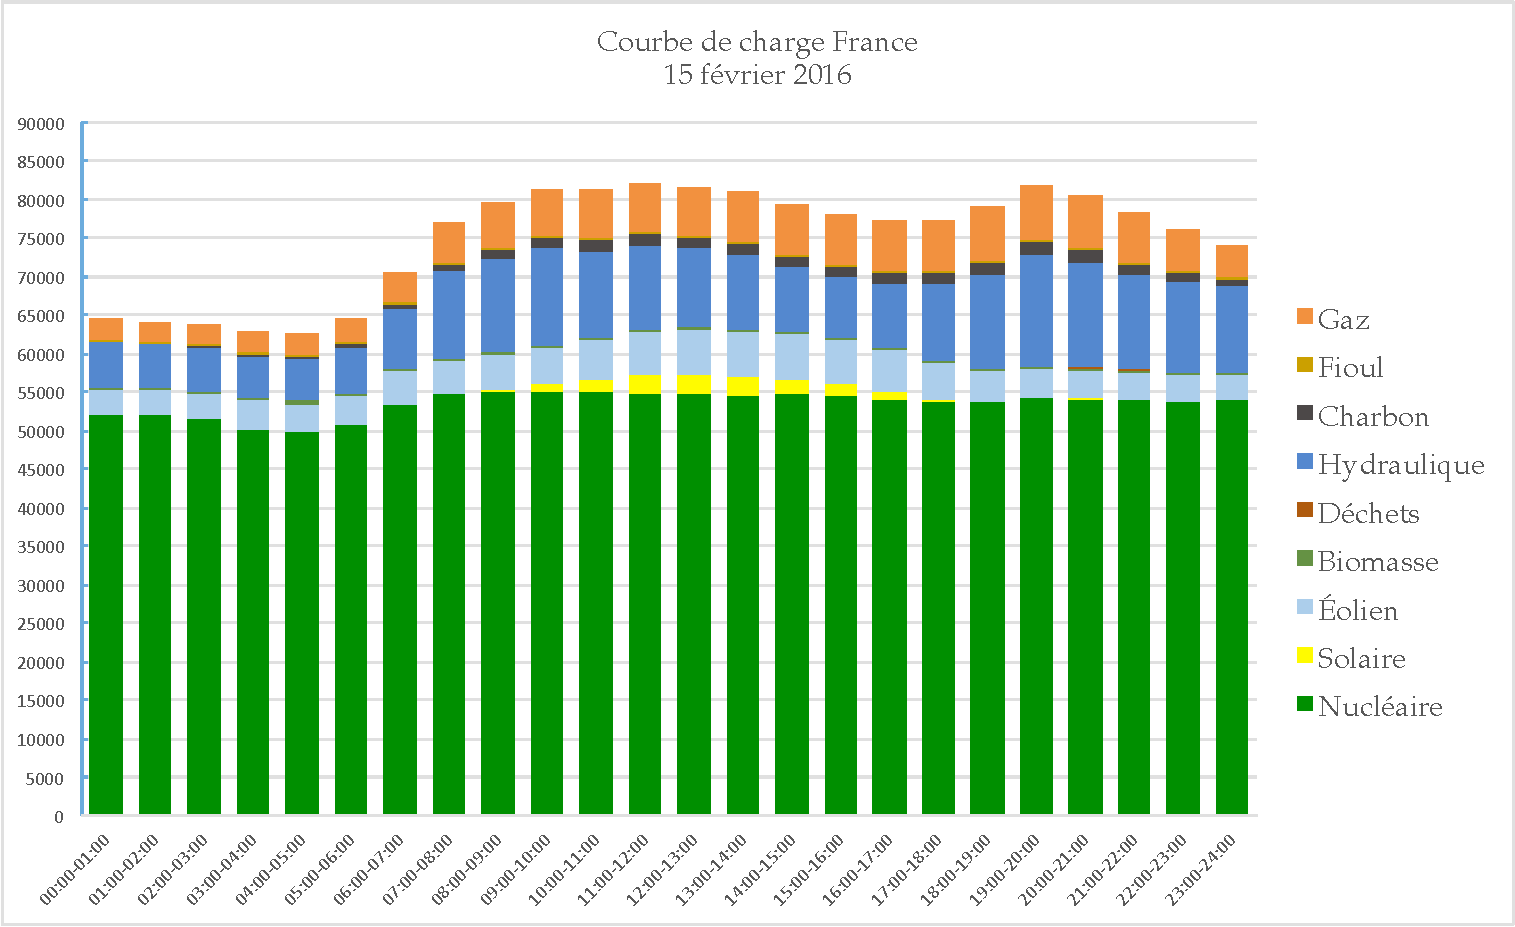
\includegraphics[width=1\textwidth]{figures/1_problematique/courbe_charge.pdf}
 \end{center}
 \caption{Placement du type d'énergie sollicitée sur la courbe de charge 
française du lundi 15 février 2016 (source RTE\protect\footnote{ Réseau Transport France (http://www.rte-france.com/)})}
 \label{fig:courbeCharge}
\end{figure}

Ces pics s'intensifient significativement avec l'émergence de nouveaux usages de 
consommation d'énergie dont, notamment, la mobilité électrique. En France, les 
pouvoirs publics estiment à deux millions le nombre de véhicules électriques en 
circulation en 2020. L'impact de ces véhicules sur l'équilibre entre l'offre et 
la demande n'est pas négligeable. En effet, la recharge complète d'un véhicule 
électrique ayant 150 km d'autonomie est équivalente en termes d'appel de 
puissance à~:
\begin{itemize}[noitemsep]
    \item un chauffe-eau si la recharge s'effectue en 8~h (recharge normale)~;
    \item un immeuble si la recharge s'effectue en 1~h (recharge accélérée)~;
    \item un quartier urbain si la recharge s'effectue en 3~min (recharge rapide).
\end{itemize}



\subsection{Architecture des Smart Grids : \\
vers des réseaux électriques flexibles et communicants}

Pour faire face aux mutations du contexte énergétique, les gestionnaires de 
réseaux électriques ne peuvent plus compter uniquement sur la conduite 
prévisionnelle du réseau électrique (peu réactive face à l'intermittence des 
énergies renouvelables par exemple) ni envisager le redimensionnement du réseau 
(onéreux et non optimal). 

La solution réside dans l'automatisation de la conduite des réseaux électriques, 
grâce a l'acquisition et l'exploitation en temps réel d'informations sur l'état 
des réseaux. Cela passe par le déploiement d'un réseau informatique au niveau 
des infrastructures électriques, et la mise en place dans le \gls{si} d'outils 
pour l'exploiter.

Ainsi équipés, les réseaux électriques s'apparentent à une toile d'araignée où 
les mailles interagissent constamment via des liens de communication. Ces 
mailles correspondent aux acteurs du système électrique~: consommateurs, 
producteurs ou les deux à la fois. Outre l'électricité, ces acteurs produisent 
et consomment de l'information en temps réel grâce aux modules logiciels dont 
ils sont équipés et à divers moyens de télécommunication, tels que les réseaux 
mobiles ou le \gls{cpl}. Ce partage permanent et 
instantané d'informations entre les équipements préserve la stabilité du 
système électrique tout en augmentant son efficacité énergétique.

Pour illustrer les possibilités offertes par les \gls{tic}, prenons l'exemple 
du pic de consommation de la fin de journée d'un jour en semaine. Grâce aux 
\gls{tic}, il devient possible d'agir sur la demande plutôt que sur l'offre. Le
distributeur d'électricité, s'appuyant sur des points de contrôle distants et 
des compteurs intelligents installés chez les clients pour envoyer et recevoir 
des informations et des consignes, peut alors adresser des demandes 
d'effacement aux consommateurs moyennant des incitations tarifaires. Il peut 
s'agir d'une coupure du chauffage pendant 15~min à 30~min d'un foyer ou d'un 
bureau bien isolé. Sans incidence sur le confort des consommateurs, ces 
demandes d'effacement aident à lisser la courbe de charge aux heures de pointe 
tout en évitant de mobiliser des centrales de production. 

Nés de la convergence des réseaux électriques et des \gls{tic}, les Smart Grids 
se composent de trois couches que nous retrouvons dans la figure~\ref{fig:archismartGrids}~:

\begin{enumerate}
    \item le premier niveau correspond à l'infrastructure et aux équipements 
    électriques acheminant l'électricité tels que les lignes et les 
    transformateurs~; 
    \item le second niveau correspond à l'infrastructure de communication 
    composée de différentes technologies de télécommunication comme la fibre 
    optique, le \gls{cpl}, ou encore la \gls{3g}~; 
    \item le troisième niveau correspond aux applications informatiques qui 
    incarnent «~l'intelligence~» du réseau. En utilisant des informations 
    délivrées en temps réel, ces applications calculent des consignes à envoyer 
    aux équipements concernés et automatisent ainsi la conduite du système 
    électrique.  Cette intelligence est centralisée au niveau des centres de 
    conduite du réseau ou distribuée sur les équipements électriques. 
\end{enumerate}

\begin{figure}[!htbp]
  
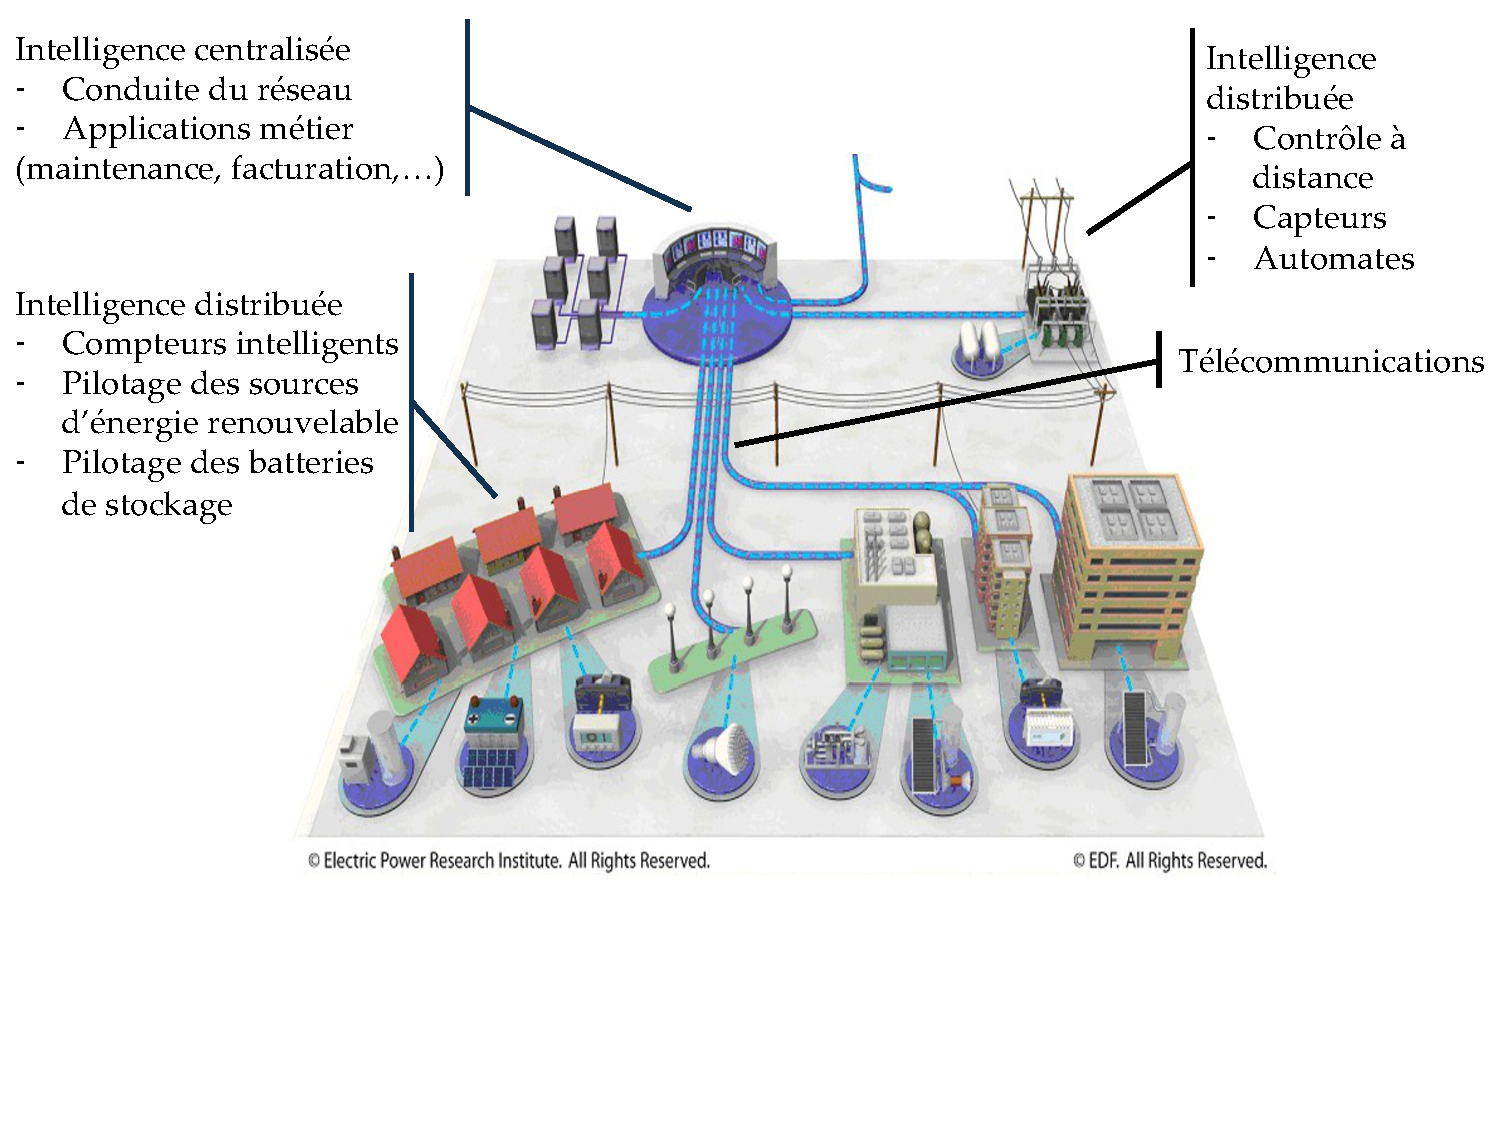
\includegraphics[trim= 0cm 4cm 0cm 0cm, width=1\textwidth]{figures/1_problematique/archiSmartGrids.pdf}
 \caption{Architecture des Smart Grids \protect\cite{favre2006ingenierie}}
 \label{fig:archismartGrids}
\end{figure}


%En effet, la libéralisation du marché de l'électricité exige que le 
%consommateur ait une connaissance en temps réel de l'évolution tarifaire 
%horaire 
%de l'électricité et qu'il puisse même choisir d'injecter sa propre propre 
%production d'énergie sur le réseau.

\section{Problématique industrielle}
%la nécessaire évolution des Systèmes d'Information pour la mise en œuvre d'une stratégie orientée Smart Grids

%Un Smart Grid est un réseau électrique intelligent permettant d'optimiser la 
%production, la distribution et la consommation d'électricité grâce à 
%l'introduction des Technologies de l'Information et de la Communication (TIC) 
%sur le réseau électrique \footnote{www.smartGrids-cre.fr}.

En traitant les données envoyées en temps réel par les capteurs installés sur 
les équipements électriques et chez les consommateurs, les \gls{si} calculent 
des consignes destinées à des organes télécommandés permettant ainsi de piloter 
les 
réseaux électriques à distance. 
Cette automatisation de la gestion des réseaux est une solution pour les adapter 
rapidement face aux contraintes qu'introduit l'intégration des énergies 
renouvelables et des nouveaux usages \cite{cre}. Les \gls{si} sont donc au cœur 
des 
enjeux Smart Grids.  

L'implémentation des Smart Grids va ainsi de pair avec la mise à niveau des 
\gls{si} des gestionnaires du réseau électrique. En effet, ces \gls{si} doivent 
pleinement intégrer les évolutions qu'induisent les Smart Grids au niveau des 
processus 
métier du gestionnaire de réseau, des acteurs impactés, des informations 
échangées ainsi que des applications informatiques et des infrastructures 
techniques sous-jacentes. Parmi ces évolutions nous citons~:

\begin{itemize}
    \item les nouveaux flux d'information provenant du réseau électrique~;

    \item l'entrée en jeu de nouveaux acteurs tels que les producteurs
    décentralisés (éolien, photovoltaïque)~;

    \item les nouveaux équipements communicants comme le compteur Linky 
(\gls{erdf} 
    annonce le déploiement de 30 millions de compteurs d'ici 
    2020\footnote{www.erdf.fr/Linky})~;

    \item les nouvelles réglementations et directives européennes (dans le cas 
    des gestionnaires de réseaux européens)~;

    \item les nouveaux usages comme les véhicules électriques ou encore les 
    maisons connectées.
\end{itemize}

Outre leurs \gls{si}, les gestionnaires de réseaux électriques doivent faire 
évoluer 
leurs stratégies de développement en envisageant de nouveaux modèles métier et 
de nouveaux partenaires, tout en tenant compte de l'émergence des nouvelles 
technologies et des exigences du législateur. Une étude américaine, menée par 
IBM, CISCO, EPRI et South Carolina Edison, fait état de cinq thèmes stratégiques 
clés pour l'implémentation des Smart Grids~:

\begin{itemize}

    \item \textbf{permettre au consommateur de contrôler sa consommation 
    d'énergie} et de réduire son empreinte carbone en utilisant des équipements 
    intelligents et des véhicules électriques et en produisant de l'énergie 
    renouvelable à domicile~;

    \item \textbf{améliorer la sécurité et la productivité des employés} en 
    mettant par exemple à leur disposition des outils performants pour le 
    contrôle à distance, des équipements de protection, et des applications 
    mobiles~; 

    \item \textbf{intégrer des sources d'énergie renouvelables} distribuées sur 
    le réseau en assurant la protection des équipements électriques, le 
    stockage de l'énergie et la stabilité du réseau~; 

    \item \textbf{améliorer l'efficience et la résilience du réseau} à travers 
    les systèmes de mesure en temps réel, l'analyse et le contrôle à distance~;

    \item \textbf{fournir les informations et la connectivité nécessaires} en
    developpant une infrastructure \gls{tic} pour répondre aux besoins 
    d'informatisation du réseau électrique. Ce dernier point est une condition 
    \textit{sine qua non} de la réalisation des quatre précédents.
\end{itemize}

Compte tenu de ces thèmes clés, les gestionnaires de réseaux envisagent des 
stratégies impliquant l'adoption de technologies Smart Grids. 
La mise en œuvre effective de ces stratégies demande l'automatisation des 
actions sur le réseau et du traitement des données, ce qui entraine donc le 
déploiement de nouveaux \gls{si}. Afin d'appréhender ces paradigmes naissants, 
des 
scénarios métier sont élaborés mais il est indispensable de les éprouver et de 
les valider avant d'envisager leur implémentation finale.

Plusieurs démonstrateurs physiques ont été déployés sur le terrain 
\footnote{www.erdf.fr/Carte\_demonstrateurs\_Smart\_Grids}. Ces projets pilotes 
permettent de mener des expérimentations en conditions réelles pour tester des 
fonctions et des services, comme par exemple le démonstrateur InfiniDrive 
\footnote{avem.fr/actualite-erdf-et-le-groupe-la-poste-lancent-le-projet-infini-drive-a-nice-3450.html} 
pour le pilotage des infrastructures de recharge de véhicules électriques ou le 
démonstrateur Venteea \footnote{www.venteea.fr} pour l'intégration d'une forte 
capacité éolienne dans un réseau rural. Cependant, les démonstrateurs 
nécessitent que le gestionnaire de réseau de distribution recrute des clients 
industriels et/ou domestiques qui acceptent d'avoir du matériel à tester chez 
eux. De plus, leur exploitation reste limitée par les réglementations en cours. 
Enfin, leur mise en place se révèle souvent longue et coûteuse. 

En plus de ces démonstrateurs, des réseaux de distribution d'expérimentation 
grandeur nature tel que Concept Grid \footnote{chercheurs.edf.com}, implanté à 
\gls{edf} Lab, permettent de tester les nouveaux équipements avant leur 
installation sur les réseaux du distributeur \gls{erdf}. Ces réseaux ont 
l'avantage de permettre la conduite de \textit{stress tests} en conditions perturbées, 
impossibles à réaliser dans le cadre de démonstrateurs, ceux-ci impliquant de 
vrais clients. Cependant, la taille réduite de ces réseaux reste limitante. 

Pour pallier toutes ces limitations, une troisième voie est la simulation. La 
simulation intègre les trois couches qui composent les Smart Grids~: 
l'infrastructure électrique (transformateurs, lignes, charges, sources), 
l'infrastructure de télécommunication (réseaux mobiles, \gls{cpl}) et enfin les 
\gls{si} qui 
les pilotent. Des simulateurs spécialisés dans la simulation de réseaux 
électriques (EMTP-RV, Dymola, PowerFactory, Eurostag, etc.) ainsi que des 
simulateurs de réseaux de télécommunication (OPNET, NS-3, OMNeT ++, etc.) ont 
déjà validé l'apport de la simulation dans leurs domaines respectifs. Toutefois, 
les \gls{si} sont souvent relégués à de simples modèles de calcul de consignes 
souvent 
développés en Matlab ou en C++ \cite{palensky2014simulating}. 

Dans ce contexte, la problématique industrielle dans laquelle  s'inscrivent nos 
travaux de recherche est donc la suivante~: 

\textbf{Comment valider une stratégie de développement orientée Smart Grids à 
travers la simulation de sa déclinaison au niveau du SI du gestionnaire du 
réseau électrique~?}

 
\section{Problématique de recherche}

%\subsection{Le recours à l'Architecture d'Entreprise}

Les technologies Smart Grids illustrent le défi que représente l'évolution des 
\gls{tic} et l'intégration des énergies renouvelables pour les gestionnaires de 
réseaux électriques. Jeremy Rifkin annonce même «~une troisième révolution 
industrielle, fondée sur le couplage des technologies de l’Internet et des 
énergies nouvelles~» \cite{rifkin2012troisieme}. 

Mais à l'ère numérique, l'adaptation au changement relève des préoccupations de 
toute entreprise s'appuyant sur les \gls{tic} pour mener ses 
activités. Le très haut niveau de concurrence que connait le secteur des 
technologies de l'information stimule l'innovation. Or ces technologies sont de 
plus en plus le moteur qui fait progresser les  métiers de l'entreprise. Être 
capable de s'adapter continuellement à l'évolution rapide et 
constante des \gls{tic} représente donc un véritable challenge pour les 
entreprises 
d'aujourd'hui.

Pour mener à bien tout changement, il est primordial de commencer par une 
description représentative de «~l'objet~» à changer, qu'il s'agisse d'une 
nouvelle version d'un avion, d'une voiture, d'un ordinateur ou encore d'une 
entreprise \cite{zachman1997enterprise}. Cette description représentative 
revient à concevoir l'architecture de l'objet en question. L'architecture en 
tant qu'activité est centrale dans plusieurs disciplines, allant de 
l'architecture du bâtiment à l'architecture logicielle, en ce qu'elle est un 
outil indispensable à la construction d'artefacts respectant les qualités 
attendues de l'objet final. En précurseur, Zachman \cite{zachman1997enterprise} 
recommande d'appliquer les principes d'architecture à l'entreprise pour faire 
face aux changements dictés par l'innovation technologique.

Les \gls{si} sont en première ligne dès qu'il s'agit de l'évolution des 
\gls{tic}. Nos 
travaux se sont donc d'abord portés sur l'évaluation de l'impact de cette 
évolution sur les \gls{si} de l'entreprise. De ce fait, nous nous sommes d'abord 
appliqués à décrire l'architecture de ces \gls{si} \cite{seghiri2015simulation}. 

Les changements apportés par ces technologies impactent cependant, non seulement 
les \gls{si}, mais l'entreprise dans son ensemble~: de sa stratégie à ses 
partenaires, en passant par ses objectifs, ses clients et ses processus métier. 
Par exemple, 
l'utilisation des véhicules électriques fait évoluer le \gls{si} du 
gestionnaire du réseau électrique qui doit mettre en place de nouvelles 
applications capables de bien gérer leur recharge. Mais il doit aussi faire 
évoluer son modèle métier en mettant à disposition de nouveaux contrats 
client favorisant la recharge hors de la période des pics de consommation par exemple, 
ou encore créer de nouveaux partenariats avec les constructeurs 
automobiles comme dans le cas d'\gls{edf} et Renault-Nissan qui collaborent sur 
un système de recharge pour véhicule électrique permettant à ce dernier de 
communiquer avec les bornes de recharge.

Évaluer l'adoption de nouvelles technologies de l'information oblige à prendre 
en compte l'entreprise dans son ensemble afin de garantir une cohérence entre 
la stratégie d'évolution adoptée et les \gls{si} qui implémentent cette 
stratégie. Parce que l'alignement entre la stratégie métier et le \gls{si} est 
au cœur de l'\gls{ea}\footnote{L'acronyme EA (\textit{Enterprise Architecture}) 
est souvent utilisé même dans la communauté francophone.} 
\cite{zachman1997enterprise}, nous
adoptons l'\gls{ea} pour évaluer l'impact des technologies Smart Grids sur les
gestionnaires des réseaux électriques. Il est en effet indispensable de
concevoir une architecture cible pour avoir  «~une vision générale de comment
une entreprise va mettre en œuvre sa stratégie~» \cite{ross2006enterprise}.

L'\gls{ea} participe à l'alignement des composants d'une entreprise en offrant 
une vision globale et transverse \cite{zachman1987framework}. Dans le contexte 
des 
Smart Grids par exemple, elle permet d'aligner efficacement les intérêts des 
acteurs impliqués dans leur implémentation tels que les experts métier, les 
conseillers stratégiques, les experts environnementaux ou encore les experts en 
normalisation.

L'exécution effective d'une stratégie est cependant confrontée à des barrières 
de communication au sein de l'entreprise \cite{vcater2010factors}. Le recours à 
l'\gls{ea} est d'autant plus justifié qu'elle représente un outil pour la 
transmission des objectifs stratégiques à tous les niveaux hiérarchiques de 
l'organisation en 
question \cite{kappelman2008enterprise}. 

Pour toutes ces raisons, nous souhaitons mettre à profit les principes 
d'\gls{ea} pour évaluer l'impact de l'adoption des technologies Smart Grids sur 
les \gls{si} des 
gestionnaires de réseaux électriques, tout en garantissant la cohérence entre la 
stratégie adoptée et les \gls{si} qui les implémentent. 

%\cite{buckl2010conceptual}. Le recours à l'architecture d'entreprise est ainsi 
%pleinement justifié.

%\subsection{Le recours à la simulation}

Les Smart Grids correspondent à des systèmes dynamiques et complexes 
\cite{monti_power_2010} étant donné le grand nombre de parties prenantes qui 
interagissent eux (tels que les producteurs d'énergie renouvelable ou les 
consommateurs actifs sur le réseau), tout en ayant des comportements autonomes 
et des objectifs différents. Les \gls{si} pilotant les  Smart Grids 
correspondent par conséquent à des systèmes dynamiques aux comportements 
complexes. Borshchev et 
Filippov\cite{borshchev2004system} affirment que le seul moyen d'adresser cette 
complexité est de simuler ces systèmes. La simulation est une technique connue 
pour valider ou critiquer la conception d'un système dès les premières étapes 
de son cycle de développement. Les acteurs impliqués dans le déploiement des 
Smart Grids acquièrent, par la  simulation, une connaissance approfondie et 
directe des modèles créés pour valider ou critiquer leur choix d'implémentation.

Néanmoins, les approches d'\gls{ea} se focalisent le plus souvent sur des 
aspects statiques et structurels tels que les interconnexions entre les 
différentes applications métier \cite{buckl2008towards}. De plus, les modèles 
issus de ces 
approches sont ne sont pas exécutables et sont conçus en 
priorité pour la documentation et la communication entre parties prenantes 
\cite{kulkarni2013modelling}. Notre problématique de recherche se résume de ce 
fait dans la question suivante :

\vspace*{1em}
\begin{framed}
{\bfseries Quels méthodes, modèles et outils adopter pour simuler une 
architecture d'entreprise afin de la valider?}
\end{framed}





    %!TEX  root = main.tex
\chapter{Architecture d'Entreprise}
\label{ch:EA}

\PartialToc

\vspace*{2em}
L'émergence des Smart Grids suscitent de profonds changements
non seulement au niveau réseaux électriques et les
SI qui les pilotent mais pour l'ensemble de l'entreprise qui fournit et distribue de l'électricité~:
sa stratégie de développement, ses processus métier, etc. L'EA a pour objectif d'accompagner
ce type de changements en capturant les différents composants de l'entreprise et leurs relations. C'est à ce
titre que notre état de l'art traite de l'EA.

Ce chapitre présente ainsi les notions fondamentales de l'EA dans la section~\ref{sec:notions_EA} avant 
de présenter les principes guidant la conception d'une architecture d'entreprise
dans la section~\ref{sec:conception_EA}. L'objectif de ces travaux de thèse étant de valider
les évolutions envisagées pour une architecture d'entreprise avant leur implémentation, nous
considérons, dans la section~\ref{sec:analyse_EA}, les approches
d'analyses existantes.




\section{Notions fondamentales de l'Architecture d'Entreprise}
\label{sec:notions_EA}

% Comme précédemment exposé dans notre problématique de recherche (cf. chapitre 
% \ref{ch:problematique}), nos travaux se sont d'abord portés sur la modélisation 
% et la simulation du SI des Smart Grids. Cependant, le SI est sensé répondre de 
% manière pertinente aux besoins de l'entreprise et implémenter efficacement sa 
% stratégie. Avant toute simulation, nous devons donc de facto prendre en compte 
% la stratégie de l'entreprise et ses objectifs métier et la mettre en cohérence 
% avec le SI qui l'implémente.




% L'alignement métier/SI est au cœur de l'EA, une discipline à part entière qui 
% traite le SI en le corrélant au reste de l'entreprise. En effet, l'EA offre une 
% vision globale des composants de l'entreprise tels que les processus métier, les 
% parties prenantes, les informations, les fonctions, les applications 
% informatiques, les infrastructures techniques. 
 
\subsection{Terminologie}

Pour cette première partie de l'état de l'art consacré à l'EA, nous commençons 
par définir les termes de SI et d'EA. 
	
\subsubsection{Système d'Information}
\label{sec:reix}

Une définition communément admise du SI est donnée par Robert Reix~\cite{reix1995systemes}:
\\
\begin{definition}
Le SI est un ensemble organisé de ressources : matériel, 
logiciel, personnel, données, procédures permettant d'acquérir, de traiter, de 
stocker des informations (sous forme de donnée, textes, images, sons, etc.) dans 
et entre des organisations
\end{definition}

Nous adoptons cette définition car elle a l'avantage de ne pas réduire le SI 
d'une organisation à son système informatique. Le système informatique est 
constitué de l'ensemble du patrimoine matériel (hardware) et applicatif 
(software) de la dite 
organisation et a pour objectif d'automatiser le traitement de l'information. 
Nous adoptons l'acronyme IT (\textit{Information Technologies}) pour le 
différencier du SI.

On suppose souvent que les SI sont totalement informatisés et c'est une des 
raisons qui mènent à confondre SI et \ Cependant, le SI comprend non seulement 
le système informatique mais aussi des ressources humaines telles que les 
partenaires ou le personnel et des ressources matérielles comme les procédures 
de gestion ou encore le savoir-faire métier.

\subsubsection{Architecture d'Entreprise}

Il existe une multitude de définitions de la notion  l'architecture d'entreprise. Nous
rapportons ici celle donnée par Zachman~\cite{zachman1997enterprise}, fondateur de l'EA. 
\\
\begin{definition}
Une architecture d'entreprise est un ensemble pertinent 
d'artefacts de conception ou de représentations descriptives pour décrire une 
entreprise de manière à ce cette entreprise soit créée en respectant certaines 
exigences et à ce qu'elle soit facilement maintenue tout au long de son cycle de 
vie. 
\end{definition}

Zachman voit ainsi dans l'architecture un gage de qualité et de maintenabilité. 
L'EA revient à appliquer à l'entreprise les principes de l'architecture telle 
qu'elle est pratiquée dans de nombreuses autres disciplines comme par exemple 
l'architecture du bâtiment. Construire une maison en procédant chambre par 
chambre sans plan d'architecture général peut en effet mener à un résultat peu 
probant. De même, le développement préalable d'une organisation sans 
architecture de référence risque de mener à une duplication de ses ressources et 
altère par conséquent son efficacité, sa cohérence interne rend fastidieuse 
toute entreprise de changement~\cite{zachman1997enterprise} 
\cite{bernard2012introduction}. 

Il est important de noter que le terme architecture d'entreprise peut prêter à 
confusion car il est à la fois utilisé pour désigner (1) l'activité de 
conception d'une architecture i.e., la description des éléments composant 
l'organisation en question et leurs relations mais aussi (2) l'ensemble des 
artefacts résultant de cette activité. Pour éviter toute confusion, nous 
désignons l'activité de conception par l'acronyme EA et le résultat de cette 
activité, c'est-à-dire les artefacts qui en sont issus, comme étant 
l'architecture de l'entreprise. L'EA est apparue en tant que discipline dans 
les années 1980 suite à l'informatisation accrue des entreprises mais son 
périmètre ne cesse d'évoluer depuis. La section suivante écrit les raisons et 
les grandes étapes de cette évolution. 

%%S'agissant du terme «~entrerprise~», Scott Bernard 
%\cite{bernard2012introduction} y réfère comme une organisation ou une 
%sous-partie d'une organisation qui poursuit des objectifs 
%%communs, en s'appuyant sur les mêmes processus et en utilisant les mêmes 
%%ressources. Une entreprise peut être publique ou privée, avoir ou pas un but 
%lucratif. 

\subsection{Évolution de l'Architecture d'Entreprise}

L'EA est ancrée dans l'architecture de systèmes informatiques
\cite{kappelman2008enterprise}. Mais le périmètre de l'EA ne cesse de s'étendre
en comprenant d'abord l'IT et certains aspects métier de l'entreprise
\cite{winter2006essential}, évoluant ensuite en adressant l'ensemble de
l'entreprise en intégrant sa stratégie et ses processus décisionnels
\cite{ross2006enterprise}, et allant même jusqu'à aborder l'environnement dans
lequel elle évolue \cite{lapalme2012three}.

L'origine de l'EA\footnote{D'après Scott Bernard
\cite{bernard2012introduction}, le terme Architecture d'Entreprise a fait sa
première apparition dans le livre de Steven Spewak intitulé «~Enterprise
Architecture Planning~: developping a blueprint for data, applications and
technology~» \cite{spewak1993enterprise}.} remonte en effet aux travaux de
Zachman, souvent considérés comme précurseurs.  Il y propose un cadre
d'architecture pour l'IT \cite{zachman1987framework} afin d'optimiser la
gestion du patrimoine applicatif et de l'infrastructure technique de
l'entreprise. À ses débuts, l'EA se focalise donc sur des artefacts purement IT
(data, logiciels, équipements) pour rationaliser l'utilisation des ressources
informatiques \cite{winter2006essential}, tout en répondant aux besoins métier
de l'entreprise. L'EA est alors guidée par les pratiques de l'ingénierie
logicielle. 

Cependant, l'accroissement de la complexité de l'IT et son rôle de plus en plus
prégnant dans le cœur de métier des entreprises
\cite{ranganathan2005enterprise} ont fait de l'architecture IT une
problématique inhérente à l'ensemble des composants de l'entreprise. Pour y
faire face, l'EA a commencé à inclure quelques aspects métier tels les
processus les acteurs impliqués \cite{winter2006essential}. En intégrant ainsi
des problématiques métier, l'EA ne relève plus de l'architecture IT mais de
l'architecture du SI dans son ensemble.

Pour Scott Bernard, l'EA doit même aller plus loin en intégrant la stratégie de
l'entreprise dans son périmètre pour offrir une vision globale de l'ensemble
des ressources de l'entreprise \cite{bernard2012introduction}. Le terme
«~entreprise~» implique ainsi une vue à haut niveau de l'ensemble de
l'organisation. Le terme «~architecture~» fait référence à la mise en place
d'un cadre structuré et cohérent pour l'analyse, le planning, et le
l'exploitation de toutes les ressources dont dispose l'entreprise pour
atteindre ses objectifs.  

Enfin, certains auteurs insistent sur le fait que l'entreprise évolue dans un
environnement inconstant \cite{lapalme2012three}. L'EA doit par conséquence
inclure les relations de l'entreprise avec son environnement pour mesurer
l'impact de ce dernier et faciliter les processus d'adaptation et d'innovation.
Les différentes phases d'évolution de l'EA sont à l'origine de l'apparition de
plusieurs écoles que nous détaillons dans la section suivante. 


\subsection{Écoles de pensée de l'Architecture d'Entreprise} 
\label{Lapalme}

Aucune définition de l'EA n'a été universellement adoptée
\cite{mentz2012comparison} \cite{ranganathan2005enterprise}. Il existe en effet
une pléiade de définitions émanant aussi bien du milieu académique que du
milieu industriel donnant ainsi lieu à plusieurs écoles de pensée. Ce manque de
consensus est du à la nature intrinsèque de l'activité d'EA~:~celle-ci est
régie par un ensemble de préceptes et de bonnes pratiques que l'architecte
reste libre d'adapter au contexte de l'entreprise.
Il est toutefois possible d'identifier un thème commun à toutes les définitions
proposées~ \cite{lapalme2012three}: 
\\
\begin{definition}
L'architecture d'entreprise décrit les composants interdépendants
d'une organisation et guide leurs évolutions. 
\end{definition}


En revanche, le \textit{périmètre} de cette description ainsi que les
\textit{préoccupations} adressées diffèrent d'une définition à l'autre.

S'agissant du \textit{périmètre}, le terme «~entreprise~» peut couvrir
uniquement l'IT ou s'étendre à tous ses composants humains, stratégiques,
économiques et techniques. Les \textit{préoccupations} sous-jacentes à l'EA
peuvent quant à elles couvrir des objectifs allant de l'optimisation des
investissements dans l'infrastructure technique à l'implémentation de la
stratégie de l'entreprise en passant par l'alignement métier/IT. 

Partant de ce constat, James Lapalme identifie trois écoles de pensée en EA 
\cite{lapalme2012three}~:~l'architecture de l'IT d'entreprise 
(\textit{Enterprise IT Architecting}), l'architecture intégrative de 
l'entreprise 
(\textit{Enterprise Integrating}) et l'architecture de l'entreprise dans son 
environnement (\textit{Enterprise Ecological Adaptation}). Chaque école a son 
propre système de croyance (devise, préoccupations et objectifs, principes et 
postulats).


%\textcolor{red}{Le terme "système de croyances" est vraisemblablement emprunté 
%à la sociologie, j'aime bien l'idée d'utiliser d'autres disciplines pas 
%forcément directement mais Lapalme ne fait pas du tout la référence à la 
%sociologie en parlant de belief system. J'ai une amie qui a un master en socio 
%je peux lui demander une petite référence pour définir exactement ce qu'est un 
%système de croyances. En lisant la préface de Zachman dans le livre de Scott 
%Bernard, on y 
%entrevoit clairement une problématique de catégorie de gens qui croient que la 
%clé de l'architecture c'est la technologie sans tenir compte des 
%problématiques métier. à voir donc. Au pire je supprime simplement le terme 
%«~système de croyances~» mais je trouve ça dommage parce que ça explique pas 
%mal 
%de choses.}

Il est important de noter que cette catégorisation est épurée voire
idéalisée, dans la mesure où le majorité des auteurs gravitent autour d'une
école plutôt que de se conformer complètement à une seule école.
\textit{Enterprise IT Architecting} réduit le périmètre de l'architecture à
l'IT de l'entreprise.  \textit{Enterprise Integration} adopte une approche
intégrative en incluant toute l'entreprise dans son périmètre, de sa stratégie
métier à la gestion de son patrimoine applicatif. \textit{Enterprise Ecological
Adaptation} inclue l'environnement dans lequel évolue l'entreprise pour en
déterminer les impacts potentiels et mettre en place une stratégie d'adaptation
adéquate. Le tableau \ref{tab:ecolePensee} résume ces écoles de pensée en
termes de devises, objectifs et principes. 

\begin{table}[!ht]
	\setlength{\mytablewidth}{1.1\textwidth}
\setlength{\dashlinedash}{0.5pt}
\setlength{\dashlinegap}{1pt}
\setlength{\arrayrulewidth}{0.5pt}
\begin{adjustbox}{width=\mytablewidth,center}
    \setlength{\mycolwidth}{\dimexpr0.28\mytablewidth-2\tabcolsep\relax}
    \setlength{\myfirstcolwidth}{\dimexpr0.16\mytablewidth-2\tabcolsep\relax}
    \scriptsize
    \begin{tabulary}{\mytablewidth}{@{}>{\bfseries}p{\myfirstcolwidth}p{\mycolwidth}p{\mycolwidth}p{\mycolwidth}@{}}
        %  --------------------------------------------------------------------
        \toprule
        & \centering\textbf{Enterprise IT Architecting} \
        & \centering\textbf{Enterprise Integration} \
		& \centering\textbf{Enterprise Ecological\newline Adaptation}\
        \tabularnewline\midrule
        %  --------------------------------------------------------------------
        \multirow{1}{\myfirstcolwidth}{Devise} \
        & L'architecture d'entreprise raccorde l'IT au métier de l'entreprise \
        & L'architecture d'entreprise lie la stratégie et son exécution \
        & L'architecture d'entreprise est un moyen d'innovation organisationnelle et une garantie de durabilité  \
        \tabularnewline\midrule
        %  --------------------------------------------------------------------
        \multirow{3}{\myfirstcolwidth}{Objectifs et préoccupations} \
        & Planifier l'IT et en optimiser les coûts \
        & Implémenter efficacement la stratégie de l'entreprise \
        & Adapter et innover \
        \tabularnewline\addlinespace\cdashline{2-4}\addlinespace%\tabularnewline\cmidrule{2-4}
        & Appuyer le métier \
        & Assurer la cohésion de l'organisation \
        & Assurer la cohésion de l'organisation \\
        \tabularnewline\addlinespace\cdashline{2-4}\addlinespace%\tabularnewline\cmidrule{2-4}
        & \
        & \
        & Encourager la co-évolution entre l'entreprise et son environnement \
        \tabularnewline\midrule
        %  --------------------------------------------------------------------
        \multirow{4}{\myfirstcolwidth}[4pt]{Principes et postulats} \
        & Appliquer une approche réductionniste \
        & Appliquer une approche holistique \
        & Appliquer une approche holistique \
        \tabularnewline\addlinespace\cdashline{2-4}\addlinespace%\tabularnewline\cmidrule{2-4}
        & Ne pas remettre en question la stratégie et les objectifs métier \
        & Ne pas remettre en question la stratégie et les objectifs métier \
        & Créer la stratégie de l'entreprise est une priorité \
        \tabularnewline\addlinespace\cdashline{2-4}\addlinespace%\tabularnewline\cmidrule{2-4}
        & Concevoir les composants de l'organisation de manière indépendante \
        & Concevoir les différents aspects de l'entreprise de manière intégrative\
        & Concevoir les différents aspects de l'entreprise de manière intégrative\
        \tabularnewline\addlinespace\cdashline{2-4}\addlinespace%\tabularnewline\cmidrule{2-4}
        & Ne pas se préoccuper des aspects non IT \
        & Tenir compte de l'environnement comme source de changement \
        & L'environnement peut être transformé \
        \tabularnewline\midrule
    \end{tabulary}
\end{adjustbox}
	
	\caption{Écoles de pensée de l'Architecture d'Entrerpise selon
\protect\cite{lapalme2012three}}
 	\label{tab:ecolePensee}
\end{table}

En définissant sa taxonomie, Lapalme insiste sur le fait que ces écoles de
pensée se sont formées par héritage~:~l'\textit{Enterprise Ecological
Adaptation} hérite de l'\textit{Enterprise Integration}, qui elle-même hérite
l'\textit{Enterprise IT architecting}. Cependant, cet l'héritage implique une
transcendance car il existe des différences fondamentales entre ces trois
écoles de pensée. Par exemple, l'approche réductionniste de
l'\textit{Enterprise IT architecting} est fondamentalement opposée à l'approche
holistique des deux autres écoles. Mais quelle qu'en soit l'école de pensée,
l'EA présente des avantages certains pour l'entreprise que nous rapportons dans
la section suivante. 


%\textcolor{red}{Peut être que c'est là que je positionne les travaux par 
%rapport aux écoles de pensée. Ou alors je le fais dans la partie démarche en y 
%dédiant une section "positionnement" ? Ce que je veux dire c'est que nous on 
%essaie de prendre en compte la stratégie voire même de l'évaluer par 
%simulation.}

\subsection{Avantages de l'Architecture d'Entreprise}

L'EA organise et structure les informations à l'échelle de l'entreprise tout en
fournissant les détails appropriés à chacune des parties prenantes et en
définissant le schéma directeur nécessaire à la construction de SI évolutifs et
pertinents pour le métier. 

%Avec l'avènement de l'économique numérique, l'EA est autant indispensable au 
%succès d'une entreprise que son IT 

Pour Zachman, manier l'architecture de l'entreprise avec agilité et l'adapter
rapidement à un contexte économique et technologique en constante évolution est
un facteur de survie déterminant pour les entreprises du 21\up{ème} siècle
\cite{zachman1997enterprise}. Afin de souligner l'importance de l'EA, Ross
\cite{rossyoutube} donne l'exemple d'une problématique d'architecture que
l'entreprise américaine \textit{Jonhson\&Johnson} a rencontré en 1995. Le
succès international de cette entreprise repose surtout sur l'autonomie de ses
170 filiales. Ses managers sont parfaitement satisfaits des processus métier
mis en place mais ce n'est pas le cas de tous ses clients. Les très grands
clients reçoivent en effet de nombreux bons de commande et plusieurs factures
des différentes filiales de \textit{Johnson\&Johnson} et doivent donc les
traiter séparément.  Ces clients exigent un jour de ne recevoir qu'une seule
facture. Or \textit{Johnson\&Johnson} n'en est pas capable. Ni ses processus
métier, ni sa structure organisationnelle et encore moins son IT ne lui permet
d'accéder à la demande de ses clients. Ceci est un cas d'école typique que
permet d'adresser l'EA.

L'EA présente plusieurs avantages liés autant aux aspects purement IT qu'aux
aspects métier. D'abord, en capturant l'essence du métier, de l'IT et de son
évolution \cite{lankhorst2013enterprise}, l'EA permet d'abstraire la
complexité d'un système telle qu'une entreprise. Ensuite, en tant que
référentiel et support de communication, l'EA facilite la coordination entre les
projets IT d'une entreprise, la supervision des ressources techniques ainsi que
la suppression des redondances applicatives \cite{shah2007frameworks}. Enfin,
l'EA est un moyen efficace pour représenter les composants d'une entreprise
dans son état courant et désiré. Comme tableau de bord, l'EA facilite l'accès à
l'information nécessaire à l'optimisation des processus métier et à
l'alignement effectif entre l'IT et la stratégie adoptée. 

\section{Conception d'une architecture d'entreprise}
\label{sec:conception_EA}

L'EA peut faciliter le processus de prise de décision si elle aboutit à une
vision à la fois globale et adaptée aux décideurs. Dans la section suivante, nous
présentons quelques approches et cadres d'EA prenant en compte le processus de
prise de décision et les acteurs qu'il implique.

\subsection{Approches orientées points de vue}

Quelle qu'en soit l'école, l'EA reste une tâche complexe
\cite{steen2004supporting} car elle implique un grand nombre de parties
prenantes. Chaque partie prenante a des préoccupations et des systèmes de
notation propres et relatifs à son domaine d'expertise et aux responsabilités lui
incombant.

L'EA doit capturer une grande variété de composants difficiles à représenter
dans un seul et unique modèle. En procédant par analogie avec l'architecture
d'une vile, la multitudes d'acteurs concernés peuvent difficilement lire un plan où l'on
représente à la fois les rues et les bâtiments ainsi que les réseaux de
transports, d'électricité, de gaz et d'eau. 

Il en va de même pour l'architecture d'entreprise. La nature mutli-facettes
inhérente à l'entreprise rend inappropriée toute approche monolithique
\cite{armour1999bigpicture}. En effet, un analyste métier est concerné par les
processus et les fonctions métier tandis qu'un administrateur de bases de
données est concerné par les données manipulées. Pour cette raison, la plupart des
cadres d'EA adoptent une approche par points de vue.

Les approches orientées points de vue sont d'abord utilisées pour la
spécification des besoins en ingénierie logicielle \cite{mullery1979core}. Les
chercheurs s'intéressent alors aux systèmes à «~perspectives multiples~»
\cite{finkelstein1992viewpoints} \cite{kotonya1996requirements}
\cite{nuseibeh1994multi} \cite{meyers1993representing}. Ces travaux précurseurs
contribuent à l'émergence de plusieurs normes pour les systèmes logiciels,
proposant des cadres d'architecture orientés points de vue. C'est le cas de la
norme IEEE-1471 \cite{hilliard2000ieee}, du standard \gls{rmodp}
\cite{raymond1995reference} ou encore du standard MDA (\textit{Model Driven
Architecture}) \cite{kleppe2003mda}.

Dans la norme IEEE\-1471 \cite{hilliard2000ieee}, une vue correspond à une
représentation du système selon une certaine perspective à laquelle est
associé un ensemble de préoccupations. Les vues permettent ainsi de séparer
les préoccupations des différentes parties prenantes. Un point de vue
correspond, quant à lui, à un \textit{template} pour la création de vues. Il formalise
les objectifs des parties prenantes concernées par la vue ainsi que les
techniques qui permettent de la créer et de l'analyser. Pour décrire un point
de vue, la norme IEEE\-1471 \cite{hilliard2000ieee} exige de spécifier les
attributs suivants~:
\begin{itemize} 
	\item le nom du point de vue~;
	\item la partie prenante ciblée~;
	\item les préoccupations de celle-ci~;
	\item le langage, les techniques de modélisation ou encore les méthodes d'analyse à utiliser pour
la création de la vue. 
\end{itemize}

\subsection{Cadres d'Architecture d'Entreprise}

Les approches orientées points de vue sont largement utilisées en ingénierie
logicielle comme moyen d'adresser la complexité des architectures
\cite{steen2004supporting}. Comme l'EA trouve ses racines dans l'architecture
IT \cite{winter2008enterprise}, de nombreux cadres d'EA recourent aux points de
vue en transférant les concepts développés pour architecture IT à l'EA. Parmi
les cadres d'EA les plus utilisés nous citons le cadre Zachman, \gls{togaf}. Nous citons aussi d'autres cadres d'architecture spécifiques à leurs domaines comme \gls{rmodp} et \gls{sgam}. 

\subsubsection{Le cadre Zachman}

Zachman \cite{zachman1987framework} propose de structurer et d'organiser les
différentes représentations intervenant dans la description d'une entreprise en
les classant selon une matrice à deux dimensions. La dimension verticale
correspond aux points de vue et la dimension horizontale aux abstractions.
Comme l'illustre le tableau~\ref{fig:Zachman}, chaque cellule de la matrice
correspond à l'intersection entre une partie prenante impliquée dans le
processus de conception de l'architecture et une abstraction présentée sous
forme d'une question. Chaque représentation est alors adaptée aux acteurs
impliqués. 

%Le cadre Zachman demande ainsi de spécifier~:
%\begin{description}
%
%    \item[la dimension verticale], divisée en six points de vue qui sont le
%    Planificateur, le Propriétaire, le Concepteur, le Réalisateur et le
%    Sous-traitant \textit{(visionary, owner, designer, builder,
%    implementer)})~;
%
%    \item[la dimension horizontale], divisée en six abstractions qui
%    correspondent au Quoi, Comment, Qui, Quand, et Pourquoi \textit{(What, How,
%    Who, When, Why)}.
%
%\end{description}

\begin{table}[!ht]
    \vspace*{0.4cm}
    % Resources:
% Arrows: http://tex.stackexchange.com/a/60627/32098
% Rotating tikz label: http://tex.stackexchange.com/a/115565/32098

% HACK (and an ugly one) since booktabs breaks vertical separators, we use tikz
% to draw them. Alignment is pretty much custom. I just hope this is gonna work
% with no adjusment when putting this in the main document.
\setlength{\mytablewidth}{\textwidth}
\setlength{\myfirstcolwidth}{\dimexpr0.2\mytablewidth-2\tabcolsep\relax}
\setlength{\mycolwidth}{\dimexpr0.17\mytablewidth-2\tabcolsep\relax}
\newcommand\mycell[1]{{\tiny{#1}}}

\begin{adjustbox}{width=\mytablewidth,center}
    \scriptsize
    \noindent\begin{tabulary}{\mytablewidth}{m{\myfirstcolwidth}m{\mycolwidth}m{\mycolwidth}m{\mycolwidth}m{\mycolwidth}m{\mycolwidth}}

        % \cmidrule[\heavyrulewidth]{2-6}
        \multirow{2}{*}{}\tikzmark{zachmantopleft} \
        & \centbf{Données} \
        & \centbf{Fonctions} \
        & \centbf{Personnel} \
        & \centbf{Temps} \
        & \centbf{Motivation}\tikzmark{zachmantopright} \
        \tabularnewline
        & \centit{Quoi} \
        & \centit{Comment} \
        & \centit{Qui} \
        & \centit{Quand} \
        & \centit{Pourquoi} \
        \tabularnewline\midrule

        \tikzmark{zachmanlefttop}\textbf{Exécutif}\newline\textit{Planification} \
        & {\tiny{Identification\newline des données}} \
        & {\tiny{Identification\newline des processus}} \
        & {\tiny{Identification\newline des responsabilités}} \
        & {\tiny{Identification\newline des échéances}} \
        & {\tiny{Identification\newline des motivations}} \
        \tabularnewline\midrule

        \textbf{Management}\newline\textit{Définition} \
        & {\tiny{Définition\newline des données}} \
        & {\tiny{Définition\newline des processus}} \
        & {\tiny{Définition\newline des responsabilités}} \
        & {\tiny{Définition\newline des échéances}} \
        & {\tiny{Définition\newline des motivations}} \
        \tabularnewline\midrule

        \textbf{Architecte}\newline\textit{Conception}  \
        & {\tiny{Conception\newline des données}} \
        & {\tiny{Conception\newline des processus}} \
        & {\tiny{Conception\newline des responsabilités}} \
        & {\tiny{Conception\newline des échéances}} \
        & {\tiny{Conception\newline des motivations}} \
        \tabularnewline\midrule

        \textbf{Ingénieur}\newline\textit{Spécification} \
        & {\tiny{Spécification\newline des données}} \
        & {\tiny{Spécification\newline des processus}} \
        & {\tiny{Spécification\newline des responsabilités}} \
        & {\tiny{Spécification\newline des échéances}} \
        & {\tiny{Spécification \newlinedes motivations}} \
        \tabularnewline\midrule

        \tikzmark{zachmanleftbottom}\textbf{Technicien}\newline\textit{Implémentation} \
        & {\tiny{Implémentation\newline des données}} \
        & {\tiny{Implémentation\newline des processus}} \
        & {\tiny{Implémentation\newline des responsabilités}} \
        & {\tiny{Implémentation\newline des échéances}} \
        & {\tiny{Implémentation\newline des motivations}} \
        \tabularnewline\bottomrule
    \end{tabulary}
    \begin{tikzpicture}[overlay,remember picture]

        % top horizontal arrow
        \draw[<->] let \p1=(zachmantopleft), \p2=(zachmantopright) in ($(\x1,\y1)+(1.6,0.4)$) -- node[label=Abstractions (colonnes)] {} ($(\x2,\y2)+(0.4,0.4)$);

        % left vertical arrow
        \draw[<->] let \p3=(zachmanlefttop), \p4=(zachmanleftbottom) in ($(\x3,\y3)+(-0.3,0.3)$) -- node[label={[label distance=-2ex, text depth=3ex, label position=above, rotate=90]above:Perspectives (lignes)}] {} ($(\x3,\y4)+(-0.3,-0.45)$);

%         % HACK: draw vertical column separators
%         \def\zachmancolwidth{2.41}  % ~ column width (found manually)
%         \def\zachmanleftoffset{3.55}  % ~ first column offset (found manually)
%         \newcommand\drawcolsep[1]{%
%             \draw[dotted] let \p3=(zachmanlefttop), \p4=(zachmanleftbottom) in ($(\x3,\y3)+(\zachmanleftoffset+#1*\zachmancolwidth,0.24)$) -- ($(\x3,\y4)+(\zachmanleftoffset+#1*\zachmancolwidth,-0.59)$);}
%         \drawcolsep{0}
%         \drawcolsep{1}
%         \drawcolsep{2}
%         \drawcolsep{3}
%         \drawcolsep{4}
    \end{tikzpicture}
\end{adjustbox}

    \caption{Cadre Zachman \protect\cite{zachman1987framework}}
    \label{fig:Zachman}
\end{table}


Encore largement utilisé, le cadre Zachman est le premier à adresser
l'entreprise dans son ensemble. Il est de plus facile à comprendre et ne dépend
ni d'une méthode ni d'un outil en particulier. Sa mise en pratique reste
cependant fastidieuse à cause du grand nombre de cellules à modéliser. En
outre, la mise en cohérence entre les différents artefacts n'est pas évidente
car les relations entre les cellules ne sont pas explicitement spécifiées.
Selon Lankhorst \cite{lankhorst2013enterprise}, le cadre Zachman offre un
schéma de classification bien structuré mais ne spécifie aucune méthode pour
mener les différentes activités d'architecture.

\subsubsection{TOGAF} 

\gls{togaf}, le plus connu et le plus utilisé des cadres d'architecture \cite{winter2008enterprise}, est comme son nom l'indique un standard de l'\textit{Open Group}. \gls{togaf} est doté de quatre points de vue~—~métier, information, applicatif et technique~—~et d'une méthode de conception~—~\gls{adm}. 

La méthode \gls{adm} correspond à un processus de conception cyclique. Elle préconise
de piloter l'EA par la gestion des exigences. Les exigences sont dérivées de la
stratégie et des objectifs métier de l'entreprise. Elles sont de ce fait
considérées comme le centre névralgique des activités d'architecture et font le
lien entre les différentes étapes~:de la conception de l'architecture à sa mise
en œuvre comme l'illustre la figure~\ref{fig:TOGAF}. 

\begin{figure}[!ht]
    \begin{center}
        \begin{tikzpicture}[
    mynode/.style={inner sep=0pt, circle,draw,font=\footnotesize,minimum size=2.3cm,align=center}]
    \node at (0,0) [mynode] (center) {Gestion des\\ exigences} ;
    \foreach \i in {0,...,7} {
        \ifthenelse{\i=0}{\def\mytext{\textbf{A}\\ Vision}}{}
        \ifthenelse{\i=1}{\def\mytext{\textbf{B}\\ Architecture\\ metier}}{}
        \ifthenelse{\i=2}{\def\mytext{\textbf{C}\\ Architectures SI}}{}
        \ifthenelse{\i=3}{\def\mytext{\textbf{D}\\ Architectures\\ techniques}}{}
        \ifthenelse{\i=4}{\def\mytext{\textbf{E}\\ Opportunites \\ et solutions}}{}
        \ifthenelse{\i=5}{\def\mytext{\textbf{F}\\ Plan de\\ migration}}{}
        \ifthenelse{\i=6}{\def\mytext{\textbf{G}\\ Gouvernance}{}}
        \ifthenelse{\i=7}{\def\mytext{\textbf{H}\\ Gestion du\\ changement\\ d'architecture}}{}
        \node at (90+-45*\i:4cm) [mynode] (\i) {\mytext} ;
    }
    \node at (0, 7.3cm) [mynode] (preliminaires) {Preliminaires} ;

    \draw[angle 60-angle 60] (preliminaires) -- (0);

    \draw[-angle 60] (0) -- (1);
    \draw[-angle 60] (1) -- (2);
    \draw[-angle 60] (2) -- (3);
    \draw[-angle 60] (3) -- (4);
    \draw[-angle 60] (4) -- (5);
    \draw[-angle 60] (5) -- (6);
    \draw[-angle 60] (6) -- (7);
    \draw[-angle 60] (7) -- (0);

    \draw[angle 60-angle 60] (center) -- (0);
    \draw[angle 60-angle 60] (center) -- (1);
    \draw[angle 60-angle 60] (center) -- (2);
    \draw[angle 60-angle 60] (center) -- (3);
    \draw[angle 60-angle 60] (center) -- (4);
    \draw[angle 60-angle 60] (center) -- (5);
    \draw[angle 60-angle 60] (center) -- (6);
    \draw[angle 60-angle 60] (center) -- (7);
\end{tikzpicture}

    \end{center}
    \caption{TOGAF ADM \protect\cite{togaf2009}}
    \label{fig:TOGAF}
\end{figure}

La méthode \gls{adm} commence par une phase préliminaire qui consiste à initialiser
ou encore contextualiser l'EA. Pendant cette phase, la disposition de
l'entreprise à engager une démarche d'EA est évaluée et les grands principes
d'EA sont définis en accord avec le métier. Le cycle \gls{adm} se poursuit avec les
huit phases, notées de A à G, relatives à la création des vues métier,
applicative, information et technique. Il s'agit ensuite de planifier le
déploiement de l'architecture avant de l'implémenter. La dernière phase (notée H)
consiste à gérer les changements qui peuvent survenir suite aux évolutions
métier ou technologiques pour assurer une mise à jour continue de
l'architecture. 

Générique, \gls{togaf} peut être appliqué à des entreprises diverses
indifféremment de leurs secteurs d'activité. Flexible et largement paramétrable, ce cadre d'architecture préconise un ensemble de bonnes pratiques à adapter selon les cas. Il est par exemple possible de recourir au schéma de classification de Zachman dans le
cadre d'une démarche \gls{adm}.

\gls{togaf} comme Zachman laisse aux praticiens la liberté de choisir les langages de
modélisation et le niveau de détail requis pour la conception des vues de
l'architecture. 

\subsubsection{RM-ODP}
\gls{rmodp} est un standard ISO/ITU \footnote{International Organization for Standardization/International Telecommunication Union} qui définit un cadre d'architecture pour la spécification des systèmes distribués ouverts.
Il se réfère au paradigme de l'Orienté Objet et identifie cinq points de vue~:
\begin{itemize}
\item le point de vue Entreprise, qui décrit les activités métier du système~;
\item le point de vue Information, qui définit l'information traitée par le système et la
façon dont elle est traitée par les différents composants~;
\item le point de vue Traitement, qui spécifie les traitements effectués
par les différents composants en termes de fonctions et en faisant abstraction de toute plate-forme technique~;
\item le point de vue Ingénierie, qui décrit les mécanismes logiciels permettant la
distribution des composants et leur exécution sur les plates-formes d'exécution~;
\item le point de vue Technologie, qui définit les technologies matérielles et logicielles
utilisées pour l'infrastructure d'exécution, leur configuration.
\end{itemize}

\gls{rmodp} préconise de découpler les préoccupations métier des
contraintes liées à une plate-forme technique donnée. En effet, les cinq points de vue sont séparés mais corrélés. Chaque objet d'un point de vue donné correspond à un autre objet dans un autre point de vue.

\gls{rmodp} offre un cadre de référence mais ne préconise pas de méthode d'architecture. Cette correspondance entre les différents points de vue n'est donc pas nécessairement respectée en spécifiant, par exemple, chaque point de vue de façon isolée.
Pour y remédier, EDF R\&D a proposé DASIBAO, une Démarche d’Architecture des
Systèmes d’Information Basée sur RM-ODP. DASIBAO préconise le langage UML dans la
spécification des cinq points de vues qu'il aborde dans l'ordre itératif suivant~:

\begin{center}
Entreprise $\rightarrow$ Information $\rightarrow$ Traitement $\rightarrow$ Ingénierie $\rightarrow$ Technique.
\end{center}

C'est donc par construction que DASIBAO se propose d'assurer la cohérence des
différents points de vue.

% \subsubsection{SGAM}

% Le \gls{sgam} \cite{uslar2012standardization} adresse l'architecture du Smart Grid en englobant les trois domaines : SI, réseau électrique et réseau de télécommunication. (Le reste à récupérer d'une note H rédigée pour EDF.)


\subsection{Points de vue retenus}
Les cadres d'EA n'utilisent pas tous les mêmes points de vue~: leurs nombres,
leurs noms ainsi que les préoccupations qu'ils adressent varient. Néanmoins,
ces cadres recourent souvent, implicitement ou explicitement, aux points de vue
ci-après.

\begin{description}

    \item[Point de vue métier]:~ce point de vue reflète la vision métier de
    l'entreprise. On y retrouve ses objectifs ainsi que ses processus. Ces
    derniers sont représentés selon la structure organisationnelle de
    l'entreprise en termes d'acteurs internes et externes.

    \item[Point de vue fonctionnel]:~ce point de vue organise l'entreprise en
    blocs fonctionnels implémentant les processus de la vue métier. Cette
    structuration implique souvent une grande cohérence au sein d'un même bloc
    et une forte décorrélation entre blocs dans un souci de modularité et
    d'évolutivité. À l'échelle d'une entreprise, cette structuration devient
    vite complexe à cause du caractère étendu, transverse et interdépendant des
    processus métier impactés.

    \item[Point de vue applicatif]:~ce point de vue structure l'entreprise en
    blocs applicatifs. Chaque bloc implémente un ou plusieurs blocs
    fonctionnels. Il est aussi important de spécifier les échanges entre blocs
    applicatifs. Comme pour la vue fonctionnelle, la vue applicative des très
    grandes entreprises souffre souvent du syndrome du plat de spaghetti~:~les
    nombreuses applications fortement couplées deviennent difficiles et
    coûteuse à maintenir.

    \item[Point de vue technique]:~ce point de vue correspond à
    l'infrastructure technique nécessaire à l'exécution des blocs applicatifs.
    Le point de vue technique spécifie ainsi les machines physiques et liens de
    communication utiles au déploiement des applications informatiques. 

\end{description}

En outre, ces cadres d'architecture sont orientés composants car ils utilisent
des concepts tels que les macros processus, les blocs fonctionnels ou encore
les blocs applicatifs. Les informations sont modélisées soit implicitement et
de manière diffuse à l'intérieur des vues (\gls{togaf}), soit séparément dans une vue
dédiée et décorrélée des autres vues (\gls{rmodp}, \gls{sgam}). Une troisième
méthode consiste à les modéliser sous forme d'aspect pour chaque vue (Zachman).

De plus, ces cadres d'architecture organisent hiérarchiquement les différentes vues en
appliquant \emph{« IT follows business »} comme principe : commencer par la
vue métier et la dériver progressivement jusqu'à l'infrastructure
technique en passant par les fonctions et les applications
\cite{winter2006essential}. 

Les cadres d'architecture sont certes indispensables pour aboutir à une représentation pertinente des composants de l'entreprise mais ne suffisent pas à appréhender la complexité du système entreprise. Pour cela, il est primordial de disposer d'outils et de méthodes appropriés à l'analyse des modèles d'entreprise obtenus. La section suivante offre un tour d'horizon de l'activité d'analyse en EA. 

\section{Analyse en Architecture d'Entreprise}
\label{sec:analyse_EA}

La valeur ajoutée de l'EA réside dans sa capacité à adresser le changement en
offrant une vue holistique de l'entreprise. En effet, l'efficacité de
l'entreprise dépend de l'orchestration effective de ses différents composants
et entités plutôt que d'optimisations locales et isolées
\cite{nadler1992organizational}. 

La documentation et la description ne suffisent cependant pas à assurer une
architecture à la fois cohérente et pertinente pour le métier. Les techniques
d'analyse de modèles sont indispensables à l'optimisation globale et effective
d'une architecture \cite{lankhorst2013enterprise}. Les techniques d'analyse de
modèles jouent donc un rôle crucial dans tout processus de changement affectant
l'entreprise en éclairant efficacement la prise de décision. En effet,
l'analyse de l'architecture d'entreprise ne doit pas se résumer pas à la revue
mentale ou manuelle d'une vue d'ensemble étant données la taille et la
complexité des architectures impliquées.

\subsection{Au-delà des modèles «~contemplatifs~»}
\label{sec:EA_contemplatif}
Les entreprises recourent aux cadres d'EA pour les guider dans la création et
la maintenance de leurs architectures et pour avoir ainsi une vue globale et
cohérente de leurs stratégies, leurs processus métier et leurs IT 

Les artefacts issus d'une démarche d'EA se résument souvent à un ensemble de
documents utilisés comme supports de communication et comme schéma directeur au
sein de l'organisation \cite{kulkarni_modelling_2013}
\cite{clark_towards_2014}.  Ces modèles fournissent certes un vocabulaire
commun aux différentes parties prenantes mais ne sont	 ni manipulables ni
interprétables par une machine. Ce sont des modèles purement «~contemplatifs~».
Cette terminologie est introduite par Bézivin \cite{bezivin_towards_2001} en qualifiant les modèles de spécification utilisés pendant les premières phases de conception en génie
logiciel. 

Aussi, l'EA s'intéresse-elle davantage aux aspects structuraux de
l'entreprise. Pour cette raison, les modèles utilisés, bien qu'offrant
l'abstraction nécessaire pour adresser la complexité de l'entreprise, sont le
plus souvent statiques. Ce genre de modèles ne permet pas d'appréhender les
comportements de l'entreprise et sont donc insuffisants pour éclairer
efficacement les prises de décision au niveau stratégique.

L'EA, à travers les différents cadres d'architecture proposés lors de ces trente
dernières années, a certes contribué à traiter de manière intégrée les
différents aspects d'une entreprise tels que les processus, le personnel, les
services et l'IT. Cependant, la gestion des artefacts issus de l'EA reste un
défi malgré l'existence d'outils sur étagère. En effet, les architectes d'entreprise expérimentés ainsi que les autres parties prenantes impliquées dans les activités
d'architecture sont supposés se fier à leur bon jugement pour créer une
architecture adéquate. 

L'architecture créée est donc correcte par définition et dépend essentiellement
des capacités de l'architecte et de son expertise. Certains travaux proposent de
rendre l'EA moins dépendante de l'expertise de la personne en charge 
en traduisant les représentations d'architecture en ontologies~\cite{sunkle_analyzing_2013}.
Les ontologies étant exécutables, permettent en effet de bénéficier des capacités d'analyse des raisonneurs disponibles.

Certaines méthodes d'EA sont accompagnées de langages de modélisation comme le langage Archimate\footnote{http://www.opengroup.org/archimate} pour TOGAF.
Dans leur quête de généricité, ces langages deviennent rapidement
très larges et difficiles à manipuler. Les modèles produits sont d'autant plus
difficiles à gérer qu'ils ne sont pas manipulables par une machine. L'activité
d'analyse en EA, bien que cruciale, est donc compromise par toutes ces
limitations. Et bien que des modèles et des techniques destinés à l'analyse des
architectures d'entreprise existent, le recours aux modèles exécutables
reste encore marginal dans le domaine de l'EA \cite{kulkarni2013modelling}.

Parmi ces travaux nous citons le langage LEAP~\cite{clark2011leap}. Léger, 
générique et exécutable, LEAP est destiné à l'analyse des modèles issus de l'EA 
pour valider l'alignement des modèles métier et IT.

Les deux sections suivantes présentent deux schémas de classification des
approches d'analyse en EA. Le premier est proposé par Lankhorst
\cite{lankhorst2013enterprise} et et le deuxième par Buckl et al. \cite{buckl2009classifying}.
Ces schémas de classification nous permettent de (1)~comparer entre
elles les différentes approches d'analyse recensées dans cet état de l'art et (2)~positionner nos travaux.


\subsection{Classification des approches d'analyse selon Lankhorst}

Lankhorst \cite{lankhorst2013enterprise} utilise deux dimensions pour classifier les différentes approches d'analyse d'architecture d'entreprise~: le type d'analyse et la technique employée. Ceci donne lieu à quatre catégories comme l'illustre la
figure \ref{fig:classLankhorst}. La première dimension fait la distinction
entre deux types d'analyse.

\begin{description}
    \item[L'analyse fonctionnelle] concerne les aspects fonctionnels de
    l'architecture. Elle permet par exemple de valider la structure ou de
    comprendre le comportement d'une architecture.

    \item[L'analyse quantitative] concerne les aspects non fonctionnels de
    l'architecture comme la performance ou le coût.
\end{description}

\begin{figure}[!ht]
    \begin{center}
        \begin{tikzpicture}
    \draw[<->] (-1.5,0) node[anchor=east] {Analytique} -- (1.5,0) node[anchor=west] {Simulation};
    \draw[<->] (0,-1.5) node[anchor=north] {Fonctionnelle} -- (0,1.5) node[anchor=south] {Quantitative};
\end{tikzpicture}

    \end{center}
    \caption{Classification des approches d'analyse selon Lankhorst 
    \protect\cite{lankhorst2013enterprise}}
    \label{fig:classLankhorst}
\end{figure}

La deuxième dimension identifie deux techniques pouvant être employées pour 
l'analyse fonctionnelle ou quantitative.

\begin{description}

    \item[La technique de simulation] des modèles revient à les exécuter. La simulation 	dans le cas de l'analyse fonctionnelle est utilisée
    pour mieux appréhender les aspects dynamiques d'une architecture. La
    simulation quantitative permet de mesurer des paramètres quantitatifs tel
    que le temps d'exécution d'un processus métier par exemple à travers
    plusieurs itérations de la simulation. 

    \item[La technique analytique] est plus formelle que la simulation.  Ici le
    terme analytique signifie plutôt «~mathématique~». Cette technique est plus
    efficace que la simulation quantitative pour fournir des indicateurs de
    performance. 

\end{description}

\subsection{Classification des approches d'analyse selon Buckl}
	
Le schéma de classification de Lankhorst \cite{lankhorst2013enterprise} offre un premier aperçu des différentes approches d'analyse d'architecture cependant il ne révèle pas toutes les variantes et les subtilités d'une démarche d'analyse en EA. Nous considérons donc les travaux de Buckl et al. \cite{buckl2009classifying} qui définissent un système de classification plus détaillé. Ce système classification peut même être considéré comme un cadre d'analyse d'architectures.

Buckl et al. \cite{buckl2009classifying} font intervenir cinq dimensions pour catégoriser
les approches d'analyse d'architecture d'entreprise~: le sujet d'analyse, la référence temporelle,
la technique d'analyse, les préoccupations de l'analyse, l'autoréférentialité.
Ces dimensions sont illustrées par la figure~\ref{fig:classBuckl}.

\begin{figure}[!ht]
	\begin{tikzpicture}[scale=0.9]
    \path[
        mindmap,
        every node/.style={concept, color=black},
        level 1/.append style={sibling angle=360/5, distance=1cm},
        grow cyclic]
    node {L'analyse en Architecture d'Entreprise}
    child {
        node {Sujet de l'analyse}
        child {
            node {Structure}
        }
        child {
            node {Dynamique}
        }
        child {
            node {Statistiques}
        }
    }
    child {
        node {Référence temporelle}
        child {
            node {Ex post}
        }
        child {
            node {Ex ante}
        }
    }
    child {
        node {Techniques}
        child {
            node {Basée sur les experts}
        }
        child {
            node {À base de règles}
        }
        child {
            node {À base d'indicateurs}
        }
    }
    child {
        node {Préoc\-cupations}
        child {
            node {Fonction\-nelles}
        }
        child {
            node {Non Fonctionnelles}
        }
    }
    child {
        node {Auto\-référentialité}
        child {
            node {Aucune}
        }
        child {
            node {un niveau}
        }
        child {
            node {plusieurs niveaux}
        }
    };
\end{tikzpicture}

	\caption{Schéma de classification des approches d'analyse selon Buckl et al. \protect\cite{buckl2009classifying}}
	\label{fig:classBuckl}
\end{figure}


\subsubsection{Sujet de l'analyse}

L'analyse peut concerner trois aspects différents de l'architecture~:~sa
structure, son comportement dynamique ou son comportement statistique. D'abord,
l'analyse de la structure est nécessaire pour appréhender la complexité
structurelle des entreprises. Celle-ci est due à la densité des interconnexions
entres ses composants. Ensuite, la complexité de la structure de l'entreprise
induit une complexité au niveau de son comportement d'où la nécessité
d'analyser l'aspect comportemental de l'architecture pour évaluer l'impact
d'une anomalie sur le déroulement d'un processus par exemple. Enfin, l'analyse et
l'agrégation des mesures statistiques provenant du comportement offrent une
meilleure compréhension de l'architecture.

\subsubsection{Référence temporelle}

L'analyse peut se porter sur l'architecture d'une entreprise dans son état
courant ou telle qu'elle est planifiée. Une analyse \textit{ex post} concerne
les modèles d'une architecture déjà mise en place alors qu'une analyse
\textit{ex ante} se réfère à différents scénarios élaborés pour une future
implémentation.

\subsubsection{Technique d'analyse}

Les techniques d'analyse employées peuvent s'appuyer sur des experts, sur des
règles ou sur des indicateurs. Les analyses orientées experts sont les moins
formelles et dépendent du niveau d'expertise de l'expert impliqué. Cette technique d'analyse est certes chronophage mais c'est celle qui offre le plus de flexibilité. Les résultats d'une telle analyse prennent la forme de conseils
concrets ou d'idées et de directives générales concernant l'architecture en
question.

Les techniques d'analyse s'appuyant sur des règles sont plus formelles que
celles s'appuyant sur des experts et peuvent être plus facilement automatisées.
Ces règles décrivent les modèles de conception que l'architecture doit
respecter ou éviter. 

Les techniques d'analyse s'appuyant sur des indicateurs sont encore plus
formelles que les deux précédentes et servent à évaluer en les quantifiant
certaines propriétés de l'architecture. Les résultats d'une telle analyse
doivent cependant être interprétés avec prudence car ils dépendent d'hypothèses
souvent amenées à évoluer.

\subsubsection{Préoccupations de l'analyse}

Buckl et al. \cite{buckl2009classifying} font la différence entre les analyses fonctionnelles et les analyses non
fonctionnelles à la manière de Lankhorst \cite{lankhorst2013enterprise}. L'analyse fonctionnelle évalue si l'architecture remplie les fonctions métier de l'entreprise telles que la production ou la vente. L'analyse non fonctionnelle évalue des aspects comme le
temps d'exécution d'un processus ou le coût de l'implémentation et de
maintenance d'une architecture. Contrairement à Lankhorst \cite{lankhorst2013enterprise}, Buckl et al. \cite{buckl2009classifying}
emploient le terme \textit{non fonctionnelle} plutôt que \textit{quantitative}
en arguant que certains aspects non fonctionnels telle que la sécurité peuvent être analysés de manière non quantitative. 

\subsubsection{Autoréférentialité}

Les personnes en charge de l'EA peuvent faire partie
l'architecture créée car appartiennent aussi à l'entreprise. Qui plus est,
l'activité de décrire et de planifier l'architecture de l'entreprise peut
elle-même être décrite et planifiée et fait par conséquent partie de l'activité
d'EA. Selon Buckl et al.  \cite{varela1974autopoiesis}
l'entreprise est en effet un système vivant capable de faire sa propre autopsie
\cite{varela1974autopoiesis}.

L'analyse peut considérer un seul niveau d'autoréférentialité en intégrant les
activités de management d'architecture. Une analyse à plusieurs niveaux
d'autoréférentialité incorporent des activités de meta-management
d'architecture comme par exemple la gouvernance des activités de management
d'architecture.  L'autoréférentialité augmente la complexité de l'analyse. Peu de
travaux considèrent des niveaux d'autoréférentialité multiples
\cite{smook2014executable}. Nous citons parmi celles-ci les travaux de
\cite{metrailler_evolis_2014} qui traitent la gestion et la gouvernance
d'architecture en définissant des stratégies d'évolution pour les architectures
actuelles vers les architectures cible dans un framework dédié. 


\subsection{Analyse de la structure}

L'analyse de la structure est au cœur de la problématique de l'alignment 
métier/IT. Dans cette partie, nous présentons d'abord les finalités de
cette activité d'analyse avant d'aborder les techniques existantes et
leurs limites.


\subsubsection{Finalités}

Maintenir une cohérence entre l'infrastructure informatique de l'entreprise
avec ses processus métier est au cœur des activités
d'EA\cite{lankhorst2013enterprise}. L'objectif de cet alignement est
d'améliorer l'efficacité de l'entreprise et de maximiser ses bénéfices.
L'alignement métier/IT reste une problématique cruciale pour les entreprises
qui s'appuient sur les technologies de l'information dans la réalisation de leurs
objectifs métier \cite{kaisler_enterprise_2005}. Zachman affirme même que
seules les entreprises capables d'aligner rapidement leurs SI à leurs
stratégies métier sont en mesure de survivre dans un environnement hautement
concurrentiel \cite{zachman1997enterprise}.
	
Pour Lankhorst \cite{lankhorst2013enterprise}, l'EA a pour vocation d'offrir une vue
générale et homogène du métier de l'entreprise, de son patrimoine applicatif,
de son infrastructure technique et de son évolution pour en faciliter
l'analyse via un ensemble cohérents de principes, méthodes et modèles. De plus, l'EA explicite et documente les relations entre les processus métier et
l'IT de l'entreprise \cite{kaisler_enterprise_2005}. 
	
En offrant une vision globale de l'entreprise et en documentant les
relations entre ses différents composants, l'EA est un outil incontournable
pour les architectes dans leur quête d'alignement métier/IT. Cependant, les
méthodes et techniques actuelles offerts par l'EA ne suffisent pas à atteindre
cet objectif \cite{barn2013enterprise} car :
\begin{itemize}
\item les processus métier, les technologiques, les structures organisationnelles
ainsi que l'environnement sont en constante évolution. Les changements sont si
rapides et nombreux qu'un réel alignement relève du vœux pieux
\cite{lankhorst2013enterprise}. L'alignement métier/IT correspond plutôt à un
idéal kantien vers lequel l'entreprise doit tendre à défaut de le réaliser
complètement~;

\item l'architecture en tant que discipline tient davantage de l'art que de la science.
En effet, l'architecte d'entreprise analyse souvent de la documentation (tels que des tableurs Excel ou des
illustrations Power point) même si quelques logiciels permettent désormais de
visualiser ces modèles. Cette tâche devient rapidement ardue dès qu'il s'agit
de grandes entreprises dont l'important patrimoine applicatif s'apparente à un
plat de spaghetti.
\end{itemize}

\subsubsection{Approches d'analyse de la structures existantes et leurs limites}
	
Les modèles exécutables peuvent assister les architectes d'entreprise à
surmonter les obstacles cités ci-dessus. Les modèles exécutables augmentent
l'agilité de l'architecture en détectant automatiquement les incohérences dès
les premières phases de conception. 
	
Les approches de modélisation en EA recourent souvent à des langages
semi-formels qui ne permettent pas de vérifier dynamiquement et automatiquement
certaines propriétés requises pour l'architecture comme la cohérence entres
vues. Partant de ce constat, \cite{sunkle_analyzing_2013} proposent de recourir
aux ontologies tirant ainsi profit des raisonneurs disponibles pour analyser la
structure des architecture d'entreprise. Ils arrivent à analyser l'impact du
changement ou encore les relations et dépendances entre les opérations métier
et les applications informatiques de l'entreprise. Cependant, les architectes
d'entreprise sont peu familiarisés avec les ontologies. Les modèles
d'architecture sont donc traduits en ontologies, risquant de faire
apparaître un écart sémantique entre les modèles utilisés pour la représentation
de l'architecture et les ontologies utilisées pour mener l'analyse.
	
La diversité des acteurs impliqués dans l'EA comme l'architecte d'entreprise,
le manager ou encore l'ingénieur IT engendre une hétérogénéité au niveau des
modèles utilisés. \cite{bruneliere2013support} proposent de créer un mapping
entre des modèles hétérogènes (tels que des tableurs Excel, de la documentation
ou des bases de données). Pour ce faire, ils recourent à des modèles manipulables par machine et mettent à profit les techniques issus de l'IDM. Ces
travaux adressent l'hétérogénéité des modèles et offrent une vue intégrée
de l'architecture de l'entreprise en l'adaptant aux acteurs concernés. Mais ces 
travaux ne permettent pas de mener des analyses concernant l'impact du changement par exemple. 

	
\subsection{Analyse du comportement}

Le comportement de l'architecture d'entreprise est peu abordé dans la littérature,
en partie à cause de la nature statique des cadres d'EA. Cependant, l'analyse du
comportement de l'entreprise peut offrir nombre d'avantages. La simulation est un moyen
reconnu pour analyser le comportement d'une système. Dans cette partie, nous
commençons par exposer les finalités de l'analyse par simulation du comportement des
architectures d'entreprise avant de présenter les travaux qui traitent de cette problématique
et leurs limites.


\subsubsection{Finalités}

Shannon~\cite{shannon1975systems} donne la définition suivante du processus de simulation.
\\
\begin{definition}
 La simulation est un processus
consistant à modéliser un système réel et à mener des expérimentations sur le
modèle obtenu dans le but de comprendre le comportement du système et/ou
d'évaluer différentes stratégies concernant son fonctionnement.  
\end{definition}

Quel qu'en
soit le domaine d'application, la simulation est un moyen d'apprécier les choix
des concepteurs sur le comportement du système modélisé. Elle peut se traduire
par l'animation d'un modèle (représentant notre perception du système,
qu'il soit existant ou à construire) et l'étude du comportement de ce modèle en
fonction des variables en entrée. 

La simulation des architectures d'entreprise permet de modifier localement des stratégies
et d'observer l'impact de ces modification sur le comportement global du système \cite{buckl2008towards}. La simulation des architectures d'entreprise est d'autant plus cruciale dans le contexte des Smart Grids. Ces derniers sont en constante et rapide transformation~:~évolution des cadres législatifs, apparition de nouveaux partenaires, hétérogénéité des interactions avec les clients finaux (les compteurs intelligents, Internet, les téléphones ou encore les tablettes). 

Ainsi, le recours à la simulation dès les premières phases du cycle de vie des
architectures d'entreprise dans le contexte des Smart Grids augmente leur évolutivité en apportant une aide supplémentaire à leur validation. La simulation des modèles facilite leur exploration par les experts métier et lève les ambiguïtés engendrées par les
modèles purement contemplatifs. Elle permet en outre un prototypage rapide et
une analyse itérative des modèles par les parties prenantes tels que les
architectes d'entreprise, les expert métier, les analystes ou les architectes
IT. 

\subsubsection{Approches de simulation existantes et leurs limites}
\label{approche_simu_existante}

\cite{manzur2015xarchimate} recensent quatorze approches d'analyse
d'architectures d'entreprise et les classent selon les quatre dimension du
schéma de classification de Lankhorst \cite{lankhorst2013enterprise} (précédemment illustré par la figure
\ref{fig:classLankhorst}). Seulement quatre approches parmi les quatorze
recourent à la simulation comme outil d'analyse d'une architecture
d'entreprise.

Le nombre limité d'approches utilisant la simulation pour l'analyse
d'architecture d'entreprise est dû au fait que l'EA est initialement conçue
comme une description statique des composants essentiels de l'entreprise et de
leurs interconnexions \cite{hoffman2013enterprise}. Les cadres d'EA standards
ne prennent pas en compte les informations nécessaires pour analyser les
aspects comportementaux d'une entreprise et mettent d'abord l'accent sur ses
aspects structuraux tels que les liens entre les processus et les applications
métier. Il en résulte que les outils d'EA n'adressent souvent que les aspects
statiques de l'entreprise car ils se basent sur les mêmes cadres d'architecture.

Buckl et al. \cite{buckl2009classifying} classifient les approches d'analyse d'architecture existantes selon leur propre système de classification illustré par la figure \ref{fig:classBuckl}. Nous dressons le même constat que pointe l'état de l'art de l'analyse en EA de \cite{manzur2015xarchimate}. 

Dans le présent état de l'art, nous nous intéressons donc aux travaux qui analysent la
dimension dynamique d'une architecture d'entreprise. Parmi ces approches,
celles développées par Glazner \cite{glazner2011enterprise},
Ludwig et al. \cite{ludwig2011organizational} et Manzur et al. \cite{manzur2015xarchimate} soulignent
l'importance de simuler le comportement d'une architecture d'entreprise. 

Glazner \cite{glazner2011enterprise} propose une approche de simulation hybride pour
évaluer le comportement d'une entreprise en combinant une simulation à
événements discrets et une simulation multi-agents.
Il met à profit les capacités d'abstraction de l'EA pour adresser la complexité d'un système telle que l'entreprise et s'en sert
comme socle pour structurer les modèles de simulation. Les
techniques et les langages utilisés pour la simulation sont décorrélés des
langages de représentation utilisés par les architectes d'entreprise entraînant
ainsi un écart sémantique entre l'aspect statique de l'entreprise (les composants
de l'entreprise et leurs relations) et son aspect dynamique (le comportement
des composants). 

Ludwig et al. \cite{ludwig2011organizational} simulent une architecture d'entreprise en
fonction de la configuration organisationnelle d'une entreprise. Ils
développent ainsi un langage exécutable pour décrire les relations entre des
concepts de l'ordre organisationnels comme l'entité, le rôle
qu'elle joue, les services qu'elle procure et les processus dans lesquels elle
intervient. La méthode et l'outil développés permettent de reconfigurer les
modèles organisationnels lors de l'exécution. Ces travaux n'adressent cependant
que la vue métier et une partie de la vue fonctionnelle d'une architecture
d'entreprise.

Manzur et al. \cite{manzur2015xarchimate} proposent une plate-forme de simulation qui s'appuie sur deux métamodèles différents~: un premier métamodèle, correspondant au
langage Archimate, pour spécifier les composants structurels de l'architecture
et un deuxième métamodèle complémentaire pour spécifier les comportements des
composants structurels. Les modèles sont ensuite simulés afin d'observer le
comportement de l'architecture et de l'évaluer selon les indicateurs établis.
Cependant cette approche évalue uniquement les aspects non fonctionnels d'une
architecture d'entreprise.


\section{Conclusion}
Dans ce chapitre nous avons mis en évidence le rôle central de l'EA dans l'acquisition
d'une vue holistique de l'ensemble des artefacts qui compose une entreprise. Nous avons présenté
les principes fondamentaux de l'EA ainsi que son évolution depuis ses origines profondément
ancrées dans l'architecture IT jusqu'à ses formes les plus actuelles qui traitent de l'ensemble de l'entreprise
en temps que système irréductible. 

Au cours de ce chapitre, nous nous sommes attachés à mettre en valeur les avantages de l'EA, autant liés
aux aspects purement IT de l'entreprise qu'à ces aspects métier et stratégiques, dont notamment la mise à
disposition de l'information nécessaire à l'optimisation des processus métier et l'alignement effectif entre la stratégie
adoptée par l'entreprise et son IT. 

Nous avons ensuite présenté différents cadres employés pour la conception d'architectures d'entreprise. Ces cadres
adoptent une approche par point de vues. Une telle approche
permet en effet de séparer les préoccupations des parties prenantes dans des vues différentes et de mieux
appréhender la complexité du système entreprise. Nous avons identifié quatre points de vue principaux~: métier, fonctionnel,
applicatif et technique.
 
Enfin, nous avons introduit les différentes techniques d'analyse d'entreprise existantes en détaillant l'analyse de la structure
et l'analyse du comportement d'une architecture d'entreprise. Nous avons mis en lumière les limitations, en termes d'analyse d'architecture,
de  l'utilisation de modèles de représentation purement contemplatifs pour l'EA. 
Dans la chapitre suivant nous présentons l'IDM et proposons un état de l'art des techniques qui lui sont associées permettant
de palier aux limitations des modèles d'EA purement contemplatifs. 



%La modélisation c'est pour abstraire
%Pour simuler on a besoin de détails 
%\cite{de2005enterprise} : dynamique par xlm 

    \chapter{Ingénierie Dirigée par les Modèles}
\label{ch:IDM}
 

\section{Genèse et objectifs}

L'\gls{idm} est née du constat que le paradigme du «~tout est objet~», prôné dans les années 1980, a atteint ses limites avec ce début de siècle \cite{greenfield2004software}. En effet, face à la croissance de la complexité des systèmes logiciels, au coût de la main d'œuvre et de maintenance, une approche centrée sur le code, jugé alors seul représentant 
fiable du système, suscitait de moins en moins l'adhésion des industriels et du 
milieu académique. 

Partant de ce constat, l'\gls{omg} a proposé en novembre 
2000, l'approche \gls{mda} qui s'inscrit dans le cadre 
plus général de l'\gls{idm} et se réalise autour d'un certain nombre de standards tels 
qu'UML, \gls{mof}, XML, QVT, etc. Le monde de la recherche s'y est aussitôt intéressé 
pour dégager les principes fondamentaux de l'\gls{idm} 
\cite{bezivin2001towards}\cite{kent2002model} \cite{de2002using} et déjouer le 
piège des définitions parfois trop floues qui qui mènent à confondre les 
concepts du paradigme objet et ceux de l'\gls{idm} \cite{bezivin2004search}. Par 
ailleurs, des industriels comme \gls{ibm} \cite{booch2004mda} et Microsoft 
\cite{greenfield2004software} ont aussi rendu publiques leur vision de l'\gls{idm}. 
Ainsi, l'\gls{idm} prend son origine dans la convergence de toutes ces visions et des 
avancées techniques de chacun.

L'originalité de l'\gls{idm} ne réside pas dans le recours systématique aux modèles 
pour le développement logiciel comme le laisserait entendre sa terminologie  
\cite{bezivin2004rapport}. Plusieurs méthodes de modélisation, telles que Merise 
ou SSADM, préconisent aussi l'utilisation de modèles mais dont le rôle s'achève aux 
phases amont du développement logiciel~:l'analyse et la conception. Les modèles 
servent alors à faciliter la communication et compréhension entre les différents 
acteurs mais n'interviennent pas dans la phase de production, de maintien et 
d'évolution. Nous parlons dans ce cas de modèles «~contemplatifs~». 

L'\gls{idm} a pour objectif de rendre les modèles «~productifs~» sur tout le cycle de 
vie du système et à tous les niveaux d'abstraction. Pour y parvenir, les modèles 
doivent être décrits formellement afin d'être interprétés et exécutés par une 
machine. Dès lors, ces modèles permettent d'industrialiser la production 
logicielle, jusque-là centrée sur le code produit par l'informaticien 
\cite{bezivin2005unification}.

En mettant à profit des disciplines telles que la modélisation par objets, 
l'ingénierie des langages, la compilation de langages, les méthodes formelles ou encore la programmation par composants, l'\gls{idm} offre un cadre intégrateur reposant 
sur quelques concepts fondamentaux : la notion de modèle et la relation 
\textit{ReprésentationDe}, la notion de métamodèle et la relation 
\textit{ConformeÀ}.

\section{Concepts fondamentaux}
\subsection{Modèle et Représentation}
La notion de modèle est centrale dans l'\gls{idm} car, comme nous venons de l'évoquer, 
l'enjeu de cette approche est de rendre les modèles productifs sur tout le cycle 
de vie du système. Il n'existe pas de définition universelle de la notion de 
modèle. En nous appuyant sur les définitions données dans les travaux 
\cite{minsky1967computation} \cite{bezivin2001towards} et 
\cite{seidewitz2003models}, nous adoptons la définition suivante du terme modèle~:


\begin{definition}
Un modèle est une abstraction d'un système, selon le bon point de vue, qui 
permet de répondre à des questions prédéfinies sur ce système en lieu et place 
de celui-ci.
\end{definition}

De cette définition découle la première relation fondamentale de l'\gls{idm} qui lie 
le modèle et le système qu'il représente. Celle-ci est nommée 
\textit{Représente} et notée $\mu$. Bien que la relation 
\textit{Représente} ne soit pas nouvelle dans l'ingénierie logicielle 
(Merise, UML), l'\gls{idm} a permis d'en définir les contours \cite{atkinson2003model} 
\cite{seidewitz2003models} \cite{bezivin2004search}.

\begin{figure}[!ht]
    \begin{center}
    \begin{tikzpicture}
    \node[inner sep=4pt] (photo) at (5,-1.86) {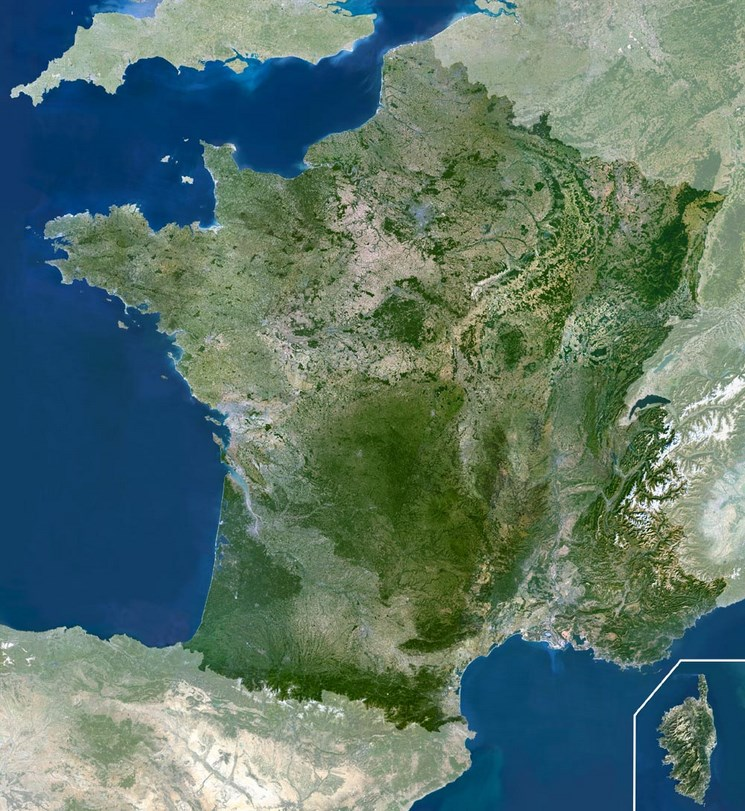
\includegraphics[scale=0.12]{figures/lib/france_satellite.jpg}};
    \node[align=center,below] at (photo.south) {Systeme modelise};
    % the local bounding box is to give a name to the pic:
    % http://tex.stackexchange.com/a/241737/32098
    \pic[local bounding box=carte] (carte) at (-5, 0) {france={scale 0.2}};
    \node[align=center,below] at (carte.south) {Modele};
    \draw[->] (carte) -- (photo.west) node[midway,above] {Represente} node[midway,below]{$\mu$};
\end{tikzpicture}


    \end{center}
    \caption{Relation entre système et modèle \protect\cite{favre2006ingenierie}}
    \label{fig:systemModele}
\end{figure}

Cette définition n'est pas restreinte à l'informatique et pourrait s'appliquer à 
n'importe quel système. 
La figure~\ref{fig:systemModele} reprend l'exemple connu de la cartographie où 
une carte géographique joue le rôle de modèle pour le territoire français qui joue le rôle su système réel.

L'intérêt de l'\gls{idm} est de produire des modèles exploitables informatiquement. 
Ceci n'est possible que si ces modèles sont décrits par des langages formels. Il 
devient alors important de bien définir ces langages à l'aide de métamodèles.

\subsection{Métamodèle et Conformité}
L'originalité de l'\gls{idm} ne réside pas dans la relation de représentation qui 
trouve plutôt son origine dans les méthodes de modélisation telles que Merise. L'apport de l'\gls{idm} est dans l'utilisation systématique de métamodèles pour la description des langages de modélisation. 

Il existe plusieurs définitions de la notion de métamodèle dans la littérature. 
Cependant la définition suivante est communément admise \cite{bezivin2004rapport}.
\\\

\begin{definition}
Un métamodèle est un modèle du langage de modélisation qui sert à exprimer les 
modèles.
\end{definition}

Une autre définition courante mais erronée de la notion de métamodèle suppose 
qu'un métamodèle est un modèle de modèle. La figure~\ref{fig:modelofmodel} 
reprend l'exemple de la cartographie évoquée plus haut. Nous appliquons 
récursivement la relation \textit{Représente} $(\mu)$ au territoire 
français. Ici une carte de la France joue le rôle de modèle du territoire 
français et un fichier XML joue le rôle de modèle de la carte. Dans ce contre 
exemple, le fichier XML n'est pas un métamodèle de la France. Un métamodèle 
n'est donc pas un modèle d'un modèle.

\begin{figure}[!ht]
    \begin{center}
        %\newsavebox\lstbox
%\begin{lrbox}{\lstbox}
%    \begin{minipage}{0.25\textwidth}
%        \begin{lstlisting}[style=xmlfig]
%<carte>
% <pays>France</pays>
% <regions>
%  <region>
%   <nom>Rhone-Alpes</nom>
%   <departement>
%    <nom>Drome</nom>
%   </departement>
%   ...
%  </region>
%  ...
% </regions>
%</carte>\end{lstlisting}
%    \end{minipage}
%\end{lrbox}

%\begin{tikzpicture}[]
%    \node (xml) at (-4, -1.86) {\usebox\lstbox};
%    \node[align=center,below] at (xml.south) {Modele};
%
%    % the local bounding box is to give a name to the pic:
%    % http://tex.stackexchange.com/a/241737/32098
%    \pic[local bounding box=carte] (carte) at (0, 0) {france={scale 0.2}};
%    \node[align=center,below] at (carte.south) {Modele};
%
%    \node[inner sep=4pt] (photo) at (7,-1.86) {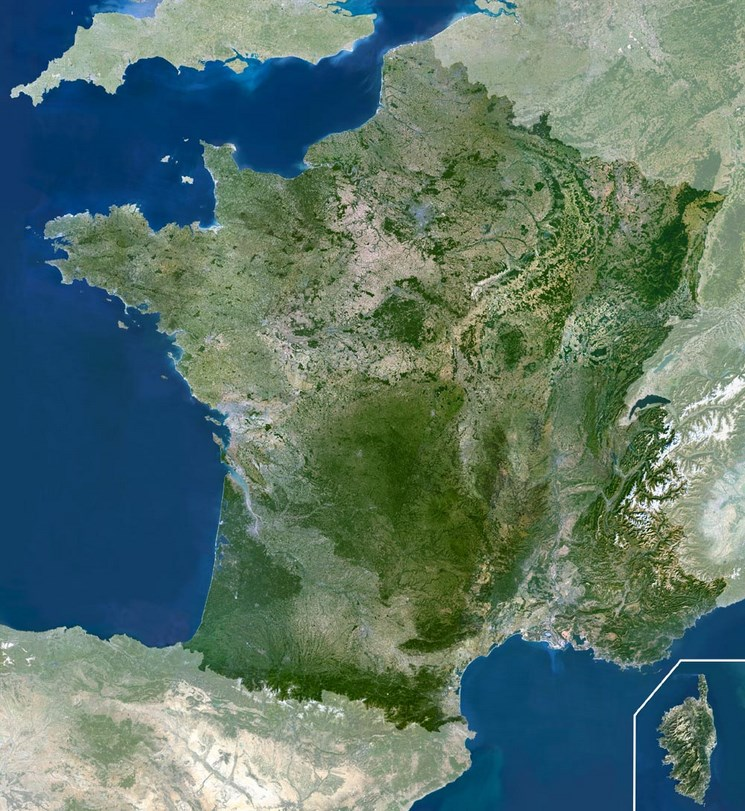
\includegraphics[scale=0.12]{figures/lib/france_satellite.jpg}};
%    \node[align=center,below] at (photo.south) {Systeme modelise};
%
%    \draw[->] (carte) -- (photo.west) node[midway,above] {Represente} node[midway,below]{$\mu$};
%    \draw[->] (xml) -- (carte.west) node[midway,above] {Represente} node[midway,below]{$\mu$};
%\end{tikzpicture}

\newsavebox\lstbox
\begin{lrbox}{\lstbox}
    \begin{minipage}{0.25\textwidth}
        \begin{lstlisting}[style=xmlfig]
<carte>
 <pays>France</pays>
 <region>
  <nom>Rhone-Alpes</nom>
  <departement>
   <nom>Drome</nom>
  </departement>
  ...
</carte>\end{lstlisting}
    \end{minipage}
\end{lrbox}
\begin{tikzpicture}[]
    \node (xml) at (-3.6, -1.4) {\usebox\lstbox};
    \node[align=center,below] at (xml.south) {Modele};

    % local bounding box to give a name to the pic: http://tex.stackexchange.com/a/241737/32098
    \pic[local bounding box=carte] (carte) at (0, 0) {france={scale 0.15}};
    \node[align=center,below] at (carte.south) {Modele};

    \node[inner sep=2pt] (photo) at (6,-1.4) {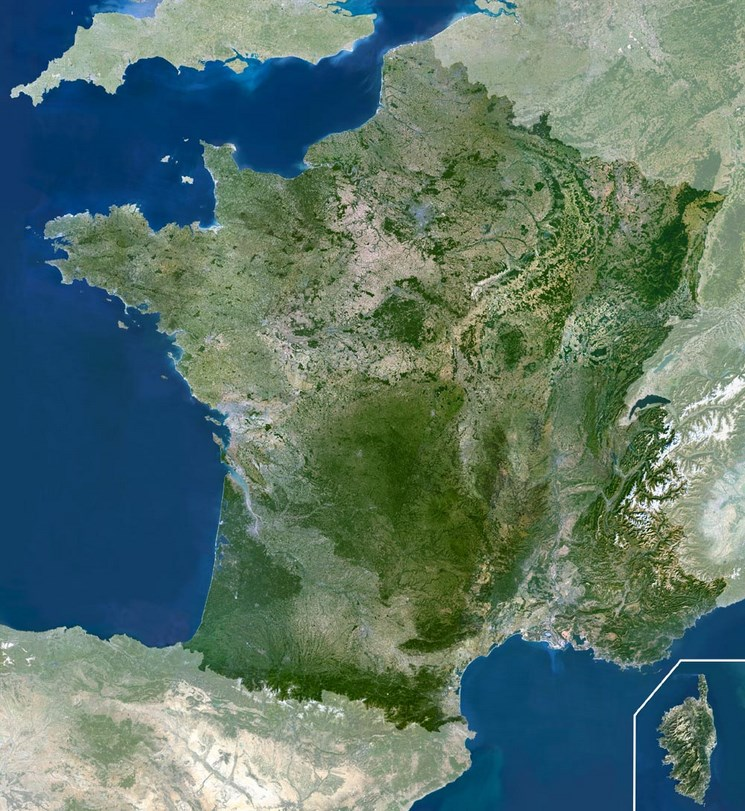
\includegraphics[scale=0.09]{figures/lib/france_satellite.jpg}};
    \node[align=center,below] at (photo.south) {Systeme modelise};

    % fleches
    \draw[->] (carte) -- (photo.west) node[midway,above] {Represente} node[midway,below]{$\mu$};
    \draw[->] (xml) -- (carte.west) node[midway,above] {Represente} node[midway,below]{$\mu$};
\end{tikzpicture}

    \end{center}
    \caption{Modèle de modèle selon l'exemple de la cartographie 
    \protect\cite{favre2006ingenierie}}
    \label{fig:modelofmodel}
\end{figure}

Par ailleurs, le concept de métamodèle induit la deuxième relation fondamentale 
de l'\gls{idm} liant un modèle à son métamodèle. Cette relation est nommée 
\textit{ConformeÀ} et notée $\chi$ \cite{bezivin2004search} 
\cite{favre2004towards}. La figure \ref{fig:carteFavre} reprend l'exemple de la 
cartographie où la légende de la carte joue le rôle de métamodèle pour 
une carte de la France. En effet, pour être lisible, la carte doit être conforme 
à la légende.

\begin{figure}[!htbp]
 \begin{center}
 % http://tex.stackexchange.com/a/7816/32098
\begin{tikzpicture}[
    title/.style={font=\scriptsize},
    textlgd/.style={font=\tiny,inner sep=1pt}]

    \pic[local bounding box=carte] (carte) at (0, 0) {france={scale 0.15}};
    \node[align=center,below] (modele) at (carte.south) {Modèle};

    \begin{scope}[scale=0.7,xshift=-130,yshift=-60]
        \draw (-1.7cm,-1.7cm) rectangle (1.6cm,2.5cm);
        % HACK: \clip does not accept options such as line width, but we want a
        % thin line so we make this the default for this scope. Since we also
        % want to keep the default line width for the dotted line, we copy its
        % value in a length as showed here:
        % http://tex.stackexchange.com/a/65811/32098
        \newlength{\defaultpgflinewidth}
        \setlength{\defaultpgflinewidth}{\pgflinewidth}
        \begin{scope}[ultra thin]
            \clip[draw] (0,0) circle (1cm);
            \draw[densely dotted,line width=\defaultpgflinewidth,step=.5cm,gray] (-1.4,-1.4) grid (1.4,1.4);
        \end{scope}
        \node[textlgd] (dpt) at (105:1.7cm) {Departements};
        \node[textlgd] (reg) at (-120:1.7cm) {Region};
        \draw[->] (reg) -- (-120:1cm);
        \draw[->] (dpt) -- (0.25,0.25);
        \draw[->] (dpt) -- (-0.25,0.25);
        \node (legende) [title] at (0,2.2cm) { Légende };
    \end{scope}
    \path (modele) -- +(-4.5,0) node[align=center] {Métamodèle};

    \node[inner sep=2pt] (photo) at (6,-1.4) {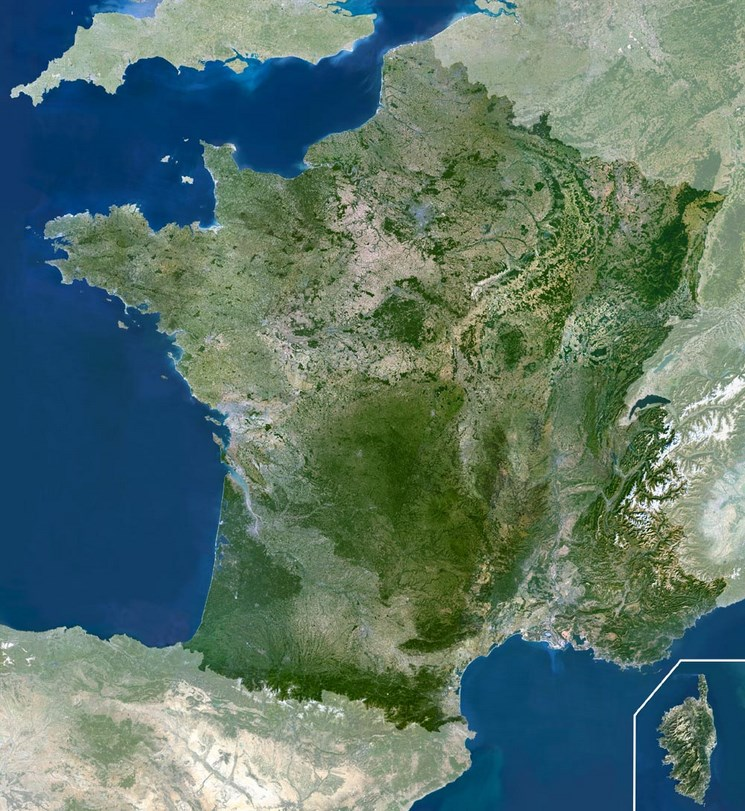
\includegraphics[scale=0.09]{figures/lib/france_satellite.jpg}};
    \path (modele) -- +(4.7,0) node[align=center] {Système modélisé};

   \draw[->] (carte) -- +(3.3,0) node[midway,above] {Représente} node[midway,below]{$\mu$};
   \draw[->] (carte) -- +(-3.2,0) node[midway,above] {ConformeÀ}  node[midway,below]{$\chi$};
\end{tikzpicture}

 \end{center}
 \caption{Relations entre système, modèles, métamodèle et langage de 
modélisation \protect\cite{favre2006ingenierie}}
 \label{fig:carteFavre}
\end{figure}

\section{Transformation de modèle}
Comme expliqué précédemment, la préoccupation majeure de l'\gls{idm} est de 
rendre les modèles opérationnels sur tout le cycle de vie des systèmes 
logiciels, depuis l'analyse et la conception jusqu'à la maintenance et 
l'évolution. La transformation de modèle se retrouve au cœur de l'\gls{idm} car 
c'est à travers elle que se fait l'automatisation des traitements apportés aux 
modèles. Dans cette section, nous donnons une définition de la 
transformation de modèle avant d'en présenter les types et les usages.

\subsection{Définition de la transformation de modèle}
L'\gls{omg} définit une transformation de modèle comme «~le processus consistant à 
convertir un modèle en un autre modèle d'un même système~» \cite{omg2011meta}. 

Kleppe et al. \cite{kleppe2003mda} proposent une définition moins générique en insistant sur l'aspect automatique de ce processus~:~«~une transformation de modèle 
consiste en la génération automatique d'un modèle source en un modèle cible, 
selon une description établie de cette transformation~». Cette définition 
implique qu'une transformation est décrite à un niveau 
d'abstraction au dessus de celui des modèles~:~au niveau d'un métamodèle auquel elle doit se conformer. 

Mens et Van Gorp \cite{mens2006taxonomy} étendent cette définition en considérant qu'une 
transformation est une opération qui peut avoir en entrée un ou plusieurs 
modèles source et en sortie un ou plusieurs modèles cible~: 

\begin{definition}
Une transformation génère automatiquement un ou plusieurs modèles cible à partir 
d'un ou plusieurs modèles source, selon une description établie de la 
transformation. 
\end{definition}

C'est cette dernière définition que nous adoptons dans ce document. Par 
ailleurs, notons que, si les métamodèles source et cible sont différents, la 
transformation est dite exogène. Si les métamodèles source et cible 
correspondent au même métamodèle, la transformation est dite endogène. Ces 
termes sont introduits par Mens et Van Gorp \cite{mens2006taxonomy}.

\subsection{Composants d'une transformation de modèle} 
La figure \ref{fig:composantTransfo} illustre les composants d'une 
transformation de modèle~:~les modèles source, les modèles cible, la définition 
de la transformation et le moteur qui va opérer la transformation selon sa 
définition. 

La description de la transformation définit la manière de transformer un ou plusieurs modèles source en un ou plusieurs modèles cible. Elle est créé dans 
un langage de transformation de modèle. Par exemple, si c'est un langage à base 
de règles, la description de la transformation consiste en un ensemble de règles 
de transformation à opérer sur les modèles cible \cite{kleppe2003mda}. 

Un moteur de transformation exécute ou interprète la description. Il applique 
donc la description aux modèles source pour produire les modèles cible en 
suivant les étapes ci-dessous \cite{tratt2005model}~:

\begin{itemize}
\item identifier l'élément du ou des modèles source à transformer~;
\item pour chaque élément identifié, produire l'élément cible qui lui est 
associé dans le ou les modèles cible~;
\item produire une trace de la transformation qui lie les éléments du ou des 
modèles cibles aux éléments du ou des modèles source.
\end{itemize}

\begin{figure}[!htbp]
 \begin{center}
   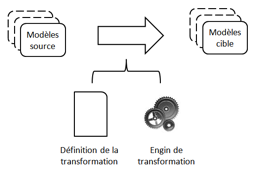
\includegraphics[width=0.7\textwidth]{figures/3_etat_de_l_art_IDM/composanttransfo.png}
 \end{center}
 \caption{Composants d'une transformation de modèle}
 \label{fig:composantTransfo}
\end{figure}

\subsection{Usages de la transformation de modèles }
Les transformations de modèles sont au cœur d'une démarche dirigée par les 
modèles~:~elles permettent d'automatiser les manipulations subies par les 
modèles telles que la modification, la création, l'adaptation, la composition ou 
encore le filtrage de modèles, à travers la réutilisation systématique 
d'informations contenues dans les modèles existants. 

Il est possible de recourir aux transformations de modèles sur tout le cycle de 
vie d'un système. Les usages les plus répondus sont le raffinement, 
l'intégration d'outils, la composition, l'analyse, la simulation et 
l'optimisation que nous présentons dans la suite de ce document. 


\subsubsection{Raffinement}

Le raffinement consiste à rajouter plus de détails au modèle initial. Ce type de 
transformation peut aussi bien être endogène (métamodèles source et cible 
identique) ou exogène (métamodèle source et cible différents). Le raffinement se 
prête parfaitement à toute la partie descendante du cycle en V où les modèles 
passent à des niveaux d'abstraction plus bas. Ceci revient à faire des 
transformations successives de type modèle-à-modèle et une transformation de 
type modèle-à-texte pour aboutir au code final.

Raffiner un modèle revient à décomposer des concepts de haut niveau, à choisir 
un algorithme particulier, à spécialiser un concept pour un contexte donné ou 
encore à le concrétiser sous forme d'une solution exécutable par une machine en 
générant le code à partir de modèles de plus haut niveau d'abstraction 
\cite{czarnecki2000intentional}. 

\subsubsection{Intégration d'outil}

Il existe une panoplie d'outils disponibles pour créer, manipuler, analyser ou 
encore simuler des modèles. Souvent ces outils utilisent des métamodèles 
internes et des espaces techniques qui leurs sont propres. Ainsi, l'échange de 
modèle entre ces outils est compromis et l'interopérabilité est fortement 
entravée. L'utilisateur se trouve obligé d'utiliser un seul et même outil sur 
tout le cycle de vie du système et ne peut donc pas tirer avantage des 
possibilités offertes par d'autres outils plus adaptés à ses besoins à certaines 
étapes.

L'intégration d'outil est une solution pour palier la divergence syntaxique et 
sémantique des outils et des langages de modélisation par le biais la 
transformation de modèle \cite{tratt2005model}. Ce type de transformation permet 
de naviguer entre deux métamodèles, de synchroniser des modèles qui évoluent 
séparément sur des outils distincts, de faire des mapping entre métamodèles pour 
maintenir la cohérence des modèles conformes à ces métamodèles. Il sera donc 
possible de faire appel à des outils mieux adaptés à chaque étape du cycle de 
vie.

\subsubsection{Composition}

Pour réduire la complexité inhérente à la modélisation et à l'analyse de grands 
systèmes, tels que les Smart Grids par exemple, il est possible d'adopter une 
approche par points de vue qui permet de séparer les préoccupations. Les modèles 
produits correspondent donc à ces différents points de vue qu'on peut ainsi 
valider séparément dans un premier temps. A l'issue de cette approche modulaire, 
on pourra composer ces modèles, c'est-à-dire les assembler, pour aboutir un 
modèle global du système.

Dans le cas le plus simple, les deux modèles à composer sont conformes à un même 
métamodèle. Cependant, il est aussi possible de composer deux modèles conformes 
à deux métamodèles différents. 

Les deux modèles à composer peuvent aussi présenter des concepts en commun. Deux 
techniques existent pour composer des modèles~:
%que nous illustrons dans la figure \ref{fig:compoExemple}~:

\begin{itemize}
\item la première technique consiste à les fusionner. Dans ce cas, le modèle 
final résultant de la composition doit contenir toutes les informations issues 
des modèles initiaux, sans duplication des informations communes 
\cite{bezivin2006canonical}.
\cite{fleurey2008generic} présente un framework générique capable de composer 
des modèles indépendamment de leurs langages de modélisation. L'approche 
consiste à identifier les éléments qui représentent le même concept dans les 
deux modèles à composer et à les fusionner dans un nouveau modèle qui représente 
une vue intégrée de ces concepts. Il est aussi possible de spécialiser le 
framework pour un métamodèle particulier mais qui reste conforme au \gls{mof}~;

\item la deuxième technique consiste à les tisser. Dans ce cas, on crée des 
correspondances entre les éléments qui représentent un même concept. Un 
métamodèle générique est créé pour définir les correspondances qui sont donc 
modélisées dans le modèle final. On y retrouve donc les éléments en commun 
dupliqués mais liés par un lien de correspondance. 
\end{itemize}

Il est à noter que le modèle issu du tissage de deux modèles $M_{A}$ et $M_{B}$ 
peut être utilisé comme modèle intermédiaire que l'on note $M_{T}$ pour la 
fusion de $M_{A}$ et $M_{B}$. Dans ce cas L'opération de fusion consiste à 
produire un modèle $M_{AB}$ en prenant comme entrée $M_{A}$, $M_{B}$ et $M_{T}$. 
Cette technique est notamment utilisée par \cite{del2007semi} pour la 
composition semi-automatique de modèles.

%\begin{figure}[!htbp]
% \begin{center}
%  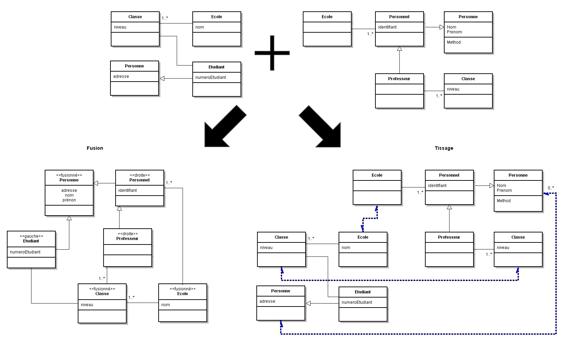
\includegraphics[width=1\textwidth]{figures/images/Chapitre1/compoExemple.png}
% \end{center}
% \caption{Exemple de composition de deux modèles}
% \label{fig:compoExemple}
%\end{figure}

\subsubsection{Simulation}

La transformation de modèle peut être utilisée pour simuler des modèles. En 
effet, une transformation de modèle peut mettre à jour le système modélisé. Dans 
ce cas, le modèle cible est une mise à jour du modèle source et la 
transformation est de type sur-place (modèles source et cible confondus). 

Par exemple, \cite{syriani2011multi} simule un comportement simple d'un jeu de 
Pacman en utilisant la transformation de modèle. La transformation spécifie les 
règles de transition qu'une instance du jeu peut prendre (Pacman et fantôme se 
trouvant dans la même case, Pacman et pomme se trouvant dans la même case, 
etc.). En ingénierie des langages, ceci revient à définir la sémantique 
opérationnelle d'un langage de modélisation. L'exécution de la transformation 
anime le modèle en fonction du comportement qu'on lui confère.

La transformation peut aussi être utilisée comme intermédiaire dans la 
simulation de modèle. Des modèles en entrée d'un outil de simulation externe 
sont produits par une transformation des modèles qu'on souhaite simuler. Cette 
technique permet de tirer profit d'outils de simulation existant sur le marché 
en utilisant l'intégration d'outils.

\subsubsection{Analyse et optimisation}

La transformation de modèle peut être utilisée pour les activités d'analyse de 
modèle. Une analyse simple telle que le calcul de métrique de similarité entre 
deux modèles via la transformation de modèle est donnée dans \cite{del2007semi} 
avec un modèle de transformation écrit en \gls{atl} \cite{jouault2006transforming}. 

Des analyses plus complexes sont possibles grâce à l'intégration d'outils 
d'analyse externes vers lesquels les modèles source sont transformés.

\cite{biehl2010integrating} propose d'utiliser la transformation de modèle pour 
l'analyse de sûreté de fonctionnement dans le domaine de l'automobile. Les 
modèles source sont transformés en modèles conformes au métamodèle de l'outil 
d'analyse de sûreté de fonctionnement retenu.
 
L'optimisation vise à améliorer les propriétés non fonctionnelles des modèles 
telle que l'évolutivité, la fiabilité, la modularité, etc. L'optimisation est 
typiquement utilisée sur les modèles d'architecture. Les transformations 
utilisées pour l'optimisation sont de types endogènes car on cherche à affiner 
la conception de modèles existants. La réingénierie est un exemple de 
transformation utilisée pour optimiser les modèles~:~on cherche à améliorer la 
maintenabilité, la lisibilité et l'évolutivité des modèles.


\subsection{Approches existantes pour la transformation de modèle}  
Le recours à la transformation de modèle est l'objet de recherches informatiques 
antérieures à l'apparition de l'approche \gls{idm}. Par exemple, les compilateurs 
utilisent la transformation pour passer du code source au fichier binaire 
\cite{aho1985compilers}. Ce type de transformation est restreint au domaine de 
la programmation informatique. La transformation de modèle embrasse un domaine 
plus large encore.

Nous trouvons dans la littérature plus d'une trentaine d'approches différentes 
de transformation de modèle \cite{syriani2011multi}. Czarnecki et Helsen 
proposent une classification de ces approches selon plusieurs critères tels que 
le paradigme retenu pour définir la transformation, la relation entre les 
modèles sources et cibles, la directivité de la transformation, le nombre de 
modèles cible et source, l'orchestration et l'ordonnancement des règles de 
transformation, etc. \cite{czarnecki2006feature}. \cite{blanc2011mda} définit les trois grandes catégories d'approches suivantes.

\begin{description}

\item[Par programmation]:~Les modèles offrent une interface qui permet d'écrire les transformations dans 
un langage de programmation. Mais cette technique relève plus de la 
programmation que de la modélisation. Ce sont en fait des applications 
informatiques qui ont la particularité de manipuler des modèles. L'avantage de 
cette approche est qu'elle utilise un langage de programmation généraliste tel 
que Java ou C++ pour écrire les transformations. Ainsi le programmeur n'a pas 
besoin d'apprendre un nouveau langage. Cependant ces applications ont tendance à 
devenir difficilement maintenables.

\item [Par template]:~Dans cette approche, des canevas des modèles cibles sont définis. Ces modèles contiennent des paramètres qui sont remplacés par les informations contenues 
dans les modèles source. Ce type de transformation est souvent utilisé pour les 
transformations qui génère des modèles dont la syntaxe concrète  est textuel.  Cette approche est associée au visitor-pattern qui va traverser la structure interne du modèle source. 
%Cette approche est utilisée par l'outil Enterprise Architect par exemple. 

\item [Par modélisation]:~Cette approche vise à appliquer les principes de l'\gls{idm} aux transformations de modèle elles-mêmes. Les modèles de transformation sont ainsi prennes, réutilisables et indépendants des plates-formes d'exécution  \cite{bezivin2006model}. Pour cela, des langages de modélisation dédiés à l'activité de transformation de modèles sont utilisés. Cette approche considère donc la transformation comme 
un modèle à part entière conforme à un métamodèle de transformation. La figure 
\ref{fig:TransfoPrincipe} illustre cette approche en positionnant la transformation par rapport aux niveaux d'abstraction de l'\gls{idm}. Elle corrobore 
ainsi la vision unificatrice de l'\gls{idm} à travers le paradigme du «~tout est 
modèle \cite{bezivin2005unification}.
\end{description}


\begin{figure}[!htbp]
 \begin{center}
  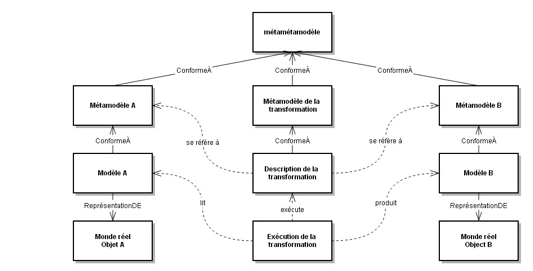
\includegraphics[width=1\textwidth]{figures/3_etat_de_l_art_IDM/transfoPrincipe.png}
 \end{center}
 \caption{Méta niveaux d'une transformation de modèle}
 \label{fig:TransfoPrincipe}
\end{figure}


\section{Langages et outils pour la transformation de modèle}
Sans viser à l'exhaustivité, nous introduisons succinctement quelques langages et outils 
dédiés à la transformation de modèles.  

\subsection{ATL}
\label{sec:ATL}
\gls{atl}\footnote{http://www.eclipse.org/atl/} est né de la volonté de proposer des langages de modélisation dédiés à la transformation de modèle en définissant un métamodèle 
et des outils pour l'exécution des transformations. 
%Il permet de réaliser des transformations de type modèle-à-modèle et de type modèle-à-texte.

\gls{atl} est un langage hybride (déclaratif et impératif) à base de contraintes \gls{ocl} \cite{jouault2006transforming}. 
%Une règle déclarative, appelée \textit{Matched rule}, permet de décrire 
%l'implémentation de mapping simples entre les modèles source et cible en 
%utilisant des patrons source (\textit{InPattern}) mappés avec les éléments 
%source et des patrons cibles (\textit{OutPattern}) mappés avec les éléments 
%cible. 

%L'approche impérative explicite les étapes d'exécution de la transformation à 
%travers les \textit{Helpers}. Le mécanisme de \textit{Helpers} permet en outre d'éviter la 
%redondance de code et la création de longues règles écrites en \gls{ocl}, ce qui 
%confère une meilleure lisibilité aux programmes \gls{atl}. 
%
%Une transformation écrite en \gls{atl} est composée d'un ensemble de règles qui 
%spécifient comment créer et initialiser les éléments des modèles cible. Il n'est 
%pas possible de spécifier l'ordre d'exécution des règles de transformation. Cet 
%ordre est établi automatiquement, sauf  pour les \textit{Lazy rules} 
%qui demandent de faire spécifiquement appel à elles. \gls{atl} est conforme au 
%méta-métamodèle \gls{mof} et est doté d'une syntaxe concrète textuelle. Il est intégré 
%à l'environnement Eclipse. Une transformation prend en entrée un ensemble de 
%modèles conformes au méta-métamodèle Ecore ou à KM3 \cite{jouault2006km3}.

%\gls{atl} ne prend pas en charge les transformations incrémentales. Il commence par 
%lire entièrement les modèles source et génère des modèles cible complet. Les 
%modifications manuelles dans les modèles cible ne sont donc pas préservées si 
%l'on opère une nouvelle transformation.

\gls{atl} peut réaliser des transformations sur place, c'est-à-dire, une 
transformation où le modèle source et le modèle cible sont confondus en 
utilisant le mode raffinement de modèle. 

%Cependant ce mode présente quelques limitations avec certaines fonctionnalités comme celle des \textit{Lazy rules}.

\subsection{QVT}
\gls{qvt} \cite{kurtev2008state} \cite{omg2011meta} est un standard de l'\gls{omg}. Le métamodèle de \gls{qvt} est conforme au \gls{mof}. Comme \gls{atl}, \gls{qvt} se base sur \gls{ocl} pour accéder aux éléments des modèles.
\gls{qvt} définit deux langages de transformation de type modèle-à-modèle. 
QVT \textit{Declarative} (QVTd)\footnote{http://projects.eclipse.org/projects/modeling.mmt.qvtd} est un langage déclaratif. QVT \textit{Operational} (QVTo) est un langage impératif\footnote{http://projects.eclipse.org/projects/modeling.mmt.qvt-oml}.

%QVT-R est un langage de transformation de haut niveau d'abstraction doté de 
%syntaxes concrètes textuelle et graphique. Les transformations, 
%bidirectionnelles, sont spécifiées sous forme de relations entre les modèles 
%source et cible. Une transformation a pour but de vérifier la cohérence entre 
%deux modèles, renforcer la cohérence en modifiant le modèle cible, synchroniser 
%deux modèles ou encore pour raffiner un modèle par une transformation sur-place. 
%La sémantique de QVT-R est définie par une transformation vers QVT-C.

%QVT-C est un langage de transformation de bas niveau qui sert de base pour 
%QVT-R. Les deux langages ont le même niveau d'expressivité. Une transformation consiste à définir un mapping entre les métamodèles source et cible en utilisant 
%des patterns. Contrairement à QVT-R, la traçabilité est explicitement définie à 
%travers les liens entre les métamodèles.
%
%QVT-OM est un langage de transformation impératif qui étend QVT-R avec des 
%constructions impératives basées sur une extension impérative de \gls{ocl}. Les 
%transformations sont unidirectionnelles mais établissent explicitement des 
%modèles de traçabilité.
%
%\gls{qvt} est aussi doté d'un mécanisme de \textit{graybox} qui permet de faire appel 
%à des algorithmes complexes écrits dans n'importe quel langage de programmation 
%et d'utiliser des librairies existantes. Mais ce mécanisme rend la transformation opaque puisqu'il n'est pas contrôlé par le moteur d'exécution. 
%Nous pouvons citer SmartQVT ou encore ModelMorf comme machines d'exécution de 
%transformation écrite en \gls{qvt}.

\subsection{Kermeta}
Kermeta\footnote{http://www.kermeta.org/} est un langage généraliste de méta-modélisation exécutable et de 
méta-programmation orientée objet qui peut aussi décrire des transformations de 
modèle. Intégré à EMF, il est doté d'un métamodèle conforme au \gls{mof} qu'il étend 
avec un langage d'action impératif utilisé pour écrire le corps des opérations 
définies sur les concepts d'une syntaxe abstraite (ce qui revient à doter une 
syntaxe abstraite d'une sémantique opérationnelle). On peut ainsi décrire 
n'importe quel traitement sur un modèle ce qui est assimilé à une transformation 
de modèle.

%Le langage d'action de Kermeta permet d'écrire des expressions impératives qui 
%spécifient explicitement la construction des éléments des modèles cible. A 
%l'inverse de QVT-OM, Kermeta n'est pas un langage à base de règles.  
%Kermeta est capable de gérer les exceptions mais les transformations 
%multidirectionnelles ne sont pas supportées par les outils d'exécution. Il en 
%est de même pour la transformation incrémentale.
%Les modèles source sont lus en une seule fois et les modèles cible sont produits complets lors de l'exécution de la transformation.

\subsection{Acceleo}
Acceleo\footnote{http://www.eclipse.org/acceleo/} est un langage de transformation de modèles pour lequel les modèles cible ont une syntaxe concrète textuelle. Il suit une approche de transformation par \textit{template}. Le template correspond au modèle cible qui prend la forme d'un texte avec des espaces réservés aux informations provenant des modèles source. Accelo utilise OCL pour accéder au modèles source.  

\section{L'Ingénierie Dirigée par les Modèles pour l'Architecture d'Entreprise}

L'\gls{idm} se cantonne souvent au processus de développement logiciel en offrant une aide supplémentaire à l'analyse et la validation des modèles de spécification et en automatisant certaines tâches à travers la génération de code par exemple. Mais des disciplines plus orientées métier telle que l'EA peuvent aussi tirer partie des avantages qu'apporte l'\gls{idm} à l'ingénierie logicielle. 

\subsection{Méta-modélisation en Architecture d'Entreprise}

Les cadres d'EA contribuent à réduire la complexité liée à un système telle que l'entreprise en décomposant celle-ci en plusieurs vues. Les architectes d'entreprise doivent ensuite représenter les artefacts qui composent ces différentes vue. Le recours aux techniques de modélisation n'est donc pas étranger à l'EA. Les architectes d'entreprise ont besoin d'une représentation claire et pertinente des composants de l'entreprise pour leur propre compréhension mais aussi pour faciliter la communication avec les autres parties prenantes comme les experts métier, les architectes fonctionnels, les architectes applicatifs, etc. 

Souvent, les cadres d'architecture ne préconisent pas de langages de modélisation en particulier et se contentent d'ériger un ensemble de bonnes pratiques. Pour représenter l'entreprise, les architectes utilisent alors leurs propres systèmes de notations. Si deux architectes appartenant à des filiales différentes d'une même entreprise utilisent des notations différentes, des problèmes de communication, de collaboration et d'interopérabilité à l'échelle de l'entreprise risquent d'apparaître. L'architecture de l'entreprise perd alors de sa crédibilité en tant que référentiel d'entreprise.

Graphiques ou textuelles, ces notations manquent de plus d'une sémantique précise et formalisée entrainant la création de modèles purement contemplatifs. Les outils de visualisation et d'analyse sont d'autant plus difficiles à développer.

L'\textit{Open Group} propose de mettre en cohérence les notations utilisées en EA en créant un langage de modélisation standardisé nommé Archimate. Archimate sert ainsi à décrire l'entreprise, sa structure organisationnelle, ses processus, ses règles métier ou encore son SI. Archimate est un langage de représentation graphique utilisé pour documenter et à communier les architectures d'entreprise au sein d'une même organisation ou entre différentes organisations. Archimate est en outre étroitement lié au cadre d'architecture TOGAF. 

Bien que concis, le métamodèle d'Archimate vise à couvrir la majorité des concepts intervenants dans la création d'une architecture d'entreprise. Archimate utilise trois vues~:~métier, applicative et technique. Pour chacune des vues, trois types d'éléments différents sont spécifiés~:~structure active, comportement et structure passive (voir figure \ref{fig:archimate}). Les structures actives correspondent aux éléments dotés d'un comportement. Il peut s'agir d'un acteur métier, d'un module applicatif ou d'un élément de l'infrastructure technique. Le comportement est défini comme un ensemble d'activités ou de tâches poursuivies par un ou plusieurs éléments de la structure active. Il peut s'agit par exemple d'un processus métier. La structure passive comportent les éléments manipulés par les éléments de la structure active, comme par exemple les objets métier. 

\begin{table}[!ht]
    \vspace*{0.5em}
    \begin{center}
        \setlength{\mytablewidth}{\textwidth}
\setlength{\myfirstcolwidth}{\dimexpr0.23\mytablewidth-2\tabcolsep\relax}
\setlength{\mycolwidth}{\dimexpr0.26\mytablewidth-2\tabcolsep\relax}

\begin{tabulary}{\mytablewidth}{m{\myfirstcolwidth}m{\mycolwidth}m{\mycolwidth}m{\mycolwidth}}
    % \cmidrule[\heavyrulewidth]{2-4}
    & \centbf{Structure passive} & \centbf{Comportement} & \centbf{Structure active}\
    \tabularnewline\cmidrule{2-4}
    \hfill \textbf{Métier} & \tikzmark{tabletop} & & \
    \tabularnewline\cmidrule{2-4}
    \hfill \textbf{Application} & & & \
    \tabularnewline\cmidrule{2-4}
    \hfill \textbf{Techonologie} & \tikzmark{tablebottom} & & \
    \tabularnewline\cmidrule{2-4}
\end{tabulary}

\begin{tikzpicture}[overlay,remember picture]
    \def\mytablecolwidth{3.291}  % ~ column width (found manually)
    \def\mytableleftof{-0.21}  % ~ first column offset (found manually)
    \newcommand\drawcolsep[2]{%
    \draw[#2] let \p3=(tabletop), \p4=(tablebottom) in ($(\x3,\y3)+(\mytableleftof+#1*\mytablecolwidth,0.45)$) -- ($(\x3,\y4)+(\mytableleftof+#1*\mytablecolwidth,-0.22)$);}
    \drawcolsep{0}{}
    \drawcolsep{1}{dotted}
    \drawcolsep{2}{dotted}
    \drawcolsep{3}{}
\end{tikzpicture}

    \end{center}
 \caption{Composants du langage Archimate}
 \label{fig:archimate}
\end{table}

Le métamodèle du langage Archimate est un adossé d'une syntaxe concrète graphique permettant visualiser les modèles. Il associe par exemple des couleurs différentes aux éléments en fonction de leur type. Les éléments de type structure active sont bleus, ceux de type comportement sont jaunes et enfin ceux de type structure passive sont verts. Mais aucune sémantique standard d'exécution n'est formalisée. Les modèles d'architecture sont ainsi souvent purement contemplatifs et les outils implémentant Archimate n'offrent pas la possibilité d'exécuter ces modèles à des fins d'analyse de structure et de comportement. 

\subsection{Approches d'Architecture d'Entreprise recourant à l'Ingénierie Dirigée par les Modèles}

L'\gls{idm} a prouvé sa capacité à adresser des systèmes complexes \cite{france2007model}. L'application des techniques de l'\gls{idm} aux approches d'EA font l'objet de quelques rares travaux \cite{bruneliere2013support}. Les travaux de \cite{frankel2003zachman} font figure de précurseurs. Ces derniers décrivent un mapping entre le cadre Zachman et les vues \gls{mda} (figure \ref{fig:mapping-zachman-mda}). Mais le périmètre de ces travaux se réduit à l'architecture IT de l'entreprise plutôt qu'à l'entreprise dans son ensemble.

\begin{table}[!ht]
    \vspace*{0.5em}
    % Resources:
% Arrows: http://tex.stackexchange.com/a/60627/32098
% Rotating tikz label: http://tex.stackexchange.com/a/115565/32098

\setlength{\mytablewidth}{\textwidth}
\setlength{\myfirstcolwidth}{\dimexpr0.19\mytablewidth-2\tabcolsep\relax}
\setlength{\mycolwidth}{\dimexpr0.18\mytablewidth-2\tabcolsep\relax}
\setlength{\mylastcolwidth}{\dimexpr0.05\mytablewidth-2\tabcolsep\relax}
\newcolumntype{C}[1]{>{\centering\arraybackslash}m{#1}}
\newcommand\mycell[1]{{\tiny{#1}}}

\begin{adjustbox}{width=\mytablewidth,center}
    \scriptsize
    \begin{tabulary}{\mytablewidth}{m{\myfirstcolwidth}C{\mycolwidth}C{\mycolwidth}C{\mycolwidth}C{\mycolwidth}C{\mycolwidth}m{\mylastcolwidth}}
        % \cmidrule[\heavyrulewidth]{2-6}
        \mrows{2}{}\tikzmark{zachmantopleft} \
        & \centbf{Données} \
        & \centbf{Fonctions} \
        & \centbf{Personnel} \
        & \centbf{Temps} \
        & \centbf{Motivation}\tikzmark{zachmantopright} \
        & \
        \tabularnewline
        & \centit{Quoi} \
        & \centit{Comment} \
        & \centit{Qui} \
        & \centit{Quand} \
        & \centit{Pourquoi} \
        & \
        \tabularnewline\cmidrule[\lightrulewidth]{1-6}

        \tikzmark{zachmanlefttop}\textbf{Exécutif}
        & {\tiny{Identification}} \
        & {\tiny{Identification}} \
        & {\tiny{Identification}} \
        & {\tiny{Identification}} \
        & {\tiny{Identification}} \
        & \
        \tabularnewline
        \textit{Planification} \
        & {\tiny{des données}} \
        & {\tiny{des processus}} \
        & {\tiny{des responsabilités}} \
        & {\tiny{des échéances}} \
        & {\tiny{des motivations}} \
        & \multibrace{4}{\mycolwidth}{\gls{cim}} \
        \tabularnewline\cmidrule[\lightrulewidth]{1-6}

        \textbf{Management}\newline\textit{Définition} \
        & {\tiny{Définition des données}} \
        & {\tiny{Définition des processus}} \
        & {\tiny{Définition des responsabilités}} \
        & {\tiny{Définition des échéances}} \
        & {\tiny{Définition des motivations}} \
        & \
        \tabularnewline\cmidrule[\lightrulewidth]{1-6}

        \textbf{Architecte}\newline\textit{Conception}  \
        & {\tiny{Conception des données}} \
        & {\tiny{Conception des processus}} \
        & {\tiny{Conception des responsabilités}} \
        & {\tiny{Conception des échéances}} \
        & {\tiny{Conception des motivations}} \
        & \multibrace{2}{\mycolwidth}{\gls{pim}} \
        \tabularnewline\cmidrule[\lightrulewidth]{1-6}

        \textbf{Ingénieur}\newline\textit{Spécification} \
        & {\tiny{Spécification des données}} \
        & {\tiny{Spécification des processus}} \
        & {\tiny{Spécification des responsabilités}} \
        & {\tiny{Spécification des échéances}} \
        & {\tiny{Spécification des motivations}} \
        & \multibrace{2}{\mycolwidth}{\gls{psm}} \
        \tabularnewline\cmidrule[\lightrulewidth]{1-6}

        \tikzmark{zachmanleftbottom}\textbf{Technicien}\newline\textit{Implémentation} \
        & {\tiny{Implémentation\newline des données}} \
        & {\tiny{Implémentation\newline des processus}} \
        & {\tiny{Implémentation\newline des responsabilités}} \
        & {\tiny{Implémentation\newline des échéances}} \
        & {\tiny{Implémentation\newline des motivations}} \
        & \multibrace{2}{\mycolwidth}{Code} \
        \tabularnewline\cmidrule[\heavyrulewidth]{1-6}
    \end{tabulary}
    \begin{tikzpicture}[overlay,remember picture]

        % top horizontal arrow
        \draw[<->] let \p1=(zachmantopleft), \p2=(zachmantopright) in ($(\x1,\y1)+(1.5,0.4)$) -- node[label=Abstractions (colonnes)] {} ($(\x2,\y2)+(0,0.4)$);

        % left vertical arrow
        \draw[<->] let \p3=(zachmanlefttop), \p4=(zachmanleftbottom) in ($(\x3,\y3)+(-0.3,0.3)$) -- node[label={[label distance=-2ex, text depth=3ex, label position=above, rotate=90]above:Perspectives (lignes)}] {} ($(\x3,\y4)+(-0.3,-0.5)$);
    \end{tikzpicture}
\end{adjustbox}

    \caption{Mapping Zachman/\gls{mda} \protect\cite{frankel2003zachman}}
    \label{fig:mapping-zachman-mda}
\end{table}

\cite{clark_towards_2014} proposent d'étendre la démarche \gls{mda},  traditionnellement appliquée au développement de systèmes informatiques, à l'ensemble de l'entreprise pour mettre en place une organisation dirigée par les modèles ou MDO (\textit{Model Driven Organisation}). Comme l'illustre la figure \ref{fig:mdo}, une MDO comprend un modèle de l'organisation (\textit{Model of the Organization}), un modèle spécifique à une plateforme (\textit{Platform Specific Model}) et une plateforme d'entreprise (\textit{Platform for Organization}). 

\begin{figure}[!htbp]
 \begin{center}
   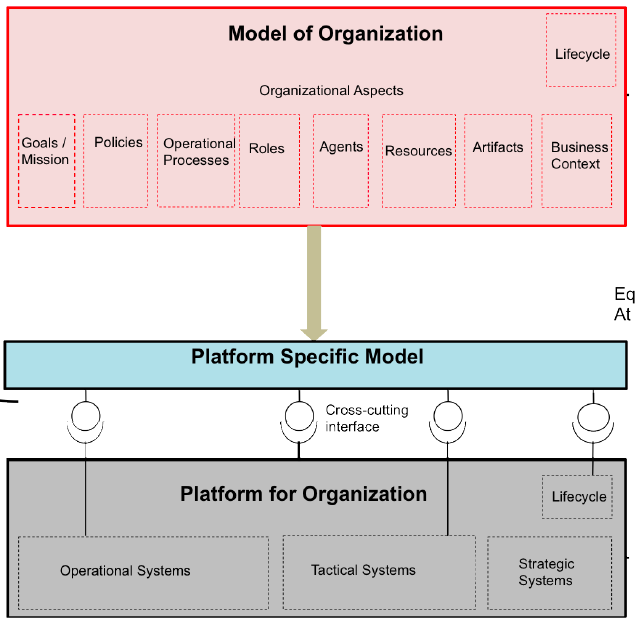
\includegraphics[width=0.7\textwidth]{figures/3_etat_de_l_art_IDM/mdo.png}
 \end{center}
 \caption{Architecture d'une organisation dirigée par les modèles (à remplacer par une belle figure) \protect\cite{clark_towards_2014}}
 \label{fig:mdo}
\end{figure}

Le modèle de l'organisation correspond à l'ensemble des modèles métier présentant les processus, les objectifs, les acteurs, les ressources. L'organisation fait appel à son IT pour réaliser ses objectifs métier. L'ensemble du système informatique correspond alors à la plateforme opérationnelle de l'entreprise. Comme pour \gls{mda}, le modèle spécifique à une plateforme est dérivé du modèle de l'organisation et sert de pivot pour générer automatiquement la plateforme de l'organisation par transformation de modèles.

Dans leurs travaux, \cite{clark_towards_2014} proposent un cadre théorique et une étude d'opportunité quant à la généralisation de \gls{mda} à l'échelle de l'entreprise. Cependant \gls{mda} reflète la vision particulière de l'\gls{omg} concernant l'\gls{idm}. L'approche \gls{mda} est de ce fait restreinte aux standards de l'\gls{omg}. Les travaux de Clark et al. sont donc limités par l'approche \gls{mda} (celle-ci étant un sous-ensemble de l'\gls{idm}).

L'\gls{idm} préconise le recours aux modèles exécutables pendant tout le cycle de vie du système à implémenter. Cependant, à l'échelle d'une entreprise, l'utilisation de ce type de modèles est souvent limité à l'implémentation des systèmes informatiques, c'est à dire à l'implémentation de la vue applicative et la vue technique d'une architecture d'entreprise. L'usage des modèles en tant artefacts exécutables est peu commun en EA \cite{kulkarni_modelling_2013}.

Parmi les travaux mettant à contribution les techniques de l'\gls{idm} nous citons ceux de \cite{clark2011leap}. Ces derniers proposent un langage concis et exécutable pour modéliser et simuler les différentes vues d'une architecture d'entreprise. Cependant ce langage est principalement textuel. Il offre une visualisation graphique des aspects structuraux d'une organisation sous la forme d'un diagramme de classes. Mais la syntaxe concrète pour la spécification du comportement est essentiellement textuelle. L'adoption de ce langage par les parties prenantes à profil non technique n'est pas évidente. Or l'EA a pour vocation d'offrir un référentiel compréhensible et partagé par toutes les parties prenantes.

Les travaux de \cite{bruneliere2013mde} tirent profit des capacités de l'\gls{idm} à automatiser la manipulation des modèles pour offrir une assistance dans la création et la visualisation d'architectures d'entreprise. La plateforme proposée s'appuie sur \gls{togaf} et fournit un support pour la gouvernance et la prise de décision souvent gérées manuellement. Ces travaux se focalisent sur les techniques \gls{idm} permettent de (1) concevoir une cartographie de l'existant par rétro ingénierie à partir des données disponibles dans le SI, (2) adapter la représentation graphique des modèles au besoin des utilisateurs concernés, (3) gérer plusieurs vues d'un même système et automatiser leur manipulation. \cite{bruneliere2013mde} démontrent que les techniques de l'\gls{idm} apportent des réponses à certaines limitations liées aux pratiques actuelles d'EA mais ne supportent pas la simulation des modèles obtenus. 

\cite{manzur2015xarchimate} utilisent les techniques de l'\gls{idm} (en particulier la métamodélisation) pour analyser la composante dynamique des modèles Archimate à travers la simulation de propriétés non fonctionnelles. Dans un premier temps, ils réduisent le métamodèle  d'Archimate en ne retenant que les concepts indispensables à la modélisation des propriétés non fonctionnelles. Comme Archimate est d'abord conçu pour modéliser la structure des architectures d'entreprise, \cite{manzur2015xarchimate} enrichissent dans un deuxième temps le métamodèle obtenu avec deux autres types de concepts (1) des concepts pour décrire le comportement et (2) des concepts uniquement liés à l'exécution. 

Les travaux de \cite{manzur2015xarchimate} illustrent les avantages de la métamodélisation et la définition d'une sémantique formelle pour l'exécution de modèles d'architecture d'entreprise. Néanmoins, ces travaux ne concernent que les propriétés non fonctionnelles des modèles d'architecture. Ces travaux formalisent aussi bien le métamodèle de la vue métier  que ceux des vues applicative et technique. Cependant la simulation des différentes se fait séparément les unes des autres. L'approche ne permet donc pas de simuler simultanément l'ensemble de l'architecture. 


%{\color{gray}
%
%Approches et leurs limites
%
%Mapping Zachman/\gls{mda} X
%
%Manzul X
%
%Jordi Cabot X
%
%Model Driven Organisation X
%
%LEAP X
%
%Thales reconfiguration  : Les modèles exécutables et leurs bénéfices}



\subsection{Langages exécutables pour l'Architecture d'Entreprise}

L'automatisation de l'analyse des modèles d'architecture d'entreprise s'avère particulièrement cruciale dans le contexte particulier des Smart Grids~:~évolution des cadres législatifs,  apparition de nouveaux partenaires, hétérogénéité des interactions avec les clients finaux via les compteurs intelligents, les smartphones, les tablettes tactiles, etc. Or l'exécution des modèles est indispensable à l'automatisation de l'analyse de leur structure et de leur comportement. Exécuter des modèles apporte ainsi une aide précieuse à la validation d'une architecture d'entreprise dès les premières phases de son cycle de vie et augmente son agilité et son évolutivité. D'une part, l'exécution des modèles facilite leur exploration  par les experts métier en levant les ambiguïtés engendrées par les modèles purement contemplatifs. D'autre part, exécuter des modèles permet d'évaluer et de comparer des architectures de manière objective en définissant des métriques et des indicateurs d'évaluation. 

L'exécution des modèles est rendue possible par la définition d'une sémantique exécutoire du langage dans lequel ces modèles sont exprimés. La sémantique d'un langage correspond au sens que peuvent prendre les concepts manipulés et leurs agencements lorsqu'ils sont instanciés au niveau des modèles \cite{jezequel2012ingenierie}. La définition de la sémantique du langage dépend de l'objectif poursuivi : simulation, génération de code, vérification, compilation, etc. L'expression de la sémantique d'un langage fait l'objet d'intenses recherches en ingénierie des langages, et en particulier sous la thématique des langages formels \cite{kleppe2007language}. 

Comme l'atteste le manifeste d'IBM \cite{chesbrough2006research}, les axes principaux de l'\gls{idm} sont (1)~les standards ouverts, (2)~l'automatisation et (3)~la représentation directe. Compte tenu de ces axes, pour modéliser les différentes vues d'une architecture d'entreprise, nous préconisons l'utilisation de \textbf{langages standardisés, exécutables et compréhensibles} par les acteurs concernés par la modélisation d'architectures d'entreprise pour les Smart Grids. 

Nous identifions plusieurs langages, issus de l'ingénierie des langages et en particulier de l'IDM, pouvant satisfaire ces critères~:

\begin{itemize}

\item Un sous-ensemble de UML\footnote{http://www.omg.org/spec/UML/} limité au diagramme de classes et au diagramme d'activité possède désormais une sémantique d'exécution décrite par le standard fUML\footnote{http://www.omg.org/spec/FUML/} (\textit{Foundational UML}). Les diagrammes de classes conviennent pour la description des modèles d'information tandis que les diagrammes d'activité sont adaptés à la description de la dynamique d'un modèle et au comportement attendu des fonctions~;

\item Le standard BPMN\footnote{http://www.omg.org/spec/BPMN/2.0/} (\textit{Business Process Model and Notation}) est un langage de modélisation graphique permettant de décrire tous les aspects d'un processus métier à l'aide d'un seul type de diagramme. Ce formalisme présente l'avantage d'avoir une sémantique d'exécution bien définie permettant le développement d'outils pour la simulation de modèles de processus métier. BPMN est parfaitement adapté à la description de processus métier~;

\item Le standard \gls{ocl}\footnote{http://www.omg.org/spec/OCL/} est un langage textuel standard d'expression de contraintes. Il est adosser à UML pour exprimer les propriétés difficiles à capturer dans des diagrammes UML. L'exécution d'\gls{ocl} se fait à travers la transformation de modèle en ciblant un langage d'expression de contrainte de plus bas niveau qui soit exécutable comme MiniZinc \cite{nethercote2007minizinc}, ou à travers son utilisation au niveau du métamodèle avec OCLinEcore\footnote{wiki.eclipse.org/OCL/OCLinEcore}.

\end{itemize}











    \part{Contribution}
	\chapter{Limites des pratiques d'Architecture d'Entreprise actuelles et 
proposition}
\label{ch:demarche}

\PartialToc

Créer des modèles d'architecture d'entreprise à des fins d'analyse par 
simulation implique de suivre un processus précis. L'objectif de notre travaux 
est de définir le processus de modélisation et de simulation à adopter, les 
rôles impliqués, les artefacts conceptuels requis, ainsi que les outils et les 
langages adéquats pour mener des analyses de structure et de comportement. 

Notre contribution est double. Tout d'abord, nous proposons une démarche de 
modélisation et d'analyse qui s'appuie sur un cadre d'architecture multi-vues. 
Nous dotons ce cadre d'architecture d'une vue supplémentaire qui est est la vue 
intégration. Cette vue a pour but d'adresser les problématiques de cohérence et 
d'alignement. Ensuite, nous mettons à profit les langages et standards de l'IDM 
permettant de modéliser et de simuler les architectures d'entreprise. 


%In this section, we present our approach and we apply it on the case study of 
%managing an electric vehicles fleet. Our contribution is twofold. First, we 
%propose a multi-view framework for EA with an additional view: the integration 
%view. This view aims to address consistency and alignment issues. Second, we 
%use 
%executable and standardized languages from MDE to model and simulate EA.

\section{Analyse des pratiques courantes d'Architecture d'Entreprise}

	\subsection{L'Architecture d'Entreprise pour la documentation et la 
communication}
	L'EA permet de capturer les composants de l'entreprise dans leurs états 
courants et désirés. La manière employée la plus courante de représenter ces 
composants reste la documentation \cite{barn2013enterprise}. Ces documents 
couvrent des aspects tels que les processus métier, les fonctions, les 
applications et l'infrastructure technique de l'entreprise, ainsi que leurs 
relations. Pour remplir leur rôle de référentiel d'entreprise, ces documents 
doivent être précis et régulièrement mis à jour. L'activité de documentation en 
EA telle que pratiquée actuellement est confrontés à des obstacles majeurs 
empêchant la production des documents pertinents et tenant lieu de feuille sur 
toute la trajectoire de l'entreprise~: de son état actuel à son état désiré.
	
	Pour commencer, la complexité de l'entreprise se retrouve dans sa 
représentation. En 
effet, une entreprise comme \gls{erdf} comporte des milliers de processus métier 
et des milliers d'applications supportant ses activités. Ces processus et ces 
applications sont de plus fortement interdépendants. Par conséquent, l'effort à 
fournir pour produire une documentation d'architecture pertinente est 
considérable. De plus, maintenir ces documents à jour n'est pas aisé du fait (1) 
du grand nombre d'artefacts à gérer et (2) du manque d'outils adéquats comme le 
confirment Shah et al. \cite{shah2007frameworks} et Roth et al. 
\cite{roth2013enterprise}. Or si la documentation n'est pas convenablement mise 
à jour, la valeur ajoutée et la crédibilité de l'EA sont remises en doute par 
l'ensemble de l'entreprise. 
	
	En outre, l'EA nécessite de collecter des informations provenant d'unités et de 
services différents (autant stratégique, opérationnelle ou support). Cette 
collecte est bien souvent centralisées au niveau du entité IT de l'entreprise, 
où une seule équipe est chargée d'acquérir les informations provenant des autres 
entités. Cette étiquette IT fait souvent préjudice aux efforts d'EA au sein de 
l'entreprise en la réduisant à de l'architecture IT. Zachman déplore cet état de 
fait, soulignant qu'il est nécessaire que l'EA transcende la sphère de l'IT et 
désignant l'EA comme «~l'enjeu du siècle~» \cite{zachman1997enterprise}.
 %-> team organization 
	
	De plus, les documents d'EA ne sont pas homogènes. Selon leurs besoins, les 
membres de l'équipe responsable de la documentation ont en effet tendance à 
utiliser des représentations hétérogènes. Shah et al. \cite{shah2007frameworks} 
font le constat que les équipes d'EA utilisent de surcroît plusieurs outils 
différents pour produire ces représentations aboutissant à une documentation 
ambigüe. Expliciter et exprimer les relations entre les représentations n'en est 
que laborieux et malaisé et la cohérence de l'ensemble de l'architecture s'en 
trouve ainsi compromise.
	
	Pour finir, la valeur ajoutée de l'EA diminue si la documentation produite 
n'est pas 
régulièrement mise à jour. Comme expliqué dans la section , les documents d'EA 
correspondent la plupart du temps à des modèles purement contemplatifs. C'est à 
notre avis, l'une des raisons qui expliquent le manque certain d'outils 
permettant d'automatiser cette mise à jour, voire même d'automatiser l'analyse 
de l'architecture d'entreprise comme expliqué dans la section suivante.
	

	\subsection{L'Architecture d'Entreprise pour l'analyse}
	
	L'analyse des composants métier, fonctionnel, applicatif et technique de 
l'entreprise est limitée par la manière dont ces composants sont représentés, 
c'est à dire sous la forme de documentation. Comme ce type de représentation ne 
permet pas l'automatisation de l'analyse, dans la pratique, les choix 
d'architecture repose entièrement sur le bon sens, à l'expérience et à 
l'expertise de l'architecte d'entreprise. Comme pour la documentation, l'analyse 
de l'architecture d'une grande entreprise est une activité éprouvante et 
chronophage à cause du grand nombre d'artefacts manipulés et de leurs forte 
interdépendance. Les praticiens mènent souvent les activités d'analyse 
manuellement \cite{barn2013enterprise}, sans le support d'outils intégrant 
naturellement les cadres d'architecture.
	
	D'une part, l'analyse de la structure et du comportement de entreprise permet 
d'acquérir une connaissance plus approfondie de l'ensemble de l'architecture. La 
documentation de l'architecture telle que décrit dans la section précédente est 
souvent sources d'erreurs à étant donnée la grande quantité et la forte 
interdépendance des artefacts manipulés \cite{kaisler_enterprise_2005}. Analyser 
cette documentation est d'abord indispensable à la détection de ces erreurs de 
représentation.
	
	Ensuite, Notre tour d'horizon des pratiques actuelles nous mène à constater que 
l'EA joue un rôle prépondérant durant les phases de description de l'existant et 
de spécification du système à mettre en œuvre mais qu'elle n'est pas exploitée 
dans toute sa potentialité. L'entreprise gagnerait à promouvoir l'architecture 
d'entreprise au rang de référentiel accompagnant l'entreprise sur toute sa 
trajectoire (de la spécification à la conception), et en particulier pour 
anticiper les incohérences potentielles entre les besoins formulés par le métier 
et leurs implémentations finales au niveau du SI.
	
	Pour ces travaux de recherches, plusieurs cas d'études ont été examinés, dont 
notamment la régulation de tension sur le réseau électrique 
\cite{seghiri2014simulation}, le pilotage d'une batterie chez un particulier 
\cite{seghiri2012animation} et la gestion d'une flotte de véhicules électriques 
\cite{seghiri2015simulation}. Qu'il s'agisse d'un projet de recherche européen 
(le pilotage d'une batterie chez un particulier), d'un projet interne à EDF (la 
régulation de tension), ou d'un projet opérationnel impliquant EDF ainsi que 
d'autres partenaires (la gestion d'une flotte de véhicules électriques), la 
documentation relative à l'architecture ne va pas au delà de la description 
générale des fonctionnalités attendues et ne permet pas d'analyser afin de les 
valider la structure et le comportement du système avant son implémentation 
finale. Pour accéder à un niveau de détails suffisant à analyser l'architecture 
du système avant son implémentation, une rétro-ingénierie du système final et 
des échanges avec les développeurs et les concepteurs ont été nécessaires. Ces 
constatations tirées du terrain rejoignent donc les conclusions de l'état de 
l'art concernant les limites des « modèles contemplatifs ».
	
	D'autre part, les mises en œuvre courantes d'EA adoptent une approche 
descendante où l'architecte d'entreprise ne fait qu'aligner le SI à la stratégie 
de l'entreprise en considérant cette dernière comme acquise. Une démarche 
descendante implique que la vision et les grandes lignes de la stratégie sont 
conçues en amont de l'EA et indépendamment de la réalité du SI qui va 
l'implémenter. Les choix stratégiques sont alors faits dans « une tour d'ivoire 
» et sont ainsi déconnectés de la réalité du SI. Il nous paraît au contraire 
important que l'analyse de l'architecture d'entreprise permettre d'évaluer et 
d'éclairer les choix stratégiques eux-mêmes, en plus de planifier leur 
déclinaison au niveau du SI. 
	
	Cette vision rejoint celle de l'école de pensée « Enterprise System 
Architecting » décrite par Lapalme \cite{lapalme2012three} et présentée dans la 
section~\ref{Lapalme}. Cependant, les approches d'analyse telles que pratiquées 
actuellement ne permettent pas d'y parvenir. L'analyse et la validation de la 
stratégie est désincarnée de l'EA. Par exemple, les algorithmes d'optimisation 
et de simulation de processus métier s'adressent uniquement aux analystes métier 
et ne sont pas couplés à la cartographie du patrimoine applicatif et aux 
capacités de l'infrastructure technique. Inversement, l'analyse de 
l'architecture d'entreprise se cantonne à valider la robustesse et la résilience 
du SI en dressant l'inventaire des applications d'entreprise, des interfaces 
logiciels, les serveurs d'application et leur aptitude à mettre en œuvre la 
stratégie de l'entreprise, sans jamais remettre celle-ci en question. 
	
	Appliquée à l'EA, l'approche descendante consiste décomposer les éléments d'une 
vue supérieure en éléments plus détaillés dans la vue inférieure, présumant que 
la recomposition des éléments de la vue inférieure correspondra parfaitement aux 
éléments de la vue supérieure. Or, des travaux de recherche portant sur la 
complexité des SI actuels soulignent que des propriétés « émergentes » 
apparaissent quand un grand nombre de systèmes complexes sont fortement 
interconnectés \cite{bullock2004complexity}, comme c'est que cas de l'IT d'une 
entreprise de la taille de \gls{edf} par exemple. Une définition de l'émergence 
est donnée en sciences du Design par Gero \cite{gero1992creativity}~: « une 
propriété qui est uniquement implicite, i.e. qui n'est pas représentée 
explicitement, est dite émergente si elle peut être explicitée ». 
	
	L'analyse de l'EA, doublée d'une approche ascendante (et non uniquement 
descendante), peut expliciter les propriétés émergentes de l'IT de l'entreprise 
et les porter au niveau du métier pour en extraire une plus-value pour le métier 
et orientée avantageusement la stratégie de l'entreprise. En effet, l'EA est 
d'autant plus pertinente pour l'entreprise si l'analyse de l'architecture n'est 
pas uniquement destinée à exécuter la stratégie de l'entreprise, comme c'est 
souvent le cas, mais à mettre en place de relations bidirectionnelles entre les 
partie-prenantes pour lieux éclairer la prise de décision à tous les niveaux de 
l'entreprise. Ce relations sont alors pilotées par l'architecte d'entreprise. 
	
%	Syndrome de la tour d'ivoire -> modèles complexes et abstraits
%	Partage de représentation pour une compréhension commune des documents
	
	\subsection{L'Architecture d'Entreprise pour l'implémentation}
	
	L'EA a pour rôle de décrire l'état courant de l'entreprise(\textit{as-is}), 
l'état désirée (\textit{to-be}) et les étapes pour passer du premier au 
deuxième. L'observation des pratiques actuelles, à travers la consultation de la 
documentation des projets Smart Grid évoqués précédemment, ainsi que l'étude 
bibliographique pointe vers le même constat~: le passage du \textit{as-is} au 
\textit{to-be} se résume à une description des grands principes et des 
recommandations générales. 
	
	Ces descriptions générales, bien que nécessaires à la construction et au 
partage d'une vision globale de l'entreprise et des grandes étapes, ne sont pas 
suffisantes. Les limites que nous identifions rejoignent les constats de 
l'approche IDM pour le développement logiciel. Il s'agit là encore de 
représentation purement contemplative. Celle-ci n'est pas en mesure 
d'accompagner l'entreprise sur toute sa trajectoire en allant jusqu'à 
l'implémentation du système final pour plusieurs raisons.
	
	Tout d'abord, les représentations purement contemplatives restent ambigües et 
sujettes à des interprétations inadéquates. Les parties prenantes utilisent des 
langages hétérogènes et des systèmes de notations différents en fonction de leur 
besoin et de leur perspective. Un terme ou une annotation de la perspective 
métier peut vouloir dire quelque chose de différent s'il est utilisé dans une 
perspective IT. Par exemple, le terme « qualité » employé dans la vue métier 
peut vouloir dire « aptitude d'un processus à remplir un objectif métier ». 
Employé pour un processus applicatif, le terme « qualité » peut correspondre à 
la bonne orchestration et interopérabilité des applications sans considérer 
l'objectif métier qui lui a donné lieu. Le décalage d'interprétation peut 
conduire à l'implémentation d'un système informatique performant mais qui ne 
répond pas aux objectifs fonctionnels de l'entreprise. 
	
	Puis, ces représentations ne sont pas assez réactives à l'évolution de la 
stratégie de l'entreprise. L'effort de traduction du besoin métier en vision 
technique est essentiellement humain et consiste en la rédaction de 
spécifications sous la forme de listes, textes et figures. Mettre à jour ces 
spécifications suite à un changement de stratégie nécessite un effort et un 
temps non négligeable. D'ailleurs, les documents de spécification ne sont 
souvent pas mise à jour après les demandes d'évolutions. Celles-ci sont 
directement implémentées dans le code remettant en cause la traçabilité de 
l'évolution de l'entreprise.
	
	Ensuite, nous estimons que l'ambiguïté et le manque de réactivité de ces 
représentations d'architecture expliquent, en partie, pourquoi elles sont pas 
assez diffusées et partagée au sein de l'entreprise et ne l'accompagnent pas sur 
toute sa trajectoire. D'un point de vue organisationnel, les équipes de projet 
ne sont pas toujours conscients de l'existence d'une architecture d'entreprise 
de référence \cite{shah2007frameworks}. L'EA échoue par là pas à offrir un 
schéma directeur et une vue d'ensemble de l'état de l'entreprise et ne remplit 
pas son rôle de garant de la cohérence et de l'alignement métier/IT lors de 
l'implémentation du système final.
	
	Enfin, les représentation purement  ne permettent pas les liens de traçabilité 
sont indispensables à la vérification de la cohérence de l'architecture sur 
toute la trajectoire de l'entreprise. Souvent, ces liens ne sont pas 
explicitement représentée dans les cadres d'EA actuels. Lorsque ces liens sont 
représentés, c'est sous une forme purement contemplative qui ne permet donc pas 
de les exploiter informatiquement \textit{a posteriori}, pour vérifier que tous 
les composants de la vue technique participent bien à l'exécution de la 
stratégie de l'entreprise par exemple. 
	
	\subsection{L'architecture d'entreprise pour les Smart Grids}
	
La découverte des Smart Grids a été menée de plusieurs manières.

Avant d'aboutir à, Hypothèse : L'entreprise comme un projet - Fractal
Entreprise = petit projet
 
\subsubsection{Démonstrateurs européens}

Tout d'abord, nous avons étudié les spécifications des démonstrateurs Smart 
Grids européens et en particulier celles de ADDRESS\footnote{site internet} et 
PREMIO\footnote{site internet}. Le choix de ces deux démonstrateurs est expliqué 
par la participation du département MIRE à ces deux projets, ce qui a facilité 
l'accès aux documents officiels. 

Le projet ADDRESS regroupe 25 partenaires dans 11 pays. Il vise à concevoir et à 
développer des technologies pour gérer la consommation d'électricité des clients 
résidentiels et professionnels. L'objectif visé est d'améliorer l'efficacité, la 
sécurité et la qualité de leur alimentation en électricité dans un contexte de 
forte croissante de la participation des énergies renouvelables à la production 
d'électricité. 

L'EA peut avoir différents objectifs. Kurpjuweit et Winter \cite{kurpjuweit2007viewpoint} identifient trois objectifs de l'EA par rapport aux SI de l'entreprise~:~(1)~la documentation et la communication, (2)~l'analyse et la compréhension et (3)~la conception et l'implémentation. Nous étendons cette vision centrée sur les SI à l'ensemble de l'entreprise en adoptant l'école de pensée «~intégrative~» comme décrite par la taxonomie de Lapalme (voir section \ref{Lapalme}, page \pageref{Lapalme} de l'état de l'art). 

PREMIO vise à optimiser la gestion globale du réseau électrique de la région 
Provence-Alpes-Côte d'Azur (PACA) en intégrant les TIC en expérimentant~:
\begin{itemize}
\item la production locale de l'énergie~;
\item l'effacement~: il s'agit de baisser ou couper la consommation des 
utilisateurs sans dégrader en le confort~;
\item stockage/déstockage de la chaleur ou du froid.
\end{itemize}

L'étude de la documentations des deux projet a été utile à la compréhension des 
enjeux Smart Grids et à l'exploration des pratiques de spécification de ce type 
de grand projet impliquant plusieurs partenaires. Les deux spécifications se 
présentent sous la forme de contenu textuel agrémenté de diagrammes de cas 
d'utilisation et de diagrammes de séquences UML. La spécification reste 
cependant essentiellement textuelle avec quelques dessins d'architecture donnant 
lieu à une représentation purement contemplative. En outre, aucun lien de 
traçabilité entre l'architecture proposée dans la spécification et son 
implémentation réelle n'est explicité.
 
\subsubsection{Normalisation de \textit{Use Case} Smart Grids}

La normalisation de \textit{Use Case} ou de cas d'utilisation use case consiste 
à imposer un canevas pour la spécification des cas d'utilisation Smart Grid puis 
à faire le mapping entre cette spécification et le cadre d'architecture SGAM qui 
est spécialisé dans l'architecture des Smart Grids, présenté dans le 
chapitre~\ref{ch:EA}.  projets de démonstrateurs européens 
Plusieurs projets de démonstrateurs européens ont appliqué cette norme et ont 
fait ce mapping après l'implémentation du démonstrateur pour mieux comparer les 
retours d'expériences. Cette étude de terrain s'est portée en particulier sur le 
démonstrateur italien ENEL pour la régulation de tension sur des réseaux de 
distribution à forte pénétration de DER car c'est le cas d'application de la 
norme et du cadre SGAM le plus abouti. 

D'une part, dans le SGAM la traçabilité entre les vues n'est pas directe. Elle 
est assurée par la superposition des différentes vue d'architecture sur le plan 
Smart Grid. Ce dernier décrit un réseau électrique selon deux composantes~: 
physique et organisationnelle. La figure illustre ce mapping pour la vue métier. 
Pour tirer les liens de traçabilité entre deux vues, il faut donc les superposer 
en même temps sur le plan Smart Grid. La normalisation de use case Smart Grid 
préconise l'utilisation du langages UML mais une grande partie des use case est 
spécifiée sous la forme de texte avec quelques partie du template où des 
diagrammes d'activité ou de séquence sont utilisés. 

D'autre part, il existe un grand déséquilibre entre (1) la spécification des 
différents démonstrateurs (2) le soin apporté à la description d'une vue au sein 
d'un même démonstrateur. En effet, certaines équipes détaillent leur cas 
d'utilisation plus que d'autres (les équipes n'aime pas les nouvelles méthodes / 
cadres de travail ref frameworks).  De plus, cet exercice ayant été mené par des 
équipes à profiles fortement techniques, la vue Communication est souvent plus 
enrichie que la vue métier par exemple.  

Bien que le plus abouti des use case normalisé, l'étude de la régulation de 
tension sur un  réseau électrique est pas suffisante pour appréhender cette 
problématique sans connaissances préalable sur le fonctionnement des réseaux de 
distribution. Pour cette raison et afin de collecter plus d'information sur le 
sujet, nous nous intéressons aux projets internes à l'entreprise EDF qui 
traitent de la régulation de tension.
 

\subsubsection{Projets de recherches et développement}

Le contexte de cette thèse CIFRE favorise l'échange avec les experts métier de 
EDF R\&D. Les documents de spécification relatif au projet de régulation de 
tension sont pour l'essentiel textuel. Des schémas de réseaux électriques ainsi 
que des courbes de charges viennent illustrer les grands principes de la 
régulation de tension mise en place.Le projet R\&D a abouti à l'implémentation 
d'une maquette de simulation 
développée sous SimuLink. Les algorithmes de régulation sont directement écrit 
en C++. 

Outre la compréhension des principes de régulation, l'étude terrain a pour 
objectif de mener une étude sociologique des pratiques d'architecture au niveau 
des projets Smart Grids. Quelques interviews ont été menée avec le développeur 
C++  et des experts de la régulation de tension. Les experts techniques 
interrogés utilisent leurs propres langages de modélisation (automates 
programmables) et d'implémentation (C++). Ils sont de plus peu sensibles aux 
problématiques soulevées par l'EA. En effet, ils n'avait pas connaissance du 
SGAM ni de la normalisation de use case pour la régulation de tension des 
réseaux de distribution. Ceci peut être expliqué en partie par le fait qu'ils 
traitent des problématiques électrotechniques pointues. 

Partant de ce constat et suite à l'émergence des problématiques liées au 
véhicule électrique, notre étude terrain se porte alors sur le projet de la 
gestion d'une flotte de véhicule électrique. Ce projet est en effet transverse à 
l'ensemble de l'entreprise et touches plusieurs processus métier de 
l'entreprise. D'une part, la flotte de véhicules est indispensable à la tournée 
des agents EDF. D'autres part, leurs recharges impliques un changement de 
paradigme sans précédent sur le fonctionnement des réseaux électriques comme 
expliqué dans le chapitre \ref{ch:problematique}.

La recharges des véhicules électriques relève encore une fois du domaine 
purement électrotechnique. Le cas métier de la gestion d'une flotte de véhicules 
électrique a l'avantage de (1) touché l'ensemble de l'entreprise du gestionnaire 
de la flotte, à l'agent qui utilise le véhicules pour sa tournée, en passant 
même par le responsable des tournées.
De plus, même s'il s'agit d'un projet de R\&D, le projet abouti à une 
implémentation qui est testée sur une petite agence de La Poste, contrairement à 
la régulation de tension qui est uniquement destinée à la simulation.

Les documents de spécification du projet de gestion d'une flotte de véhicules 
sont pour l'essentiel textuels. Cependant, des \textit{slides} de présentation 
détaillent (1)~les blocs fonctionnel principaux en les décomposant en fonctions 
qui les constituent (2)~les flux d'information entre ces blocs (3)~les équipes 
chargées de les implémenter. Cette présentation illustre l'importance pour les 
équipes  de projet d'établir des liens claires, d'une part entre les aspects 
«~donnée~» et «~trainement~», et d'autre part entre la vue fonctionnelle et la 
vue applicative.

Cependant, le support de présentation n'étant pas auto-portant, une interview 
avec la chef de projet et avec d'autres membres de l'équipe a été nécessaire 
pour connaitre les objectifs métier car ces derniers ne sont pas explicités sur 
les supports de présentation. Il s'avèrent que l'objectif métier était d'obtenir 
le meilleur retour sur investissement (ROI\footnote{\textit{Return On 
Investment}}) possible de l'intégration de véhicules électriques dans la flotte 
de l'entreprise. Ces interviews ont aussi permis de déterminer quelques 
problèmes rencontrés sur le terrain. Par exemple, l'étude préalable n'a pas tenu 
compte d'un facteur sociologique important. En effet, les agents EDF ont 
l'habitude d'effectuer leur tournée quotidienne avec une voiture thermique qui 
leur est attribuée sur l'année. Ils stockent ainsi leur matériel de travail dans 
le véhicule. Or avec les véhicules électriques, les agents changent de véhicules 
en fonction de la distance de leur tournée, les obligeant ainsi à constamment 
déplacer leurs matériels et altérant leurs conditions de travail.   

\section{ExecuteEA / proposition}
vue par vue 
à quoi sert même théoriquement chaque élément modélisé 
la formulation de la problématique 


\section{Méthodes de recherche}
Une démarche classique de recherche commence par la formulation d'une question 
de départ. La question qui a initié nos travaux est la suivante~: «~Comment 
simuler afin de les valider les SI des Smart Grids ?~».  Comme en témoigne notre 
l'état de l'art, cette question fait l'objet de très peu de travaux (section 
\ref{approche_simu_existante}). Une recherche exploratoire a donc été nécessaire 
pour mettre en évidence les caractéristiques d'un phénomène nouveau selon une 
démarche inductive. 

Cette phase exploratoire a été préalable à la définition du cadre d'architecture 
\textit{ExcuteEA}. La construction de ce cadre d'architecture et sa mise à 
l'épreuve ont fait l'objet d'une recherche explicative pour laquelle nos avons 
adopté une démarche déductive.

L'intérêt de cette partie est de traiter la question de la cohérence entre nos 
objectifs de recherche et la démarche que nous adoptons pour y répondre. Mais 
nous ne cherchons pas à donner l'impression que notre plan de recherche a été 
entièrement établi avant de le mettre en œuvre. À l'inverse, nous l'avons 
construit au fur et à mesure de nos interactions avec le terrain d'étude. 

Tout d'abord, nous présentons la démarche inductive entreprise pour délimiter 
notre objet d'étude. Nous reprenons les étapes de cette recherche exploratoire 
par ordre chronologique~: exploration de la vue métier, puis de la vue 
applicative et en fin de la vue fonctionnelle. Nous présentons ensuite la 
démarche déductive ayant abouti à la construction du cadre d'architecture 
ExecuteEA.

%"Quelle que soit la nature de la démarche, la capacité d'ouverture et de prise 
en compte d'éléments nouveaux est primordiale." ici ou dans la conclusion ?

%Dans une démarche classique de recherche, la définition de l'objet d'étude est 
préalable à la 
%Plusieurs méthodes de recherche
%démarches de recherches employée par ordres chronologiques
%Combinaisons de méthodes 
%Vocation exploratoires de nos recherches
%Nous ne cherchons pas ici à donner l'impression que nous avons entièrement mis 
au point notre plan de recherche avant de le mettre en oeuvre. Celui-ci s'est au 
contraire construit au fur et à mesure de notre interaction avec le terrain.
%
%"la cohérence du protocole de recherche avec la nature des questions que nous 
nous posons"
%"Mais un autre élément mérite d'être distingué : la délimitation de l'objet 
d'étude pose des problèmes tels qu'elle constitue une recherche en elle-même"
%"Quelle que soit la nature de la démarche, la capacité d'ouverture et de prise 
en compte d'éléments nouveaux est primordiale."


	\subsection{Délimitation de l'objet de recherche}
%	Q : Est-ce que le recours à la demarche inductive est bien justifié ?
%		Est-ce l'investigation satisfait bien les critères de cohérence interne ?
		
	Une attention singulière est apportée à la délimitation de l'objet d'étude. 
Cette délimitation est souvent le résultat de l'observation du terrain d'étude~: 
l'entreprise et son SI d'une manière générale et l'entreprise et son SI dans le 
cas particulier des Smart Grids. L'entreprise et son SI forment un système 
complexe dont l'observation n'est pas triviale. La délimitation de l'objet 
d'étude a donc été en soi à l'origine d'une démarche de recherche.
	
	Cette partie a pour objectif de démonter la pertinence d'une démarche inductive 
pour l'identification de notre objet d'étude. D'une part, une démarche inductive 
est utile pour formuler des hypothèses ou soulever des questions et pour aborder 
un problème qui a été peu étudié comme c'est le cas de la simulation des SI. 
Elle aboutit à des propositions générales à partir de cas particuliers~: c'est 
une démarche par exploration. 
	Cette démarche est donc adaptée pour~: 
	\begin{enumerate}
	\item délimiter l'objet de l'étude, c'est à dire identifié ce qui est dans le 
contexte de la simulation des SI et ce qui ne l'est pas~;
	\item jeter les bases d'une étude théorique ultérieure.
	\end{enumerate}
	
	D'autre part, l'induction est une démarche de recherche classique en sciences 
sociales. Elle correspond au raisonnement empiriste qui affirme que 
l'observation et l'expérience sont la source de la connaissance du monde réel et 
du concret \cite{madeleine2001methodes}. Nous cherchons en effet à comprendre 
notre objet d'étude empiriquement. Le recours à cette démarche est d'autant plus 
justifié par la nature socio-technique du SI. En définissant le SI, Robert Reix 
met en évidence sa composante sociale (\ref{ch:EA}). 
	
	%Une étude ethnographique est Notre démarche inductive est donc doublée d'.

	La volonté d'identification de notre objet d'étude est portée par la question 
suivante «~Qu'est ce que la simulation d'un SI d'entreprise ?~». Néanmoins, même 
empirique, une démarche de recherche doit nécessairement s'inscrire dans un 
cadre de cohérence. Nous avons donc veillé à construire un protocole 
d'investigation épistémologiquement valide et conforme aux critères de cohérence 
interne. Notre protocole d'investigation est axé sur l'observation et 
l'expérience. Il est constitué de trois grandes étapes ~:
		
		\begin{enumerate}
		
	\item observation du terrain d'étude, c'est à dire analyse des pratiques 
courantes des personnes concernées par la simulation. Nous avons identifié deux 
catégories de personnes susceptibles de nous intéresser~: les experts (en SI ou 
en simulation) et les personnes susceptibles d'instrumenter la simulation des SI 
pour leurs travaux de recherche ou d'ingénierie (il s'agit là des utilisateurs 
finaux). Nous avons privilégié les ingénieurs-chercheurs d'\gls{edf}~R\&D car le 
contexte \gls{cifre} de la thèse a facilité l'accès à ces 
personnes.L'observation aboutit à la formulation d'hypothèses «~aprioristes~». 
Ce type d'hypothèse est exploratoire car elles ont pour but de soulever des 
interrogations~;
	%observatio participative, démarche ethnographique
	
	\item développement d'un prototype de simulation tenant compte du résultat des 
observations de l'étape précédente. Le prototype n'a pas pour vocation de 
proposer une solution finale mais plutôt tester rapidement les hypothèses 
formulées précédemment~;
	
	\item validation ou mise à l'épreuve du prototype sur le terrain d'étude. Cette 
mise à l'épreuve commence par la définition d'un cas d'application pertinent 
permettant de vérifier les hypothèses formulées à l'étape d'observation. Elle se 
poursuit par la collecte et l'analyse du retour des personnes concernées. Le 
contexte \gls{cifre} a là aussi facilité les échanges avec les 
ingénieurs-chercheurs de EDF R\&D, et en particulier ceux du département 
\gls{mire}. Notre intégration à l'équipe des ingénieurs-cherches du département 
\gls{mire}, et en particulier à l'équipe du projet de simulation des Smart Grid, 
a contribué à la qualité des échanges avec les personnes interrogées.
	
		\end{enumerate}
		
	Le raisonnement par induction aboutit à des propositions générales à partir de 
cas singuliers. Nous avons donc commencer par décomposer le terrain d'étude, 
c'est à dire le SI de l'entreprise. Les bases théoriques de la discipline des SI 
ont permis de procéder à cette décomposition afin de mettre en évidence ses 
singularités. Les approches par points de vue sont largement utilisée pour 
traiter la complexité des SI en le décomposant en plusieurs vues~: la vue 
métier, la vue fonctionnelle, la vue applicative, la vue technique. Chaque vue 
correspond à la perspective d'un groupe de personnes aux profils différents mais 
complémentaires. Les investigations ont été menées sur les trois premières vue — 
métier, fonctionnelle, applicative. La vue technique n'a pas été traitée~: le 
temps nécessaire aux expérimentations est incompatible avec les délais de cette 
thèse et son financement dans le cadre d'une \gls{cifre}.
	
	Le protocole d'investigation est alors appliqué à chacune des vues métier, 
fonctionnelle et applicative. L'objectif de la démarche engagée est de définir 
l'objet d'étude, en ayant comme question de départ «~Qu'est ce que la simulation 
d'un SI d'entreprise ?~». Cependant, nous avons veillé à garder une capacité 
d'ouverture aux idées nouvelles. Nous présentons
	
		\subsubsection{Investigations menées pour la vue métier}
	
			\paragraph{Observation}
		
			\paragraph{Prototypage}
		
			\paragraph{Validation}
	Simu processus et aspect information (Data Simu)
	
		\subsubsection{Investigations menées pour la vue fonctionnelle} 
			\paragraph{Observation}
		
			\paragraph{Prototypage}
		
			\paragraph{Validation}
	DSML pour le Volt Var Control
		\subsubsection{Investigations menées pour la vue applicative} 
			\paragraph{Observation}
		
			\paragraph{Prototypage}
		
			\paragraph{Validation}
	Ptolemy : Simu appli + couplage réseau élec
	
	
	\subsection{Conclusion}
Redéfinition de l'objet d'étude
Reformulation de la question de départ -> ref problématique 
Le cœur de la problématique 
Adéquation de la démarche et de l'objectif de la recherche (objet d'étude)
	
La question de l'analyse par simulation du SI fait l'objet de 
Démarche exploratoire / Démarche ethnographique 
La délimitation du sujet de recherches est en soit à l'origine d'une démarche de 
recherche à part entière  inductive, se prête mieux au sujet nouveau, faisant 
l'objet de peu de travaux
Jeter les bases d'une étude ultérieure


Mettre en évidence les caractéristiques du phénomène et construire des 
hypothèses 
"Les hypothèses et même les questions sont susceptibles d'évoluer au fur et à 
mesure de la recherche"

"En retour, le travail empirique se verra régulièrement réorienté en fonction 
des approfondissements successifs du cadre théorique "

Étude sociologique -> entretien avec les experts, sur leur avis de nos 
prototypes mais aussi 

Plusieurs démarches d'investigation 
prototypage et entretien 
ou SI transverse et SI spécialisé ? SI purement logiciel / SI socio-technique 
(interaction humaine) 
Une différence d'échelle 
		 


	\subsection{Conceptualisation / construction du cadre d'architecture 
\textit{ExecuteEA}}
%À partir de la compréhension empirique de notre objet d'étude et de la 
formulation d'une problématique 
La reformulation de la question de départ abouti à la définition d'une 
problématique 
La question de départ est au cœur de la problématique 

permet la Définition du cadre théorique 

La proposition est au contraire déductive
Sujet identifiés, hypothèses formulées
systèmes similaires : SI et entreprise -> établir les similarités
Les hypothèses etc.  
Choix de la théorie à appliquer : IDM (hypothèse et conclusion)/ apport de l'IDM 
a-à l'EA, hypothèse (même problématique) à une échelle différente  ‹
Itérative et là Smook 

	\subsubsection{Conclusion}
	
	
	
	
	
	
	

L'EA peut avoir différents objectifs. Kurpjuweit et Winter 
\cite{kurpjuweit2007viewpoint} identifient trois objectifs de l'EA par rapport 
aux SI de l'entreprise~:~(1)~la documentation et la communication, (2)~l'analyse 
et la compréhension et (3)~la conception et l'implémentation. Nous étendons 
cette vision centrée sur les SI à l'ensemble de l'entreprise en adoptant l'école 
de pensée «~intégrative~» comme décrite par la taxonomie de Lapalme (voir 
section \ref{Lapalme}, page \pageref{Lapalme} de l'état de l'art). 

Nous considérons donc que la documentation et la communication, l'analyse et la 
compréhension et enfin la conception concernent tout le système entreprise et 
pas seulement sa composante SI. Par exemple, contrairement à une EA centrée sur 
les SI, les processus métier sont modélisés et évalués tout autant que 
l'architecture applicative. La figure \ref{fig:approche_conceptuelle} illustre 
notre approche conceptuelle. Celle-ci fait intervenir plusieurs types d'acteurs 
intervenant à plusieurs niveaux de l'entreprise~:
\begin{itemize}
\item un analyste métier qui conçoit la vue métier à travers la modélisation et 
l'évaluation des processus métier mettant en œuvre la stratégie de 
l'entreprise~;
\item un architecte fonctionnel qui traduit les processus métier en termes de 
fonctions logiques~;
\item un architecte applicatif qui traduit la vue fonctionnelle en un ensemble 
structuré d'applications implémentant les différentes fonctions~;
\item un architecte d'entreprise dont la mission est de mettre en cohérence 
l'ensemble des vues.
\end{itemize}

\begin{figure}[!ht]
 \begin{center}
  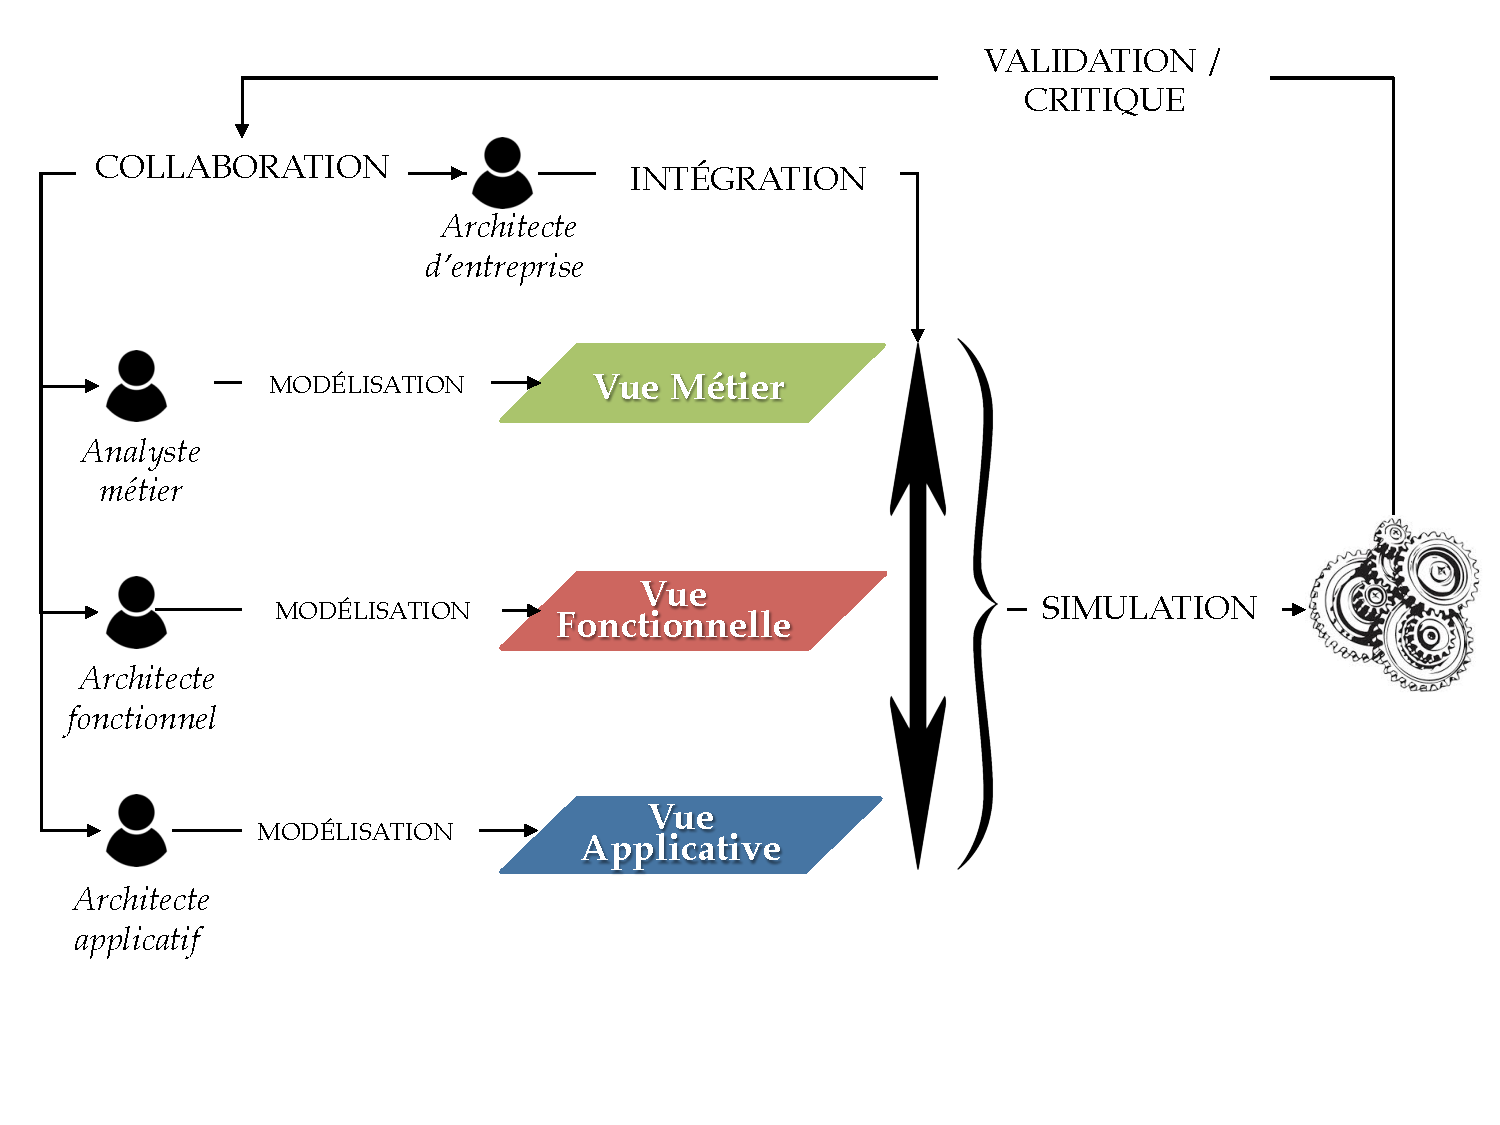
\includegraphics[trim= 0cm 3.5cm 0cm 0cm, 
width=1\textwidth]{figures/4_demarche/approche_conceptuelle.pdf}
 \end{center}
 \caption{Approche conceptuelle pour l'analyse d'une architecture d'entreprise}
 \label{fig:approche_conceptuelle}
\end{figure}

L'analyste métier, l'architecte fonctionnel et l'architecte applicatif 
collaborent entre eux et avec l'architecture d'entreprise pendant tout le 
processus de modélisation. Par la suite, l'activité d'intégration incombe à 
l'architecte d'entreprise, détenteur de la vision globale. Mais l'intégration 
des vues implique de rebouclage avec les autres acteurs (analyste métier, 
architecte fonctionnel et architecte applicatif) pour garantir l'alignement 
business/IT. Les étapes de modélisation et d'intégration de notre approche 
répondent donc aux objectifs de conception et de communication tels que définis 
par Kurpjuweit et Winter \cite{kurpjuweit2007viewpoint}.

Comme relaté dans l'état de l'art, l'analyse fait partie des activités les moins 
courantes de l'EA quelle qu'en soit l'école de pensée 
\cite{chen2008architectures} \cite{barn2013enterprise}. Et même lorsqu'une 
architecture d'entreprise est analysée très peu d'approches recourent à la 
simulation pour analyser l'aspect comportemental \cite{glazner2011enterprise} 
\cite{manzur2015xarchimate}. La simulation est pourtant une technique reconnue 
pour évaluer le comportement d'un système et/ou évaluer plusieurs stratégies 
concernant son fonctionnement \cite{shannon1975systems}. Notre approche 
préconise de simuler les modèles issus de activités de modélisation et 
d'intégration afin de les valider ou les critiquer par l'ensemble des acteurs 
impliqués dans l'EA. Nous couvrons ainsi l'objectif d'analyse tel que préconisé 
par Kurpjuweit et Winter \cite{kurpjuweit2007viewpoint}. 



\section{Un cadre d'architecture dirigé par les modèles exécutables}

\subsection{Approche par points de vue}

Toute simulation d'un système commence par sa modélisation. Pour modéliser des 
systèmes complexes comme les architectures d'entreprise, nous adoptons une 
approche par points de vue. Celle-ci facilite la conception des modèles par les 
acteurs impliqués en séparant leurs préoccupations respectives. Elle permet 
également de présenter les modèles obtenus, ainsi que les résultats de 
simulation de manière plus compréhensible à ces acteurs, car chaque point de vue 
n'utilise que les concepts métier propres à chaque acteur, selon sa perspective. 

Dans notre approche, nous nous intéressons aux vues métier, fonctionnelle et 
applicative comme l'illustre la figure~\ref{fig:vue_aspect}. Mais nous 
souhaitons aussi étendre nos travaux à la vue technique. 
Plusieurs raisons motivent l'utilisation de ces points de vue. D'abord, la vue 
métier et la vue applicative sont incontournables pour n'importe quel cadre 
d'architecture. Ensuite, selon les cadres d'architecture, la vue fonctionnelle 
est modélisée de deux manière~:~ elle est soit intégrée à la vue applicative 
sous forme de services (Archimate, TOGAF, RM-ODP), soit modélisée à part entière 
dans une vue dédiée (Club Urba, SGAM, Zachman). Nous prenons le parti de 
modéliser explicitement les fonctions dans une vue dédiée. En effet, passer 
directement de la vue du métier à la vue applicative peut être en quelque sorte 
brutal pour l'analyste métier mais aussi pour l'architecte applicatif. La vue 
fonctionnelle permet une transition progressive de la logique métier vers 
l'architecture logicielle.

Nous ne modélisons pas les informations dans une vue dédiée contrairement aux 
cadre RM-ODP ou SGAM. Nous explicitons les informations en tant qu'aspect pour 
chacune des autres vues comme recommandé par le cadre Zachman (Le quoi de la 
dimension horizontale). L'aspect «~\textit{information}~» permet d'avoir un 
modèle explicite des données utilisées dans chacune des vues métier, 
fonctionnelle et applicative :
	\begin{itemize}
	\item \textbf{L'aspect information du point de vue métier}
	
	Cet aspect établit le modèle de données métier qui  décrit les objets ou 
concepts métier manipulés par le processus métier. Ce modèle est peu sujet au 
changement, sauf évolution importante des pratiques métier. Il est aussi à 
l'origine du découpage en bloc par entité métier de la vue fonctionnelle~;
	\item \textbf{L'aspect information du point de vue fonctionnel}
	
	Cet aspect établit le modèle de données fonctionnelles qui donne le type des 
données utilisées par les blocs fonctionnels nécessaires à la réalisation de 
processus métier. Elle décrit leurs caractéristiques et leurs relations sous 
forme de diagrammes de classes par exemple~;
	
	\item \textbf{L'aspect information du point de vue applicatif} 
	
	Cet aspect établit le modèle de données applicatives qui dépend fortement des 
applications choisies : il décrit les formats de données compatibles avec les 
modules applicatifs.
	\end{itemize}
	
\begin{figure}[!ht]
 \begin{center}
  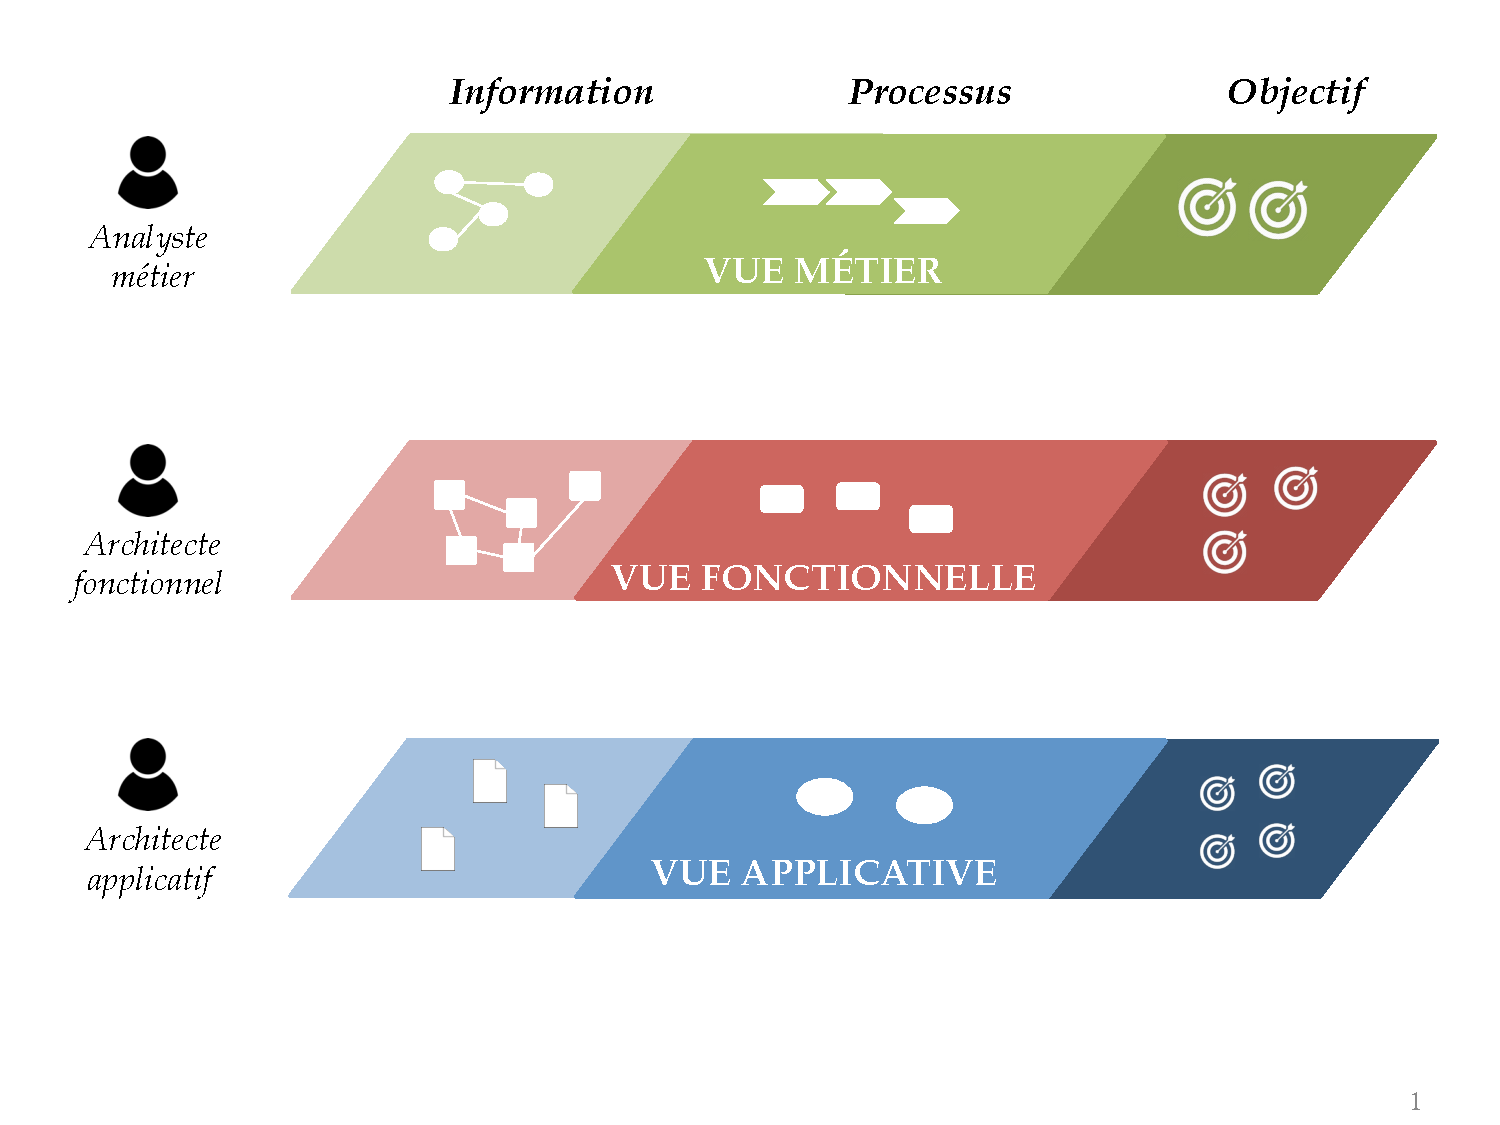
\includegraphics[trim= 0cm 3cm 0cm 0cm, 
width=1\textwidth]{figures/4_demarche/vue_aspect.pdf}
 \end{center}
 \caption{Points de vue et aspects utilisés}
 \label{fig:vue_aspect}
\end{figure}
	
De plus, nous modélisons le comportement de chaque vue dans l'aspect 
«~\textit{processus}~». Ainsi nous retrouvons~:

	\begin{itemize}
	\item \textbf{L'aspect processus du point de vue métier} 
	
	Cet aspect correspond aux processus métier de l'entreprise, décrits en 
utilisant les concepts métier, sans référence aux détails d'implémentation. Nous 
préconisons l'utilisation de formalismes standard pour la modélisation de 
processus métier qui soient exécutables, tels que les diagrammes d'activité fUML 
ou les diagrammes BPMN dans une perspective de simulation. Des langages 
spécifiques à un domaine (DSML) peuvent également être utilisés~;
	\item \textbf{L'aspect processus d'un point de vue fonctionnel} 
	
	Cet aspect décrit les fonctions qui réalisent les processus métier ainsi que 
leur orchestration en tant que processus fonctionnels. Ces fonctions sont 
regroupées en blocs. Chaque objet métier identifié dans l'aspect Information de 
la vue métier correspond à un unique bloc fonctionnel. Ceci garantit la 
construction de blocs fonctionnels fortement décorrélés, avec une forte cohésion 
interne. Dans chaque bloc fonctionnel, on retrouve les opérations correspondant 
à une tâche donnée du processus qui impacte l'objet métier impliqué~;
	\item \textbf{L'aspect processus du point de vue applicatif}
	
	Cet aspect décrit les modules logiciels qui implantent les blocs fonctionnels 
ainsi que leur orchestration en processus applicatifs. Dans un premier temps, il 
est conseillé de dresser un inventaire de l'existant applicatif et d'en extraire 
les modules capables de réaliser les opérations des blocs fonctionnels. Ensuite, 
si aucune application ou module existant ne peut répondre au besoin des nouveaux 
processus métier, l'architecte technique fait le choix des nouveaux composants 
applicatifs à mettre en place. En plus d'identifier les composants applicatifs 
existants ou à développer, l'architecte applicatif spécifie leurs 
interconnexions tels que échange de messages, synchronisation de données, 
transfert de fichiers périodique.
	\end{itemize}
	
Nous étendons chacune des vues par l'aspect «~\textit{objectif}~». Cet aspect 
correspond au «~\textit{pourquoi}~» du cadre Zachman qui spécifie les 
motivations de l'architecture. D'une part, modéliser cet aspect permet de garder 
une traçabilité d'une entre les processus modélisés et les objectifs qu'ils sont 
censés remplir. D'autre part, il permet de décliner les objectifs métier en 
objectifs applicatifs, et les objectifs applicatifs en objectifs fonctionnels. 
Comme nos travaux adoptent l'école de pensée «~Architecture du Système 
Entreprise~», nous souhaitons évaluer non seulement la composante SI mais 
l'ensemble de l'entreprise dont la stratégie. L'aspect objectif est un moyen de 
modéliser explicitement la stratégie de l'entreprise, traduite en un ensemble 
cohérent d'objectifs métier et ce pour évaluer la capacité des processus mis en 
place à y répondre et pour évaluer la stratégie elle-même par rapport à la 
réalité de l'entreprise. 

\subsection{Intégration d'une architecture d'entreprise} 

L'alignement et la cohérence sont des problématiques centrales en EA 
\cite{kaisler_enterprise_2005}. Notre contribution essentielle est de dédier un 
point de vue spécifique pour adresser ce type de problématique~:~le 
\textbf{point de vue intégration} illustré par la figure 
\ref{fig:vue_integration}. Ce point de vue définit un \textit{mapping} 
d'alignement en spécifiant (1)~les entités à aligner, (2)~les liens de cohérence 
entre ces éléments et (3) les transformations de modèles nécessaires au 
raffinement des ces entités. Les transformations de modèles facilitent et 
automatisent les passages d'une vue à l'autre. Ce point de vue permet une 
intégration «~IntraVue~» et «~InterVues~» (entres les aspects d'une seule vue). 
La figure \ref{fig:metamodele_framework} donne un métamodèle de notre framework 
en explicitant les concepts abordés et leurs relations.

\begin{figure}[!ht]
 \begin{center}
  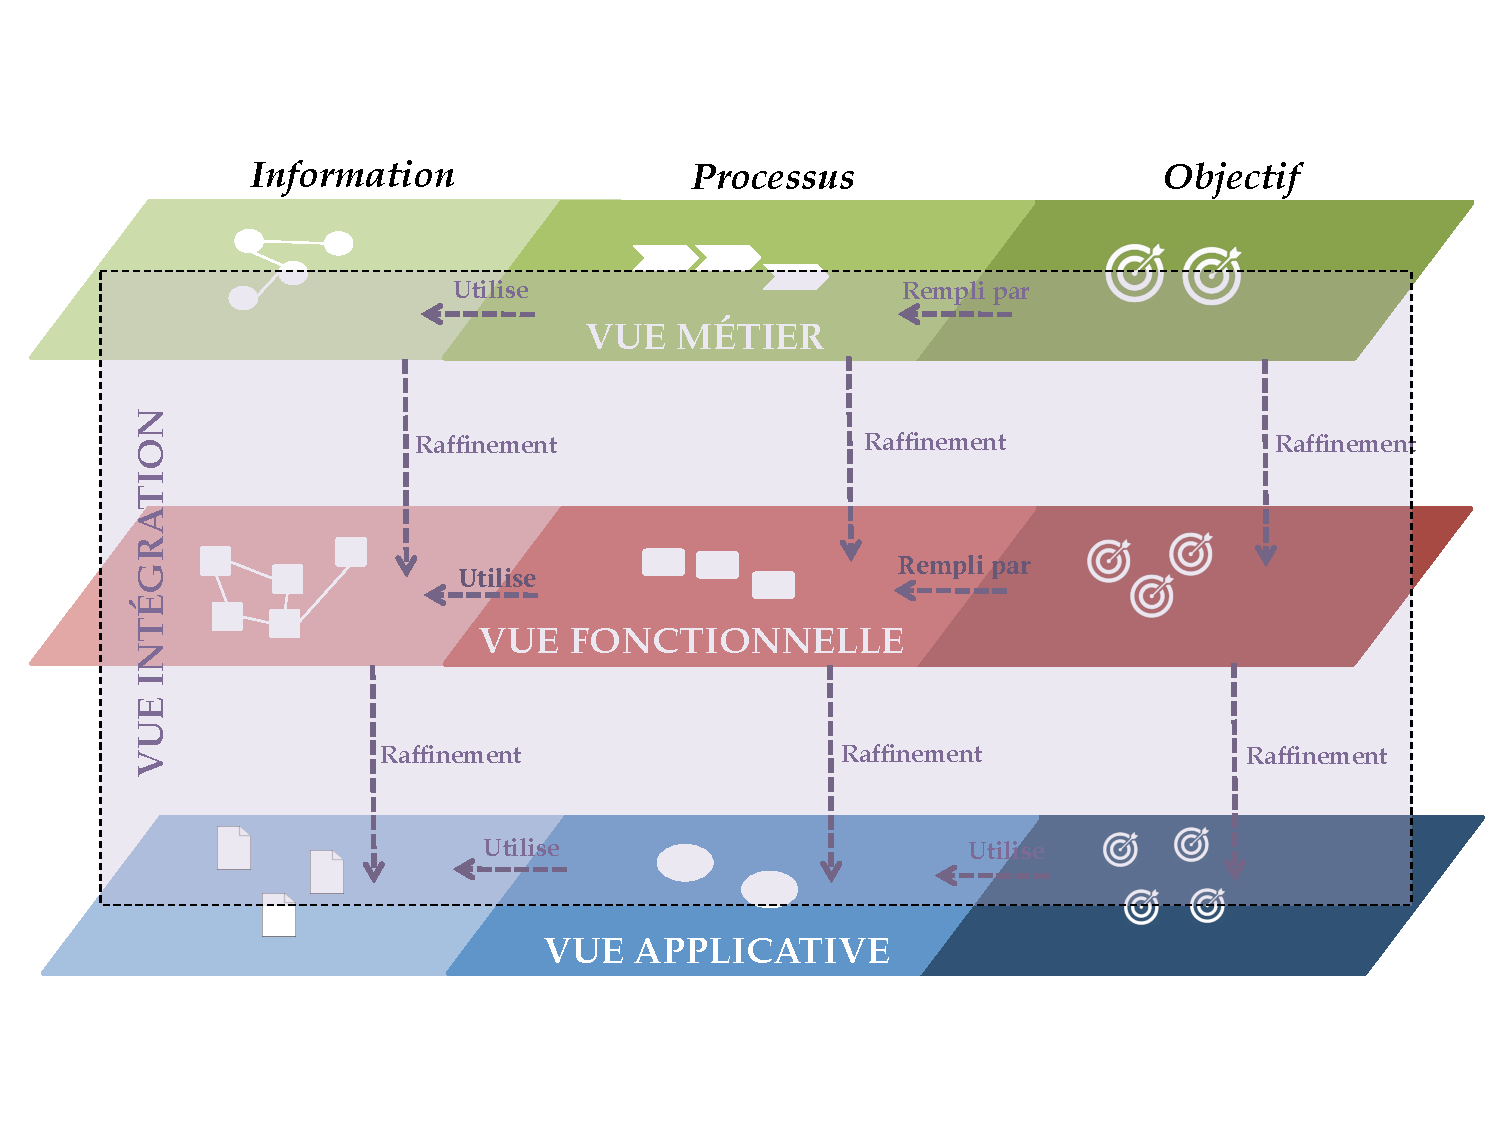
\includegraphics[trim= 3cm 3cm 0cm 0cm, 
width=1\textwidth]{figures/4_demarche/vue_integration.pdf}
 \end{center}
 \caption{Framework proposé avec la vue Intégration}
 \label{fig:vue_integration}
\end{figure}

L'intégration inter-vues décrit les relations entre les vues (sauf la vue 
intégration). La vue intégration est donc transverse à toutes les autres vues et 
permet de modéliser explicitement les notions de raffinement à travers la classe 
«~InterVues~» (voir figure \ref{fig:metamodele_framework}), tant pour  les 
aspects \emph{processus} et \textit{information} que sur les aspects 
\emph{objectif}.

\begin{figure}[!ht]
 \begin{center}
  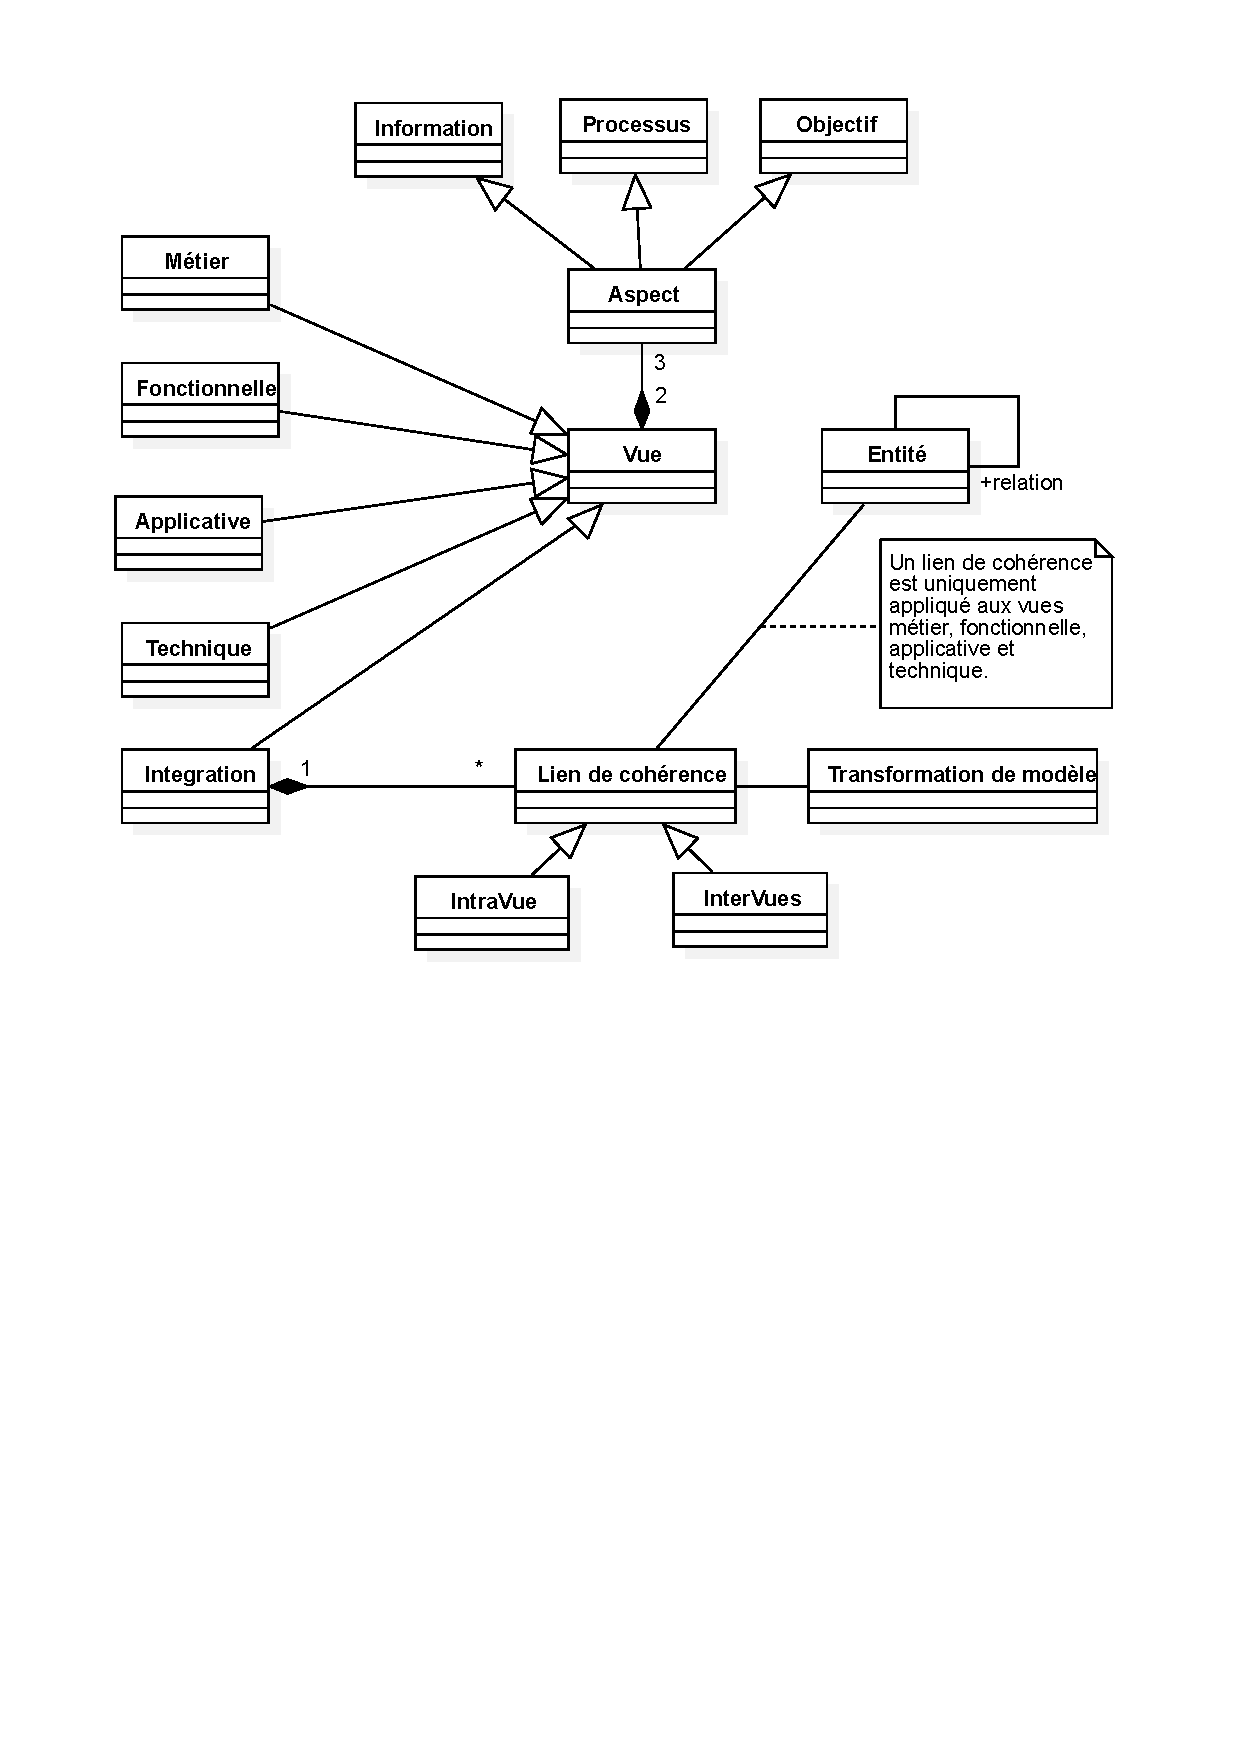
\includegraphics[trim= 0cm 13cm 0cm 2cm, 
width=1\textwidth]{figures/4_demarche/metamodele_framework.pdf}
 \end{center}
 \caption{Métamodèle du framework proposé}
 \label{fig:metamodele_framework}
\end{figure}

Nous donnons le métamodèle de la vue intégration dans la figure 
\ref{fig:metamodele_vue_integration}. Cette vue permet des vérifications 
horizontales à l'intérieur de chacune des vues. En effet, l'association 
«~utilise~» assure donc la compatibilité des données échangées entre les tâches 
d'un processus métier, les fonctions d'un bloc fonctionnel ou entre les modules 
d'une application (voir figure \ref{fig:metamodele_vue_integration}). 
L'association «~rempli par~» hérite aussi de la classe «~IntraVue~» et associe 
explicitement une entité à l'objectif qui lui est assigné. De cette manière, il 
est possible de tracer l'implémentation effective d'une stratégie métier à 
travers l'ensemble de l'entreprise, des entités métier à l'IT.

La définition d'un métamodèle précis pour le framework permet de plus de 
contrôler la conformité des modèles d'architecture. Ainsi, une entité du modèle 
(telle qu'une fonction, une tâche du processus métier, un objectif, etc.) 
appartient toujours à deux vues~:~une vue intégration en plus d'une autre vue 
parmi les vues métier, fonctionnelle, applicative et technique. Autre exemple, 
tous les objectifs de la vue métier doivent avoir des liens de cohérence 
inter-vues avec les objectifs de la vue fonctionnelle et de même pour ces 
dernier avec les objectif de la vue applicative et ainsi de suite. De même pour 
les autres entités des aspects information et processus. Une fois le modèle 
d'architecture créé, il est possible de vérifier sa conformité au métamodèle et 
de s'assurer que la cohérence entre les différentes entités de modèles est bien 
maintenue. 

La vue intégration permet en outre de vérifier qu'une application implémente 
bien tous les blocs fonctionnels nécessaires au déroulement d'un processus 
métier. Cette vue donne ainsi accès aux informations de traçabilité qui 
permettent de déterminer l'impact d'une modification ou d'une défaillance d'un 
module applicatif sur les processus métier. Elle permet aussi de vérifier que 
les formats applicatifs permettent d'encoder les types de données fonctionnelles 
requis, qui eux-même raffinent les concepts métiers. Cette vue détermine les 
éventuelles transformations de modèle nécessaires au déploiement en spécialisant 
l'association «~raffine~». Le choix des modèles à transformer dépend fortement 
de leur nature (modèles graphiques, textuels, etc.) et mais aussi de leur niveau 
d'abstraction. Par exemple, la génération de code demande un modèle en entrée 
suffisamment détaillé pour exécuter une transformation pertinente. L'état de 
l'art actuel des langages de transformation de modèle privilégie l'usage des 
transformations de modèle entre la vue fonctionnelle et et la vue applicative. 


\begin{figure}[!ht]
 \begin{center}
  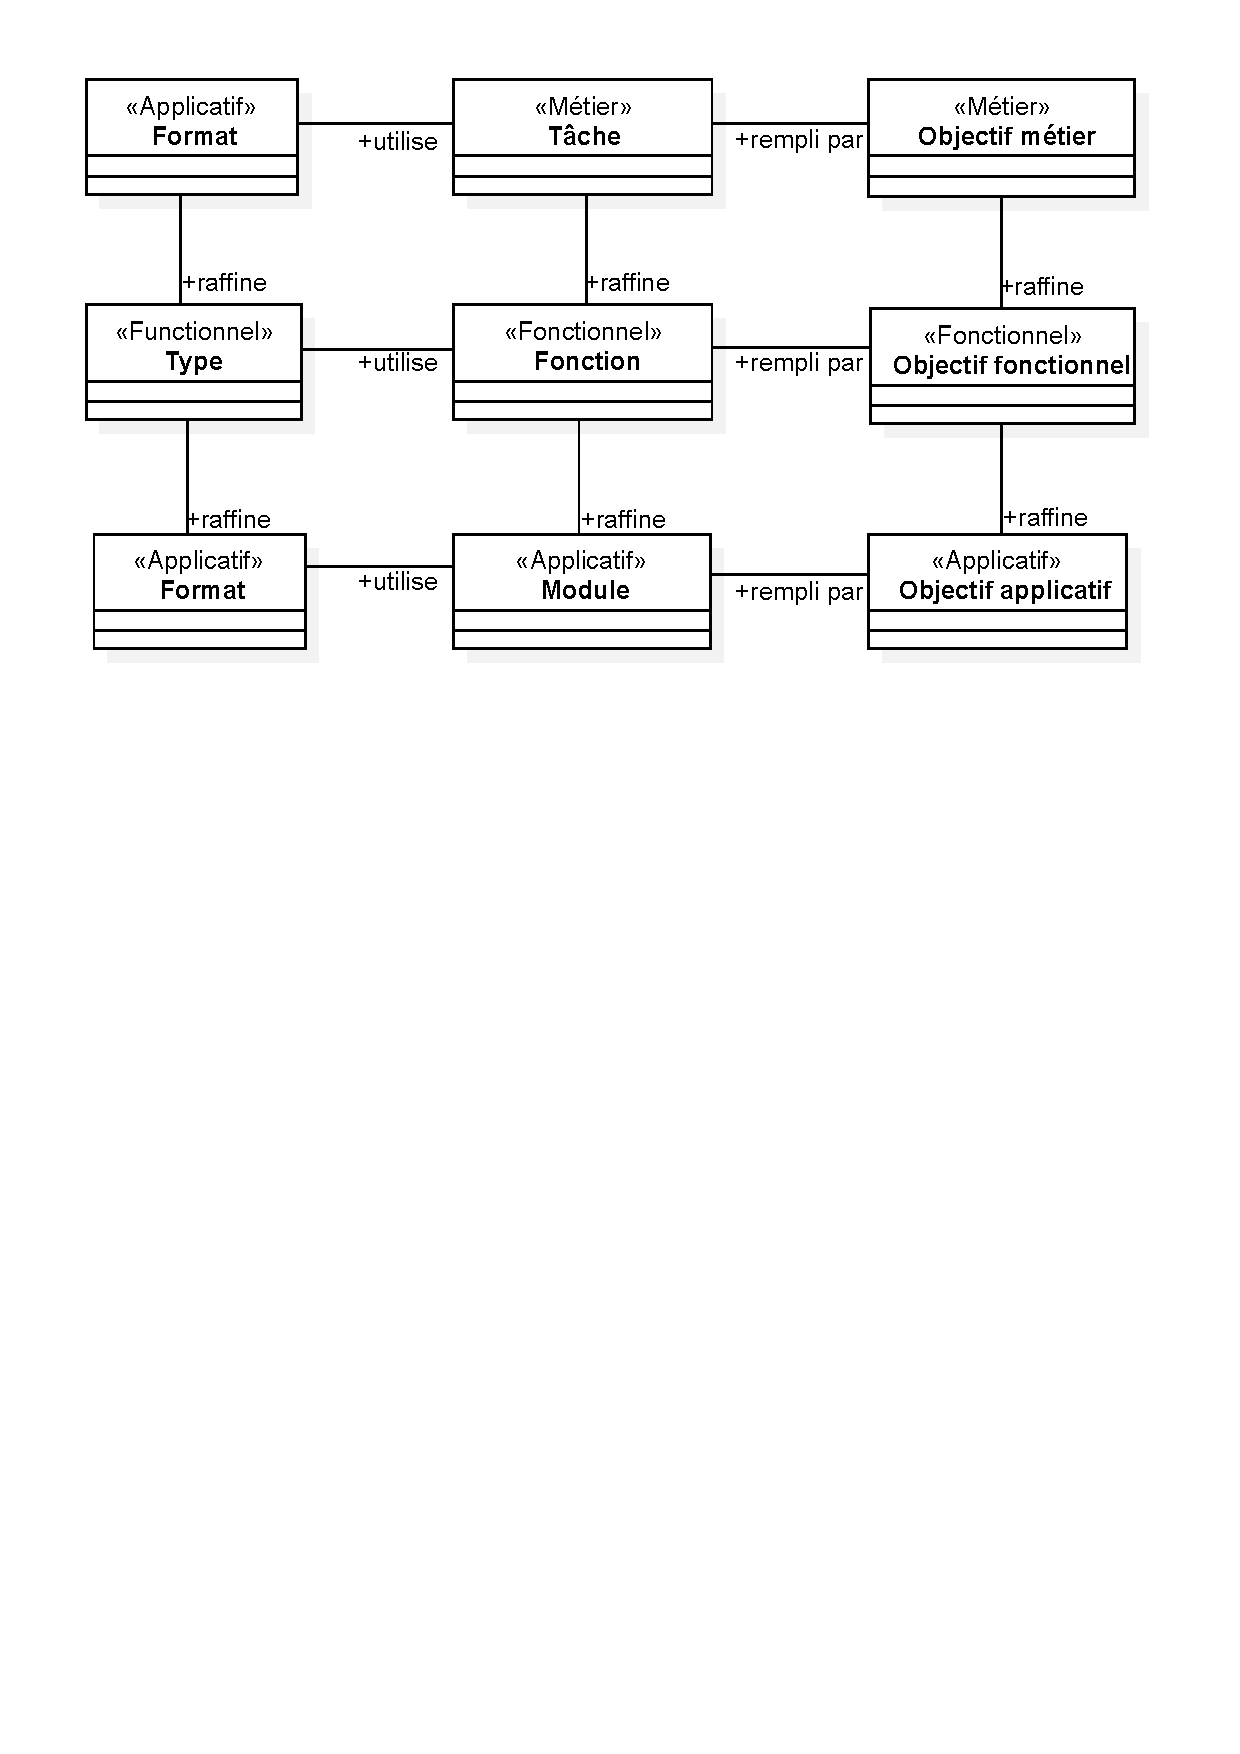
\includegraphics[trim= 0cm 18cm 0cm 0cm, 
width=1\textwidth]{figures/4_demarche/metamodele_vue_integration.pdf}
 \end{center}
 \caption{Métamodèle de la vue intégration}
 \label{fig:metamodele_vue_integration}
\end{figure}


\subsection{Analyse de l'architecture d'entreprise}

\subsubsection{Analyse du comportement : simulation dirigée par les processus 
métier}

Pour simuler le comportement d'une entreprise nous nous appuyant sur les modèles 
d'architecture d'entreprise préalablement définis par les différentes parties 
prenantes. L'EA permettent de capturer l'essentiel des composants d'une 
entreprise sous forme d'abstraction. Une approche par points de vue guide la 
décomposition d'une entreprise en vues pertinentes pour les différents acteurs. 
Ces vues apportent une aide supplémentaire à la définition du périmètre des 
modèles de simulation. La vue intégration permet en particulier de définir les 
liens entres les différentes vues, donc entre les différents modèles de 
simulation et de garantir la cohérence et donc la pertinence de la simulation. 
Comme les modèles de simulation sont directement dérivés de l'architecture 
d'entreprise telle qu'elle est définie par les parties prenantes, elle est 
d'autant plus facile à appréhender à comprendre. Ces derniers peuvent aussi 
aisément communiquer et échanger autour des résultats de la simulation. 

Les modèles d'entreprise doivent offrir un niveau d'abstraction suffisant à la 
compréhension, l'analyse et la communication. Les modèles doivent donc permettre 
d'abstraire les détails techniques et les nombreuses interconnexions tout en 
garantissant la traçabilité et la cohérence de l'ensemble de l'architecture. 
Notre approche consiste donc de mettre en lumière les composants et les 
relations qui sont critiques pour le comportement de l'ensemble de 
l'architecture. En effet, modéliser l'architecture d'une entreprise revient à la 
modélisation de systèmes complexes. Herbert Simon \cite{simon1990prediction} 
dans ses travaux de modélisation de systèmes complexes affirme que 
«~l'approximation judicieuse et non la puissance de calcul d'une machine~» reste 
la manière la plus effective d'adresser des systèmes complexes.

La simulation des processus métier est souvent réduite à de la simple animation 
visuelle de diagrammes pour vérifier l'orchestration des taches métier. Nous 
proposons de piloter la simulation du comportement de l'architecture par le 
processus métier. Dans ce cas, le calcul d'une valeur ne se fait pas au niveau 
de la tache métier mais du module applicatif qui l'implémente. Le processus 
métier est modélisé sous forme de diagrammes d'activité fUML. Dans ce cas les 
simulations du comportement de l'architecture d'entreprise est pilotée par les 
processus métier qui sont alors responsable d'orchestrer l'ensemble des modèles 
comme l'illustre la figure \ref{fig:Simulation_Approche}. La simulation est 
lancée après l'intégration de l'architecture à travers la création de lien de 
cohérences intra-vue et inter-vues. Ces liens sont par la suite utilisés pour 
mettre en œuvre la simulation. D'une part, la \textit{Tâche~A} de la figure 
\ref{fig:Simulation_Approche} appelle le \textit{Module~A} car le 
\textit{Module~A} raffine la \textit{Fonction~A} qui elle-même raffine la 
\textit{Tâche~A}. D'autre part, les liens de cohérences intravue garantisse une 
compatibilité entre les informations envoyés par la \textit{Tâche~A} et celles 
attendues par la \textit{Tâche~B}, de même entre la \textit{Fonction~A} et la 
\textit{Fonction~B} et entre le \textit{Module~A} et le \textit{Module~B}.

\begin{figure}[!ht]
 \begin{center}
  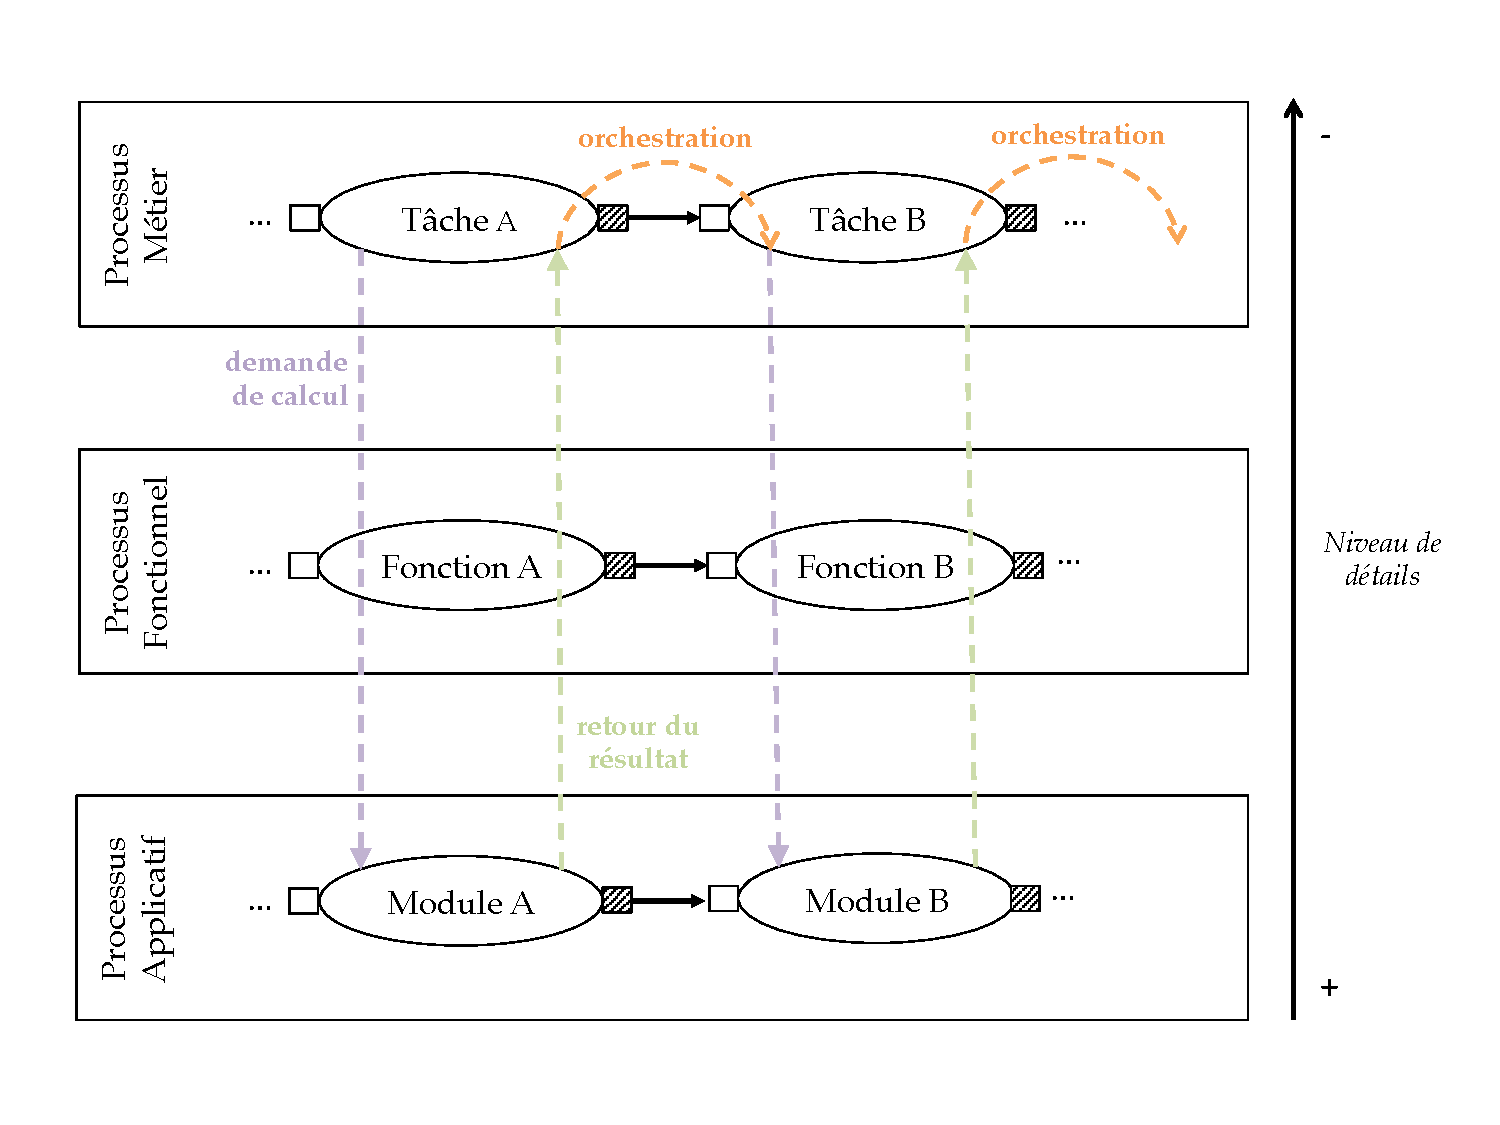
\includegraphics[trim= 0cm 2cm 0cm 0cm, 
width=1\textwidth]{figures/4_demarche/approche_simulation.pdf}
 \end{center}
 \caption{Simulation dirigée par les processus métier}
 \label{fig:Simulation_Approche}
\end{figure}

En plus de s'appuyer sur les processus métier pour piloter la simulation de 
l'ensemble du comportement de l'architecture d'entreprise, notre approche 
consiste à mettre à profit les techniques et les langages de l'IDM pour 
faciliter l'automatisation de l'activité d'analyse du comportement. Nous nous 
appuyant sur le manifeste de IBM \cite{chesbrough2006research} concernant l'IDM 
dans la sélection de techniques et langages qui soient pertinents pour notre 
approche. Le manifeste de IBM recommande l'utilisation de langages 
(1)~exécutables, (2)~standardisés et (3) compréhensibles par les experts du 
domaine. C'est le cas de fUML, BPMN et OCL. La figure \ref{fig:IDM_EA} fait la 
correspondance entre les langages et la possibilité de les utiliser selon les 
vues. 


Ces langages permettent une exécution directe des modèles créés. Contrairement à 
d'autres méthodes de simulation de processus métier qui utilisent l'IDM pour 
isoler la définition du processus de son exécution. Ces méthodes font ensuite 
appel aux transformations de modèle pour automatiser la conversion entre les 
modèles de représentation et leur exécution. 

\begin{table}[!ht]
    \begin{center}
        \setlength{\mytablewidth}{0.8\textwidth}
\setlength{\mycolwidth}{\dimexpr0.25\mytablewidth-2\tabcolsep\relax}

\begin{tabulary}{\mytablewidth}{m{\mycolwidth}m{\mycolwidth}m{\mycolwidth}m{\mycolwidth}}
\cmidrule[\heavyrulewidth]{2-4}

                        & \centbf{Metier}       & \centbf{Fonctionnel}  & \centbf{Applicatif}   \tabularnewline\midrule
    \centbf{BPMN}       & \center{\checkmark}   &                       &                       \tabularnewline
    \centbf{fUML}       & \center{\checkmark}   & \center{\checkmark}   &                       \tabularnewline
    \centbf{OCL}        &                       & \center{\checkmark}   &                       \tabularnewline
    \centbf{MiniZinc}   &                       &                       & \center{\checkmark}   \tabularnewline

\bottomrule
\end{tabulary}

    \end{center}
    \caption{Langages de l'IDM pour l'EA}
    \label{fig:IDM_EA}
\end{table}

\subsubsection{Analyse de la structure}
Tout comme l'analyse du comportement, l'analyse de la structure de 
l'architecture d'entreprise est étroitement lié à l'impératif de cohérence.  Il 
est indispensable s'assurer de la cohérence entres les modèles des différentes 
vues avant d'initier une analyse structurelle qui soit pertinente pour les 
parties prenantes et en particulier pour l'architecte d'entreprise. 

Notre contribution consiste à définir la manière dont les langages et techniques 
de l'IDM peuvent être utilisés pour mener une analyse structurelle des modèles 
d'entreprise. Le cadre d'EA que nous proposons permet d'acquérir une vision 
globale et cohérente de l'ensemble des artefacts qui la composent. La taille de 
plus en plus importantes des entreprises actuelle fait que la complexité de 
l'entreprise en tant que système se retrouve dans les modèles d'architecture qui 
le représentent.

L'analyse automatisée de ces modèles facilite leur appréhension par l'acteur qui 
mène ces analyses (en l'occurrence l'architecte d'entreprise). Elle permet de 
révéler la structure de l'entreprise et le fonctionnement de cette structure. Un 
intérêt  typique de l'analyse de la structure est la mesure de l'impact du 
changement \cite{de2005change} sur l'architecture. L'analyse de l'impact du 
changement consiste à dévoiler les effets de bord d'un changement apporté à un 
élément de l'architecture.  

Les langages de modélisation doivent donc permettre de représenter 
convenablement les différents composants de l'entreprise en plus d'offrir la 
possibilité d'analyser la structure des modèles créés dans l'objectif de mieux 
comprendre le système réel, qui est dans ce cas l'entreprise. Nous proposons 
donc de tirer profit des méthodes IDM telle la métamodélisation et de les 
associer à des langages capables d'exprimer et d'exécuter des contraintes et des 
requêtes sur les modèles tels que OCLinEcore ou QVT. Grâce à ce type de langage 
il est possible de~:
\begin{enumerate}
\item modéliser des règles de structure supplémentaires qui précisent d'avantage 
méta-modèle d'architecture. Une fois que le modèle d'architecture est conforme à 
ce métamodèle, il est possible de vérifier qu'il respecte bien toutes les 
contraintes exprimées au niveau du métamodèle~;
\item analyser l'impact du changement pour évaluer par exemple l'impact de 
l'indisponibilité d'un module applicatif sur l'architecture globale. En mettant 
à profit les liens de cohérence de la vue intégration, il est alors possible de 
déterminer quels sont les processus métier ou fonctionnels touchés par cette 
défaillance applicative. De même, il est possible d'identifier les modules 
applicatifs existants pouvant participer à la réalisation d'un nouveau métier si 
ces processus fait intervenir des taches métier déjà implémentées dans le SI.
\end{enumerate}




 
%
%%(Describes the system’s functional elements, their responsibilities, 
%interfaces, and primary interactions. A Functional view is the cornerstone of 
%most ADs and is often the first part of the description that stakeholders try 
to 
%read. It drives the shape of other system structures such as the information 
%structure, concurrency structure, deployment structure, and so on. It also has 
a 
%significant impact on the system’s quality properties such as its ability to 
%change, its ability to be secured, and its runtime performance.)
%
%%\subsubsection{Le Model Typing pour la cohérence inter- et intra-vue}
%%Le \textit{Model Typing} est une technique de l'IDM appliqué au développement 
%logiciel permettant de contrôler les types de modèles d'entrée des 
%transformations de modèle à leur exécution. Nous proposons d'appliquer les 
%principes du \textit{Model Typing} aux modèles d'EA et aux transformations de 
%modèle qui leurs sont associées. Par exemple, un processus métier utilise en 
%entrée et en sortie des modèles représentant des concepts métier. Un processus 
%peut donc être considéré comme une transformation de modèle. 
%%Ainsi, le \textit{Model Typing} peut être utilisé pour l'intégration 
%horizontale (i.e. cohérence et orchestration des processus d'une même vue). 

	%!TEX  root = main.tex
\chapter{Prototypage et validation du \emph{framework ExecuteEA}}
\label{ch:implem}

\PartialToc


\section{Environnement retenu : la plate-forme Eclipse}

Notre choix s'est orienté vers la plate-forme Eclipse et ce pour plusieurs
raisons.

Tout d'abord, il s'agit d'une plate-forme open-source dont l'utilisation est
particulièrement répandue dans la communauté IDM. En effet, la plate-forme
Eclipse abrite le projet
\gls{emf}\footnote{http://www.eclipse.org/modeling/emf/} qui a pour objectif de
doter Eclipse d'outils orientés IDM.

Ensuite, \gls{emf} s'appuit sur les standards du domaine. Par exemple, le méta-
métamodèle Ecore, pilier central de \gls{emf}, se base sur le standard
\gls{mof}\footnote{http://www.omg.org/mof/} . Aure exemple, le langage de
contraintes OCLinEcore se base sur le standard \gls{ocl}. OCL et MOF sont des
standard de l'OMG.

Puis, \gls{emf} se décompose en sous-projets orientés vers différents aspects de
l'IDM tels que la méta-modélisation, la transformation de modèle, les éditeurs
graphiques de modèles, les langages spécifiques au domaine. \gls{emf} offre
ainsi un environnement personnalisable pour mettre en œuvre une approche IDM.

Enfin, il s'agit de la plate-forme retenu par le projet Pomme du département
MIRE, dans lequel s'inscrit nos travaux de thèse. Le projet Pomme vise à
réaliser un outil pour la co-simulation des trois domaines qui compose un Smart
Grid~: SI, infrastructure électrique, infrastructure de télécommunication.

Pour ces travaux de thèse, nous avons donc retenu~:

\begin{itemize}

    \item Ecore pour la méta-modélisation~;

    \item OCLinEcore pour l'expression de contraintes et de requêtes sur le métamodèle~;

    \item Le langage Acceleo pour les transformations de modèle~;

    \item Le plugin Papyrus\footnote{https://eclipse.org/papyrus/} pour la simulation
    des modèles d'architecture. Papyrus est compatible avec le standard fUML et
    permet donc d'exécuter les diagrammes de classes et d'activité. 

\end{itemize}


\section{Réalisation et difficultés rencontrées}

    \subsection{Implémentation du métamodèle EA2M avec Eclipse Modeling Framework}

    Le métamodèle EA2M est le pilier central du \emph{framework ExecuteEA}. Nous
    l'avons implémenté à l'aide de \gls{emf}. Il est donc conforme au méta-
    métamodèle Ecore. EMF génère automatiquement un éditeur de modèle à partir
    d'un métamodèle conforme à Ecore. Cet éditeur permet de créer des modèles
    d'architecture d'entreprise conformes au métamodèle EA2M ainsi implémenté.
    La figure~\ref{fig:editeur_modele1} et la figure~\ref{fig:editeur_modele2}
    sont une capture d'écran de l'éditeur de modèles générée automatiquement à
    partir du métamodèle EA2M. L'utilisateur a le choix de créer une vue métier,
    fonctionnelle, applicative ou intégration et pour chacune des vues il peut
    choisir de créer un aspect objectif, processus ou information.


    \begin{figure}[!htbp]
     \begin{center}
      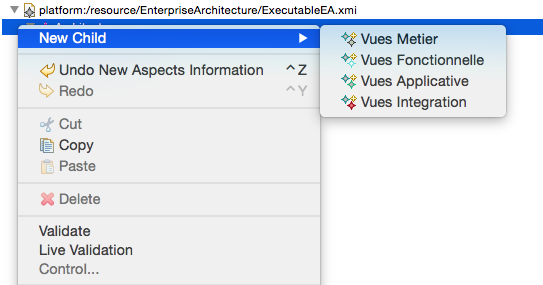
\includegraphics[width=0.8\textwidth]{figures/5_implementation/editeur_modele1.png}
     \end{center}
     \caption{Edition de modèles d'architecture d'entreprise avec ExecuteEA\\création de vues}
     \label{fig:editeur_modele1}
    \end{figure}

    \begin{figure}[!htbp]
     \begin{center}
      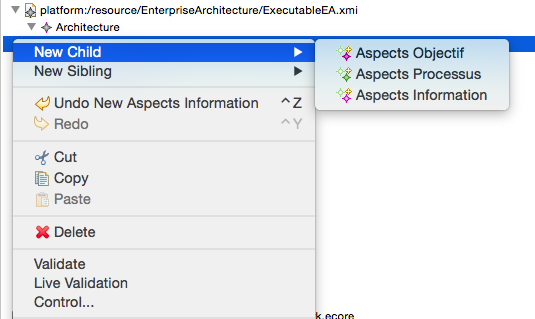
\includegraphics[width=0.8\textwidth]{figures/5_implementation/editeur_modele2.png}
     \end{center}
     \caption{Edition de modèles d'architecture d'entreprise avec ExecuteEA\\création d'aspects}
     \label{fig:editeur_modele2}
    \end{figure}

    La figure~\ref{fig:modeleEA} représente une capture d'écran d'un modèle d'architecture
    d'entreprise créé avec l'éditeur de modèle ExecuteEA.

    \begin{figure}[!htbp]
     \begin{center}
      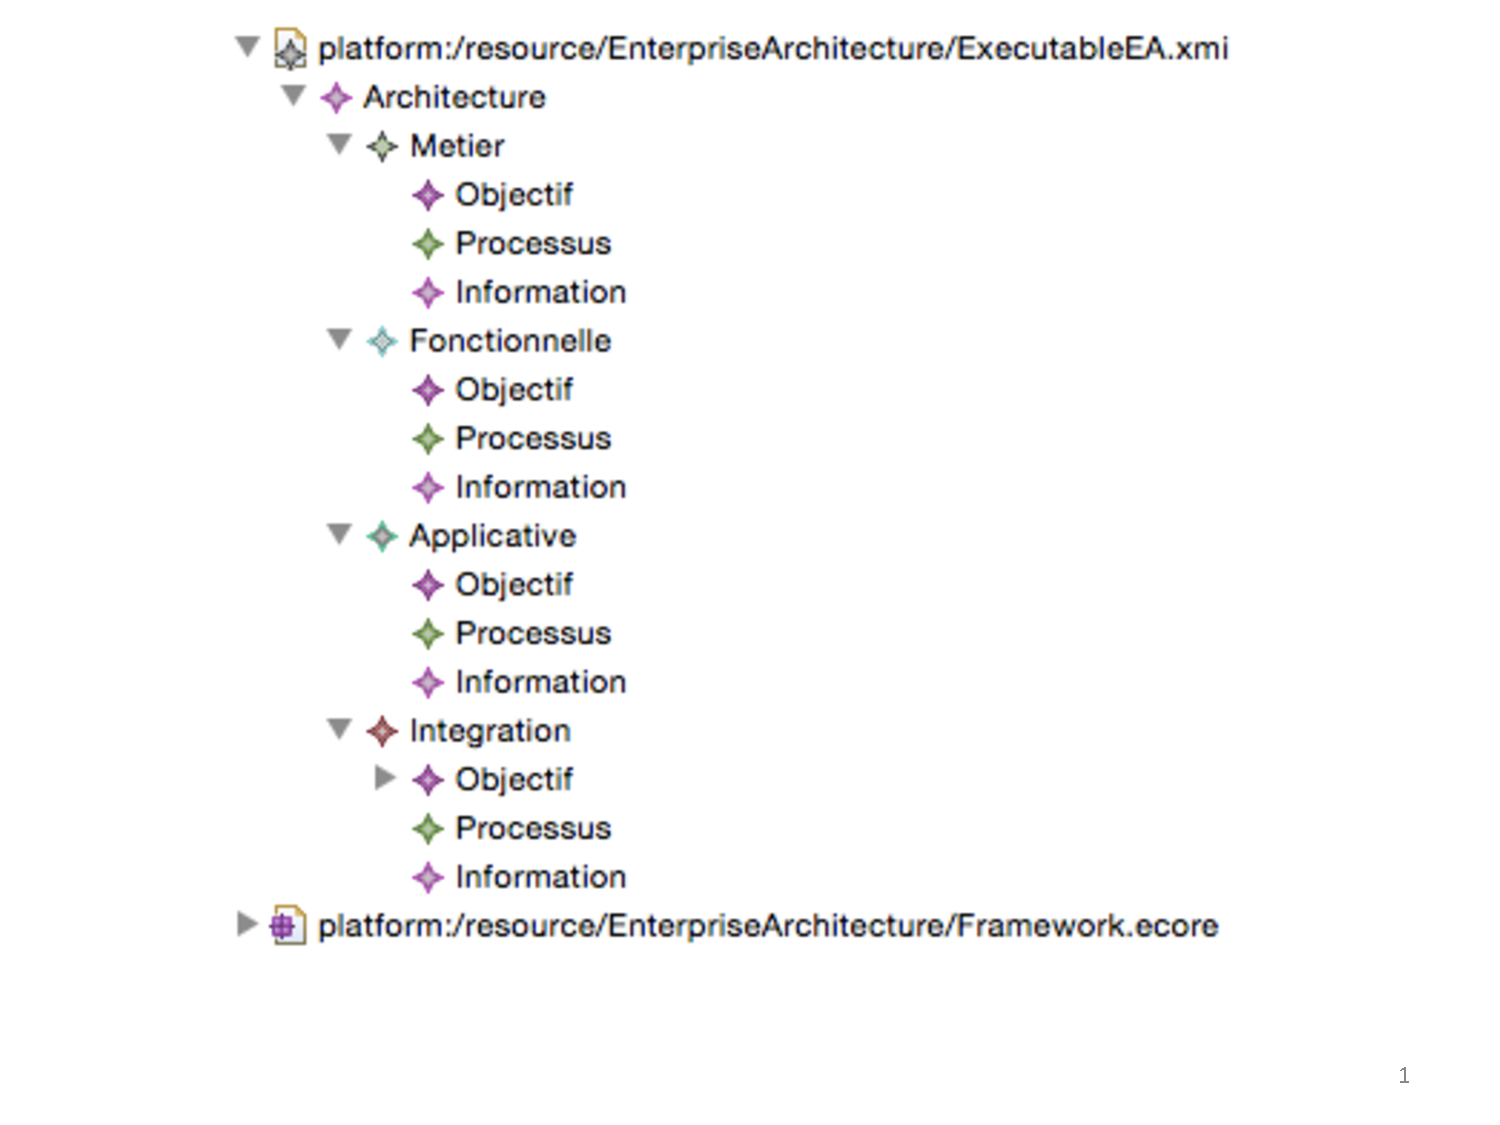
\includegraphics[trim=0cm 3cm 0cm 0cm, width=0.8\textwidth]{figures/5_implementation/modele_ea.pdf}
     \end{center}
     \caption{Modèle d'architecture d'entreprise créé avec l'éditeur ExecuteEA}
     \label{fig:modeleEA}
    \end{figure}

    La difficulté majeure rencontrée en implémentant le métamodèle EA2M a été de
    trouver le bon équilibre entre deux impératifs~: (1) implémenter le
    métamodèle en utilisant des concepts et des relations qui font sens d'un
    point de vue EA, en se gardant la possibilité de l'étendre facilement,
    notamment, par d'autres aspects ou d'autres vues, (2) tout en créant un
    éditeur suffisamment contraignant pour créer des modèles d'architecture
    corrects. Par exemple, utiliser uniquement le mécanisme de multiplicités
    entre la classe abstraite \q{Vue} et la classe \q{Architecture} ne contraint
    pas le modélisateur à ne pas créer plusieurs fois le même type de vue pour
    une seule architecture. Un modèle avec deux vues métier serait par
    conséquent conforme au métamodèle mais ne serait pas pertinent d'un point de
    vue EA.

    Nous avons donc exprimé des contraintes avec OCLinEcore pour ne créer que
    des modèles pertinents tout en gardant un métamodèle pertinent d'un point de
    vue purement EA.  Une contrainte est une expression à valeur booléenne qui
    sert à préciser ou restreindre n'importe quel élément du métamodèle.

    La figure~\ref{fig:contraintes_ocl_architecture} illustre le métamodèle
    EA2M, implémenté à l'aide d'\gls{emf}, sous une forme textuelle\footnote{EMF
    est doté d'une éditeur graphique qui permet de créer des métamodèles de
    manière graphique (par \emph{drag and drop}) sous la forme d'un diagramme de
    classe et de générer le même métamodèle sous une forme textuelle.}. Il
    s'agit donc de la classe \q{Architecture} à la quelle on a ajouté des
    contraintes de type \q{invariant} pour qu'elle ne contiennent pas de vue du
    même type.

    \begin{figure}[!htbp]
     \begin{center}
      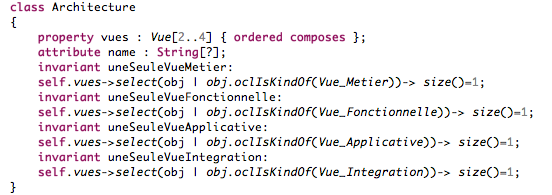
\includegraphics[width=0.8\textwidth]{figures/5_implementation/ocl_in_ecore_vue.png}
     \end{center}
     \caption{Contraintes OCLinEcore attachées à la classe \protect\q{Architecture} }
     \label{fig:contraintes_ocl_architecture}
    \end{figure}

    \subsection{Exécution des modèles d’architecture avec Papyrus}
    \label{sec:opaque_action_papyrus}

    Papyrus est un atelier de modélisation orienté IDM doté d'un moteur
    d'exécution de diagrammes fUML conformément aux spécifications de l'OMG.
    Nous l'avons utilisé pour simuler l'architecture. Comme présenté dans le
    chapitre~\ref{ch:proposition}, nous proposons de simuler l'ensemble de
    l'architecture en la pilotant par les modèles.  La difficulté majeure
    rencontrée à cette étape de l'implémentation a été de réussir à exécuter des
    comportements difficile à modéliser avec un diagramme
    UML\footnote{Typiquement, l'optimisation d'une affectation de véhicules
    électriques à des tournées d'agents qui intervient dans le cas d'études
    présenté dans la suite de ce chapitre}. Le principe de simulation pilotée
    par les processus métier, tel que présenté dans la
    figure~\ref{fig:Simulation_Approche}
    (page~\pageref{fig:Simulation_Approche}), exige de plus de faire appel aux
    modules de la vue applicative.
    
    Le standard fUML a prévu l'exécution de comportements spécifiques difficiles
    à modéliser avec  des diagrammes d'activité. Il dédie à cet effet une
    action\footnote{Dans les spécifications d'UML et de fUML, une action est une étape
    unitaire à l'intérieur d'une activité. Une activité est donc composée de
    plusieurs actions.} spécialisée~: l'\emph{OpaqueAction}. Papyrus s'appuie
    sur le moteur d'exécution Moka pour simuler les diagramme fUML. Moka est
    conforme à la sémantique d'exécution spécifiée par l'OMG pour fUML. Or la
    sémantique d'exécution de l'\emph{OpaqueAction} n'a pas encore été
    spécifiée. Le standard fUML est en effet relativement récent\footnote{La
    première version de fUML a été publiée par l'OMG en févier 2011} et n'a pas
    encore été entièrement spécifié. Pour cette raison, le moteur d'exécution
    Moka ne prend pas en charge l'exécution de l'\emph{OpaqueAction}

    Cependant, Papyrus donne la possibilité d'étendre le moteur d'exécution Moka
    et en attribuant le comportement souhaité à \emph{OpaqueAction} et en
    l'exécutant comme les autres actions au cours d'une simulation de diagramme
    d'activité. Cette extension n'a toutefois pas été facile à implémenter. Les
    tutoriels mis à disposition par l'équipe de développement du module Moka
    sont utiles pour une utilisation basique mais ne répondent à des besoins
    d'utilisation pointues telle que l'extension du moteur d'exécution
    disponible. À cet effet, nous avons sollicité l'aide de contributeurs au
    développement du module Moka et nous nous sommes également appuyé sur un
    stagiaire en dernière école d'ingénieur. Le comportement de
    l'\emph{OpaqueAction} mis en œuvre dans ces travaux de thèse consiste donc à
    appeler un module extérieur durant l'exécution d'un diagramme d'activité
    fUML et à retourner le résultat fourni par le module à l'action ou
    l'activité suivante.

    Dans la suite de ce chapitre, nous éprouvant le \emph{framework ExecuteEA}
    ainsi doté d'un environnement de modélisation et de simulation de modèles
    d'architecture. La validation est faite à travers le cas d'étude de la
    gestion d'une flotte de véhicules électrique. Nous avons créé à cet effet
    (1) les modèles d'architecture d'entreprise requis par les différentes vues
    et selon les aspects spécifié par \emph{ExecuteEA} en adoptant les langages
    prescrit par le \emph{framework}, et (2) les transformations de modèle
    nécessaires. Nous avons ensuite analyser l'architecture obtenue.


\section{Concrétisation de l'approche avec un cas d'étude}

    Les contraintes de temps et de confidentialité ne nous ont pas permis
    d'éprouvé le framework ExecuteEA sur une architecture d'entreprise à taille
    réelle. Pour cette raison, le cas d'étude concerne plutôt un seul processus
    métier faisant intervenir plusieurs tâches et sa déclinaison sur les vues
    fonctionnelle et applicative. Il s'agit de la gestion d'une flotte de
    véhicules électriques. Ce cas métier nous permet néanmoins de concrétiser
    les propositions de ces travaux de thèse et de parer à la difficulté
    d'évaluer quantitativement ces propositions.

    \subsection{Présentation du cas d'étude~:\\la gestion d'une flotte de véhicules électriques}

    Les raisons motivant le choix de ce cas d'étude pour éprouver le framework
    proposé dans ces travaux de thèse ont été discutées dans le
    section~\ref{motivations_cas_metier} (voir
    page~\pageref{motivations_cas_metier}).  Dans cette partie, nous nous
    contentons donc simplement de le présenter.

    Il s'agit du processus d'affectation de véhicules à des tournées d'agents
    (par exemple, une tournée d'un agent EDF qui relève les compteurs chez les
    client, ou encore qui fait des réparations le réseau électrique).  La
    mobilité électrique implique un changement de paradigme pour le gestionnaire
    de flotte de l'entreprise. D'une part, le véhicule électrique est limité par
    son autonomie et ne peut donc pas effectuer n'importe quelle tournée.
    D'autre part, la recharge d'un véhicule électrique implique des contraintes
    (temps de recharge, disponibilité des bornes) que ne présente pas le
    véhicule thermique qui se contente d'un plein de carburant.
    
    Dès lors, le processus d'affectation de véhicules aux tournées des agents,
    la gestion de la flotte de véhicules dans son ensemble et donc le SI qui
    l'implante sont fortement impactés par l'arrivée massive des véhicules
    électriques. Nous proposons de modéliser de cas d'étude selon en mettant en
    œuvre le \emph{framework ExecuteEA}. Nous adoptons donc l'approche
    conceptuelle préconisée par le framework (voir
    figure~\ref{fig:approche_conceptuelle},
    \pageref{fig:approche_conceptuelle}). Nous commençons donc par modéliser des
    différentes vues d'architecture —~métier, fonctionnelle, applicative et
    intégration~— en respectant le cadre structurant du \emph{framework
    ExecuteEA} (illustré par la figure~\ref{fig:cadre_structurant},
    page~\pageref{fig:cadre_structurant}) ce qui nous permettra ensuite
    d'analyser la structure et le comportement de l'architecture ainsi obtenue.

    \begin{figure}[!htbp]
     \begin{center}
      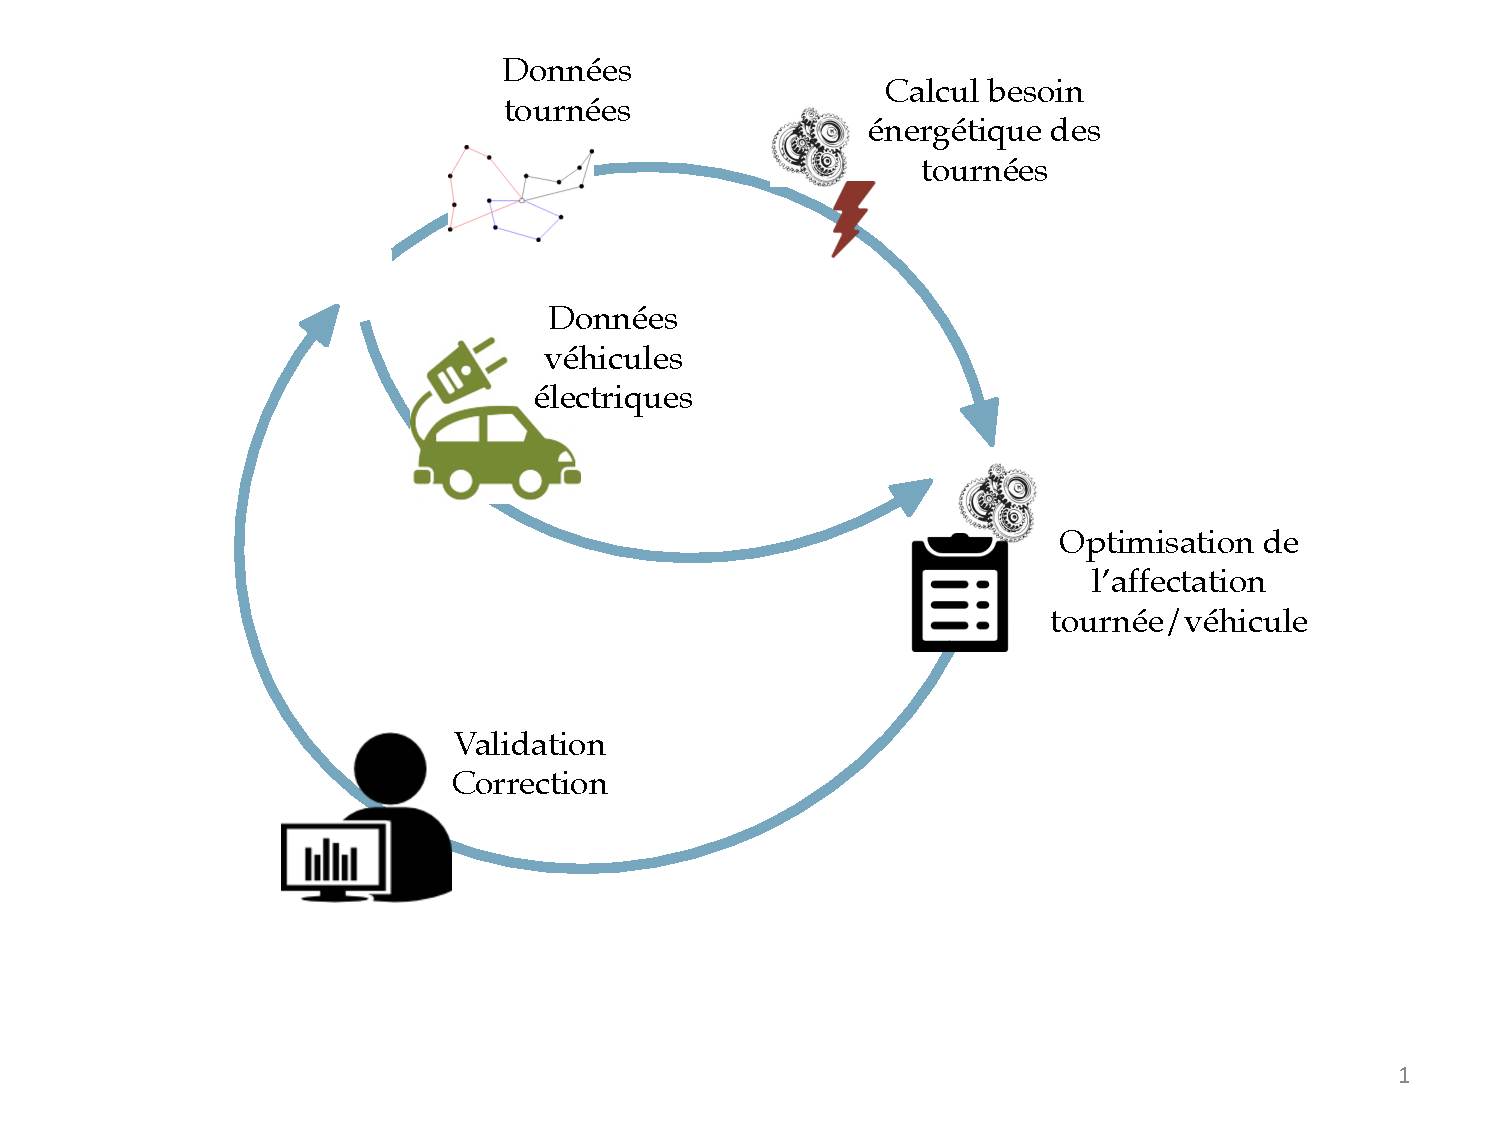
\includegraphics[trim=0cm 3cm 0cm 0cm, width=0.8\textwidth]{figures/5_implementation/processus_metier.pdf}
     \end{center}
     \caption{Processus d'affectation de véhicules électriques à des tournées}
     \label{fig:processus_metier}
    \end{figure}

    Pour ce cas d'étude, l'analyse de la structure exploite les liens de la vue
    intégration et la conformité du modèles d'architecture au métamodèle EA2M.
    L'analyse du comportement consiste à simuler l'ensemble de l'architecture en
    pilotant la simulation par le processus métier. Cette simulation a pour
    objectif de valider et critiquer  les choix de modélisation et d'anticiper
    l'éventuel dimensionnement de la flotte. Par exemple, si une forte
    proportion des tournées implique une distance effectuée supérieure à
    l'autonomie des véhicules électriques sans possibilité de recharge en cours
    de route (pas de borne à disposition au cours de la tournée), la simulation
    permet  de trouver la proportion de véhicules thermiques à garder a minima
    dans une flotte. L'affectation doit aussi privilégier l'utilisation des
    véhicules électriques car la rentabilité d'un parc de véhicules électriques
    est proportionnelle au nombre de kilomètres effectués par ces véhicules.

    \subsection{Mise en œuvre du \emph{framework ExecuteEA}\\
    pour la modélisation des vues métier, fonctionnelle et applicative}

    La première étape consiste donc à créer les modèles des vues métier, fonctionnelle
    et applicative en recourant à des langages de modélisation exécutables. Selon les
    propositions de ces travaux de thèse, l'usage de ces langages automatisent
    la manipulation des modèles et facilitent leur analyse. La
    figure~\ref{fig:architecture_generale_usecase} présente l'architecture \emph{in globo}
    du cas métier ainsi modélisé, selon le cadre structurant \emph{ExecuteEA}.






% Nous éprouvons notre démarche au cas métier de la gestion d'une flotte de
% véhicules électriques. Nous construisons les modèles adéquats pour les vues
% métier, fonctionnelle et applicative en adoptant des langages exécutables. La
% cohérence est modélisée dans la vue intégration. L'architecture globale du cas
% métier est illustrée dans la \ref{fig:architecture_generale_usecase}.


\begin{figure}[!htbp]
 \begin{center}
  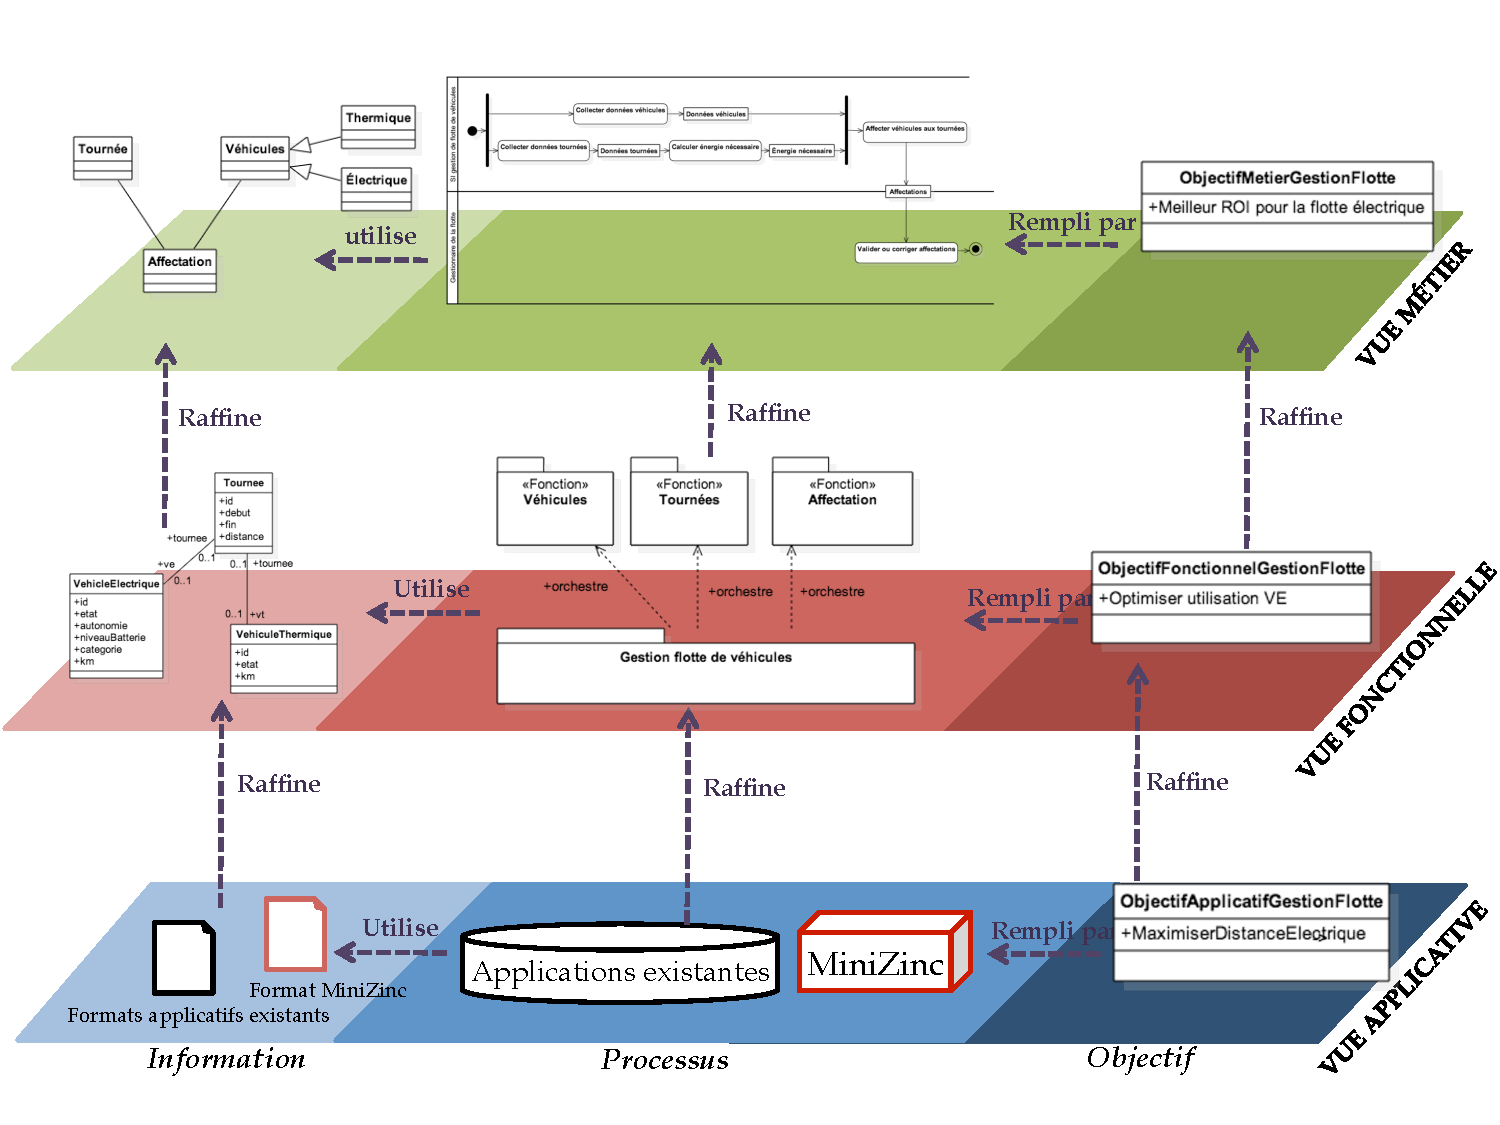
\includegraphics[angle=90, width=1\textwidth]{figures/5_implementation/architecture_generale_usecase.pdf}
 \end{center}
 \caption{Architecture globale du cas d'étude \\mettant en œuvre le \protect\emph{framework ExecuteEA}}
 \label{fig:architecture_generale_usecase}
\end{figure}


\subsubsection{Modélisation de la vue métier} 

Nous utilisons fUML comme langage
exécutable pour modéliser cette vue. Le processus métier consiste à collecter
les données relatives aux véhicules (électriques et thermiques) ainsi qu'aux
tournées à effectuer, de calculer l'énergie nécessaire à chaque tournée et
l'affectation véhicule/tournée avant de faire valider cette dernière par le
manager de flotte. Nous modélisons ce processus métier sous forme de diagramme
d'activité fUML en utilisant l'atelier de modélisation Papyrus. Selon notre cadre
d'architecture, les modèles créés représentent donc l'aspect processus de la vue
métier. La figure~\ref{fig:processus_fuml} présente le diagramme d'activité fUML obtenu à
l'aide de Papyrus.

\begin{figure}[!htbp]
 \begin{center}
  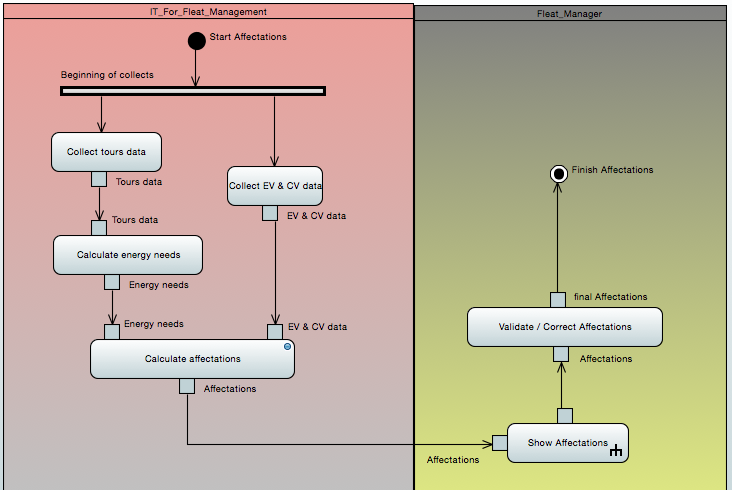
\includegraphics[width=1\textwidth]{figures/5_implementation/processus_fuml.png}
 \end{center}
 \caption{Aspect processus de la vue métier modélisé sous la forme d'un diagramme d'activité fUML avec Papyrus}
 \label{fig:processus_fuml}
\end{figure}


Pour l'aspect information, nous utilisons des diagrammes de classe UML pour
représenter les concepts métier et leurs relations. Nous modélisons ainsi les
concepts de Véhicule, Tournée et Affectation. La figure~\ref{fig:information_metier}
présente le diagramme de classes fUML modélisé dans Papyrus.

\begin{figure}[!htbp]
 \begin{center}
  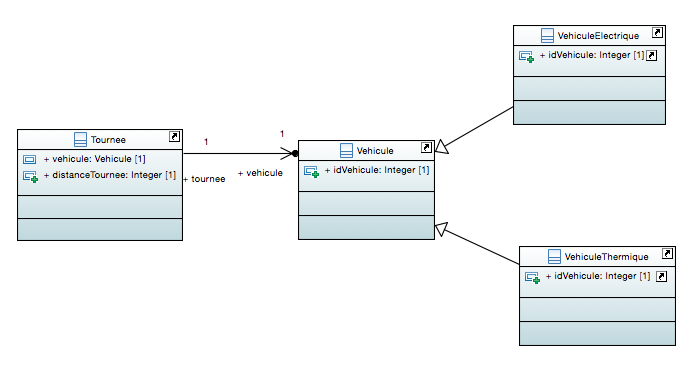
\includegraphics[width=1\textwidth]{figures/5_implementation/information_metier.png}
 \end{center}
 \caption{Aspect information de la vue métier modélisé sous la forme d'un diagramme de classes fUML avec Papyrus}
 \label{fig:information_metier}
\end{figure}

Gérer une flotte de véhicules peut
avoir plusieurs objectifs métier. Dans notre cas, obtenir le meilleur retour sur
investissement suite à l'intégration de véhicules électriques dans la flotte de
véhicules. Nous modélisons l'objectif métier sous la forme d'une classe UML
représentant l'aspect objectif de la vue métier comme l'illustre la 
figure~\ref{fig:architecture_generale_usecase}.

% Le choix des langages de modélisation et de l'outil de simulation est motivé par
% les pratiques du domaine. En effet, la Commission Électrique Internationale a
% adopté Enterprise Architect comme outil pour maintenir et distribuer le
% CIM\footnote{Common Information Model}\cite{uslar2012standardization}, un modèle
% d'information commun pour le domaine électrique
% \footnote{www.sparxsystems.com.au/press/articles/iec.html}.
	

\subsubsection{Modélisation de la vue fonctionnelle}

Nous modélisons l'aspect information de la vue fonctionnelle sous la forme d'un diagramme de classes
fUML. Ce modèle raffine les concepts métier en spécifiant leurs types. Dans la
vue fonctionnelle, le concept d'allocation prend la forme d'une association
entre les véhicules et les tournées. 

\begin{figure}[!htbp]
 \begin{center}
  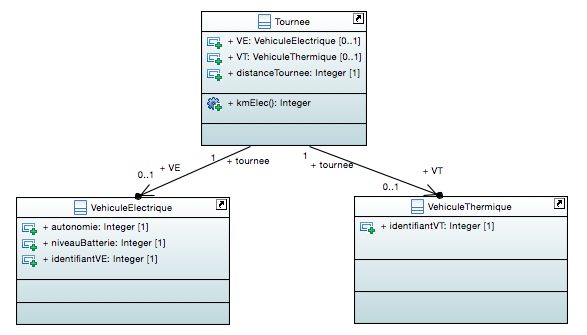
\includegraphics[width=1\textwidth]{figures/5_implementation/information_fonctionnelle.png}
 \end{center}
 \caption{Aspect information de la vue fonctionnelle modélisé sous la forme d'un diagramme de classes fUML avec Papyrus}
 \label{fig:information_fonctionnelle}
\end{figure}

L'objectif fonctionnel est d'optimiser
l'utilisation des véhicules électriques pour atteindre l'objectif métier qui est
d'avoir un meilleur retour sur investissement. Nous modélisons cet objectif 
sous la forme d'une classe UML
représentant l'aspect objectif de la vue fonctionnelle comme l'illustre la 
figure~\ref{fig:architecture_generale_usecase}.

Pour l'aspect processus de la vue fonctionnelle, nous commençons par identifier trois blocs fonctionnels~:
un bloc pour la gestion de la flotte de véhicules (électriques et thermiques),
un bloc pour la gestion des tournées, un bloc pour la gestion de l'affectation
(voir figure \ref{fig:architecture_generale_usecase}. Ces blocs contiennent les
fonctions qui raffinent les tâches du processus métier. Comme expliqué plus tôt
dans la démarche, le fait de les rassembler dans des blocs selon les concepts
métier augmente la modularité et l'évoluvilité de l'architecture. De plus, nous
consacrons un bloc à la gestion des processus fonctionnels. Ce bloc est
responsable de l'orchestration des fonctions du processus fonctionnel.

Les blocs fonctionnels offrent une vue plus détaillée des tâches métier. 
Pour ce cas d'étude, nous détaillons uniquement la tâche métier qui consiste à
affecter un véhicule à une tournée. Nous modélisons l'affectation des véhicules 
aux tournées
sous la forme de contraintes \gls{ocl}~: pour affecter un véhicule à une tournée, il
faut que l'énergie nécessaire à celle-ci soit inférieure à l'autonomie de la
batterie. Dans notre cas d'application, nous considérons qu'il n'est pas
possible de recharge le véhicule pendant la tournée de l'agent.

Nous modélisons la fonction d'affectation sous la
forme de deux contraintes et d'une requête en utilisant OCL. La première contrainte OCL signifie
que si un véhicule électrique est affecté à une tournée alors l'énergie dont il
dispose permet d'assurer la totalité de la tournée. La deuxième contrainte
signifie que si aucun véhicule électrique n'est capable d'assurer une tournée
donnée alors c'est un véhicule thermique qui lui est associé. Enfin, la requête
calcule le nombre total de kilomètres électriques correspondant à la distance
parcourue par les véhicules électrique après l'affectation. Cette requête permet
d'évaluer l'utilisation  des véhicules électriques dans l'optique d'atteindre
l'objectif fonctionnel.

Il est possible de modéliser les autres algorithmes de
traitement (calcul des tournées à partir de bon de travaux, calcul de l'énergie
nécessaire à une tournée, etc.) à l'aide de diagrammes d'activité exécutables.



\lstinputlisting[caption=Contraintes OCL pour la fonction d'affectation]{figures/5_implementation/tournee.ocl}

\subsubsection{Modélisation de la vue applicative}

Pour les processus applicatifs, nous commençons par identifier  les applications
nécessaires à l'implantation des blocs fonctionnels. Dans notre cas, le
patrimoine applicatif de l'entreprise dispose déjà d'applications pour la
gestion de tournées (calcul de tournées optimisé à partir de bons de travaux) et
la gestion de véhicules (administration, maintenance, etc.). Pour la fonction
d'allocation, nous faisons le choix d'utiliser MiniZinc pour modéliser les
contraintes au niveau applicatif \ref{fig:contraintesMiniZinc}.

\begin{figure}[!htbp]
 \begin{center}
  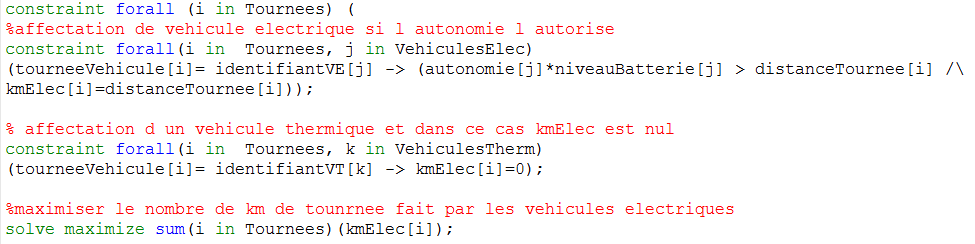
\includegraphics[width=1\textwidth]{figures/5_implementation/module_minizinc.png}
 \end{center}
 \caption{Contraintes du module MiniZinc}
 \label{fig:contraintesMiniZinc}
\end{figure} 

MiniZinc est un langage de modélisation et de résolution de contraintes de
niveau intermédiaire qui a pour vocation de devenir un langage de modélisation
standard dans le domaine de la programmation par contraintes. L'aspect
information contient les formats de données nécessaires aux différentes
applications. La figure \ref{fig:formatMiniZinc} représente le fichier de
données (le format .dzn) nécessaire à l'application MiniZinc pour calculer
l'affectation.

\begin{figure}[!htbp]
 \begin{center}
  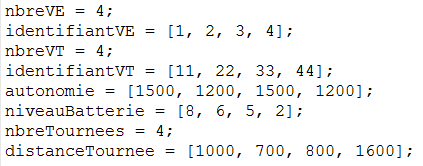
\includegraphics[width=0.5\textwidth]{figures/5_implementation/format_minizinc.png}
 \end{center}
 \caption{Fichier de données pour le module MiniZinc}
 \label{fig:formatMiniZinc}
\end{figure} 

Nous modélisons l'objectif applicatif sous la forme d'une classe UML
représentant l'aspect objectif de la vue applicative comme l'illustre la
figure~\ref{fig:architecture_generale_usecase}. Un véhicule électrique devient
rentable par rapport à un véhicule thermique à partir d'un certain nombre de
kilomètre parcouru. C'est pourquoi l'objectif fonctionnel qui est d'optimiser
l'usage de la flotte électrique se traduit par la maximisation du nombre de
kilomètres électriques, c'est à dire affecter aussi souvent que possible un
véhicule électrique aux tournées. Ainsi, le module MiniZinc prend en compte cet
objectif en résolvant les contraintes tout en maximisant la distance électrique.



\subsection{Intégration et analyse de la structure}

L'approche conceptuelle que nous proposons pour le \emph{framework ExecuteEA},
illustrée par la figure~\ref{fig:approche_conceptuelle} à la
page~\pageref{fig:approche_conceptuelle}, met l'accent sur le rôle intégrateur
de l'architecte d'entreprise~: il doit s'assurer de la cohérence intra-vue et
inter-vues de l'architecture globale tout en collaborant avec les architectes
métier, fonctionnel et applicatif.

L'intégration de l'architecture passe par la modélisation de la vue intégration,
c'est-à-dire par la spécification des liens de cohérence  intra-vue et et inter-
vues conformément au métamodèle EA2M. Nous avons donc modélisé ces liens pour
l'ensemble des vues métier, fonctionnelle et applicative. Néanmoins, la figure
\ref{fig:integration_gestion_flotte} ne présente qu'une partie modèles
d'intégration pour des raisons de lisibilité. Nous y modélisons à titre
d'illustration les liens de cohérence intra-vue entre la fonction d'affection,
ses inputs et output en termes de types fonctionnels, ainsi que son objectif
fonctionnel. Nous faisons de même pour le module d'optimisation MiniZinc, ses
inputs et outputs ainsi que l'objectif applicatif qu'il remplit. Le même
principe d'intégration intra-vue, c'est à dire entre les aspects d'une même vue,
est applicable à tous les autres éléments de la vue métier, fonctionnelle et
applicative.

\begin{figure}[!htbp]
 \begin{center}
  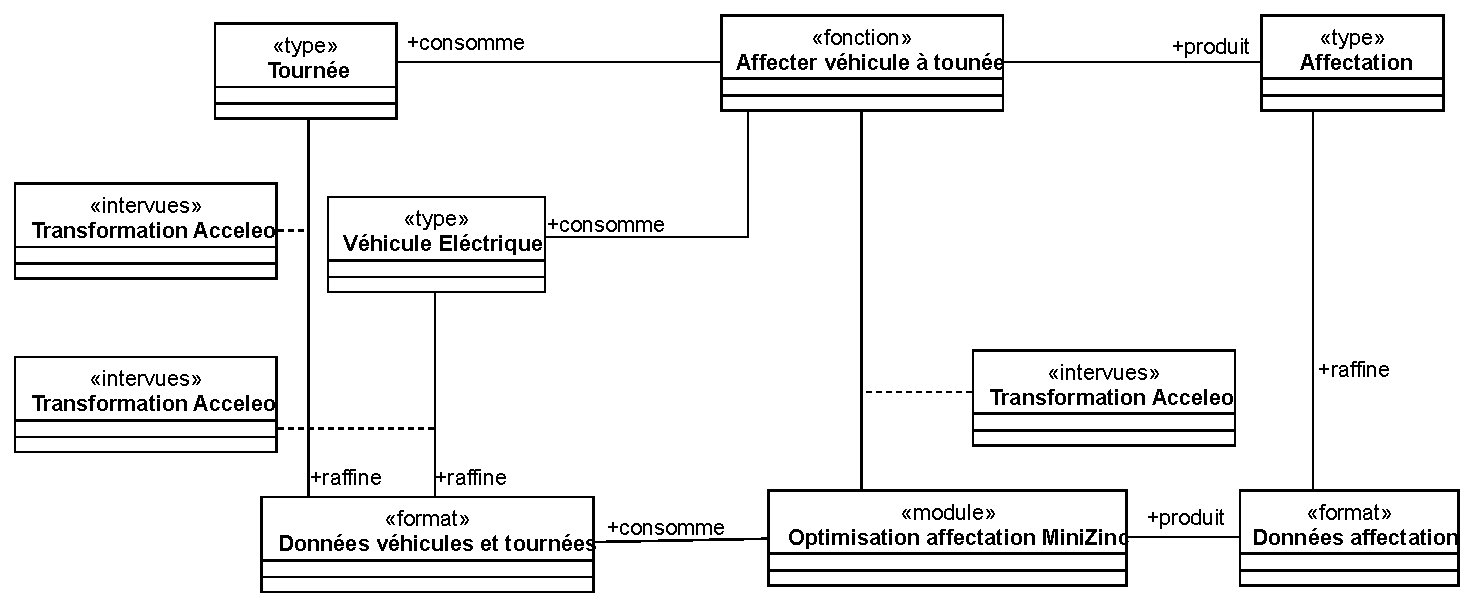
\includegraphics[trim= 0cm 0cm 0cm 0cm, width=1\textwidth]{figures/5_implementation/integration_affectation.pdf}
 \end{center}
 \caption{Une vue partielle des modèles d'intégration \\de la vue fonctionnelle et de la vue applicative}
 \label{fig:integration_gestion_flotte}
\end{figure}

De la même manière, nous modélisons les liens de cohérence inter-vues. Par
exemple, le lien \q{consomme} exprime qu'un type de données est compatible avec
la fonction qui l'utilise et qu'un format est compatible avec le module
applicatif qui l'utilise en entrée. Pour garantir une bonne orchestration des
processus, il faut que le \q{produit} d'une tâche (respectivement une fonction,
un module applicatif) soit compatible avec le ce que produit la tâche suivante
(respectivement une fonction, un module applicatif).

L'intégration passe aussi par l'identification des éventuelles transformation de
modèles. Rappelons ici que les transformations ont pour objectif d'améliorer
l'alignement métier/IT en automatisant le passage d'une vue à une autre. Pour le
cas métier de la gestion de flotte de véhicules, nous utilisons une
transformation de modèle pour générer les contraintes pour le module de calcul
d'affectation MiniZinc de la vue applicative à partir des contraintes OCL
exprimées dans la fonction affectation de la vue fonctionnelle. La
transformation est écrite dans le langage de transformation Acceleo. En plus de
transformer les contraintes décrite dans l'aspect métier, cette transformation
de modèle permet aussi de transformer les instances des types fonctionnels en
instances dans le format \q{.dzn} utilisé par le module MiniZinc comme
l'illustre la figure \ref{fig:integration_gestion_flotte}. La génération de code
pour le module MiniZinc peut être lancée à partir de la vue fonctionnelle que
nous avons précédemment modélisée dans Papyrus comme l'illustre la
figure~\ref{fig:acceleo_papyrus}.

\begin{figure}[!htbp]
 \begin{center}
  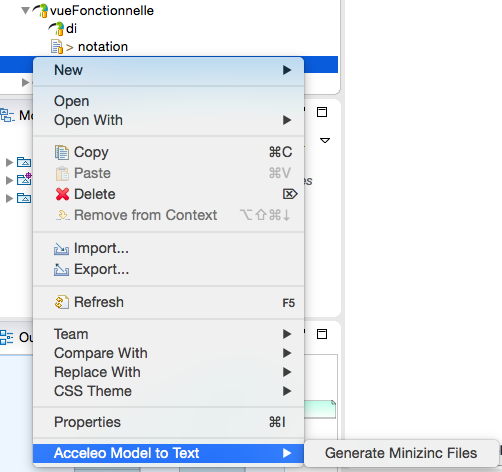
\includegraphics[width=0.7\textwidth]{figures/5_implementation/acceleo_papyrus.png}
 \end{center}
 \caption{Génération du code pour le module MiniZinc\\à partir de la vue fonctionnelle dans Papyrus}
 \label{fig:acceleo_papyrus}
\end{figure}


\subsection{Simulation et analyse du comportement}

Grâce aux langages exécutables, l'analyse du comportement des modèles
d'architecture se fait directement dans les langages de modélisation utilisés
pour les vues. Avec le \emph{framework} ExecuteEA, nous proposons de simuler de
l'ensemble de l'architecture en la pilotant par l'exécution du processus métier.
La simulation du processus métier se traduit par l'exécution du diagramme
d'activité fUML à l'aide du moteur d'exécution Moka intégré à Papyrus. Un des
avantages de l'outil Papyrus est de permettre la modélisation \emph{et} la
simulation de l'architecture dans un même environnement.

Notre approche préconise de modéliser les détails des taches dans les vues
inférieure afin de respecter le niveau d'abstraction requis par chaque point de
vue et ainsi de ne pas altérer la compréhension des parties prenantes de la vue
qui leur destinée. Par exemple, l'analyse métier n'aura ainsi pas à discuter du
détails des applications implémentant les tâches métier avec l'architecte
applicatif.

Comme expliqué dans la section~\ref{sec:opaque_action_papyrus}, Papyrus offre la
possibilité d'étendre la sémantique d'exécution de fUML à travers les
\emph{Opaque Action}. Celles-ci permettent d'invoquer des modules d'applications
extérieures au moment de l'exécution du diagramme d'activité fUML.
Développée pour les besoins du cas d'étude, cette extension rend possible l'invocation directe
du module MiniZinc pendant l’exécution du processus métier pour optimiser
l'affectation des véhicules aux tournées. Rappelons que le module MiniZinc est
obtenu par transformation de modèle à partir de la vue fonctionnelle.

La simulation prend la forme d'une animation de diagramme. La figure
\ref{fig:simu_capture_ecran} est une capture d'écran montrant la simulation du processus métier
en cours d'exécution. Papyrus offre la possibilité de mettre des \emph{breakpoints} sur
certaines activités et de paramétrer le pas de temps pour contrôler le
déroulement du processus.

\begin{figure}[!htbp]
 \begin{center}
  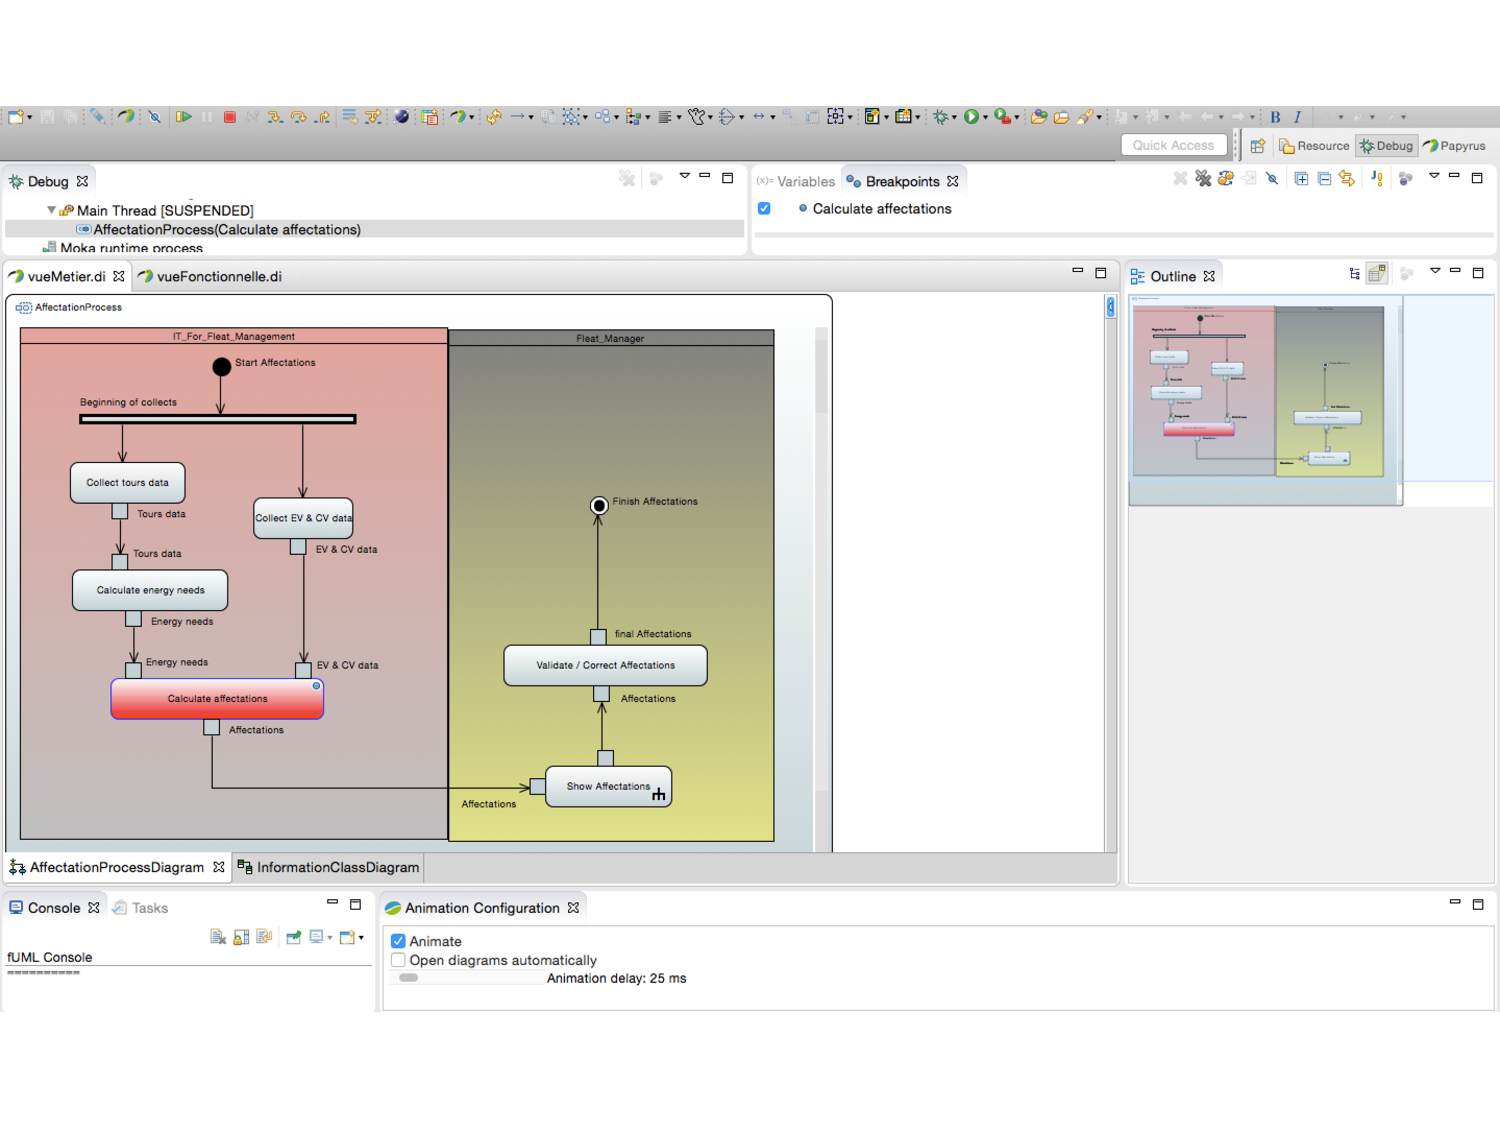
\includegraphics[angle=90, width=1\textwidth]{figures/5_implementation/simu_capture_ecran.pdf}
 \end{center}
 \caption{Simulation de l'architecture sous Papyrus}
 \label{fig:simu_capture_ecran}
\end{figure}

La simulation retourne comme résultat les affectations des véhicules aux
tournées. Ce résultat est affiché dans la console fUML comme l'illustre la
figure \ref{fig:resultat_simu}. La simulation a pour objectif de voir si
l'utilisation des véhicules électrique est rentable en comparant la distance
parcourue par le véhicule électrique et la distance minimale permettant de le
rentabiliser. Dans ce cas, il est par exemple envisageable de reconfigurer les
tournées de manière à ce que plus de véhicules électriques soient affectés. En
effet, notre démarche a pour but l'analyse fonctionnelle. La validation s'appuie
sur les indicateurs dérivés de l'aspect objectif et sur l'avis des experts. Des
analyses statistiques peuvent être conduites mais elles ne rentrent pas dans le
périmètre de nos travaux.

\begin{figure}[!htbp]
 \begin{center}
  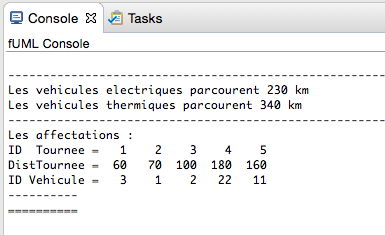
\includegraphics[width=0.6\textwidth]{figures/5_implementation/resultat_simu.png}
 \end{center}
 \caption{Résultat retourné par la simulation du cas d'étude dans Papyrus}
 \label{fig:resultat_simu}
\end{figure} 

Comme exposé dans l'état de l'art, l'approche ExecuteEA s'inscrit dans l'école
de pensée \emph{Enterprise System Architecting}~: par l'analyse du comportement
de l'architecture, nous souhaitons non seulement vérifier l'alignement de l'IT à
la stratégie de l'entreprise mais aussi donner la possibilité au métier
d'évaluer sa propre stratégie en fonction de sa déclinaison au niveau de l'IT.
Dans le contexte de la gestion d'une flotte de véhicules électriques, la
simulation peut aboutir à la non adéquation du type de tournées avec l'impératif
de rentabiliser l'investissement dans une flotte de véhicules électriques à
cause de la distance des tournées. En pareil cas, les architectes —~métier,
fonctionnel et applicatif~— en étroite collaboration avec l'architecte
d'entreprise peuvent envisager de faire évoluer l'application qui optimise les tournées quotidiennes 
crées à partir des bons de travaux pour en écourter la distance.




%\section{analyse de la structure}
%Validate modèle -> pour tester l'intégrité du modèle
%Requêtes sur le modèle OCL
%Si appli hirs service quel sont les processus impacté etc.
%Un nouveau process faisant intervenir d'ancienne tâche, quelle ancienne appli réutilisée
%Détecter les problèmes d'interop' entre modules
 
%\lstinputlisting{figures/5_implementation/affectations.mzn}

\section[Discussion et perspectives]{Discussion et perspectives pour le prototypage\\
            et la validation du \emph{framework} ExecuteEA}

    Le développement du prototype et son application au cas métier
    de la gestion d'une flotte de véhicules électriques concrétise l'ensemble des
    propositions autour du \emph{framework} ExecuteEA et du métamodèle EA2M
    et fournit un outil d'analyse de la structure et du comportement
    d'une architecture d'entreprise.

    Bien que nous n'avons modélisé et simulé qu'un seul processus métier, la mise
    en œuvre du \emph{framework} ExecuteEA a permis de valider les apports de l'IDM
    en tant que cadre technologique et méthodologique aux différentes activités d'EA.
    La première limite de cet implémentation est donc le passage à l'échelle. C'est en effet dans le
    traitement d'une grande quantité d'artefacts utiles à l'EA, dont la gestion dépend souvent du 
    savoir-faire de l'architecte d'entreprise uniquement
    sans assistance informatique particulière, que notre  proche prouve sa valeur.

    Une premier passage à l'échelle serait donc de d'élargir le cas métier en incluant par exemple
    le processus de calcul de tournées journalières à partir de bons de travaux, le processus
    de recharge de la batterie et ses impacts sur le réseau électrique, le processus d'entretien des
    voitures, le processus de réservation de voitures par d'autres agents non impliqués dans les tournées,
    etc. 

    Lors de la simulation du processus métier, nous avons implémenté la
    tâche de l'affectation de véhicules aux tournées. Cette implémentation a consisté à modéliser
    la fonction qui réalise cette tâche sous la forme de contraintes OCL puis à obtenir par transformation
    de modèle le code pour le module MiniZinc de la vue applicative. 
    Ces développements valident le principe
    de simulation que nous proposons (cf. figure~\ref{fig:Simulation_Approche} page~\pageref{fig:Simulation_Approche}).
    Il serait donc intéressant de l'étende au reste des tâches métier du processus en utilisant cette fois des diagrammes
    d'activité fUML pour modéliser et simuler leur comportement.

    De manière générale, bien qu'il ne s'agisse que d'un prototype, l'implémentation de la vue intégration avec EMF
    a permis de mettre en lumière les avantages que présente la méta-modélisation pour l'analyse structurelle
    des modèles d'architecture, notamment grâce à la relation de conformité qui lie un modèle à son métamodèle.
    La méta-modélisation avec Ecore est d'autant plus pertinente avec le recours aux contraintes OCLinEcore
    permettant de préciser d'avantage le métamodèle EA2M. Ces mêmes contraintes peuvent aussi servir à
    exprimer des requêtes sur le modèles. À titre d'exemple, nous sommes en train de développer des requêtes
    permettant de retrouver toutes les tâches (respectivement
    fonctions et modules) utilisant un certain concept (respectivement type et format). Une multitude de requêtes de ce
    type gagnent à être développées pour faciliter l'analyse structurelle de l'architecture.

    Enfin, la question de l'adoption des langages de modélisation par les différents parties-prenantes (architectes
    d'entreprise, métier, fonctionnel, applicatif) est cruciale. Bien que l'utilisation de UML comme
    langage de modélisation n'est pas évident de prime abord par des personnes à profile non technique,
    les spécifications des use case Smart Grids recourent de plus en plus à UML au sein de la \gls{cei}.
    Les entretiens menés avec les différents experts d'EA et du réseau électrique révèlent cependant la frilosité
    de certaines personne à adopter UML pour décrire leurs spécifications dans leur intégralité. Néanmoins, ces
    personnes recourent de plus en plus à certains diagrammes comme les diagrammes d'activités pour décrire
    leurs processus. Dans ce contexte, le choix de fUML et de OCL nous semble être \q{raisonnable}.  

    % De manière nous avons mis l'accent sur la simulation est pas assez sur l'analyse de la structure. 


	\chapter{Méthodologie de la recherche}
\label{ch:methodo}

La méthodologie de recherche permet non seulement de comprendre la mise en place 
d'une démarche de recherche mais aussi les résultats l'étude. Le but de ce 
chapitre est double. D'une part, nous veillons à démonter l'adéquation entre 
notre démarche et l'objet de recherche. D'autres part, ce chapitre éclaire le 
cheminement des travaux de recherche pour comprendre la construction de la 
démarche adoptée. 

Une démarche classique de recherche commence par la formulation d'une question 
de départ. La question qui a initié nos travaux est la suivante~: «~Comment 
simuler afin de les valider les SI des Smart Grids ?~».  Comme en témoigne notre 
l'état de l'art, cette question fait l'objet de très peu de travaux (section 
\ref{approche_simu_existante}). Une recherche exploratoire a donc été nécessaire 
pour mettre en évidence les caractéristiques d'un phénomène nouveau selon une 
démarche inductive. 

Cette phase exploratoire a été préalable à la définition du cadre d'architecture 
\textit{ExcuteEA}. La construction de ce cadre d'architecture et sa mise à 
l'épreuve ont fait l'objet d'une recherche explicative pour laquelle nos avons 
adopté une démarche déductive.

L'intérêt de cette partie est de traiter la question de la cohérence entre nos 
objectifs de recherche et la démarche que nous adoptons pour y répondre. Mais 
nous ne cherchons pas à donner l'impression que notre plan de recherche a été 
entièrement établi avant de le mettre en œuvre. À l'inverse, nous l'avons 
construit au fur et à mesure de nos interactions avec le terrain d'étude. 

Tout d'abord, nous présentons la démarche inductive entreprise pour délimiter 
notre objet d'étude. Nous reprenons les étapes de cette recherche exploratoire 
par ordre chronologique~: exploration de la vue métier, puis de la vue 
applicative et en fin de la vue fonctionnelle. Nous présentons ensuite la 
démarche déductive ayant abouti à la construction du cadre d'architecture 
ExecuteEA.

%"Quelle que soit la nature de la démarche, la capacité d'ouverture et de prise 
%en compte d'éléments nouveaux est primordiale." ici ou dans la conclusion ?

%Dans une démarche classique de recherche, la définition de l'objet d'étude est 
%préalable à la 
%Plusieurs méthodes de recherche
%démarches de recherches employée par ordres chronologiques
%Combinaisons de méthodes 
%Vocation exploratoires de nos recherches
%Nous ne cherchons pas ici à donner l'impression que nous avons entièrement mis 
%au point notre plan de recherche avant de le mettre en œuvre. Celui-ci s'est au 
%contraire construit au fur et à mesure de notre interaction avec le terrain.
%
%"la cohérence du protocole de recherche avec la nature des questions que nous 
%nous posons"
%"Mais un autre élément mérite d'être distingué : la délimitation de l'objet 
%d'étude pose des problèmes tels qu'elle constitue une recherche en elle-même"
%"Quelle que soit la nature de la démarche, la capacité d'ouverture et de prise 
%en compte d'éléments nouveaux est primordiale."


	\section{Délimitation de l'objet de recherche}
%	Q : Est-ce que le recours à la demarche inductive est bien justifié ?
%		Est-ce l'investigation satisfait bien les critères de cohérence interne ?
		
	Une attention singulière est apportée à la délimitation de l'objet d'étude. 
Cette délimitation est souvent le résultat de l'observation du terrain d'étude~: 
l'entreprise et son SI d'une manière générale et l'entreprise et son SI dans le 
cas particulier des Smart Grids. L'entreprise et son SI forment un système 
complexe dont l'observation n'est pas triviale. La délimitation de l'objet 
d'étude a donc été en soi à l'origine d'une démarche de recherche.
	
	Cette partie a pour objectif de démonter la pertinence d'une démarche inductive 
pour l'identification de notre objet d'étude. D'une part, une démarche inductive 
est utile pour formuler des hypothèses ou soulever des questions et pour aborder 
un problème qui a été peu étudié comme c'est le cas de la simulation des SI. 
Elle aboutit à des propositions générales à partir de cas particuliers~: c'est 
une démarche par exploration. 
	Cette démarche est donc adaptée pour~: 
	\begin{enumerate}
	\item délimiter l'objet de l'étude, c'est à dire identifié ce qui est dans le 
contexte de la simulation des SI et ce qui ne l'est pas~;
	\item jeter les bases d'une étude théorique ultérieure.
	\end{enumerate}
	
	D'autre part, l'induction est une démarche de recherche classique en sciences 
sociales. Elle correspond au raisonnement empiriste qui affirme que 
l'observation et l'expérience sont la source de la connaissance du monde réel et 
du concret \cite{madeleine2001methodes}. Nous cherchons en effet à comprendre 
notre objet d'étude empiriquement. Le recours à cette démarche est d'autant plus 
justifié par la nature socio-technique du SI. En définissant le SI, Robert Reix 
met en évidence sa composante sociale (\ref{ch:EA}). 
	
	%Une étude ethnographique est Notre démarche inductive est donc doublée d'.

	La volonté d'identification de notre objet d'étude est portée par la question 
suivante «~Qu'est ce que la simulation d'un SI d'entreprise ?~». Néanmoins, même 
empirique, une démarche de recherche doit nécessairement s'inscrire dans un 
cadre de cohérence. Nous avons donc veillé à construire un protocole 
d'investigation épistémologiquement valide et conforme aux critères de cohérence 
interne. Notre protocole d'investigation est axé sur l'observation et 
l'expérience. Il est constitué de trois grandes étapes ~:
		
		\begin{enumerate}
		
	\item observation du terrain d'étude, c'est à dire analyse des pratiques 
courantes des personnes concernées par la simulation. Nous avons identifié deux 
catégories de personnes susceptibles de nous intéresser~: les experts (en SI ou 
en simulation) et les personnes susceptibles d'instrumenter la simulation des SI 
pour leurs travaux de recherche ou d'ingénierie (il s'agit là des utilisateurs 
finaux). Nous avons privilégié les ingénieurs-chercheurs d'\gls{edf}~R\&D car le 
contexte \gls{cifre} de la thèse a facilité l'accès à ces 
personnes.L'observation aboutit à la formulation d'hypothèses «~aprioristes~». 
Ce type d'hypothèse est exploratoire car elles ont pour but de soulever des 
interrogations~;
	%observatio participative, démarche ethnographique
	
	\item développement d'un prototype de simulation tenant compte du résultat des 
observations de l'étape précédente. Le prototype n'a pas pour vocation de 
proposer une solution finale mais plutôt tester rapidement les hypothèses 
formulées précédemment~;
	
	\item validation ou mise à l'épreuve du prototype sur le terrain d'étude. Cette 
mise à l'épreuve commence par la définition d'un cas d'application pertinent 
permettant de vérifier les hypothèses formulées à l'étape d'observation. Elle se 
poursuit par la collecte et l'analyse du retour des personnes concernées. Le 
contexte \gls{cifre} a là aussi facilité les échanges avec les 
ingénieurs-chercheurs de EDF R\&D, et en particulier ceux du département 
\gls{mire}. Notre intégration à l'équipe des ingénieurs-cherches du département 
\gls{mire}, et en particulier à l'équipe du projet de simulation des Smart Grid, 
a contribué à la qualité des échanges avec les personnes interrogées.
	
		\end{enumerate}
		
	Le raisonnement par induction aboutit à des propositions générales à partir de 
cas singuliers. Nous avons donc commencer par décomposer le terrain d'étude, 
c'est à dire le SI de l'entreprise. Les bases théoriques de la discipline des SI 
ont permis de procéder à cette décomposition afin de mettre en évidence ses 
singularités. Les approches par points de vue sont largement utilisée pour 
traiter la complexité des SI en le décomposant en plusieurs vues~: la vue 
métier, la vue fonctionnelle, la vue applicative, la vue technique. Chaque vue 
correspond à la perspective d'un groupe de personnes aux profils différents mais 
complémentaires. Les investigations ont été menées sur les trois premières vue — 
métier, fonctionnelle, applicative. La vue technique n'a pas été traitée~: le 
temps nécessaire aux expérimentations est incompatible avec les délais de cette 
thèse et son financement dans le cadre d'une \gls{cifre}.
	
	Le protocole d'investigation est alors appliqué à chacune des vues métier, 
fonctionnelle et applicative. L'objectif de la démarche engagée est de définir 
l'objet d'étude, en ayant comme question de départ «~Qu'est ce que la simulation 
d'un SI d'entreprise ?~». Cependant, nous avons veillé à garder une capacité 
d'ouverture aux idées nouvelles. Nous présentons
	
		\subsection{Investigations menées pour la vue métier}
			La première étape d'observation a débuté avec un stage de fin d'étude de six 
mois que nous avons effectué au sein du département \gls{mire}. L'objectif du 
stage a consisté à explorer le sujet «~Simulation du SI des Smart Grids~» afin 
de préparer un sujet de thèse. Il s'est donc accordé avec l'objectif des 
investigations menées pour la vue métier.
			
			\subsubsection{Observation}
				Pour cette première phase d'observation, des entretiens ont été menés avec 
des experts SI internes à l'entreprise et mais aussi externes à celle-ci lors 
d'un séminaire professionnel ayant pour thème la modélisation des SI \footnote{Model Driven Day, 21 novembre 2001, Paris 
Cœur Défense}. Des entretiens ont aussi été menés avec des ingénieurs-chercheurs 
du département \gls{mire} ayant participé à des démonstrateurs Smart Grids 
européens pour mettre en évidence les pratiques de spécification de la 
composante SI des Smart Grids. 

				Les hypothèses formulées à l'issue des ces observations sont les suivantes~:
				\begin{itemize}
					\item la simulation de SI est une discipline peu étudiée~;
					\item la simulation des processus métier est pertinente pour les SI des 
Smart Grids dans le mesure ou elle permet de valider les scénarios élaborés pour 
les démonstrateurs, mais aussi pour les SI tout court~;
					\item lors de cette simulation, il est nécessaire de maintenir une 
cohérence entre le processus et les données qu'il manipule~;
					%\item les langages de modélisation exécutables présentent des avantages pour la simulation des SI.
				\end{itemize}
		
			\subsubsection{Prototypage}
				Le prototypage a nécessité une étude des outils existants proposant de 
simuler des processus métier, ce qui a permis d'identifier les outils suivant~: 
Enterprise Architect, Bonita, Amuse et Rhapsody. Il a ensuite essentiellement à 
tester leur capacité de simulation selon une grille d'évaluation. Le critère de 
sélection principal a été la capacité de l'outil à exécuter des diagrammes 
d'activité UML. En effet, c'est dans ce langage que sont représentés les 
processus métier dans les documents de spécification des démonstrateurs Smart 
Grid. Le deuxième critère d'évaluation retenu a été la possibilité d'ajout de 
nouvelles fonctionnalités à l'outil. À l'issue de cette étude comparative, 
l'outil Enterprise Architect dans sa version 9.2 a été retenu. En effet, à 
l'époque de l'étude, EA était le seul à pouvoir animer des diagrammes d'activité 
et à offrir la possibilité d'ajout de fonctionnalité par le mécanisme de plugin. 
C'était en outre l'outil de modélisation UML de référence de l'équipe 
d'ingénieurs-chercheurs au sein de laquelle nous avons effectué ce stage.
				
				Cependant, dans sa version 9.2, l'outil n'assure pas la cohérence entre les 
objets métier (modélisés avec diagramme de classe) et le processus (modélisé 
avec un diagramme d'activité) au cours de la simulation. De plus, l'outil ne 
gère pas la persistance des résultats de la simulation. La mise en cohérence a 
donc nécessité le développement d'un plugin que nous avons baptisé DataSimu. 
DataSimu permet de (1)~créer un jeu de donnée en entrée de la simulation à 
partir des concepts métier en instanciant un diagramme de classe (2)~simuler le 
processus métier avec ce jeu de donnée (3)~récupérer le jeu de données en sortie 
de la simulation et les stocker dans une base de données. Nous avons mené 
l'implémentation de DataSimu en binôme avec un étudiant en troisième année 
d'école d'ingénieur. L'interface graphique de DataSimu est illustrée par la 
figure. L'annexe (ANNEXE) détaille l'architecture de DataSimu et présente un 
manuel d'utilisation. 
				
\begin{figure}[!ht]
 \begin{center}
  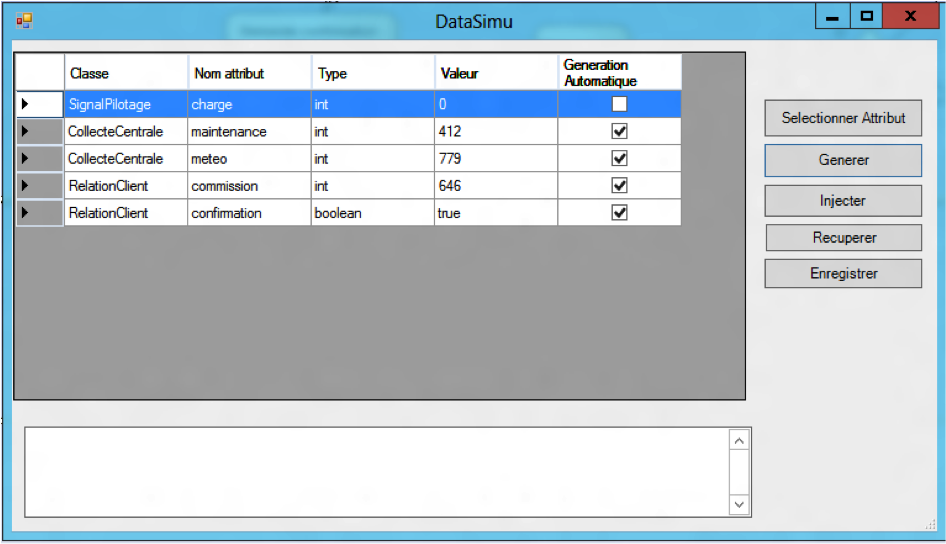
\includegraphics[width=1\textwidth]{figures/6_methodologie/data_simu.png}
 \end{center}
 \caption{Interface Graphique de DataSimu}
 \label{fig:data_simu}
\end{figure}
				
			\subsubsection{Validation}
			Pour valider les hypothèses formulées à l'issue de l'observation, un cas 
d'application Smart Grid a été mis au point~: le pilotage d'une charge 
domestique. Ce cas d'application est issu de l'étude des spécifications des 
démonstrateurs Smart Grid ADDRESS et PREMIO introduits dans la 
section~\ref{sec:DemonstrateursSG}. Il s'agit de piloter une batterie de 
stockage d'énergie installée chez un client (particulier ou industriel). En 
fonction de l'état du réseau, une centrale de pilotage contrôle cette batterie 
(stockage d'énergie pour une utilisation ultérieure), tout en tenant compte des 
consignes du client. Ce cas métier a été modélisé et simulé avec l'outil 
Enterprise Architect doté du plugin DataSimu. Une description détaillée du cas 
métier et du déroulement de la simulation est donnée dans l'annexe 
\ref{annexe:DataSimu}. 
			
			Le prototype de simulation et sa mise en œuvre à travers le cas métier du 
pilotage d'une charge domestique ont été soumis aux experts SI du département 
\gls{mire} et aux ingénieurs-chercheurs contribuant aux démonstrateurs Smart 
Grid PREMIO et ADDRESS. Les entretiens suivant la démonstration ont validé (1) 
la pertinence de la simulation dans le contexte des SI des Smart Grids (2) la 
séparation du processus métier et des objets métier tout en maintenant une 
cohérence lors de la simulation. 
			
			Ces entretiens, assortis l'étude des outils de simulation des processus 
métier, ont permis de constater que la question de la simulation est peu abordé 
dans le contexte des SI. Ces travaux d'investigation ont de plus donné lieu à 
une publication \cite{seghiri2012animation} et ont été poursuivis par les 
travaux présentés dans cette thèse.
 
				\subsubsection{Conclusion}
			Cette première itération du protocole d'investigation a conforté nos hypothèses initiales à savoir que la simulation est peu abordée dans le contexte des SI mais qu'elle est pertinente pour valider/critiquer les scénarios de cas métier Smart Grid avant leur implémentation.

			\subsection{Investigations menées pour la vue applicative} 
				La vue applicative tient une place de choix dans les SI des entreprises. Pour des SI fortement informatisé, il arrive même souvent que le SI soit réduit aux applications informatiques et à l'infrastructure qui les supportent. Cette constatation est encore plus avérée dans le cas des Smart Grids dont le principe est le déploiement de TIC sur le réseau électrique pour automatiser son pilotage. Le choix chronologique de poursuivre les investigations en abordant la vue métier découle de cette constatation.		
			
				\subsubsection{Observation}
				Les investigations menées pour la vue applicative ont nécessité d'approfondir nos connaissances du fonctionnement du réseau électrique. Pour cette deuxième phase d'observation, nous avons conduit des entretiens avec deux profiles de personnes~: des experts et des ingénieurs-chercheurs spécialisé dans le réseau électrique de distribution  appartement au département \gls{mire}. En effet, plus que les réseaux de transport, ce sont les réseaux de distribution qui sont concernée par les Smart Grids. Les réseaux de transports français sont déjà fortement automatisés. 
				L'objectif de ces entretiens est double~: approfondir nos connaissances du réseau électrique et comprendre les pratiques des personnes interrogées en matière de simulation.
				Les experts sus-mentionnés sont responsables de la conception d'applications pour la conduite du réseau électrique. Le langages de conception les plus utilisés sont les automates programmables. Les ingénieurs-chercheurs sont quand à eux responsable du développement des applications, le plus souvent en Matlab ou  C++.
				Les hypothèses formulées à l'issue de cette observation sont les suivante~:
				\begin{itemize}
					\item la simulation du SI pour les Smart Grid est liée à la simulation des réseaux électriques~;
					\item la simulation du SI des Smart Grid nécessite de traiter la problématique de l'hétérogénéité des modèles.
				\end{itemize}
				
				\subsubsection{Prototypage}
				Le cas d'application du pilotage d'une charge domestique n'a pas été utilisé pour le prototypage de la vue applicative. Les modèles de la vue applicative nécessitent un niveau de détail plus élevé que les modèles de la vue métier. Or les spécifications des démonstrateurs ADDRESS et PREMIO n'offrent pas le niveau de détails nécessaires. Le Use Case normalisé par \gls{enel} (voir section~\ref{sec:ENEL) pour la régulation de tension sur les réseau de distribution a été adopté et affiné par les discutions avec les ingénieurs-chercheurs du département \gls{mire} travaillant sur la même thématique. 
				Ils s'agit d'adapter la tension du réseau électrique en fonction de la charge et de la production pour maintenir un niveau de tension respectable. Les deux leviers d'action sont utilisés, les régleurs en charge et les \gls{der}. Les régleurs en charges pilotés à distance agissent sur le niveau de tension au niveau des postes sources. Le pilotage des \gls{der} permet de contrôler la quantité d'énergie qu'ils injectent sur le réseau. 
				
				Ce cas métier fait intervenir un SI qui calcule les consignes envoyées aux DER et au régleur en charge et un réseau électrique qui réagit à ces consignes. Nous avons utilisé l'outil Ptolemy\footnote{http://ptolemy.eecs.berkeley.edu/}de modélisation hétérogène pour développer un prototype de simulation. La figure~\ref{fig:simu_ptolemy} illustre le modèle de simulation. Les éléments modélisés sont le SI et le réseau électrique (\textit{Network}). Le comportement du SI est avec une machine à état.  
				
\begin{figure}[!ht]
 \begin{center}
  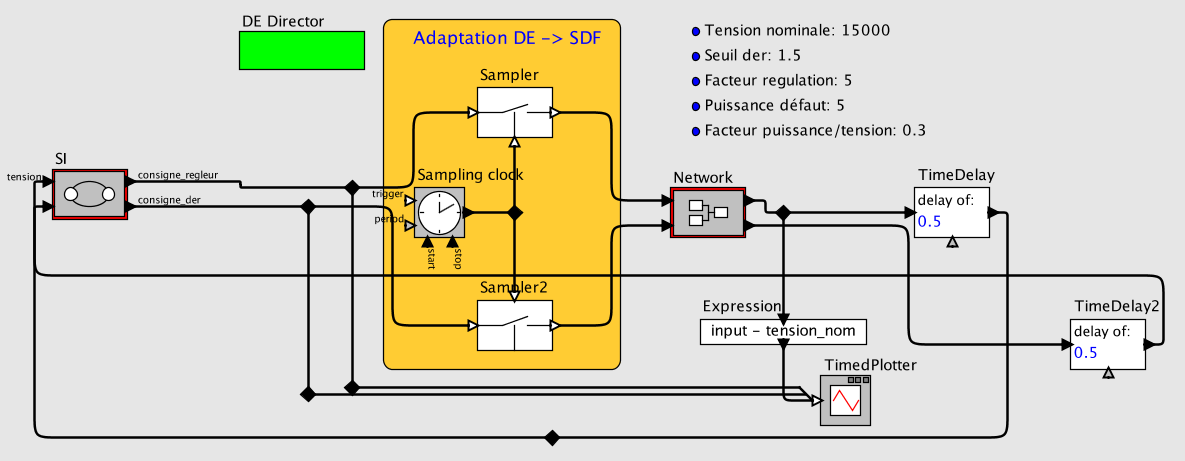
\includegraphics[trim = 0cm 5cm 0cm 0cm, width=1\textwidth]{figures/6_methodologie/simu_ptolemy.png}
 \end{center}
 \caption{Prototype Ptolemy pour une simulation hétérogène comprenant le SI (discret) et le réseau électrique (continue)}
 \label{fig:simu_ptolemy}
\end{figure}
		
				\subsubsection{Validation}
	Ptolemy : Simu appli + couplage réseau élec
			
	
		\subsection{Investigations menées pour la vue fonctionnelle} 
			\subsubsection{Observation}
		
			\subsubsection{Prototypage}
		
			\subsubsection{Validation}
	DSML pour le Volt Var Control
		
	
	
		\subsection{Conclusion}
Redéfinition de l'objet d'étude
Reformulation de la question de départ -> ref problématique 
Le cœur de la problématique 
Adéquation de la démarche et de l'objectif de la recherche (objet d'étude)
	
La question de l'analyse par simulation du SI fait l'objet de 
Démarche exploratoire / Démarche ethnographique 
La délimitation du sujet de recherches est en soit à l'origine d'une démarche de 
recherche à part entière  inductive, se prête mieux au sujet nouveau, faisant 
l'objet de peu de travaux
Jeter les bases d'une étude ultérieure


Mettre en évidence les caractéristiques du phénomène et construire des 
hypothèses 
"Les hypothèses et même les questions sont susceptibles d'évoluer au fur et à 
mesure de la recherche"

"En retour, le travail empirique se verra régulièrement réorienté en fonction 
des approfondissements successifs du cadre théorique "

Étude sociologique -> entretien avec les experts, sur leur avis de nos 
prototypes mais aussi 

Plusieurs démarches d'investigation 
prototypage et entretien 
ou SI transverse et SI spécialisé ? SI purement logiciel / SI socio-technique 
(interaction humaine) 
Une différence d'échelle 
		 


	\section{Conceptualisation / construction du cadre d'architecture 
\textit{ExecuteEA}}
%À partir de la compréhension empirique de notre objet d'étude et de la 
formulation d'une problématique 
La reformulation de la question de départ abouti à la définition d'une 
problématique 
La question de départ est au cœur de la problématique 

permet la Définition du cadre théorique 

La proposition est au contraire déductive
Sujet identifiés, hypothèses formulées
systèmes similaires : SI et entreprise -> établir les similarités
Les hypothèses etc.  
Choix de la théorie à appliquer : IDM (hypothèse et conclusion)/ apport de l'IDM 
a-à l'EA, hypothèse (même problématique) à une échelle différente  ‹
Itérative et là Smook 

	\subsubsection{Conclusion}
	

L'observation menée à travers les entretiens et la revue des standards utilisés dans le domaine SI a permis d'identifier un nouveau langage de modélisation fUML. Encore en phase d'élaboration au sein de l'\gls{omg}, ce langage n'a pas pu être testé. Cependant, nous l'avons identifié comme candidat potentiel pour la simulation de diagrammes d'activité.

Le protocole d'investigation s'est de plus révélé adéquat avec notre terrain d'étude. En effet, l

Ces experts ne sont pas sensibilisés au domaine SI et considèrent les applications développées pour le réseau électrique comme partie intégrante de celui 
	
	


    
    \appendix
    \chapter{Investigations pour la vue métier}
\label{annexe:DataSimu}

\section{Exemple d'annexe}

.
    \printglossaries
    \bibliographystyle{bibstyle}
    \bibliography{bibliography}
\end{document}
